\documentclass[11pt,a4paper]{article}
\makeatletter\def\input@path{{sections/paper/}{sections/paper/}}\makeatother
% LuaLaTeX. The optional font file is only a local build convenience.
\usepackage{luatexja-fontspec}
\IfFileExists{../local-fonts.tex}{\input{../local-fonts.tex}}{}
\usepackage[margin=24mm,headheight=15pt]{geometry}
\usepackage{amsmath,amssymb,amsthm,mathtools}
\usepackage{booktabs,tabularx,array,longtable,enumitem}
\usepackage{xcolor,tikz}
\usetikzlibrary{arrows.meta,calc,positioning}
\usepackage{microtype}
\usepackage[unicode,colorlinks=true,linkcolor=blue!45!black,citecolor=blue!45!black,urlcolor=blue!45!black]{hyperref}
\usepackage{fancyhdr}
\pagestyle{fancy}
\fancyhf{}
\fancyhead[L]{\small General type surfaces and Lagrangian fibrations}
\fancyhead[R]{\small v25}
\fancyfoot[C]{\thepage}
\renewcommand{\headrulewidth}{0.3pt}
\setlength{\parindent}{1em}
\setlength{\parskip}{0.25em}
\setlength{\emergencystretch}{2em}
\setlist{leftmargin=1.8em,itemsep=0.2em,topsep=0.3em}
\theoremstyle{plain}
\newtheorem{theorem}{定理}[section]
\newtheorem{proposition}[theorem]{命題}
\newtheorem{lemma}[theorem]{補題}
\newtheorem{corollary}[theorem]{系}
\theoremstyle{definition}
\newtheorem{definition}[theorem]{定義}
\newtheorem{remark}[theorem]{注意}
\newtheorem{problem}[theorem]{問題}
\newtheorem{example}[theorem]{例}
\renewcommand{\proofname}{証明}
\renewcommand{\refname}{参考文献}
\renewcommand{\contentsname}{目次}
\newcommand{\PP}{\mathbb P}
\newcommand{\CC}{\mathbb C}
\newcommand{\RR}{\mathbb R}
\newcommand{\ZZ}{\mathbb Z}
\newcommand{\QQ}{\mathbb Q}
\newcommand{\TT}{\mathbb T}
\newcommand{\cX}{\mathcal X}
\newcommand{\eps}{\varepsilon}
\newcommand{\dd}{\,\mathrm d}
\newcommand{\figeight}{(S^1\vee S^1)}
\newcommand{\Bl}{\operatorname{Bl}}
\newcommand{\Cone}{\operatorname{Cone}}
\newcommand{\Sk}{\operatorname{Skel}}
\newcommand{\PD}{\operatorname{PD}}
\newcommand{\Diff}{\operatorname{Diff}}
\newcommand{\id}{\operatorname{id}}

\hypersetup{pdftitle={一般型射影曲面のLagrangian torus fibrationと作用適合matroidal atlas},pdfauthor={}}
\title{一般型射影曲面の\\Lagrangian torus fibrationと\\作用適合matroidal atlas\\[0.5em]\large 相対SNC構成、次数分割と分岐底空間、大域作用座標の接着}
\author{}
\date{2026年11月21日\quad 第25稿・現行改訂13}
\begin{document}
\maketitle
\begin{abstract}
次数 $d\ge5$ の滑らかな射影曲面 $X_d\subset\PP^3$ に対し，hyperplane Kähler class を保つ
Lagrangian torus fibration を構成する．底空間は自由な辺のないコンパクトな三価分岐二次元複体であり，
正則 fiber は $T^2$，分岐 fiber は $S^1\times(S^1\vee S^1)$ である．
任意 genus の SNC divisor に対する有限相対 compactification を与え，
$k\ge3$ の任意の次数分割 $d=\sum e_i$ から，$k$ 個の cores と
$d\sum_{i<j}e_i e_j$ 個の nodes を持つ fibration を得る．
その底空間の整数位相と，順序付き小解消における vertical Kähler slice も記述する．
五次・六次の全平面分割では，focus affine singularities を許す大域作用適合 matroidal atlas を構成する．
共有曲線の critical areas と normal framing を同時に合わせ，単一の neck primitive と
parameter に相対的な Moser 法により，有限の平滑化 parameter でも作用の加法定数と直線性を保つ．
五次では各 triangle に五つ，六次では各 triangle に三つ・各 bigon に二つの nodes が入り，
全 branch の正規化された長さは $a/(\pi(d-1))$ となる．
混合五次分割 $(1,1,1,2)$ では，各々の $K_4$ および $K_{3,3}$ core に作用適合 chart があるが，
四 puncture neck の分母剛性と法円作用の分岐係数の総和により，任意の branch denominators を許しても大域接続は存在しない．
三価 matroidal links の分類と合わせ，現在の比例曲率 SNC cores と branch graph を保ち，
追加の branch singularities を入れない範囲で作用適合 matroidal atlas が可能な次数分割は，
全平面の五次と六次に限られる．六次では全分母が一に強制される．
さらに局所作用周期の条件と，標準 algebraic filling との相違を記述する．
負 KE 退化との接続については，短い正則トーラス作用の平均化と定量的 Moser 法を用い，
トーラス不変 Hermitian 計量との一様二側比較を仮定して，
三重点の動く領域全体に小さい Lagrangian torus fibers を構成する．
任意の固定次数 $d\ge5$ の開正方形の固定 compact 部分では，関連 KE 原稿の明示的な volume barriers と
Savin の小摂動定理によって解析的比較を証明し，actual KE--Lagrangian torus fibration と，
その領域の内在距離に関する平坦長方形への GH 収束を得る．
Complete simplex KE 模型を用いる比較により，全深部三重点でも追加の tensor 仮定を外し，
三枚の閉 square 全体を小さい actual Lagrangian tori で実現する．
同じ fibration の射影は，三枚の square 自身の内在距離に対し
$O((\log R_t)/R_t)$ の距離歪みを持つ GH 近似となる．
この結論は構成領域の内在距離と，深度 $\min\ell_i>R_t/2$ の保護領域内の経路を許す距離に成立する．
さらに，元の phase tori が既に Lagrangian な collar では，平均化の Moser flow が
fiber 分割を保つことを示す．
共通の normal circle を先に平均する二段階構成では，その actual circle と
全 marked cycle の作用周期を厳密に保つ．一段階構成との Hamiltonian 比較を与え，
指定した primitive normal subgroup に適合する closed-corner bundle にも同じ GH 誤差を得る．
actual 計量で円生成場の長さが $\varepsilon$ 以下なら，
作用不変背景を仮定せず Moser trajectory の長さを $c_w\varepsilon$ 以下に抑え，
$(2c_w+1/2)\varepsilon$ より大きい actual buffer から，
同じ compact 領域を覆う actual 円作用を得る．
関連 KE 原稿の固定 end 評価により，source-free な固定 compact base 上では
canonical primitive と共通 moment interval が得られるが，neck 全体の flow buffer と
複数の triple ends の同時整合はなお追加の課題である．
曲面全体の shortcut 制御と，既存の大域 fibration への特異領域を含む相対接着は未証明である．
これらを統合する問題として，actual 負 KE 形式に関する大域 fibration の射影と
標識付き基底収縮の合成が，全曲面の正規化距離に対して一様に距離歪みを消す，
という大域的な幾何学的実現を定式化する．この問題は未解決であり，
局所収束や補助解析仮定の下の大域 GH 比較とは区別する．
\end{abstract}
\tableofcontents
\section{Introduction}

滑らかな射影曲面を Lagrangian torus の族として記述する問題では，
正則部分の action coordinates と，退化に現れる divisor の組合せ論を
大域的に結び付ける必要がある．
本稿では，正の重み付き SNC divisor を持つ射影曲面の有限相対 compactification を構成し，
それを一般型超曲面の退化へ適用する．
曲線成分には任意の genus を許し，divisor 上の marked Morse 葉層，
core 近傍の primitive，交点の product germs を同時に制御する．
この相対構成から，次数 $d\geq5$ の滑らかな超曲面
$X_d\subset\PP^3$ に対し，hyperplane class の正の倍数 $aH$ に属する
任意の Kähler form の下で，全正則 fibers が Lagrangian $T^2$ となる fibration を得る．
さらに，$d=e_1+\cdots+e_k$ という次数分割を選ぶことで，core の個数と型，
node 数，および底空間の homotopy type を変更できる．
五次・六次の全平面分割では，focus affine singularities を残した大域作用適合 matroidal atlas まで構成する．
また混合五次分割では，個別の core charts の存在と，任意の branch denominators を許した大域接続の不可能性を示す．
全平面五次で任意の奇数分母を許す局所 chart の整数構造と，
共有 branch に沿う大域的な算術制約は，companion 論文
\cite{QuinticArithmetic}で扱う．

基底は，自由な辺を持たないコンパクトな分岐二次元複体である．
「境界がない」とはこの自由辺の不存在を意味し，分岐辺の内点には三枚の sheets が接する．
その fiber は $S^1\times(S^1\vee S^1)$ であり，
core 頂点の fiber は affine complement の logarithmic Weinstein skeleton である．
正則な底空間には action--angle theorem による integral affine structure がある．
core と分岐辺を含めた matroidal charts の存在，その action lattice との整合，
および既知の algebraic filling との同定は，それぞれ追加の問題として扱う．

この設定は almost toric geometry の射程とも整合する．
Leung--Symington の閉 almost toric 四次元多様体の分類
\cite[Theorem 2.1, Table 1]{LeungSymington}は，通常の曲面を基底とし，
elliptic および focus--focus singularities を持つ fibrations を対象とする．
基底の境界がない場合には K3，Enriques 曲面，torus bundles が現れる．
adjunction により $K_{X_d}=(d-4)H$ を持つ一般型超曲面については，
本稿で許す branch と core の singularities が構成の本質を担う．
action--angle coordinates，nodal trade，almost toric geometry の基本事項は
Evans の講義録\cite{Evans}に従う．

より以前にSmith\cite{IvanSmithTorus}は，
\emph{homologically essential Lagrangian torus fibers}と
\emph{tame singularities}を仮定した閉symplectic四次元多様体について，
K3または一定のtorus bundlesへの位相的制限を証明している．
この定理も今回の一般型曲面に標準的なalmost toric
singularitiesだけを使うことの困難さを示すが，
\emph{本稿の分岐fiberとcore skeletonがSmithのtame条件を満たすか，
またregular torusのhomology classがessentialかを
追加検証せずに彼の定理を適用しない}．
我々のsingular fibersは，分岐辺に沿う
$S^1\times(S^1\vee S^1)$と，
nodal points上のpinched torusに加えて，
複数のstrataを持つcore Weinstein skeletonを含む．
従って通常のalmost toric fibrationと同じ局所型を
仮定したものではない．

\subsection{Hypersurface の pants 分解と一般型曲面}

代数的 hypersurface の大域的な torus fibration を考える上で，
Mikhalkin の pair-of-pants 分解\cite{Mikhalkin}は基本的な出発点である．
同論文の Theorems 1 および $1'$ は，tropical polyhedral complex への
stratified fibration と，高次元の pair of pants による分解を与える．
基底の homotopy type は幾何種数に等しい個数の球面の wedge である．
そこでの symplectic な結論は，各最大次元 cell に少なくとも一つ
Lagrangian fiber が存在するというものである．
全ての regular fibers の Lagrangian 性を得るためには，
接着に用いる form と local fibrations の整合をさらに示す必要がある．

一般型 hypersurface の Calabi--Yau 的な部分領域は，
Leung--Wan\cite{LeungWan}によって研究されている．
同論文は holomorphic volume forms を局在させる分解を構成し，
Mikhalkin の構成で既に Lagrangian である fibers について
asymptotically special となる性質を示す．
一般型における SYZ 的構造を調べる動機として，
この解析的な結果と，全 regular fibers を Lagrangian にする存在問題の両方が重要である．

Zhang\cite[Theorem 1.1]{Zhang}は，次数 $d$ の超曲面と微分同相な四次元多様体を，
$d(d-4)^2$ 個の四次元 pants と K3 に由来する領域などに分解している．
その境界には，torus と $S^1\times(S^1\vee S^1)$ を fibers とする graph への
fibration が構成される．同論文の Introduction には，
五次曲面の五平面退化から五個の pants を得る記述もある．
本稿の五次の場合は，この既存の幾何学的構図を踏まえている．
一方，torus に対する積分 $\int_T\omega=0$ と，
各 tangent space 上での条件 $\omega|_T=0$ は異なるため，
本稿では後者を各 piece とその overlaps で直接確認する．

Golla--Martelli\cite{GollaMartelli}は，四次元多様体の pants 分解を
微分位相的な構成法として展開し，corner を含む貼合せと mapping-class data を記述している．
本稿でも，分岐底空間の cells と boundary faces の構造を理解する際にこの記述を用いる．
symplectic な構成では，これに fixed collars と実際の action periods の整合が加わる．
境界を固定した core の置換を検討する際には，corner に追加の torus 領域を置く操作が
基本群と boundary topology を変え得ることも考慮する必要がある．

\subsection{SNC divisor の有限相対 compactification}

Evans--Mauri\cite{EM}は，contact link 上の Lagrangian fibration を
Liouville flow によって completion 上へ延長する方法を与えた．
一般位置の四直線を $\PP^2$ から除いた四次元 pants に対しては，
$K_4$ の cone を基底とし，torus，$S^1\times(S^1\vee S^1)$，
core skeleton を fibers とする模型を構成している
\cite[Lemmas 2.16, 2.22; \S3.1]{EM}．
同論文は一般型曲面への応用も明示的に動機として挙げている．
また Remark 2.23 は，曲線上の Lagrangian leaves が一次元であるため，
circle-bundle lift に必要な curvature の vanishing condition が自動的であることを指摘する．
この点に genus 零の制約はなく，本稿の positive-genus 構成も同じ lifting principle を用いる．

本稿の相対問題では，completion の内部への cone extension に加え，
所定の divisor における有限時刻の circle collapse を制御する．
Lemma 2.16 の completion は contact form の正の関数倍を許すため，
固定した finite collar，normal moment，divisor 上の foliation，
core 近傍の primitive を同時に指定するには追加の構成が必要である．
SNC symplectic neighborhoods とその relative regularizations には
Tehrani--McLean--Zinger\cite[Definitions 2.11--2.12, Theorem 2.13]{TMZ}を用いる．
正の weighted divisor に適合する primitive の存在は
Borman--Sheridan--Varolgunes\cite[Proposition 2.10]{BSV}に関係し，
normal directions の対称化は Pascaleff\cite[\S4.2]{Pascaleff}の構成と関係する．
Kähler class の実数係数の表示から global logarithmic potential を作る段階では，
compact Kähler manifold の $\dd\dd^c$-lemma\cite[\S5]{DGMS}を用いる．

具体的には，$M$ を射影曲面，$D=\bigcup_aD_a$ を三重交点のない SNC divisor とし，
各 $D_a$ が少なくとも二つの intersection points を持つとする．
$D_a$ の genus，self-intersection，同じ二成分の複数交点には制限を加えず，
\[
 [\omega]=2\pi\sum_a w_a[D_a],\qquad w_a>0
\]
を仮定する．
定理\ref{snc:main}は，同じ class の Kähler representative $\omega'$ に対し，
$D$ を outer graph の逆像とする closed-cone fibration を与える．
各 punctured component 上には，あらかじめ指定した無 extrema の
marked Morse foliation を用いる．
full saddle leaves と finite endpoint を保ち，
交点の product germs および有限個の divisor-compatible flat patches も指定できる．
個々の divisor components の ampleness や $H^1(M;\RR)=0$ は仮定しない．

positive genus における period の制御には，connection holonomy の自由度を用いる．
固定 residues を持つ二つの collar primitives の差は，
plumbing の homology exact sequence により $H^1(D;\RR)$ に由来する．
これは dual graph の periods のほかに，各 $D_a$ の $2g_a$ 個の periods を含む．
crossing disks で零の closed one-form $\eta_a$ により normal connection を変え，
対応する coupling forms を Moser map $\Phi_s$ で固定すると，
\[
 [\Phi_s^*\lambda_{a,s}-\lambda_{a,0}]
       =-s w_a[\eta_a]
\]
となる（補題\ref{snc:holonomy}）．
これで component periods を消し，残る dual-graph periods を basic forms で補正する．
この Moser 操作は auxiliary normal-bundle charts を変えるものであり，
actual collar 上の Kähler form $\omega'$ は固定される．
最後に bounded primitive の cutoff を用いて，
core 近傍の primitive germ を保ったまま end の model と接続する．
fixed holonomy を追加要求する場合の period 制約は，
この選択可能な holonomy を用いる定理とは分けて記述する．

固定した元の form が交点で nonorthogonal な場合には，
commuting normal-circle actions の product model をそのまま要求できない．
これは\cite[Proposition 2.5]{BSV}の orthogonality 条件であり，
本稿では Kähler class 内の明示的な potential deformation によって product germs を作る．
さらに global residues と core の primitive germ の関係を記述し，
collar の area balance だけから global exactness を推論しない．
$\PP^1\times\PP^1$ の toric boundary，
二点で交わる二本の $(1,1)$ curves，
九点で交わる二本の smooth plane cubics は，
nonample components，multiple intersections，positive genus をそれぞれ検査する例になる．

\subsection{実際の退化族上での接着}

Fernández de Bobadilla--Pełka\cite[Proposition 5.6, Theorem 6.14]{FBP}は，
Kähler SNC 退化の近傍で ivy-like な Lagrangian torus fibrations を構成し，
一般型を含む広い範囲の退化を扱う．
曲線 stratum 上の Morse saddle から branch が生じる点は本稿にも共通する．
同論文が大域的に構成するのは，maximal および submaximal strata に対応する，
nearby fiber の境界・角を持つ余次元零の部分領域である．
component の内部に対応する残余領域を埋めることは追加の問題であり，
同論文の Example 5.8 もこの差を説明している．
本稿では，この残余領域に core を含む finite compactification を入れ，
double-curve necks および triple-point models と有限の overlaps 上で接着する．

central fiber から symplectic parallel transport で fibration を移す考え方には，
Ruan の Calabi--Yau hypersurface の構成\cite{Ruan}がある．
Ruan の五次は $\PP^4$ 内の Calabi--Yau 三次元多様体であり，
本稿の $\PP^3$ 内の一般型五次曲面とは異なる次元の問題を扱う．
また Mak--Matessi--Ruddat--Zharkov の共同研究について，
Ruddat の二〇二六年六月の講演概要\cite{RuddatAnnouncement2026}では，
reflexive polytope に対応する toric Fano manifold 内の compact Calabi--Yau hypersurface 上で，
余次元二の discriminant を持つ Lagrangian torus fibration の構成が発表されている．
概要は Evans--Mauri の方法に従う Liouville flow と帰納的な mixed local models を挙げる．
これは関連する大域的構成の動向として引用し，本稿での比較は公表概要の射程にとどめる．
本稿の一般型曲面の SNC cores と整数分母の問題には，指定した局所模型の接着条件が加わる．
さらに Zharkov の二〇二六年四月の講演概要\cite{ZharkovSoftCells2026}は，
phase-tropical および ober-tropical な超曲面の比較から，
permutahedral skeleton を soft cells に置き換える局所模型を述べている．
元の超曲面との symplectic な比較と Lagrangian skeleton fibers が発表の対象であり，
pants の局所構成を比較する上で関連する．
これも公開された講演概要として引用し，指定した SNC data に相対的な接着定理を
その概要だけから導いたり，完成論文の証明を確認したものとして扱ったりしない．

四次曲面における transport と moment 保存の記述は
Evans\cite[Chapter 6]{EvansNotes}にも詳しい．
Chakravarthy--Groman\cite[Theorem 1.6]{CGK3}は，
symplectic Kulikov model の component 上の almost toric fibrations を
nearby K3 へ接着する大域定理を証明している．
その component hypotheses には anticanonical cycles が含まれるため，
多数の punctures と saddles を持つ本稿の曲線 strata には別の collar 構成が必要になる．
同論文の改訂版 Lemma 2.13 が扱うのは，必要な cylinders を潰した
central fiber の商への transport の連続性である．
本稿では smooth strata 内の compact saturated subsets を運び，
double curves と triple points の中心部分を正確な $xy=t$，$uvw=t$ の models で覆う．

位相型と linear monodromy だけでは symplectic gluing は決まらない．
曲面上の Morse systems には weighted または measured Reeb graph の情報があり
\cite{DMT,IKM}，compact focus--focus fiber の近傍には
semi-global invariant がある\cite[Theorem 2.1]{VuNgoc}．
そこで，本稿は actual family 上の同じ Hamiltonian circle action と
normal moment $\mu$ を用い，reduced surface 上の functions $h_\mu$ を
marked foliation に相対的に補間する．
$\{\mu,h_\mu\}=0$ によって Lagrangian 性を保ち，
既に構成した nodal fiber はその compact fiber 全体と近傍を transport する．
この方法は測度や period の不変量を無視するものではなく，
同じ実際の form 上で leaves と action differentials が一致するように作るものである．
circle-invariant nodal fibrations の reduction による記述には
Groman--Varolgunes\cite[\S7.3]{GV}を用いる．

component 上の局所点 blow-up には，
Chakravarthy--Groman\cite[Theorem 1.1]{CGblowup}の almost toric comparison と，
Fleming\cite[Proposition 4.6, Construction 4.7]{Fleming}の Kähler blow-up を用いる．
これらは regular elliptic-boundary patches 内で適用し，
core と crossing germs を固定する．
その後の divisor-relative Moser と normal-circle conjugacy は，
曲線の genus に依存しない．
positive genus の場合も，同じ実際の marked curve 上の isotopies を用い，
normal-bundle の degree の一致に加えて line-bundle の smoothing relation を保持する．

\subsection{次数分割，偏極，底空間の整数位相}

まず平面退化の場合，定理\ref{main:global}は $d$ 個の cores，
$d\binom d2$ 個の nodal fibers，
$\binom d2(d-4)$ 本の branch edges を持つ fibration を構成する．
$d=5$ の底空間は四単体の二次骨格である．
一般の $d$ では，同じ実際の double curves 上の marked pants trees から
有限複体 $B_d(T)$ を作り，
\[
 B_d(T)\simeq\bigvee^{\binom{d-1}{3}}S^2
\]
への整数鎖ホモトピーと $H_2$ の具体的な基底を与える．
球面の wedge という型は Mikhalkin の結果と整合するが，
ここでは指定された branch edges，bigons，triangles に対する鎖データを記述する．

任意の順序付き分割 $d=e_1+\cdots+e_k$，$k\geq3$ に対しても，
一般の smooth hypersurfaces $S_i=\{F_i=0\}$ を用い，
$\prod_iF_i+tG_d=0$ を順序付き小解消することができる．
定理\ref{part:global}は，この退化から $k$ 個の cores を持つ fibration を与える．
第 $i$ core は
$S_i\setminus\bigcup_{j\ne i}(S_i\cap S_j)$ の logarithmic skeleton に由来し，
node 総数は $d\sum_{i<j}e_i e_j$，
branch edge 数は $(d-4)\sum_{i<j}e_i e_j$ である．
定理\ref{part:homotopy}はその底空間について
\[
 B_{\mathbf e}(T)\simeq
 \bigvee^{\,p_g(X_d)-\sum_i p_g(S_i)}S^2
\]
を示し，Reeb graphs の cycles，同じ triple-point type の複数交点，
および tetrahedron boundaries から整数基底を構成する．
例えば次数六の分割 $(2,2,2)$ と $(1,1,4)$ は，
同じ symplectic 曲面上に $b_2(B)=10$ と $9$ の底空間を与える．
従って，core の選択は底空間の homotopy type にも反映される．

偏極の範囲はこの自由度とは別に正確に記述できる．
小解消の vertical class を
$\xi=aH+\sum_i\beta_i[D_i]$ とし，
$\delta_\ell=\beta_{\ell+1}-\beta_\ell$，
$E_\ell=e_1+\cdots+e_\ell$ と置く．
定理\ref{part:cone}は，その Kähler slice が
\[
 \delta_\ell>0\quad(1\leq\ell<k),\qquad
 \sum_{\ell=1}^{k-1}E_\ell\delta_\ell<a
\]
という sharp な開単体であることを示す．
平面分割では $E_\ell=\ell$ となり，定理\ref{pol:cone}を回収する．
この slice 全域の記述には Bézout と Nakai--Moishezon を用いる．
大域 fibration の局所 blow-up construction に使うのは，
一様な patches を確保した後の十分小さい ray である．

\subsection{core の topology と matroidal charts}

core の homotopy type と embedded Liouville skeleton の同定は別の問題である．
Hattori\cite{Hattori}は一般位置の hyperplane complement の homotopy type を決定し，
関連する arrangement の記述は Papadima--Suciu\cite[\S1.1]{PapadimaSuciu}にもある．
Ruddat--Sibilla--Treumann--Zaslow\cite{RSTZ}の combinatorial skeleton は，
Zhou\cite{Zhou}によって，適切な exact symplectic structure の
Liouville skeleton として実現されている．
本稿では，指定された compactification の collar を保つことが必要なため，
実際の logarithmic potential から得られる skeleton を用いる．
特定の RSTZ model との相対同定は追加条件として残る．
Matessi\cite{MatessiPants,Matessi}の Lagrangian pants は半次元の部分多様体を作る構成であり，
symplectic pants 全体の torus fibration とは区別される．
Abouzaid--Auroux--Katzarkov\cite{AAK}の対象も，
hypersurface に付随する toric blow-up や conic bundle であり，
compact hypersurface 自身への本稿の gluing theorem は別途必要である．

一般型曲面内の部分的な almost toric geometry にも先行研究がある．
Evans--Urz\'ua\cite{EvansUrzua}は，symplectic form を変形した一般型曲面で，
rational homology balls の非有界な列の symplectic embeddings を構成した．
Brendel--Hauber--Schmitz\cite{BHS}は，$B_{dpq}$ の skeleton 近傍からの
partial embeddings によって移される小さい Lagrangian tori を
ambient symplectomorphism に関して区別し，一般型の五次曲面や
simply connected Godeaux surface にも，適切な symplectic form の下で応用している．
ここでは displacement energy germ が重要な不変量である．
本稿が指定する K\"ahler class，compact な底の全体，core と neck の同時接着は
別途確認する条件であり，局所 torus の非同値性から fibration 全体の非同値性を推論しない．
この区別は，構成後の torus fibers や atlas の同値性を研究する際にも維持する．

torus fibers の Floer 不変量を比較する方向では，Venugopalan--Woodward
\cite[Definitions~1.1--1.2, Theorem~1.3]{VenugopalanWoodward2026}が，
compact almost toric 四次元多様体の torus fiber に対する Maslov index 二の disk counts を
tropical graphs で表す公式を与えている．同定理は elementary polyhedral decomposition と，
potential に寄与する全 disks の tropical graphs の collisions が generic interior points にある
という仮定を伴う．本稿の分岐底複体と core fibers はこの almost toric 設定に含まれず，
公式を本稿の fibers に用いるには別の比較定理が必要である．
また非単調な場合の potential は Maurer--Cartan space 上の関数を同型まで考えるものであり，
選択に依存しない一つの Laurent polynomial とみなして atlas の非同値性を判定しない．

matroidal charts との比較には，Bergman complex の位相を使う．
Ardila--Klivans\cite{ArdilaKlivans}は lattice of flats による subdivision と
phylogenetic-tree spaces との関係を示し，
Feichtner--Sturmfels\cite[Theorem 4.1]{FeichtnerSturmfels}は
nested-set complexes による unimodular triangulation を与えた．
Petersen graph と $K_{3,3}$ は後者の Examples 1.1--1.2 に既に現れる．
Shaw\cite[\S2.4]{Shaw}の matroidal fans は，
本稿で比較する smooth tropical local models の範疇を与える．
これらの既知の模型を含め，定理\ref{trop:cubic-classification}では，
二価点を除いたリンクが三価である rank-three matroidal fans を分類する．
連結 matroid から現れるのは
$K_4,K_{3,3},\mathrm{Petersen},\mathrm{Heawood}$ であり，
非連結 matroids と Euclidean factors を含めてもリンクの第一 Betti 数は八以下である．
体上での realizability はこの上界の仮定ではない．

曲線配置の tropicalization を matroid の外側で扱う比較対象として，
Aksnes\cite[Theorem 4.15]{Aksnes}は，平面内の transverse very affine arrangement の
補集合を arroid fan によって記述する．
本稿の Reeb 展開を施した contact link と，divisorial tropicalization の support が
同相であるとは限らない．また，この結果から actual action periods の一致は従わない．
従って，matroidal charts の障害の後に比較する，より広い fan の範疇として区別する．

一方，平面退化の各 core link は
$b_1=\binom{d-2}{2}$ を持つ．
従って $d\geq7$ では，その core の局所位相だけで matroidal chart を排除できる
（定理\ref{trop:degree-classification}）．
次数分割の場合も
\[
 b_1(\Gamma_i)=1+\frac{e_i(d-e_i)(d-4)}2
\]
であり，同じ障害が全ての partitions に及ぶ
（命題\ref{trop:partition-obstruction}）．
六次では，全ての core が matroidal な局所位相を持つ候補は全平面退化に限られる．
その全 core links が Petersen となる labelled split systems は正確に六個で，
$K_6$ の one-factorizations と対応する（定理\ref{topo:petersen}）．

五次では Betti 数だけの判定をさらに精密化する。
divisor の各 punctured component の内部 Reeb graph は、core link の誘導部分グラフになる。
この block と個々の triple-point labels を保持すると、$(1,1,3)$ と $(1,2,2)$ の
全 core の同時 matroidal 化は不可能である一方、$(1,1,1,2)$ では四つの標識付き
abstract graph systems が存在する（定理\ref{q5:classification}）。
その条件は三つの quartet splits の parity で記述できる。
Reeb graph の実現には good orientation が必要であり、
Michalak\cite[Definition 2.2, Theorem 5.6]{MichalakReeb}の実現問題との関係を明示した上で、
本稿で使う境界付き曲面には saddle pants と cylinders による直接の構成を与える。
従って有限グラフの個数を、embedded marked isotopy classes の個数とは同一視しない。


\subsection{局所作用座標から大域 atlas へ}

Petersen link が得られても，標準 fan の格子と実際の作用格子を合わせる必要がある．
critical slopes の rationality，annular area の Farey 条件，branch lattice の saturation は，
そのための局所的な条件である（命題~\ref{trop:farey-condition}，\ref{trop:branch-denominator}）．
固定 annular area は $\operatorname{area}/(2\pi w)=1/m$，$m$ は正の奇整数，という
離散条件を持つ（命題~\ref{per:odd-reciprocal}）．
一方，marked isotopy class 内で foliation の代表を選べるなら，五直線補集合で各 critical
basin の面積を $2\pi w_b$ にし，内部 annulus の面積を $2\pi w_a$ にできる．
これにより十五面全ての作用格子が標準 Petersen fan の格子と一致する
（定理~\ref{per:local-realization}）．
これは Evans--Mauri の Liouville cone construction\cite{EM}と，標準 tropical lattice
\cite{GKM}を，実際の作用積分によって接続する構成である．
四直線の $K_4$ core については，有向四周期に沿う basin areas を用い，六面の作用座標と
$H_1(W_4;\ZZ)\cong N_4^*$ の整数同型を与える（命題~\ref{per:k4-realization}）．
Petersen の全 meridians に一つの ambient-linear extension を要求すると半整数の障害があるが，
この追加条件は一つの core の作用適合 chart の存在とは異なる．

大域 atlas では，さらに chart transitions を検査する必要がある．
Shaw\cite[Definition~3.1]{ShawSurfaces}，Jell--Rau--Shaw
\cite[Definitions~2.1, 3.1, 5.1]{JellRauShaw}，L\'opez de Medrano--Rinc\'on--Shaw
\cite[Definitions~2.2--2.4]{LRSChern}の枠組みでは，transitions は ambient integer affine maps
の制限である．face ごとの unimodularity と branch saturation だけでは足りない．
本稿は三価 star の唯一の線形関係を用いて延長条件を記述し，両 chart で同じ Hamiltonian
circle の作用が ambient-affine ならその条件が成立することを示す
（補題~\ref{atl:branch-extension}，命題~\ref{atl:common-hamiltonian}）．
focus--focus points では作用格子の monodromy が非自明である\cite[Remark~3.1]{VuNgoc}ため，
atlas はその有限集合を除いた底空間に与え，除いた点には実際の focus affine singularities を残す．

Evans--Mauri の Proposition~6.13 と Theorem~6.15 は，one-dimensional strata に沿う
log Calabi--Yau 仮定の下で toric neighborhoods と大域 monodromy を比較する\cite{EM}．
本稿の三穴・四穴 sphere とその saddle branches には，critical actions を直線に保つ別の接着が必要である．
このため，actual neck の全空間上で一つの primitive を取り，三重点の toric reference actions
と両側の作用の加法定数を同時に固定する．
固定した正負の normal moments における symplectic transport はこの primitive を exact 差まで保つ．
境界作用に対する Stokes の公式から reduced total area の affine 性を得て，
critical basins と内部 annuli の面積を指定する parameter に相対的な Moser construction を行う．
これにより有限 $t\ne0$ でも critical action functions を直線に保てる
（系~\ref{ng8:central-criterion}）．
measured Reeb graphs\cite{DMT,IKM}との関係では，既に固定した二つの systems を
無条件に同一視するのではなく，同じ actual reduced forms 上で必要な critical-area data を実現している．

この接着を用いると，五次と六次の全平面退化で大域 atlas を得る
（定理~\ref{ga8:global}）．$b_i=\beta_i/(2\pi)$ とし，
\[
 c=\frac{a}{2\pi(d-1)},\qquad w_{i,j}=c+b_j-b_i
\]
という weights を選ぶ．五次では $f_i(j)=(i+j)/2\bmod5$ の対称な四周期系を用い，
各共有曲線の五つの blow-up points を三つの basins へ $(3,1,1)$ と配分する．
六次では各曲線の四 basins へ一つずつ，内部 annulus へ二つを配分する．
面積変化と normal framing の変化が同じ整数条件を与え，両端の affine actions が一致する．
五次の各 triangle には五つの nodes，六次の各 triangle と bigon にはそれぞれ三つと二つの nodes が入る．
全 branch lengths は $a/(\pi(d-1))$ となる．
五次の対称な標識付き recipes と六次の Petersen systems はそれぞれ六個あるが，
この数を非同型な大域 atlases の個数とは同一視しない．

\subsection{混合分割での局所存在と大域障害}

分割 $(1,1,1,2)$ では，quadric の三本の $(1,1)$ curves の補集合に
$K_{3,3}$ chart を構成する（定理~\ref{quad:realization}）．
標準 $K_{3,3}$ fan が二つの tropical lines の積であることは，parallel connection に対する
Shaw--Werner\cite[Theorem~7.2]{ShawWerner}の記述に従う．
ここで必要な追加の計算は，自己交点二の actual normal framing と非零 critical periods である．
各 component の一つの basin をその weight 分だけ広げると，内部 annulus の面積比が一となり，
九面の作用行列は全て unimodular となる．
二直線と conic を境界に持つ三つの plane cores にも，同様に非零 periods を用いた
$K_4$ charts がある（命題~\ref{mixper:realization}）．
従って，四つの標識付き quartet systems の全てで，各 core を個別に実現できる．

分岐における作用の不整合は，tropical divisor の言葉で表せる．
単位 facet weights を持つ三価 star の primitive transverse lifts を
$u_1,u_2,u_3$，分岐方向を $v$ とし，
$u_1+u_2+u_3=\kappa v$ と書くと，sheet ごとに整数アフィンな作用関数 $h$ の係数は
\[
 \mathfrak d(h)=\sum_{a=1}^3\dd h_a(u_a)-\kappa\dd h(v)
\]
となる．これは Allermann--Rau の tropical principal divisor の係数そのものである
\cite[Definition~3.4, Remark~3.5]{AllermannRau}．
同文献の abstract cycles に対する構成
\cite[Definition~6.1, Construction~6.4]{AllermannRau}と整合するが，
本稿では各 divisor component に固有の normal action を用いるため，
全 core の係数を初めから一つの大域 principal divisor と解釈しない．
共有 neck の normal circles が互いに逆向きであることから，
対応する二端の係数が相殺するという必要条件を直接用いる．

分母の自由度を除くのは，局所 fan の分類だけではなく，
共有する四 puncture 曲線の annulus と nodal framing の整合性である．
一つの focus node が与える integral shear は almost toric geometry の標準的な事実である
\cite[\S4.3, equation~(4.10)]{SymingtonFour}．
本稿では，両側の annulus の unimodularity と四 punctures の整数 cycle shears を同時に用い，
$q_Aq_B\mid2$ を導く（命題~\ref{q9:rigidity}）．SNC の node budget を合わせると，
二端の分母 $q_A,q_B$ に対して内部 annulus の node 数が
\[
 n_{\rm int}=\frac{2}{q_Aq_B}
\]
に等しいことを示す．三価 branch の saturation により分母は奇数であるから，
node 数の整数性は $q_A=q_B=1$ および $n_{\rm int}=2$ を強制する．
この量子化条件を混合五次の三本の conic necks に適用すると，
高分母を許した場合にも core coefficients の総和は $-6$ となる．
従って現在の SNC cores と branch graph を保つ範囲では，
混合五次の大域作用適合 matroidal atlas は分母の選択によらず存在しない．
これは regular curves と annuli の周囲の議論であり，
focus values 自体に matroidal chart を延長する主張ではない．

三本の plane--plane branches の分母を任意のまま残しても，line components の寄与は相殺される．
各 mixed plane core の係数総和は $-1$，quadric core は $-3$ なので，全体は $-6$ となり，
対向端の相殺条件に反する（定理~\ref{hd9:mixed-no-go}）．
これと位相障害を合わせると，現在の比例曲率 SNC 構成で cores と branch graph を保つ
大域作用適合 matroidal atlas が可能な次数分割は，分母を制限せずに，全平面の五次と六次に限られる
（系~\ref{hd9:classification}）．

同じ四 puncture の剛性は，六次の全三十 branches の分母が一であり，
十五 bigons の各々に二 nodes が入ることも強制する．これは一つの weight recipe に依存しない．
一方，四直線の局所 $K_4$ core では，正の basin areas と六つの unimodular action matrices を
同時に指定することで，任意の奇数 $q\ge3$ に対して分母 $(q,1,1,1)$ を持つ chart を得る
（\cite{QuinticArithmetic}）．この例は，局所の奇数分母条件と，実際の共有 neck に沿う
大域的な剛性との違いを具体的に示す．

\subsection{負 Kähler--Einstein 退化との計量的な比較}\label{intro:ke-collapse}

本稿の構成と局所評価が向かう大域的な問題は，
Lagrangian fibration の射影自体によって，負 KE 計量の径の尺度での
Gromov--Hausdorff 極限を実現することである．
第\ref{ke:global-realization-section}節では，actual KE 形式に関する
fibration $\pi_t:X_t\to B_d(T)$ と標識付き収縮 $p_T$ の合成について，
全曲面の ambient 距離に対する一様な距離歪みの消失として定式化する．
問題\ref{ke:global-realization}は未解決であり，以下の存在結果と局所解析は
その入力および部分的な実現を与える．

本稿の fibration の存在と，負 Kähler--Einstein 計量の崩壊は異なる主張である．
全平面退化 $X_t=\{\prod_i L_i+tF_d=0\}$ に対し，
$\operatorname{Ric}(\omega_t)=-\omega_t$ と規格化すると
$[\omega_t]=2\pi(d-4)H$ なので，本稿の存在定理の偏極範囲に入る．
しかし，各 $t$ で $\omega_t$-Lagrangian な fibration が存在することは，
その fibers の KE 直径が小さいことや，退化 parameter に関する計量的一様性を含意しない．

Song\cite[Theorem~1.2]{SongNegativeKE}の stable degeneration の定理を
この族に適用すると，成分内部に基点を選んだ非崩壊極限は
$\PP^2$ から $d-1$ 本の直線を除いた $d$ 個の完備 KE 曲面となる．
従って元の尺度では，各成分の内部領域には四実次元幾何が残る．
他方，Zhang\cite[Theorems~1.1, 2.4]{ZhangNegativeKE}は，
全空間が $\mathbb Q$-factorial な simple toroidal canonically polarized degenerationで，
深い stratumへ基点を動かした局所 torus collapse を証明した．
曲面の二重曲線では一つの円，三重点では二次元トーラスが潰れる．
これは compact な全基底への GH 収束とは異なる．
本稿の族には $xy=tz$ 型の非 $\mathbb Q$-factorial な全空間特異点があり，
小解消後も crepant exceptional curve 上で相対 canonical bundle の次数が零となるため，
同定理の相対 ample 仮定をそのまま使えない．
Mandel\cite{MandelNegativeKE}の負 KE neck の構成も，
我々の compact family との全域的な計量比較を自動的には与えない．

局所 torus fibration により近い先行結果は，
Ruan\cite[Proposition~3.1, Lemma~3.3, Theorem~3.1]{RuanHMinimal}である．
同論文は homothetic toric potentials と一様 $C^\infty$ quasi-isometry の下で，
potential の torus 平均，Hamiltonian-gradient flow，および陰関数定理を用い，
固定された縮小 polytope 上に H-minimal Lagrangian torus fibration を構成する．
Theorem~4.2 は simple toroidal canonical degeneration の最大退化点へ消える
minimal Lagrangian torus を与える．従って平均化と Moser 法の組合せ自体を
本稿の新規な方法とは扱わない．
本稿の定理\ref{ke:short-torus-averaging}は，$C^0$ の tensor 比較と短い作用軌道だけから，
変位と ambient fiber diameter を直接評価する弱い入力・弱い結論の定量化である．
H-minimal 性，special Lagrangian 性，変形後の intrinsic fiber metric は結論しない．

別研究\cite{KECubicalCurrent}の diameter-scale 候補は
\[
 R_t=\log(-\log|t|^2),\qquad
 (X_t,R_t^{-2}g_t)\longrightarrow(\mathcal C_d,d_\square).
\]
この収束は同稿の粗い比較仮定 $\mathrm{(CP)}_d$ と，
増大する積領域の一様比較・整合性を課す $\mathrm{(PBE)}_d$ の下でのみ主張されている．
さらに我々の fibration による収縮と解釈するには，適切に選びパラメータ化した
$\pi_t:X_t\to B_d(T)$ と系\ref{topo:KE-cubical-comparison}の $p_T$ について，
KE 側の近似写像 $\Phi_t$ が
\[
 \sup_{x\in X_t}d_\square\bigl(\Phi_t(x),p_T\pi_t(x)\bigr)\longrightarrow0
\]
となることを追加で示すのが一つの十分条件である．
命題\ref{topo:ke-map-compatibility}は，この条件から正則・特異 fibers の
\emph{ambient} 直径収縮と距離歪みの評価を導く初等的な比較原理である．
解析仮定の証明や上の適合性評価を本稿が完成したとは扱わない．
$d=5$ では $p_T$ は同相だが，$d\ge6$ では基底内の木の収縮も必要である．

三重点の積座標では，三枚の cubical squares を一つの toric hexagon によって
全閉領域上で同時に実現できる（命題\ref{ke:triple-hexagon}）．
定理\ref{ke:triple-moving-fibration}は，
$\ell_a=-\log|\zeta_a|^2>m_t/2$ の全 phase を含む領域で
actual KE metric と cusp Hermitian model の一様 tensor 比較を仮定し，
$\min\ell_a>m_t$ における Lagrangian fibration の
ambient fiber diameter $O(m_t^{-1})$ と，
raw logarithmic-depth map との誤差 $O((1+\log m_t)/R_t)$ を与える．
例えば $m_t=R_t$ と選べる．この tensor 比較は，体積密度の上下界だけからは従わない．
関連 KE 原稿\cite{KELocalCurrent}の
\texttt{coarse:prop:density-counterexample} は，滑らかな負 KE 計量に限っても
その一般的な推論が成立しないことを示す．
固定された affine simplex の compact subset は径の尺度では一つの triple vertex に縮むので，
既知の固定 compacta 上の局所収束だけで上の動く領域の仮定を埋めることもできない
（命題\ref{ke:fixed-simplex-scale}）．
この解析的比較は complete simplex model と境界体積比較によって検証できる．
系\ref{ke:actual-closed-corner}は任意の固定 $d\ge5$ で，三枚の閉 square 全体に一つの
actual Lagrangian torus bundle を構成し，$m_t=R_t$ のとき fiber 自身の intrinsic diameter も
$O(R_t^{-1})$ と評価する．
さらに定理\ref{ke:closed-corner-gh}は，同じ Moser flow と同じ fibers を用いて，
三枚の閉 square 自身の内在距離への projection distortion を
$O((\log R_t)/R_t)$ と評価する．
系\ref{ke:closed-corner-protected-gh}により，$\min\ell_i>R_t/2$ の保護領域内の
全経路を許してもこの評価は保たれる．
模型側の入力は，関連 KE 主稿の係数 $1$ の rank-one Schwarz 評価，
全正深度の二重 cusp 漸近，および clipped depth map による全経路の長さ下界である．
これに有限 square gallery の持ち上げを合わせ，model metric の Lie derivative 評価で
actual Lagrangian bundle へ移す．
標的の距離は閉 corner の内在距離として定義されるが，命題\ref{topo:coordinate-retraction}の非伸長 retraction により，全複体 $\mathcal C_d$ の距離の制限と等しい．
この局所距離評価だけから全曲面の shortcut の制御は得られない．

その相対接着に向け，命題\ref{ke:relative-fiber-preserving}は，
元の phase tori が既に actual Lagrangian である飽和 collar 上で
averaging の chain primitive による Moser flow が fiber 分割を保つことを示す．
Metric の torus 不変性は不要である．
Actual neck との orbit partition と quantitative buffer は後述の別の構成で検証し，
この命題だけから既存の大域 fibration への接着を結論しない．

同じ normal circle を持つ neck と triple collar を扱うため，
定理\ref{ke:staged-neck-averaging}では normal average $\eta=A_1\omega$ を先に作り，
その後に残る円を平均する．第一の map を $\phi$，第二を $\psi$ とすると，
$\psi$ は normal circle と可換であるから，$\Theta=\phi\psi$ の各 torus は
neck と共通の actual action $\phi\rho_1\phi^{-1}$ を含む．
単一の primitive $\omega=d\lambda$ を固定すれば
$\Theta^*\lambda=A_2A_1\lambda+dq$ であり，全整数 cycle の作用周期が一致する．
命題\ref{ke:staged-hamiltonian-comparison}は，平均順序や整数基底の違いを，
共通の buffer 上の Hamiltonian isotopy によって比較する．
Exact symplectomorphism であることだけを Hamiltonian 性の根拠にはせず，
primitive を exact 差まで保つ path homotopy を明示する．
系\ref{ke:staged-closed-corner-gh}は，この構成にも
$O((\log R_t)/R_t)$ の局所 GH 誤差を与える．
従来の一段階 bundle と同一の fiber 分割を主張するものではない．

Source-free な固定 compact base 上では，関連 KE 主稿\cite{KELocalCurrent}の
\texttt{pair:prop:bundle-conic} が射影的 normal-bundle coordinates から一つの正則円作用を与え，
\texttt{pair:cor:global-primitive} と \texttt{pair:cor:actual-common-moment} が
global primitive と円平均後の共通 moment interval を与える．
後者は固定 end での KE 収束と cusp 漸近を使う．
本稿の定理\ref{ke:fixed-base-neck-moser}は，capped density の大域下界と
Chern--Lu 評価を組み合わせ，固定残余基底上の moving normal strip で
actual 二側比較・短円・共通 Moser source と像を与える．
命題\ref{ke:fixed-base-moment-connectors}では同一 normal moment 上の残余点を
有界長で接続し，その level 全体の正規化 ambient 径 $O(R_t^{-1})$ を得る．
固定残余基底では source を含む一つの作用で actual neck と閉じた pinched torus も
構成する（定理\ref{ke:projected-source-neck}）．

三重点への接続には，節\ref{ke:neck-corner-transition-section}で
固定比に分離した三つの arm を用いる．射影 Morse 座標と一つの共通 triple 座標の
対数比は，全 phase・全固定階の cusp 微分に関して指数的に小さい．
積を保つ smooth 補間は非正則になり得るが，平均形式と凸 path の tame 性を保つ．
Canonical primitive の base-only closed 差と exact 差を分離することで，
normal period の厳密な一致も得る．第二 period は別の条件である．
さらに節\ref{ke:relative-corner-section}で比較 Hamiltonian 自体を評価し，
三つの端に指定した normal-first 平均を一つの actual corner bundle へ相対統合する．
定理\ref{ke:slow-cut-closed-corner-gh}は
$m_t\to\infty$，$\log m_t=o(R_t)$ の遅い cut に対しても，
同じ corner 射影の局所 GH 近似を保証する．
節\ref{ke:neck-corner-exhaustion-section}では，固定残余 compact，normal cut，
共通 moment 幅，退化 parameter の閾値の順に選ぶ．Centered normal flow の自然性と
moment-dependent reduced foliation により，moving end の全軌道を共通領域に収める．
系\ref{ke:neck-corner-saturated-union}は，closed corner と切詰めた neck の
全ての実際の交わりで全 fiber が一致することを示し，それらの和集合上の
actual KE--Lagrangian 部分 fibration を与える．Core への延長と全曲面の距離比較は残る．

Source の計量的な問題については，節\ref{ke:source-connectors-section}で
固定中央 rescaling の volume density を $L_t^{-2}$ と両側から比較する．
Canonical potential は一様に有界で，中央 moment は $O(L_t^{-1})$ にある．
Ricci 下界と Laplacian の障壁により actual inradius $O(L_t^{-1/2})$ を得て，
中央点を oriented arm の断面へ有界長で接続する．
系\ref{ke:fixed-base-central-band}は source-free な中央 moment 帯の全点を，
命題\ref{ke:source-central-band-reduction}は source 近傍の中央帯を固定 core へ，
それぞれ有界長で結ぶ．さらに固定 source tube 上の正の canonical potential の
局所対数勾配から，中央点の actual 球が normal 深度 $\kappa L_t$ 以上に留まることを示す．
距離函数の complex Sobolev norm に Dinh--Marinescu--Vu の
Moser--Trudinger 不等式\cite[Theorem~1.2]{DMVMT}を適用し，
logarithmic cover の周期数 $\asymp L_t$ を用いると，この広い中央帯で
actual 体積の Gaussian tail を得る．Bishop--Gromov 比較と合わせて，
定理\ref{ke:source-central-diameter}は固定点を含む中央 source の全点径を
$O(\sqrt{R_t})$ に抑える．固定残余基底では中央 moment 帯と閉じた pinched torus
全体にも適用できる（系\ref{ke:fixed-base-source-central-band}）．
用いた Moser--Trudinger 不等式自体は既存結果であり，ここで検証するのは
退化する実計量の距離函数への一様な適用，周期因子と actual 球の領域条件である．
Potential の一様連続度による局所径評価\cite[Proposition~1.4]{GGZDiameter}は
さらに $O(1)$ の径を与える別の十分条件だが，その連続度はまだ得ていない．

成分 core については節\ref{ke:component-core-transfer-section}で，
fixed-gauge smooth KE 収束から canonical primitive の差を明示し，
固定 compact から actual KE 形式への小さい symplectic 移送を構成する．
境界の点を固定する相対移送には $H^1$ の制限写像で記述される flux 条件があり，
normal fiber periods だけではこれを検出できない．平均形式も parameter 方向に
Moser 移送することで exact collar germ を得るが，極限 complete KE 形式上の
所要の core filling と複数 collars の同時整合は未解決である．


開いた二次元セルの固定 compact 部分では，さらに明示的な product model と局所 GH 極限を得る．
関連 KE 原稿\cite{KELocalCurrent} の \texttt{simplex:cor:actual-dominant-product} は，
三重点の独立深度 $a,b\in[\tfrac12L_t^\eta,2L_t^{1-\eta}]$，$0<\eta<1/2$ において，
actual metric と product-cusp metric の全固定階の差を $O(L_t^{-\eta})$ と評価する．
証明では complete simplex と product domains の包含によって model volume ratio を $1$ に近づけ，
全深部三重点の actual semi-flat 比較と合わせ，
Savin\cite[Theorem~1.3]{SavinSmall} の小摂動正則性から tensor 比較を得る．
本稿の定理\ref{ke:open-cell-collapse}はこれを用い，
$[\eta,1-\eta]^2$ 上の actual KE--Lagrangian torus fibers の intrinsic diameter を
$O(L_t^{-\eta})$ とし，Moser 像領域の内在距離について平坦長方形への GH 収束を証明する．
Projection distortion も $O(L_t^{-\eta})$ である．
全曲面内の ambient distance は領域外の近道を許すため，この局所定理だけから
大域 GH 収束や既存 fibration の全 fibers に関する収縮を結論しない．

\paragraph{固定成分 core と target の距離．}
節\ref{ke:component-core-geometry-section}では complete KE 形式に対し，
任意の固定 compact 上で形式と primitive を保つ smooth 正則化と，
正 residue の有限型 Weinstein core を構成する．既存の相対 SNC 定理を用い，
その小さい飽和近傍を Lagrangian に filling するが，
既存 neck/corner の全 collar 葉への相対延長は残る．
Target の組合せ型は既知の cubical barycentric subdivision\cite{BabsonBilleraChan}であり，
その構成自体の新規性は主張しない．命題\ref{topo:coordinate-retraction}は，unit-square 長さ距離に対する座標部分複体の等長性を与え，
閉 corner の target 距離を全体距離へ同定する．
定理\ref{topo:diameter-six-labels}は有限幾何のみで，六次以上の target の
厳密直径 $2\sqrt5$ と全最大対を決定する．
これらは actual 曲面の全域 shortcut を制御する結果とは区別する．

\subsection{他の tropical 構造との比較と残る問題}

Cartwright の tropical complex は，退化の dual complex に intersection numbers を加えて，
線形関数の層を指定する構造である\cite[Definitions~2.5, 2.8; Construction~3.2]{CartwrightComplexes}．
作用周期から作る本稿の atlas と同一視することはできない．
実際，ordered small resolution の最初の component における local intersection matrix は，
全平面の場合 $J_{d-1}-dI$ で負定値となり，tropical complex の local positivity condition を満たさない
（命題~\ref{atl:cartwright-distinction}）．
同論文 Remark~3.4 も，Gross--Siebert 型の affine structure との特異集合の違いを区別している．
本稿でも，focus points を残した atlas に compact smooth tropical manifolds の大域定理を
追加の検証なしに適用しない．

また，標準 fan の chart と特定の algebraic filling との同定は別の条件である．
Kapranov\cite[Theorem~4.3.3]{KapranovChow}の blow-up 記述によれば，
$\overline M_{0,5}$ の boundary は十本の $(-1)$-curves の Petersen 配置である．
五直線 complement の模型は common-circle determinants と boundary homology によって，
この標準 $M_{0,5}$ filling と区別される
（命題~\ref{trop:divisor-recovery}，系~\ref{trop:not-standard-M05}）．
二つの boundary の $b_1$ はそれぞれ十と十一である．
従って作用適合 Petersen chart の存在から，その filling の置換を結論してはいけない．

全平面五次の高分母 chart の同時接着とその支持 graph の問題は，
companion 論文\cite{QuinticArithmetic}で，整数データの必要条件と
幾何学的な実現条件を区別して検討する．そこでは非空の高分母支持が葉を持たず，
最小次数三以上・高辺八本以上の三つの五頂点 graph 型，二十六標識に限られることを示す．
非空支持は三点連結であり，単位分母の辺は matching をなす．
特に一つの core に接する二本の branches の分母が一なら，全分母が一となる．一方，
残る整数接着の存在・一般の分母剛性は未解決である．
同 companion 論文では，全ての pair products が正である四ray整数データの正値性を，
完全 matching との同値性で判定する．
単位枝の node 配分は $\{5,0,0\}$ または $\{4,1,0\}$ に限られ，
二単位枝を持つ $G_{5,14}$ では後者だけが残る．
これらは局所の正面積と整数接着に関する必要条件であり，残る三型の大域実現を主張しない．
本稿の構成に続く幾何的な問題として，atlases の同値関係と変形空間，
および core を替える相対 surgery が残る．
四 puncture の内部 cones の格子 index を $m^-,m^+$ に緩める場合も，
$q_Aq_B\mid(m^-+m^+)$ という必要条件が残る．
一般次数における非 matroidal links を，より広い tropical models で扱う可能性も残る．
hyperplane class 以外の Kähler classes，special Lagrangian 条件，canonical metric の collapse は，
本稿の存在定理から独立した課題として扱う．
Gross--Siebert\cite{GrossSiebert}の affine geometry からの退化再構成との比較にも，
本稿で得た実際の作用周期に加えて，必要な追加データを明示する必要がある．

\section{設定と主定理}\label{sec:main}

全ての多様体、形式、写像は、特に断らない限り滑らかである。
Hamiltonian vector fieldは$\iota_{X_H}\omega=-\mathrm dH$で定義し、normal circleの周期は$2\pi$とする。
従って標準複素直線上の正のmomentは$|z|^2/2$である。
$\dd^c$は$\dd^c\log|z|^2=\dd\theta$となる規約を用いる。
$H$はhyperplane classで、$\int_{\PP^1}H=1$と正規化する。

\begin{definition}\label{def:fibration}
本稿の\emph{分岐底空間上のLagrangian torus fibration}とは、コンパクトなsymplectic 4多様体$(X,\omega)$から有限2複体$B$への、連結なfibersを持つproper continuous surjection $\pi:X\to B$で、$B$の稠密な開2次元stratum上では滑らかなsubmersionとなり、そのfibersがLagrangian $T^2$となるものをいう。
特異fiberには、以下に指定する局所的な層構造を与え、その滑らかな各stratumはisotropicとする。
ここでstratificationは\cite[Definition 2.1]{EM}の弱い意味、すなわち閉部分集合のfiltrationの各差が滑らかな多様体となるという意味で用い、Whitney条件は含めない。
\emph{自由な辺がない}とは、2次元stratumの閉包に接する各開1次元stratumに、ちょうど一枚だけのsheetが接することがない、という意味である。
\end{definition}

この定義は、基底が通常の2次元多様体であるという条件を含まない。
本稿では分岐辺の横断的な断面は三叉グラフ$Y$である。
正則な底空間にはaction-angle theoremによるintegral affine structureがあるが、分岐を横断する単一のaffine chartは定義からは得られない。

各$i\ne j$に対し、$d-2$個の葉が$\{1,\ldots,d\}\setminus\{i,j\}$でラベル付けされた三価木$T_{ij}=T_{ji}$を選ぶ。
これは実際の多穴球面$C_{ij}^{\circ}$上のmarked pants分解で実現し、単なる抽象木の選択とは区別する。
$B_d(T)$は、各成分のcoreを一つの頂点に、各$T_{ij}$の内部頂点を$i,j$間の分岐辺に、内部辺を二角形に対応させ、各三重点を三角形に対応させた2複体である。
厳密なcellular定義と接着写像は底空間の節で与える。

\begin{theorem}[境界のない分岐底空間への構成]\label{main:global}
$X_d\subset\PP^3$を滑らかな次数$d\ge5$の曲面、$\omega$を$[\omega]=aH$, $a>0$を満たすKähler formとする。
任意に選んだ上記のmarked pants treesを用いて
\[
\pi_d:(X_d,\omega)\longrightarrow B_d(T)
\]
という定義\ref{def:fibration}のfibrationを構成できる。そのfiberは次の表の通りであり、他の型の特異fiberを生じない。
\begin{center}
\begin{tabularx}{\linewidth}{@{}lXr@{}}
\toprule
底空間のstratum & fiber & 個数または成分数\\
\midrule
正則な開2次元部分 & Lagrangian $T^2$ & ---\\
開分岐辺 & $S^1\times\figeight$ & $\binom d2(d-4)$\\
面内のnodal values & 一度pinchされた$T^2$ & $d\binom d2$\\
core頂点 & $\PP^2$の$d-1$直線補集合のlogarithmic Weinstein skeletonのsymplectic image & $d$\\
\bottomrule
\end{tabularx}
\end{center}
各分岐辺にはちょうど三枚のsheetが接する。
基底は$\binom d3$枚の三角形、$\binom d2(d-5)$枚の二角形を持ち、
\[
B_d(T)\simeq\Sk_2\Delta^{d-1}\simeq\bigvee^{\binom{d-1}{3}}S^2.
\]
$d=5$では$B_5\cong\Sk_2\Delta^4$であり、$d\ge6$では$B_d(T)$は$\Sk_2\Delta^{d-1}$と同相ではない。
\end{theorem}

coreの同定は、適切に選んだlogarithmic Weinstein構造のskeletonとの同定である。
特定のembedded skeletonを最初から指定して保存する、という主張ではない。
Morse型coreの等方的なstratificationには\cite[\S2.3]{EM}を用いる。
core fiberのEuler数は$\binom{d-3}{2}$であり、$d$とともに変化する。
従ってこの定理は、全ての次数に共通の一種類のpants fiberだけで構成するという結論も含まない。

\begin{theorem}[vertical Kähler slice]\label{main:cone}
後述の順序付き小解消$f:\widetilde{\cX}_d\to\Delta$の中心成分を$D_1,\ldots,D_d$とする。
$a>0$を固定し、$\sum_i[D_i]=0$による共通定数の不定性を除いて
\[
\xi=aH+\sum_{i=1}^d\beta_i[D_i]
\]
を考える。
底を十分縮小した全空間上のKähler classとして$\xi$が実現できるための必要十分条件は
\[
\beta_1<\beta_2<\cdots<\beta_d,
\qquad a+\sum_i\beta_i-d\beta_d>0
\]
である。$\delta_k=\beta_{k+1}-\beta_k$を用いると、この領域は
\[
\delta_k>0\quad(1\le k\le d-1),\qquad
\sum_{k=1}^{d-1}k\delta_k<a
\]
という開単体になる。
\end{theorem}

これは全相対Kähler coneの記述ではなく、指定したvertical affine sliceとの交わりの完全な記述である。
大域fibrationの証明には、この単体の中の十分小さいrayを用いる。
単体の全ての点で同じ局所surgeryが実行できると主張する必要はない。

\paragraph{証明の構造.}
まず明示的な平面退化と偏極を構成する。
次に、直線配置補集合の有限体積compactificationを、境界上のmarked Morse葉層に相対的に作る。
小さいdivisor-compatible blow-upによってfocus--focus fibersを挿入し、実際の中心成分へfibrationを移す。
その後、divisorから正の距離を置いた飽和領域を、同じ全空間のsymplectic connectionで平滑化へ運ぶ。
二重曲線ではmomentに依存するMorse葉層を補間し、三重点ではtoric moment cutsを使う。
この順序により、nodeのコンパクトなfiber全体を保ち、gluingの際にfiberを途中で切ることを避ける。

\paragraph{一般化と局所的な障害.}
上の平面模型に必要な相対 compactification は，正の重み付き Kähler divisor 表示を持つ
任意の genus の SNC divisor に対して構成する（定理\ref{snc:main}）．
これにより，$d=e_1+\cdots+e_k$，$k\geq3$ の次数分割に対し，
$k$ 個の core と $d\sum_{i<j}e_i e_j$ 個の nodes を持つ構成を得る
（定理\ref{part:global}）．その底空間は
\[
 B_{\boldsymbol e}\simeq
 \bigvee^{\,p_g(X_d)-\sum_i p_g(S_i)}S^2
\]
であり，整数鎖の強変形収縮を明示する（定理\ref{part:homotopy}）．
ここで $S_i\subset\PP^3$ は次数 $e_i$ の smooth surface である．

この構成の core を保つ場合，三価 Bergman link の分類から $d\geq7$ の全ての次数分割に
局所位相障害が生じる（定理~\ref{trop:cubic-classification}，命題~\ref{trop:partition-obstruction}）．
六次では全平面分割だけが残り，六つの同時 Petersen systems がある．
五次では全平面と $(1,1,1,2)$ だけが全 core の matroidal local topology を持ち得る．
後者の標識付き抽象 graph systems は四個である（定理~\ref{q5:classification}）．

\paragraph{作用適合 atlas の存在と分類.}
作用適合 matroidal atlas の transitions は，ambient integer affine maps の制限とする．
正則 faces の余接線格子は actual fibration の作用格子に等しい．
focus points を通常の matroidal charts から除き，その punctured neighborhoods に
実際の focus affine singularities を残す（定義~\ref{atl:definition}）．
branch denominator $q$ は，primitive branch tangent に対する正 normal action の
微分の絶対値であり，以下の構成は全 branch で $q=1$ を満たす．

\begin{theorem}[五次・六次の大域作用適合 atlas]\label{main:action-atlas}
$d=5,6$，$X_d\subset\PP^3$ smooth，$[\omega]=aH$，$a>0$ とする．
定理~\ref{main:global} の全平面 fibration を，focus affine singularities を許す
大域作用適合 matroidal atlas を持つように選べる．
core charts は五次では標準 $K_4$，六次では標準 Petersen fans である．
五次の十 triangles には各五つ，六次の二十 triangles と十五 bigons にはそれぞれ三つと二つの
nodal values が入る．全 branch の正規化された affine length は $a/(\pi(d-1))$ である．
\end{theorem}

その証明は，局所作用座標，整数 framing，critical-area を指定した actual neck 接着を
まとめる定理~\ref{ga8:global} で与える．
個別の core charts を並べるだけでは，作用の加法定数と atlas transitions は決まらない．
本稿は固定 nonzero moments 上の exact symplectic transport と相対 Moser により
この接着条件を満たす．

混合分割 $(1,1,1,2)$ では，三つの $K_4$ と一つの $K_{3,3}$ の各 core に個別の
作用適合 chart がある（系~\ref{mixper:individual}）．
しかし，四 puncture neck の両端の annulus を比較すると，正の分母 $q_A,q_B$ は
$q_Aq_B\mid2$ を満たし，三価 branch の奇数性により両方とも一となる
（命題~\ref{q9:rigidity}）．この剛性と法円作用の分岐係数の総和 $-6$ により，
混合五次の大域接続は任意の分母を許しても不可能である
（定理~\ref{hd9:mixed-no-go}）．

\begin{theorem}[現行 SNC 構成の matroidal atlas の分類]\label{main:atlas-classification}
$d\ge5$，$d=\sum_{i=1}^ke_i$，$k\ge3$ とする．本稿の比例曲率 SNC cores，
既存の branch graph，標準 coarse matroidal cones を保ち，追加の branch singularities を
入れない範囲で，大域作用適合 matroidal atlas を持つ fibration を構成できる次数分割は，
全平面五次と全平面六次に限る．branch denominators に一という仮定を課さない．
\end{theorem}

証明は系~\ref{hd9:classification}で与える．全平面六次の atlas では，
三十本全ての branch denominators が自動的に一となり，各 bigon は二 nodes を持つ
（系~\ref{q9:sextic-rigidity}，注意~\ref{q9:node-budget}）．
一方，四直線の一つの core では任意の奇数 $q\ge3$ に対し分母 $(q,1,1,1)$ の chart が
存在する（\cite{QuinticArithmetic}）．従って分母剛性は大域接着を使う条件である．
分類の範囲は指定した SNC 構成であり，core surgery，fan の変更，追加の branch singularities
を許す全ての fibrations を分類する主張ではない．

\paragraph{五次の整数アフィン接着との関係．}
全平面五次で任意の奇数分母を許す chart の同時接着については，局所の整数行列，
共有 puncture の整数 clutching，node 配分，および対向する分岐係数の相殺を同時に調べる必要がある．
これらの算術条件，高分母支持 graph に対する障害，および局所整数族の分類は，
companion 論文\cite{QuinticArithmetic}にまとめる．
定理~\ref{main:action-atlas}で構成する分母一の大域 atlas の存在証明は，本稿内で完結する．

\section{明示的な平面退化と偏極}\label{sec:degeneration}

\subsection{係数を固定した退化}
整数$s=1,\ldots,2d$に対して
\[
M_s=x_0+s x_1+s^2x_2+s^3x_3
\]
とし、小さい円板$\Delta\subset\CC$上で
\begin{equation}\label{deg:family}
\cX_d=\left\{\prod_{i=1}^{d}M_i+t\prod_{r=d+1}^{2d}M_r=0\right\}
\subset\PP^3\times\Delta
\end{equation}
を考える。$P_i=\{M_i=0\}$、$C_{ij}=P_i\cap P_j$、$F_d=\prod_{r=d+1}^{2d}M_r$と書く。
任意の四つの係数行列の行はVandermonde determinantを持つので独立である。
従って$2d$枚の平面には四重交点がなく、三枚は一点で横断的に交わる。

\begin{proposition}\label{deg:nodes}
中心fiber近傍の全空間$\cX_d$の特異点は、
\[
q_{ijr}=[-ijr:ij+ir+jr:-(i+j+r):1],
\quad 1\le i<j\le d<r\le2d,
\]
という$d\binom d2$個のordinary double pointsだけである。
各点の局所式は$xy=tz$であり、元の三重点から離れている。
円板を縮めれば全ての非零fiberは滑らかな次数$d$の曲面である。
\end{proposition}
\begin{proof}
三枚$M_i,M_j,M_k$の交点は
\[
p_{ijk}=[-ijk:ij+ik+jk:-(i+j+k):1]
\]
である。これは$M_s(p_{ijk})=(s-i)(s-j)(s-k)$から従う。
同じ式より、$F_d|_{C_{ij}}$の零点は上記の$q_{ijr}$であり、相異なる単純零点である。
零点が一致するなら四枚の異なる平面が共通点を持つことになる。
元の三重点では全ての補助平面の式が非零である。

一成分だけに属する中心fiberの点では全空間は滑らかである。
二重曲線上で$F_d\ne0$なら、単元を吸収して$f=xy$となる。
三重点では$t$について解けるため、全空間は滑らかで$f=uvw$となる。
単純零点の近傍では$F_d$を曲線方向の座標に取り、式を$xy=tz$にできる。
その勾配を調べると全空間の特異点は原点だけであり、非零fiberは滑らかである。
中心fiberはコンパクトなので、この局所的な記述から、一様に小さい全ての$t\ne0$について結論を得る。
\end{proof}

\subsection{順序付き小解消}
中心のWeil divisorsを$P_1,\ldots,P_d$の順にblow upする。
ordinary double point $xy=tz$で$(x,t)$をblow upすると、二つのchartは
\[
x=tX,\ z=Xy,
\qquad\text{および}\qquad
t=xT,\ y=Tz
\]
となる。前者の座標は$(t,X,y)$、後者の座標は$(x,T,z)$であり、全空間は滑らかである。
後者で$f=xT$となることから、中心fiberはreduced normal crossingsを保つ。
三重点近傍では中心成分のidealはCartierなので操作は恒等である。
この操作は大域的なblow-upの列であるためprojectiveである。

得られる$f:\widetilde{\cX}_d\to\Delta$の中心成分は
\begin{equation}\label{deg:components}
D_i\simeq\Bl_{d(d-i)}\PP^2.
\end{equation}
各$i<j$で、$C_{ij}$上の$d$点は$D_i$側でblow upされる。
exceptional curvesを$E_{ij,r}$、hyperplane pullbackを$H_i$とすると
\begin{equation}\label{deg:double-classes}
[C_{ij}]_{D_i}=H_i-\sum_{r=d+1}^{2d}E_{ij,r},\qquad
[C_{ij}]_{D_j}=H_j\qquad(i<j).
\end{equation}
従ってnormal degreesは$1-d$と$1$であり、三重点の数$d-2$と合わせて
\[
(1-d)+1+(d-2)=0
\]
というtriple-point relationを満たす。

\subsection{vertical Kähler classの必要十分条件}
$\sum_iD_i$は$f$の零因子なので、cohomologyでは$\sum_i[D_i]=0$である。
従って$\beta_i$を全て同じだけずらしても
$\xi=aH+\sum_i\beta_i[D_i]$は変わらない。
$S=\sum_i\beta_i$、$a_i=a+S-d\beta_i$と書く。
$[D_i]|_{D_i}=-\sum_{j\ne i}[C_{ij}]$を使うと
\begin{equation}\label{pol:restriction}
\xi_i:=\xi|_{D_i}
=a_iH_i-\sum_{j>i}\sum_{r=d+1}^{2d}(\beta_j-\beta_i)E_{ij,r}
\end{equation}
を得る。同じ二重曲線の面積は
\begin{equation}\label{pol:area-match}
\xi_i\cdot C_{ij}=a_i-d(\beta_j-\beta_i)=a_j
=\xi_j\cdot C_{ij}\qquad(i<j)
\end{equation}
であり、自動的に一致する。

\begin{theorem}\label{pol:cone}
$a>0$を固定する。$\xi$が、円板を十分縮めた全空間上でKähler classとして実現できるための必要十分条件は
\begin{equation}\label{pol:inequalities}
\beta_1<\cdots<\beta_d,
\qquad A:=a_d=a+S-d\beta_d>0
\end{equation}
である。特に定理\ref{main:cone}が成り立つ。
\end{theorem}
\begin{proof}
必要性はexceptional curveの面積$\beta_j-\beta_i$と、
$D_d\simeq\PP^2$上の直線の面積$a_d$が正であることから従う。

十分性を示す。$D_i$上の既約曲線は、exceptional curveか、平面既約曲線のstrict transformである。
exceptional curveの面積は正である。
boundary lineのstrict transformの面積は式\eqref{pol:area-match}であり、$a_j\ge A>0$である。
それ以外の次数$m$の平面既約曲線$C$については、各blown-up line上の重複度の和がBézoutにより$m$以下であるから
\begin{align*}
\xi_i\cdot\widetilde C
&\ge\left(a_i-\sum_{j>i}(\beta_j-\beta_i)\right)m\\
&=\left(a-\sum_{j<i}(\beta_i-\beta_j)\right)m
\ge A m>0.
\end{align*}
最後の不等式では$\beta_i\le\beta_d$を使った。

平方の正値性も一様に示せる。
$u_i=\beta_d-\beta_i\ge0$と置くと$a_i=A+du_i$であり、
\begin{align*}
\xi_i^2
&=(A+du_i)^2-d\sum_{j>i}(\beta_j-\beta_i)^2\\
&\ge(A+du_i)^2-d(d-i)u_i^2\\
&=A^2+2dAu_i+diu_i^2>0.
\end{align*}
有理classについてはNakai--Moishezon\cite[Chapter V, Theorem 1.10]{Hartshorne}により、分母を払ったline bundleは各$D_i$上でampleである。
中心fiberの各既約成分からの有限全射を用いたamplenessの降下により、中心fiber全体でもampleである。
amplenessの開性により、底を縮めるとrelatively ampleになる。
そのHermitian metricの曲率に底からの十分正の形式を加えれば、全空間のKähler representativeを得る。
これらのamplenessの標準事実は\cite{StacksAmpleness}を参照されたい。

実classの場合、$\gamma_i=\beta_i/a$として$\xi/a=H+\sum_i\gamma_i[D_i]$に正規化する。
$a=1$に正規化した条件は有理係数のstrict linear inequalitiesで定義される開集合である。
与えられた$\gamma$を、その開集合内の有限個の有理点の凸包の内部に含めることができる。
共通に縮めた円板上で、対応するKähler formsの凸結合を取り、最後に$a$倍する。
\end{proof}

$\delta_k=\beta_{k+1}-\beta_k$により
\[
A=a-\sum_{j<d}(\beta_d-\beta_j)
=a-\sum_{k=1}^{d-1}k\delta_k.
\]
従って定理の領域は主定理で述べた開単体である。
同じ表示は、どの不等式の等号でKähler性を失うかも示す。
$\delta_k=0$なら$C_{k,k+1}$上の$d$個のexceptional curvesの面積が0となり、
$A=0$なら最後の成分$D_d$上の直線の面積が0になる。
この記述は境界での特定のalgebraic contractionの存在までを主張するものではない。

\begin{corollary}\label{pol:volume}
上記の任意の重みに対して
\[
\sum_{i=1}^d\xi_i^2=da^2,
\qquad \xi|_{X_t}=aH\quad(t\ne0).
\]
\end{corollary}
\begin{proof}
恒等式
\[
\sum_i(S-d\beta_i)^2=d\sum_{i<j}(\beta_j-\beta_i)^2,
\qquad\sum_i(S-d\beta_i)=0
\]
を式\eqref{pol:restriction}へ代入する。
非零fiber上では各vertical divisorのline bundleが自明である。
\end{proof}

\subsection{surgeryのための小さいray}
大域構成には$\beta_i=(i-d)\eps$を取る。
条件は$0<\eps<a/\binom d2$であり、
\[
a_i=a+d\left(\frac{d+1}{2}-i\right)\eps,
\qquad \operatorname{area}(E_{ij,r})=(j-i)\eps.
\]
局所patchを先に確保してから$\eps$を小さくするため、次の一様なrepresentativeを用いる。
整数class
\[
\mathcal A=d^2H+\sum_{i=1}^d(i-d)[D_i]
\]
は定理\ref{pol:cone}により相対的にampleである。
そのKähler representativeを$\Omega_{\mathcal A}$とし、
\[
\Omega_\eps^K=(a-d^2\eps)\pi^*\omega_{\rm FS}
+\eps\Omega_{\mathcal A}+f^*\omega_\Delta,
\qquad 0<\eps<a/d^2
\]
を取る。ここで$[\omega_{\rm FS}]=H$である。
$\eps\to0$で、exceptional locusから離れた成分の接方向と、固定された三重点近傍では一様な正値性が残る。
blow-down $\PP^2$側のclassも$a_iH_i\to aH_i$なので、有限個のflat ballsとregular elliptic-boundary patchesの許容量を一様に正にできる。
全ての$(j-i)\eps$をこの許容量より小さくしてから、normal collars、最後に$|t|$を選ぶ。
\emph{全空間の全方向で$\eps\to0$における非退化性が一様であるという仮定は用いない。}

\section{SNC 因子と connection holonomy による有限相対 compactification}
\label{snc:section}

直線配置に対する構成の本質は，個々の成分が ample であることではない．
必要なのは，Kähler class が divisor 全体の正の重み付き和で表されることである．
有理曲線の場合の graph periods に加え，正の genus を持つ成分上の periods は
normal connection の holonomy を選ぶことで解消できる．
本節では，任意の genus，負の自己交点数，同じ二成分の複数交点，
および二価の成分を含む形でこの構成を証明する．

\subsection{仮定，marking，結論}

$M$ を連結な滑らかな射影複素曲面，$D=\bigcup_{a=1}^{r}D_a$ を
reduced simple normal crossings divisor とする．
各 $D_a$ は genus $g_a$ の滑らかな曲線とし，三重交点はない．
異なる二成分が複数の点で交わることを許す．
各交点を個別にラベル付けし，その集合を $E$ とする．
$e=|E|$，$n_a=|D_a\cap\bigcup_{b\ne a}D_b|$ と置く．
$n_a$ は隣接する成分の数ではなく，\emph{交点の数}である．
以下では
\begin{equation}\label{snc:valence}
 n_a\geq2\qquad(1\leq a\leq r)
\end{equation}
を仮定する．$G$ は頂点が $D_a$，辺が個々の交点である dual multigraph とする．

Kähler form $\omega$ と正の実数 $w_a$ を，
\begin{equation}\label{snc:positive-class}
 [\omega]=2\pi\sum_{a=1}^{r}w_a[D_a],\qquad w_a>0
\end{equation}
となるように固定する．重みは存在だけでなくデータの一部として固定する．
normal-circle の周期は $2\pi$，Hamiltonian convention は
$\iota_V\omega=-\dd\mu$，normal moment は $\mu\geq0$ とする．
angular connection の curvature convention は
\begin{equation}\label{snc:curvature-convention}
 \int_{D_a}\dd\alpha_a=-2\pi D_a^2
\end{equation}
である．

各 $D_a$ から交点の小円板を除いた genus $g_a$，$n_a$ 境界成分の曲面を $P_a$ とする．
$P_a$ 上に，境界 collar で radial circles を葉とし，
内部には $2g_a+n_a-2$ 個の simple saddles だけを持つ実数値 Morse function の
connected-level-set 葉層 $\mathcal F_a$ を指定する．
各 connected critical leaf は一つの saddle を含む．
$n_a\geq2$ なら，このような Morse function は存在する．
例えば genus 零の cobordism に split--merge saddle pair を $g_a$ 組挿入すればよい．
$g_a=0,n_a=2$ の場合は annulus 上の正則な円周葉層である．
marking は，交点のラベルと，実際の $P_a$ 上の葉層の相対 isotopy class を含む．
その Reeb graph を $T_a$ と書く．$b_1(T_a)=g_a$ であり，有理成分の場合に限り tree である．
各交点 $p\in D_a\cap D_b$ に対応する $T_a,T_b$ の葉を同一視し，
そこでできる二価頂点を必要に応じて除いた graph を $\Gamma$ とする．
全成分が有理で二価なら，$\Gamma$ は円周である．

\begin{theorem}[SNC 因子の有限相対構成]
\label{snc:main}
仮定 \eqref{snc:valence}--\eqref{snc:positive-class} の下で，
$\omega$ と同じ cohomology class の Kähler form $\omega'$ と，
連結 fiber を持つ proper continuous surjection
\[
 \pi:(M,\omega')\longrightarrow\operatorname{Cone}_{\rm cl}(\Gamma)
\]
を次の性質を持つように構成できる．
\begin{enumerate}
\item cone point の fiber は $W=M\setminus D$ の，適切に選んだ
  logarithmic Weinstein skeleton $\Sigma$ である．
\item $W\setminus\Sigma$ の正則 fiber は Lagrangian $\TT^2$ であり，
  $\Gamma$ の三価頂点から延びる開放射辺上の fiber は
  $S^1\times\figeight$ である．他の内部 singular-fiber locus はない．
\item outer graph $\Gamma$ の逆像は正確に $D$ である．
  $D_a$ 上の connected fibers は指定した $\mathcal F_a$ の葉と一致し，
  crossing collars では radial circles，交点では一点となる．
\item 各交点の十分小さい holomorphic charts で，両 divisor を座標軸とする
  正の diagonal product Kähler germs をあらかじめ指定できる．
  collar の normal-circle action germs はそれらの product charts と一致する．
  各成分の normal connection の holonomy は構成中に選択する．
  collar の葉層は，その選択後の normal charts を用いて，固定した $D_a$ 上の
  $\mathcal F_a$ を lift したものである．
\item 各 $D_a$ の有限個の指定点が $\mathcal F_a$ の互いに異なる正則葉上にあり，
  crossing collars の外にあるなら，それらの周囲に divisor-compatible な
  holomorphic flat Kähler balls を同時に用意できる．
  これらの点は regular elliptic-boundary patches に含まれる．
\item $\Sigma$ を選んだ後の end の変更は，その近傍の Liouville structure を変えず，
  新しい trapping を作らない．全 singular fibers は，Evans--Mauri の意味で
  isotropic strata を持つ．特定の skeleton や Whitney 正則性は指定しない．
\end{enumerate}
個々の $D_a$ の ampleness，$D_a^2$ の正値性，
$H^1(M;\RR)=0$，または $Q=(D_a\cdot D_b)$ の非退化性を追加仮定する必要はない．
\end{theorem}

\begin{corollary}[多直線配置の marked な有限 compactification]
\label{comp:finite}
$M=\PP^2$，$D=L_1\cup\cdots\cup L_m$ を一般位置の $m\geq4$ 本の直線の和とし，
$c>0$ と各 $L_a$ 上の marked Morse 葉層を固定する．
ある Kähler form $\omega'\in cH$ に対して，定理\ref{snc:main}の構成が得られる．
各成分の Reeb graph は $m-1$ 個の labelled leaves と $m-3$ 個の三価頂点を持つ
tree であり，$\Gamma$ は対応する葉を交点ごとに貼り合わせた graph である．
crossing germs，full saddle collars，および有限個の指定された flat patches も
同時に保持できる．
\end{corollary}
\begin{proof}
$2\pi\sum_a w_a=c$ となる正の weights を選べば
$[\omega]=2\pi\sum_a w_a[L_a]=cH$ である．
全 $g_a=0$，$n_a=m-1\geq3$ なので，定理を適用できる．
\end{proof}

形式を $\omega'$ に替える点には実質的な意味がある．
固定した $\omega$ と固定した $D$ に対して，交点が非直交であるまま
commuting normal-circle actions を要求することはできない．
この限界と，primitive の重みを変更する場合の限界を後で明示する．

\begin{lemma}[連結性と affine 性]
\label{snc:affine}
\eqref{snc:positive-class} から $D$ は連結であり，$W$ は affine である．
\end{lemma}
\begin{proof}
$D$ が二つの非空な disjoint unions に分かれるなら，
対応する正の実 divisor を $A,B$ として $A\cdot B=0$ となる．
$[\omega]=2\pi(A+B)$ と Kähler positivity より
$A^2=[\omega]\cdot A/(2\pi)>0$，$B^2>0$ である．
これは Hodge index theorem に反する．従って $D$ は連結である．

Kähler cone は開いているので，$w$ を十分近い正の有理ベクトル $v$ に替えても
$2\pi\sum v_a[D_a]$ は Kähler class である．
分母を払うと，同じ support $D$ を持つ effective integral divisor
$A_D$ で，$\mathcal O_M(A_D)$ が正の curvature metric を持つものを得る．
従って $A_D$ は ample である．十分大きい倍を very ample とし，
対応する section の零集合を hyperplane section として実現すると，
その補集合 $W$ は affine となる．
\end{proof}

\subsection{重みを固定した global logarithmic primitive}

各 $\mathcal O_M(D_a)$ に任意の smooth Hermitian metric を取り，
canonical section を $s_a$ とする．
$-\dd\dd^c\log\|s_a\|^2$ は $W$ 上の式から $M$ 上の smooth closed
$(1,1)$-form $\Theta_a$ に延び，$[\Theta_a]=2\pi[D_a]$ である．
個々の $\Theta_a$ が正である必要はない．
compact Kähler manifold の $\dd\dd^c$-lemma より，smooth real function $u$ を用いて
\[
 \omega=\sum_a w_a\Theta_a+\dd\dd^c u
\]
と書ける\cite[Lemma (5.11), pp.~266--267; Remark (5.14)]{DGMS}．従って
\begin{equation}\label{snc:log-potential}
 \psi_0=-\sum_a w_a\log\|s_a\|^2+u,\qquad
 \lambda_0=\dd^c\psi_0,\qquad
 \dd\lambda_0=\omega|_W
\end{equation}
である．重みが全て正なので $\psi_0$ は exhaustion であり，
$\dd\dd^c\psi_0=\omega>0$ だから strictly plurisubharmonic である．
$D_a$ の正の meridian $\mathfrak m_a$ に対して
\begin{equation}\label{snc:residues}
 \lim_{\rho\to0}\int_{\mathfrak m_a(\rho)}\lambda_0=-2\pi w_a.
\end{equation}

SNC chart では $\psi_0$ は $-\sum w_a\log|z_a|^2$ と smooth function の和である．
そのため critical locus は compact であり，compact subset of $W$ 内の
小さい potential perturbation で Morse にできる．
この変更は $M$ 上の Kähler class を変えず，divisor の近傍にも影響しない．
その logarithmic Weinstein skeleton を $\Sigma$ とする．
$\Sigma$ は $W$ の homotopy type を持つ connected compact set であり，
stable strata は isotropic である\cite[\S2.3]{EM}．

次に，全 critical values より高い end の中で，交点の Kähler form を product にする．
同時に，指定された divisor 上の有限個の正則点を中心とする互いに素な charts を取り，
divisor が一つの座標軸となる holomorphic flat balls を作る．
holomorphic chart の potential を $\phi=Q+O(r^3)$ と書き，
所望の正の diagonal quadratic form $Q'$ に対して
\[
 \phi'=(1-\chi(\log r))\phi+\chi(\log r)Q'
\]
を用いる．transition を長い logarithmic annulus に取ると
$h(r)=\chi(\log r)$ に対する $r|h'(r)|+r^2|h''(r)|$ を小さくでき，
$Q'-\phi=O(r^2)$ なので cutoff error は正の二形式の凸結合に対して任意に小さくなる．
従って Kähler positivity を保ち，cohomology class も変えない．
補正の微分は $O(r)$ であり，logarithmic normal differential は end で発散するので，
chart を縮めれば新しい critical point は生じない．
変更領域の potential value を元の全 critical values より高く保つため，
$\Sigma$ も変わらない．
以下ではこれまでの変更後の form と primitive を再び $\omega',\lambda_0$ と書く．
この変更は指定した $D_a$ 上の foliation を動かさない．
正則葉上の点では，normal-circle action と葉の局所 transverse coordinate が
regular elliptic-boundary model を与える．
ambient form が holomorphic flat であることと，
fibration を symplectic coordinates でその標準形にすることは区別して用いる．

crossing product charts を固定する relative symplectic tubular charts を選ぶ．
normal first derivative は complex-linear に取る．
normal coordinate の変換は $z\mapsto a z+O(|z|^2)$，$a\neq0$ であるから，
angular pole の差を引いた remainder は有界である．
交点では二つの charts が初めから product として一致する．
この regularization と以下の connection の変更は，
標準的な SNC symplectic neighborhoods の枠組みに属する
\cite[\S2.4, Appendix A]{EM}\cite{TMZ}．

\subsection{任意の自己交点数に対する curvature balance}

$Q_{aa}=D_a^2$，$Q_{ab}=|D_a\cap D_b|$ $(a\neq b)$ とし，
$A_a=\int_{D_a}\omega'$ とする．仮定から
\begin{equation}\label{snc:area-balance}
 A_a=2\pi\sum_b Q_{ab}w_b
 =2\pi\left(w_aD_a^2+\sum_{p\in D_a\cap D_b}w_b\right).
\end{equation}
最後の和は全ての交点 $p$ について取り，同じ $b$ が複数回現れ得る．

各 crossing cap $p\in D_a\cap D_b$ で
$\omega'|_{D_a}=\dd I\wedge\dd\theta_b$，$p=\{I=0\}$ と書く．
$P_a$ 全体には
\[
 \kappa_a=-\omega'|_{D_a}/w_a
\]
を指定する．cap では normal angular frame $\theta_a$ を用い，
\begin{equation}\label{snc:connection-cap}
 \alpha_a=\dd\theta_a+A_{a,p}(I)\dd\theta_b,\qquad
 A_{a,p}=0\text{ near }I=0,\qquad
 A_{a,p}=(w_b-I)/w_a\text{ near }P_a
\end{equation}
と指定する．この curvature の全積分は
\begin{equation}\label{snc:curvature-integral}
 \int_{D_a}\kappa_a
 =\frac{2\pi\sum_{p\in D_a\cap D_b}w_b-A_a}{w_a}
 =-2\pi D_a^2.
\end{equation}
従って，これは $N_{D_a/M}$ の connection として実現できる．
$D_a^2\leq0$ でも，cap 内の curvature が必要な分を補償するため問題はない．

$P_a$ 上で $\beta_a=0$，cap では
\[
 \beta_a=(I-w_b+w_aA_{a,p}(I))\dd\theta_b
\]
とする．$P_a$ との overlap では $\beta_a=0$ であり，
$\dd\beta_a=\omega'|_{D_a}+w_a\kappa_a$ である．
normal bundle の coupling model は
\begin{equation}\label{snc:coupling}
 \Omega_a=\omega'|_{D_a}+\dd(\mu_a\alpha_a),\qquad
 \lambda_a=(\mu_a-w_a)\alpha_a+\beta_a.
\end{equation}
$\dd\lambda_a=\Omega_a$ であり，十分薄い collar では $\Omega_a$ は symplectic である．
交点では両側の式が
\[
 (\mu_a-w_a)\dd\theta_a+(\mu_b-w_b)\dd\theta_b
\]
に一致するので，これらの primitive は一つの
$\lambda_{\rm col}$ に貼り合わさる．

ここで connection を選ぶ自由は，実際の $\omega'$ の collar を失わせない．
二つの connections の差を $\pi^*\eta_a$ と書き，
$\alpha_{a,s}=\alpha_{a,0}+s\pi^*\eta_a$ とする．
対応する coupling forms の相対 Moser field を
\[
 \iota_{Y_s}\Omega_{a,s}=-\mu_a\pi^*\eta_a
\]
で定める．crossing product charts では $\eta_a=0$ と取れる．
$Y_s$ は zero section とそこでの first jet を固定し，
normal-circle に不変で，$Y_s\mu_a=0$ である．
よって縮めた collar 上で，connection の変更を equivariant，moment-preserving な
symplectomorphism に吸収できる．以下の式はこの同定後の実際の collar 上の式とみなす．

\begin{lemma}[full Morse 葉層を保つ Liouville field]
\label{snc:collar-dynamics}
$\iota_Z\omega'=\lambda_{\rm col}$ とする．$P_a$ 上では
\[
 Z\mu_a=\mu_a-w_a,\qquad Z^{\rm horizontal}=0.
\]
cap では $A=A_{a,p}$ と略記すると
\begin{equation}\label{snc:cap-dynamics}
 Z\mu=\mu-w_a,\qquad
 ZI=\frac{I-w_b+w_aA(I)}{1+\mu A'(I)}.
\end{equation}
従って normal circles と $\mathcal F_a$ の lift からなる collar 葉層を，
saddle fiber 全体も含めて $Z$ の流れが保つ．
\end{lemma}
\begin{proof}
$P_a$ 上では
$\Omega_a=(1-\mu_a/w_a)\omega'|_{D_a}+\dd\mu_a\wedge\alpha_a$
である．よって $Z=(\mu_a-w_a)\partial_{\mu_a}$ である．
cap では
\[
 \lambda_{\rm col}=(\mu-w_a)\dd\theta_a+
     (I-w_b+\mu A(I))\dd\theta_b
\]
を \eqref{snc:coupling} に代入して \eqref{snc:cap-dynamics} を得る．
normal radius を小さくすれば $1+\mu A'(I)>0$ である．
cap の radial circle leaves と $P_a$ 上の全 connected critical leaves が保存される．
$g_a=0,n_a=2$ では $P_a$ は annulus であり，同じ計算がその正則円周葉層を保つ．
\end{proof}

\subsection{plumbing，component holonomy，graph periods}

$N$ を $D$ の小さい plumbing neighborhood，$S=\partial N$ とする．
$N$ は $D$ に retract する．曲面を交点で貼り合わせる Mayer--Vietoris 計算により
\[
 H_2(N;\ZZ)\simeq\ZZ^r,\qquad H_3(N;\ZZ)=0,
\]
かつ
\begin{equation}\label{snc:divisor-homology}
 0\longrightarrow\bigoplus_aH_1(D_a;\ZZ)
 \longrightarrow H_1(D;\ZZ)
 \longrightarrow H_1(G;\ZZ)\longrightarrow0
\end{equation}
を得る．右端は free なのでこの列は非標準的に分裂し，$H_1(N;\ZZ)$ も free である．
複数交点は $G$ の別々の辺として数える．

\begin{proposition}[meridian と divisor の完全列]
\label{snc:integer-sequence}
整数係数で
\begin{equation}\label{snc:integer-exact}
 0\longrightarrow\operatorname{coker}(Q:\ZZ^r\to\ZZ^r)
 \longrightarrow H_1(S;\ZZ)
 \longrightarrow H_1(D;\ZZ)\longrightarrow0
\end{equation}
が成り立つ．左側の subgroup は normal meridians で生成され，
その関係式は $Q$ の行で与えられる．
特に $Q$ が特異でもよく，cokernel の torsion も保持される．
有理成分だけの場合には $H_1(D;\ZZ)=H_1(G;\ZZ)$ となる．
\end{proposition}
\begin{proof}
Poincaré--Lefschetz duality と universal coefficient theorem より
$H_2(N,S;\ZZ)\simeq H^2(N;\ZZ)\simeq\ZZ^r$，
$H_1(N,S;\ZZ)\simeq H^3(N;\ZZ)=0$ である．
$H_2(N)\to H_2(N,S)$ は intersection pairing，すなわち行列 $Q$ である．
対の完全列の該当部分の cokernel を取れば \eqref{snc:integer-exact} を得る．
normal disk の境界が meridian なので，生成元と関係式の説明も従う．
\end{proof}

各 $T_a$ は $n_a$ 個の一価頂点と $2g_a+n_a-2$ 個の三価頂点を持つ．
従って $b_1(T_a)=g_a$ であり，これらを交点ごとに貼り合わせると
\begin{equation}\label{snc:graph-counts}
 b_1(\Gamma)=\sum_a g_a+e-r+1,\qquad
 |V_3(\Gamma)|=\sum_a(2g_a+n_a-2)=2\sum_a g_a+2e-2r.
\end{equation}
$D\to\Gamma$ は $H_1$ の全射を誘導するが，正の genus の成分があると
一般には同型でない．component 上の $2g_a$ 個の periods 全てを消すには，
graph から引き戻した basic forms だけでは不足し得る．
この不足は次の holonomy の自由度で解消する．

\begin{lemma}[connection holonomy による periods の制御]
\label{snc:holonomy}
$\eta_a$ を $D_a$ 上の closed real one-form で，全 crossing disks の近傍で $0$ とする．
connection を $\alpha_{a,s}=\alpha_a+s\pi^*\eta_a$ に替え，
$\beta_a$ は変えずに $\Omega_{a,s},\lambda_{a,s}$ を \eqref{snc:coupling} で定める．
十分薄い collar 上に，crossing germs と zero section を固定する Moser isotopy
$\Phi_s$ が存在し，$\Phi_s^*\Omega_{a,s}=\Omega_{a,0}$，$\mu_a\circ\Phi_s=\mu_a$ である．
その primitive の class の変化は
\begin{equation}\label{snc:holonomy-variation}
 [\Phi_s^*\lambda_{a,s}-\lambda_{a,0}]
     =-s w_a[\pi^*\eta_a].
\end{equation}
この操作は $D_a$ 上の marked foliation を固定し，新しい normal charts 上に
その同じ foliation を lift した collar fibration を保つ．
\end{lemma}
\begin{proof}
$\eta_a$ が closed なので curvature と $\beta_a$ は変わらない．
$\iota_{Y_s}\Omega_{a,s}=-\mu_a\pi^*\eta_a$ と置くと，
$Y_s\mu_a=0$，$\alpha_{a,s}(Y_s)=0$ であり，horizontal part は $O(\mu_a)$ である．
従って十分薄い collar では時間 $0\leq s\leq1$ の flow が存在し，
zero section，そこでの normal first derivative，および crossing germs を固定する．
Cartan の公式から
\begin{align*}
 \frac{\dd}{\dd s}\Phi_s^*\lambda_{a,s}
 &=\Phi_s^*\left((\mu_a-w_a)\pi^*\eta_a
                +\iota_{Y_s}\Omega_{a,s}
                +\dd(\lambda_{a,s}(Y_s))\right)\\
 &=-w_a\Phi_s^*(\pi^*\eta_a)
      +\dd\bigl(\Phi_s^*(\lambda_{a,s}(Y_s))\bigr).
\end{align*}
$\Phi_s$ は identity と isotopic なので，cohomology を取って積分すると
\eqref{snc:holonomy-variation} を得る．
全 crossing disks で identity なので，他成分の model とそのまま貼り合わさる．
zero section 上も identity であり，$P_a$ 上では引き続き
$\kappa_a=-\omega'|_{D_a}/w_a$，$\beta_a=0$ である．
従って新しい connection の coupling charts では
$Z=(\mu_a-w_a)\partial_{\mu_a}$ であり，fixed marked foliation の lift を保つ．
この chart を $\Phi_1$ で actual collar に引き戻せばよい．
$\Omega_{a,s}$ は補助的な normal-bundle model であり，この引き戻し後の形式は
最初の $\Omega_{a,0}$ である．従って actual manifold 上の Kähler form $\omega'$ 自体は
この holonomy 補正では変更しない．
\end{proof}

$H^1(D_a;\RR)$ の任意の class は crossing disks と，
指定した flat points を中心とする有限個の小円板の近傍で $0$ の closed form で表せる．
実際，disks 上での局所 primitive を cutoff して引けばよい．
これを他成分側で $0$ として plumbing に延長すると，
\eqref{snc:divisor-homology} の component part を任意に制御できる．
大きい holonomy の補正が必要な場合でも，その補正を選んだ後に collar を縮めれば，
Moser isotopy の存在に支障はない．

$\lambda_{\rm col}$ と $\lambda_0$ は同じ $\omega'$ の primitive であり，
同じ重み $w_a$ を用いたので meridian residues が一致している．
その差の meridian integral は radius に依存せず，radius $0$ の極限では $0$ になる．
従って全 meridian periods は正確に $0$ である．
\eqref{snc:integer-exact} を実数係数で双対化すると，差の class は
$H^1(D;\RR)$ に由来する．torsion は real closed one-form の period では検出されない．
まず補題\ref{snc:holonomy}で各 $D_a$ 上の全 periods を消す．
その後に残る class は \eqref{snc:divisor-homology} により $H^1(G;\RR)$ から来る．
以下では，この holonomy 補正後の実際の collar primitive を再び
$\lambda_{\rm col}$ と書く．

$G$ の spanning tree の外の各辺に一つの regular cap arm を対応させ，
そこで支持された basic form $g(I)\dd I$ の積分を選ぶ．
これら $e-r+1$ 個の forms は残る graph periods を任意に補正できる．
その和を $\eta$ とすると
\begin{equation}\label{snc:exact-correction}
 \lambda_{\rm col}-\eta-\lambda_0=\dd f
\end{equation}
となる．$\eta$ は全 collar fibers の tangent spaces を消す．
その補正は Liouville field の angular components だけを変え，
\eqref{snc:cap-dynamics} は変えない．
各 cap arm の端では $\eta=0$ とし，normal direction に同じ式を延長するため，
$\eta$ は end 全体の smooth closed form である．

normal first derivatives を complex-linear に選んだことから，
両 primitive の angular poles を差し引いた remainder は有界である．
holonomy の Moser isotopies も normal first derivatives を固定するので，
この有界性を保つ．従って \eqref{snc:exact-correction} の $\dd f$ は有界であり，
$f$ の定数を一つ固定すれば $f$ も有界である．
後者は，finite plumbing cover 内で base point から各点まで
一様に有限な長さの経路を選び，既に全 period が消えていることから従う．
この議論で $H^1(M;\RR)$ の消滅は使わない．

\subsection{core を保つ cutoff}

十分高い level で $0$ から $1$ へ移る cutoff $\chi(\psi_0)$ を取り，
\[
 \lambda=\lambda_0+\dd\bigl(\chi(\psi_0)f\bigr)
\]
とする．$\dd\lambda=\omega'$ であり，core の近傍では $\lambda_0$，
十分 end 側では $\lambda_{\rm col}-\eta$ と一致する．
$\iota_{X_H}\omega'=-\dd H$ とすると
\begin{equation}\label{snc:cutoff-estimate}
 Z\psi_0=Z_0\psi_0-\chi(\psi_0)X_f\psi_0.
\end{equation}
$\chi'$ を含む項は $X_{\psi_0}\psi_0=0$ により消える．
normal distance を $\rho_a$ と書けば，SNC charts と $\omega'$ の正値性から
\[
 Z_0\psi_0\geq C\sum_a\rho_a^{-2},\qquad
 |X_f\psi_0|\leq C'\left(1+\sum_a\rho_a^{-1}\right)
\]
となる．よって cutoff を十分 end 側に置くと，変更領域の全てで $Z\psi_0>0$ となる．
新しい zero，trapping，または低い critical region への正時間の戻りは生じない．
したがって nonescaping set は正確に元の $\Sigma$ のままである．

adapted Liouville primitive の一般的存在は
\cite[Proposition 2.10]{BSV}にも与えられている．
ここで加えたのは，指定した full Morse 葉層を保つ curvature と holonomy の選択，
component および graph の全 periods の補正，core の germ を固定した cutoff，
および後述の finite endpoint の制御である．

\subsection{actual contact link と finite endpoint}

$P_a$ と transition caps では $\mu_a=\eps_a<w_a/2$ とし，
crossing product charts の内部だけでこれらの hypersurfaces の corners を丸める．
全ての cuts は collar fibers で飽和させる．
$Z\mu_a=\mu_a-w_a<0$ なので，得られる link $S_\infty$ は $Z$ に横断的であり，
$\alpha=\lambda|_{S_\infty}$ は contact form である．
normal-circle lift と toric orbits はそこで
\[
 S_\infty\longrightarrow\Gamma_S\simeq\Gamma
\]
という $\dd\alpha$-Lagrangian fibration を与える．
full saddle fiber は $S^1\times\figeight$ である．

$\Sigma$ 外の内側の全ての点は正時間の flow により $S_\infty$ に達する．
低い sublevel では logarithmic Weinstein structure，
高い end では \eqref{snc:cutoff-estimate} の nontrapping を使う．
従って内側の $\Sigma$ の補集合は
$((-\infty,0]\times S_\infty,\dd(e^t\alpha))$ と同定され，
$(t,x)\mapsto(e^t,f(x))$ が cone fibration を与える．
$\Sigma$ 全体を cone point に送る延長は，Evans--Mauri の cone-extension argument
\cite[Lemma 2.16]{EM}によって連続である．
これは completion の議論であり，有限体積側への延長は以下で別途確認する．

normal moment は
\begin{equation}\label{snc:time}
 \mu_a(t)=w_a+e^t(\mu_a(0)-w_a),\qquad
 T_a=\log\frac{w_a}{w_a-\mu_a(0)}
\end{equation}
を満たす．$P_a$ 上では曲線方向の点が固定されるので，
$T_a$ に normal circle を潰せば指定された葉に到達する．

transition cap $I\in[a,b]$，$a>0$ では，少し大きい interval に buffer を取り，
$0\leq\mu\leq\eps_a<w_a/2$ において $|ZI|\leq C$ と抑える．
\[
 T_a\leq\frac{2\eps_a}{w_a},\qquad
 |I(t)-I(0)|\leq\frac{2C\eps_a}{w_a}\quad(0\leq t\leq T_a).
\]
$\eps_a<a w_a/(4C)$ とし，上側の buffer からも退出しないように縮めれば，
$\mu=0$ に達するまで $I\geq a/2>0$ である．$C=0$ ではこの制約は不要である．
従って別の divisor に先に到達することはない．
全ての caps が有限個であるため，一つの十分薄い collar で同時に処理できる．

さらに $J=I-w_b+\mu A(I)$ と置くと $ZJ=J$ であり，
\begin{equation}\label{snc:endpoint}
 I_{\rm end}
 =\frac{w_aI_0-\mu_0w_b+w_a\mu_0A(I_0)}{w_a-\mu_0},\qquad
 \frac{\partial I_{\rm end}}{\partial I_0}
 =\frac{w_a(1+\mu_0A'(I_0))}{w_a-\mu_0}>0.
\end{equation}
第二式では transition cap の link 上で $\mu_0=\eps_a$ が一定であることを使う．
$P_a$ 側では $I_{\rm end}=I_0$ である．

product crossing では二つの actual normal moments が同時に存在する．
ここでのみ最初の collapse time を $\min(T_a,T_b)$ と書く．
$R=(w_a-\mu_a)/(w_b-\mu_b)$ は flow invariant であり，endpoint は
\[
 \begin{cases}
 (0,w_b-w_a/R),&R\geq w_a/w_b,\\
 (w_a-w_bR,0),&R\leq w_a/w_b
 \end{cases}
\]
となる．丸めた link arc 上で $R$ は厳密に単調なので，
その quotient は二本の divisor arms の quotient と同相である．
$R=w_a/w_b$ では両 circle が同時に潰れ，交点に到達する．

従って endpoint map $\Gamma_S\to\Gamma_D$ は，$P_a$ 上で恒等，
transition arms 上で厳密単調，crossing で同相である．
同じ flow による写像なので overlaps で一致し，graph 全体の同相を与える．
最初の到達時刻 $T(q)$ は正の連続関数である．
saddle の近傍では一定で，product crossing では二つの連続関数の最小値である．
base は $-\infty<t\leq T(q)$ に cone point を加えたものとなり，
\[
 (t,q)\longmapsto(e^{t-T(q)},q)
\]
で $\operatorname{Cone}_{\rm cl}(\Gamma)$ と同相になる．
collapse は全て fiber ごとに行われるので，新しい fiber の切断や連結成分は生じない．
outer graph の逆像は正確に $D$ となり，boundary fibers の記述も従う．
以上で定理\ref{snc:main}を証明した．

\subsection{固定形式と固定 residue に関する限界}

\begin{proposition}[fixed form の orthogonality 障害]
\label{snc:orthogonality}
固定した $(M,\omega)$ と固定した SNC divisor $D$ に対して，
交点近傍で commuting normal-circle actions を持つ product toric collar が存在するなら，
各交点で $D_a$ と $D_b$ は $\omega$-orthogonal である．
従って定理\ref{snc:main}で $\omega'$ を任意の元の $\omega$ に置き換えることはできない．
\end{proposition}
\begin{proof}
交点の tangent space において，第一の circle の固定部分空間は $TD_a$，
非自明な weight space はその normal plane である．
$\omega$ の invariance により，この二つの weight spaces の mixed pairing は $0$ である．
product action では第二の divisor の tangent plane が第一の normal plane なので，
$TD_a$ と $TD_b$ は symplectically orthogonal である．
これは \cite[Proposition 2.5]{BSV} の局所線形代数でもある．

具体例として，$\PP^2$ の Fubini--Study form と
$D=\{x_1=0\}\cup\{x_2-x_1=0\}\cup\{x_0=0\}$ を取る．
各成分の valence は二で，正の weights による \eqref{snc:positive-class} を満たせる．
しかし $[1:0:0]$ の affine coordinates では最初の二直線の tangent spaces は
$\CC(0,1)$ と $\CC(1,1)$ であり，標準 Hermitian form に関して直交しない．
\end{proof}

元の $\omega$ 上に fibration を戻したければ，fixed-class Kähler path に対する
Moser isotopy を用いればよい．このとき compactifying divisor は $D$ と isotopic な
symplectic divisor へ移る．固定した holomorphic $D$ を同時に保存するとは限らない．
元の form が必要な holomorphic product germs を既に持つ場合には，
potential の Morse perturbation を $D$ から離して行えるため，
Moser を divisor の近傍で恒等に選ぶことができる．

\begin{proposition}[global residues と core germ]
\label{snc:residue-change}
$W=M\setminus D$ とし，closed one-form $\eta$ の residue を
$\operatorname{Res}_a(\eta)=-(2\pi)^{-1}\int_{\mathfrak m_a}\eta$ と定義する．
次は完全列である：
\begin{equation}\label{snc:global-residue-exact}
 H^1(M;\RR)\longrightarrow H^1(W;\RR)
 \xrightarrow{\operatorname{Res}}\RR^r
 \xrightarrow{(c_a)\mapsto\sum c_a[D_a]} H^2(M;\RR).
\end{equation}
従って，同じ $\omega|_W$ の primitive の重みを $w$ から $w'$ に変更できるための
必要十分条件は $\sum_a(w_a'-w_a)[D_a]=0$ である．
ただし $\Sigma\hookrightarrow W$ が homotopy equivalence である core の近傍で
primitive の germ を固定したまま変更できる重みは，$w'=w$ に限られる．
\end{proposition}
\begin{proof}
相対 cohomology の低次数において
$H^2(M,W;\RR)\simeq\RR^r$ であり，その生成元は各成分の relative Thom class である．
成分同士の交点は実 codimension 四なので，この次数に新たな生成元や関係は生じない．
対 $(M,W)$ の完全列を，Thom class と meridian integral で表示すると
\eqref{snc:global-residue-exact} を得る．
同じ二形式の primitive の差は closed one-form であるから，最初の主張が従う．
relative de Rham class と prescribed wrapping numbers の関係は
\cite[\S1.1, Proposition 2.10]{BSV}でも明示されている．

差の closed form が $\Sigma$ の近傍で $0$ なら，
$\Sigma\hookrightarrow W$ が $H_1$ の同型を誘導するため，その全 periods は $0$ である．
従って差は exact であり，全 residues も $0$ となる．
これは primitive の germ の固定に関する障害であって，
異なる weights による skeleton の集合としての同一性を一般に否定するものではない．
\end{proof}

特に，面積の線形条件 \eqref{snc:area-balance} だけで
$[\omega]=2\pi\sum w_a[D_a]$ という global 条件を代用してはいけない．
前者は collar の curvature balance であり，後者は complement 上の global exactness を保証する．
また，graph-period correction は weights を固定した後の操作である．
residues が異なる差を basic graph forms と bounded exact cutoff だけで消すことはできない．

\subsection{valence 条件と具体例}

$P_a$ の Euler 数は $2-2g_a-n_a$ である．
境界で radial な実数値 Morse function に extrema を許さず saddles だけを置くなら，
その数は $2g_a+n_a-2$ でなければならない．
$n_a\geq2$ なら上述の構成により実現でき，$n_a=2$ を除外する必要はない．
$n_a=0$ なら compactness により最大と最小が必要である．
$n_a=1$ なら唯一の境界成分上の値が一定なので，非定数の関数は少なくとも一つの
内部 extremum を持つ．従って $n_a\geq2$ は，ここで指定した
実数値 Morse function による無 extrema の collar 模型の条件として sharp である．
circle-valued foliations や elliptic strata を許す別の模型は，この主張の対象ではない．

\begin{corollary}[graph と core の数値]
\label{snc:counts}
定理\ref{snc:main}では
\[
 b_1(\Gamma)=\sum_a g_a+e-r+1,\qquad
 \#\{\text{開放射分岐辺}\}=2\sum_a g_a+2e-2r,
\]
\[
 \chi(\Sigma)=\chi(M)-2r+2\sum_a g_a+e.
\]
\end{corollary}
\begin{proof}
最初の二式は \eqref{snc:graph-counts} である．
三重交点がないので $\chi(D)=\sum_a(2-2g_a)-e$ である．
$W$ は有限 CW 型を持つ実四次元の orientable manifold なので
$\chi(W)=\chi_c(W)=\chi(M)-\chi(D)$ である．
$\Sigma$ が $W$ の homotopy type を持つことから最後の式を得る．
\end{proof}

\paragraph{$\PP^1\times\PP^1$ の toric boundary.}
二本ずつの horizontal fibers と vertical fibers の和を $D$ とする．
$r=e=4$，各成分の valence は二で，$G$ と $\Gamma$ は円周である．
各成分の自己交点は $0$ であり，個々の成分は ample ではない．
しかし両 ruling の coefficient が正なら，その class は Kähler であり，
四成分全てに正の weights を配ることができる．
$W=(\CC^*)^2$ で，core は $T^2$ の homotopy type を持つ．
この例は nonample components と valence 二を同時に含む．

\paragraph{二本の $(1,1)$ 曲線.}
$M=\PP^1\times\PP^1$ 上で二本の smooth $(1,1)$ curves を一般に取り，
二点で横断的に交わらせる．$r=e=2$，各 valence は二で，
$G$ は二頂点を二辺で結ぶ multigraph，$\Gamma$ は円周である．
任意の正の $w_1,w_2$ に対して weighted class は Kähler であり，
\[
 Q=\begin{pmatrix}2&2\\2&2\end{pmatrix},\qquad
 H_1(S;\ZZ)\simeq\ZZ^2\oplus\ZZ/2.
\]
実際，$Q$ の Smith normal form は $\operatorname{diag}(2,0)$ であり，
\eqref{snc:integer-exact} の右端 $H_1(G;\ZZ)=\ZZ$ は free なので列は非標準的に分裂する．
$\chi(W)=2$，$b_1(W)=1$ である．後者は \eqref{snc:global-residue-exact} と，
二成分の class がともに $(1,1)$ であることから従う．
$W$ は complex dimension 二の Stein manifold なので二次元 CW 型を持ち，
$\chi(W)=1-b_1(W)+b_2(W)$ より $b_2(W)=2$ となる．
この core を simple focus--focus fiber と同定することはできない．
少なくともその Euler 数は，simple nodal fiber の $1$ と異なる．

\paragraph{三本の $(1,1)$ 曲線.}
同じ曲面上に三本の smooth $(1,1)$ curves を一般に取り，三重交点を避ける．
各 pair は二点で横断的に交わるため $r=3$，$e=6$，全 valence は四である．
従って $b_1(\Gamma)=4$，trivalent vertices は六個，core の Euler 数は四である．
これは実際に branching を持ち，直線配置の単純グラフには含まれない例である．
正の weights の任意の選択に対して weighted class は Kähler である．

\paragraph{負の自己交点を含む例.}
Hirzebruch surface $\mathbb F_n$ の toric boundary を
$S_0+F_0+S_\infty+F_\infty$ とする．
$S_0^2=-n$，$S_\infty=S_0+nF$，$F_i^2=0$ であり，全 valence は二である．
weights を $u_0,u_\infty,v_0,v_\infty>0$ とすると，weighted divisor class は
\[
 (u_0+u_\infty)S_0+(nu_\infty+v_0+v_\infty)F.
\]
$v_0+v_\infty>nu_0$ ならこの class は ample であり，定理が適用される．
cap の curvature balance は負の $S_0^2$ を含めて
\eqref{snc:curvature-integral} により同時に解かれる．


\paragraph{二本の smooth plane cubics.}
$M=\PP^2$ で，smooth cubics $D_1,D_2$ を九点で横断的に交わるように取る．
$g_1=g_2=1$，$r=2$，$e=9$，$n_1=n_2=9$ であり，
任意の正の weights が Kähler class を与える．
各 $P_a$ の Morse foliation は九個の saddles を持ち，
\[
 b_1(\Gamma)=10,\qquad |V_3(\Gamma)|=18,\qquad \chi(\Sigma)=12.
\]
meridians の整数表示は
\[
 H_1(W;\ZZ)=\langle \mathfrak m_1,\mathfrak m_2\mid
          3\mathfrak m_1+3\mathfrak m_2=0\rangle
     \simeq\ZZ\oplus\ZZ/3.
\]
これは pair の homology exact sequence と，line が各 cubic と三点で交わることから従う．
この例では $H^1(D;\RR)$ の dimension は十二であるのに対して
$H^1(\Gamma;\RR)$ の dimension は十であり，
foliation を固定した basic forms だけでは任意の period 差を補正できないことが分かる．
補題\ref{snc:holonomy}は，二つの elliptic components の holonomy を選んでこれを解消する．

\begin{remark}[holonomy を固定する場合]
\label{snc:fixed-holonomy}
既に全 normal connections と collar foliation を固定し，変更を
foliation-basic な closed one-forms に限るなら，primitive の差の class は
同じ residues の下で $H^1(D;\RR)$ のうち $D\to\Gamma$ から
引き戻した部分に属する必要がある．
正の genus の成分がある場合，その cokernel の dimension は $\sum_a g_a$ である．
これは固定済み holonomy を保つ追加条件であり，定理\ref{snc:main}の障害ではない．
同定を変える自由を消した設定では，この条件を落としてはいけない．
\end{remark}

\subsection{実際の成分へ移す際に保持されるデータ}
\label{snc:output-data}

定理\ref{snc:main}は固定した Kähler class 内の一つの model として，
次の相対データを与える．
\begin{enumerate}
\item crossing で固定した holomorphic product germs と，
それに一致する commuting normal-circle action germs．
\item 各 labelled $D_a$ 上の実際の marked Morse 葉層と，
その connected critical leaf 全体を含む full saddle collar．
正の genus の場合の holonomy はこの構成の一部として選ぶ．
\item core から離れた有限個の divisor-compatible holomorphic flat balls と，
regular elliptic-boundary patches．局所 nodal surgery を用いる場合には，
その surgery に必要な symplectic chart との同定を別途行う．
\item core と局所 surgery の compact support を避けてさらに縮められる divisor collars．
normal moments は各 zero section 上で $0$ と正規化される．
\item core 近傍の primitive germ を固定した component および graph の period 補正．
この補正だけから，別個に選ばれた symplectic pieces の action data の一致を
結論するものではない．
\end{enumerate}
actual component への移送では，固定 crossing germs を持つ Kähler path，
divisor-relative Moser，normal-circle action germs の同定，
および compact saturated truncation 全体の transport を用いる．
これらは本節の有限 compactification の後で確認すべき別の相対条件である．

\section{二重曲線のHamiltonian neck}\label{sec:necks}

\subsection{曲面上のmarked Morse葉層}
$C_{ij}^{\circ}=C_{ij}\setminus\{p_{ijk}:k\ne i,j\}$は$d-2$穴の球面である。
各三重点の小円板を除いたcompact surfaceを$P_{ij}$とする。
その境界近傍ではradial circleを葉とし、内部には$d-4$個のsaddlesだけを持つMorse葉層を選ぶ。
各connected critical leafにsaddleを一つだけ含ませる。
そのReeb graphが$T_{ij}$であり、内部頂点$d-4$個、内部辺$d-5$本を持つ。
一つの境界をrootとし、三つ穴球面を木に沿って接着すれば、この葉層は構成できる。
有限個の$q_{ijr}$が相異なるregular leavesに乗るように、境界を固定したisotopyで調整する。

\begin{lemma}\label{neck:marked-interpolation}
$P$を境界を持つcompact oriented surface、$\mathcal F_0$を境界近傍でradialで内部にはsimple saddlesのみを持つmarked Morse葉層とする。
両端に指定した滑らかなparameter germs $\mathcal F^-_u,\mathcal F^+_u$が、
boundary collarsを固定する$\Diff_0(P)$による$\mathcal F_0$のorbitに属すると仮定する。
そのとき、両端のgermsとopen overlap上で一致する滑らかな補間を、同じmarked Reeb graphと一critical-leaf一saddleの性質を保って構成できる。球面からのpunctureの場合、このgraphはtreeである。
\end{lemma}
\begin{proof}
端のparameterを、端の近くでは変更せず、少し内側では一定にする。
そこで得られる二つのsliceを、仮定したcollar-fixed isotopiesで$\mathcal F_0$へ結ぶ。
接続点でparameterをstationaryにして連結する。
関数で書く場合は、共通のMorse関数$h_0$とisotopy$\phi_u$により
$h_u=h_0\circ\phi_u^{-1}$と書ける。
scalar reparametrizationが必要な場合は、saddle近傍で共通のaffine germを用い、各regular edge上で単調に補間する。
\end{proof}

三つ穴球面では一本側の端を指定すれば十分である。
実際、二つのMorse関数をboundary collar上およびsaddle valueで正規化して得られる共役diffeomorphismのmapping classは、boundary Dehn twistsで消せる。
これらのtwistsはregular annulus上で葉層を保存する。
四つ穴以上の場合は、抽象的なラベル付き木だけではpure mapping classを決められない。
本稿では$P_{ij}=P_{ji}$という\emph{同じ実際の曲線}上でembedded marked decompositionを先に固定する。
Morse関数空間の一般的な成分の記述は\cite{Maksymenko}を参照されたい。

\subsection{reductionによるLagrangian性}
Hermitian line bundle $L\to P$とその双対の和に、$xy=t$を満たす部分を取る。
connectionを$\alpha$、曲率を$\kappa=\mathrm d\alpha$とする。
$\mu=(|x|^2-|y|^2)/2$に対し、coupling formの制限は
\begin{equation}\label{neck:form}
\Omega_t=\omega_P+\mathrm d(\mu\alpha)
=\omega_P+\mu\kappa+\mathrm d\mu\wedge\alpha.
\end{equation}
$|\mu|$が小さければreduced form $\omega_P+\mu\kappa$は正である。
反対weightのcircle actionのmomentは$\mu$となる。

\begin{lemma}\label{neck:lift}
このmodelで$h_\mu$を$P$上の滑らかなMorse関数族とすると、
$(\mu,h_\mu)$のconnected-fiber quotientはLagrangian fibrationである。
regular circle leaf上のfiberは$T^2$、simple-saddle critical leaf上では$S^1\times\figeight$となる。
\end{lemma}
\begin{proof}
$h_\mu$はcircle actionで不変なので$\{\mu,h_\mu\}=0$である。
regular pointsでは二つの微分が独立であり、共通level setはLagrangianである。
同じ結論はsymplectic reductionからも従う。すなわち曲面上の一次元葉はisotropicであり、そのcircle liftはLagrangianである。
circle bundleはcircleおよびfigure-eight上で自明なので、fiberの位相型は記述の通りとなる。
\end{proof}

ここで$h_\mu$を作るisotopyは、reduced area formを保存する必要がない。
一方、異なる既製のsymplectic piecesをfiber-preservingに同定する場合には、action periodsの一致は実質的な条件となる。
この区別は本稿の接着の要点である。
局所trivializationで$\omega_P=\mathrm d\beta$、$\alpha=\mathrm d\theta+A$と書くと、第二のactionは
\[
\mathcal A(\mu,q)=\frac{1}{2\pi}\int_{\gamma_{\mu,q}}(\beta+\mu A).
\]
leafのvariation fieldを$U$とすれば
\begin{equation}\label{neck:action-variation}
2\pi\dd\mathcal A(\dot\mu,\dot q)
=\dot\mu\int_{\gamma_{\mu,q}}A
+\int_{\gamma_{\mu,q}}\iota_U(\omega_P+\mu\mathrm dA).
\end{equation}
葉の移動が掃く面積を第二項が記録する。
同じ実際の$\Omega$の上で葉がopen overlap上一致すれば、intrinsicなaction differential
\[
\mathrm dI_\gamma(v)=\frac1{2\pi}\int_{\gamma}\iota_{\widetilde v}\Omega
\]
も一致する。linear monodromyだけからこの結論を出しているのではない。

\subsection{正則 torus band の第二作用と exact 接着}

以下は action--angle theorem と作用積分の標準的な帰結を，本稿の normal-circle marking
に合わせて明記したものである\cite[Theorem~1.42, Lemma~2.15, Remark~2.17, Lemma~2.25]{Evans}．
ここでの番号は arXiv:2110.08643v4 に従う．

\begin{proposition}[共通 normal moment を持つ正則接着の判定]
\label{neck:regular-period-matching}
$\pi_\pm:(U_\pm,\omega_\pm=\dd\lambda_\pm)\to B_\pm$ を，十分小さい可縮な
正則 action chart 上の Lagrangian $T^2$ bundles とする．
周期 $2\pi$ の向き付き normal circle の cycle を $\alpha_\pm$，
それを含む整数基底を $(\alpha_\pm,\beta_\pm)$ とし，作用を
\[
 I_\pm=(\mu_\pm,J_\pm)^{\mathsf T},\qquad
 \mu_\pm=\frac1{2\pi}\int_{\alpha_\pm}\lambda_\pm,
 \quad J_\pm=\frac1{2\pi}\int_{\beta_\pm}\lambda_\pm
\]
と正規化する．既定の base diffeomorphism $h:B_-\to B_+$ は
$\mu_+\circ h=\mu_-$ を満たすとする．$k\in\ZZ$，$\varepsilon\in\{1,-1\}$ を固定する．
$h$ を覆い，
\[
 \Phi_*\alpha_-=\alpha_+,
 \qquad \Phi_*\beta_-=k\alpha_++\varepsilon\beta_+
\]
を満たす fiber-preserving symplectomorphism が存在するための必要十分条件は，
ある定数 $c\in\RR$ に対して
\begin{equation}\label{neck:second-action-test}
 J_-=k\mu_-+\varepsilon J_+\circ h+c
\end{equation}
が成り立つことである．同じ条件で $\Phi^*\lambda_+-\lambda_-$ が exact となるための
必要十分条件は $c=0$ である．これらの maps は normal circle actions も共役する．
第二 cycle も固定する場合は $k=0,\varepsilon=1$ とする．
\end{proposition}

\begin{proof}
Symplectomorphism があれば $\Phi^*\lambda_+-\lambda_-$ は closed である．
Base path 上で同じ marked cycle を運ぶ cylinder に Stokes の定理を適用すると，
その period は base に依らない．Normal period は正規化により零であり，
第二 period は $-2\pi c$ となる．これで必要性と exact の場合の $c=0$ を得る．

逆に action--angle coordinates を取り，$\theta_\pm\in(\RR/2\pi\ZZ)^2$ として
\[
 \omega_\pm=\sum_{j=1}^2\dd I_{\pm,j}\wedge\dd\theta_{\pm,j},
 \qquad \lambda_\pm=I_\pm^{\mathsf T}\dd\theta_\pm+\dd S_\pm
\]
と書く．最後の exact 項は，差が closed で全 fiber periods が零であり，
$U_\pm\simeq T^2$ であることから得る．
$P=\left(\begin{smallmatrix}1&k\\0&\varepsilon\end{smallmatrix}\right)$ とし，
\[
 \Phi(b,\theta_-)=(h(b),P\theta_-)
\]
と置く．条件は $I_-=P^{\mathsf T}(I_+\circ h)+(0,c)^{\mathsf T}$ なので，
$\Phi^*\omega_+=\omega_-$ であり，
\[
 \Phi^*\lambda_+-\lambda_-
 =-c\dd\theta_{-,2}+\dd(S_+\circ\Phi-S_-).
\]
従って $c=0$ なら exact である．Symplectic 性と moment の等式から normal generators
も一致し，作用の共役が従う．
\end{proof}

\begin{example}[Normal moment だけでは指定した第二作用は決まらない]
\label{neck:normal-action-counterexample}
$\omega=\dd\mu\wedge\dd\theta_1+\dd y\wedge\dd\theta_2$，
$\lambda=\mu\dd\theta_1+y\dd\theta_2$ を固定し，十分小さい二つの bands 上で
$\pi_0=(\mu,y)$，$\pi_a=(\mu,y-a(\mu))$ とする．
Base labels $(\mu,s)$ を恒等に同定すると，作用はそれぞれ $(\mu,s)$ と
$(\mu,s+a(\mu))$ である．Normal circle と moment は同じである．
$a=a_0\ne0$ が定数なら $y\mapsto y+a_0$ は fiber-preserving symplectomorphism だが，
primitive の差は $a_0\dd\theta_2$ であり，指定 primitive に関する exact matching は存在しない．
$a(\mu)=\epsilon\mu^2$，$\epsilon\ne0$ なら，\eqref{neck:second-action-test}の $s$ 係数から
$\varepsilon=1$，さらに $\mu$ の二階微分から $2\epsilon=0$ という矛盾が生じる．
従って整数 shear と定数 translation を許しても，既定の base 同定を覆う symplectic matching はない．
どちらも任意に小さい $a_0$ または $\epsilon$ で起こる．
Base 同定を $h(\mu,s)=(\mu,s-a(\mu))$ に変えれば物理的な恒等写像で同じ torus partition
となるので，これは fibration 自体の不存在ではなく，先指定した matching の制約である．
\end{example}

本命題は一つの正則 action chart での判定である．一般の base 上の既定 symplectic map では，
fiber periods が全て零でも primitive 差に base の $H^1$ class が残り得る．
これを global exactness の判定へ無条件に拡張しない．また，SNC の
命題\ref{snc:fixed-holonomy}は一つの collar primitive の basic 補正を扱うものであり，
独立に選んだ二つの pieces の第二作用を自動的に一致させるものではない．
整数 shear は許す cycle 同定の選択であり，恒等写像からの Hamiltonian isotopy が
非自明な $H_1$ marking の変更を実行するという意味ではない．
この局所存在判定は，先指定した端 collar map への点ごとの一致も保証しない．

\subsection{実際の半安定族上の正確なneck座標}
小解消後の$C_{ij}^{\circ}$は、他の中心成分を除いた全空間のclosed Stein submanifoldである。
Docquier--Grauertのtubular-neighborhood theoremを用い、$P_{ij}$を含む比較的コンパクトな曲線領域$C_0$上のStein tubeを取る\cite{Forstneric}。
open Riemann surface上のholomorphic vector bundleは自明であり、このtubeは$C_0\times\mathbb D^2$の小さい部分として取れる。
従って$H^2(U;\ZZ)=0$であり、Cartanの定理とexponential sequenceから$\operatorname{Pic}(U)=0$である。
$D_i,D_j$のdefining functionsを$x,y_0$とすると、$f=vxy_0$、$v$はunitである。
$y=vy_0$とすれば、曲線方向のholomorphic retraction $z$と合わせて
\[
f=xy
\]
という正確な座標を得る。微分の可逆性と$P_{ij}$のcompactnessにより、一様に細いtubeを取れる。
これは高次項を捨てた近似ではない。

三重点座標$f=uvw$の$w\ne0$のendでは、$x'=u,y'=vw,z'=w$と書く。
二つのneck chartのtransitionは
\[
T(z,x,y)=(Z(z,x,y),b(z,x,y)x,b(z,x,y)^{-1}y)
\]
の形である。
$S_s(z,x,y)=(z,sx,sy)$により$T_s=S_s^{-1}TS_s$と置くと、$s=0$まで滑らかに延び、
\[
T_0(z,x,y)=(\varphi(z),b(z,0,0)x,b(z,0,0)^{-1}y)
\]
は標準circle actionと可換である。
end annulus上のcutoff $\eta(z)$を用い、$G_s=T_sT_0^{-1}$から
$F(p)=G_{\eta(z)}(p)$を作る。
十分細いtubeではこれは$f$を保つdiffeomorphismである。
実際、$\partial_sG_s=O(r)$なので、fixed-$s$のholomorphic微分からの誤差は$O(r|\mathrm d\eta|)$である。
作用を$F$で共役すれば、endでtoric subgroupと正確に一致する。
normal framingのwindingは$T_0$に残り、消していない。
補助的な複素構造$J'=F_*J$は$J'-J=O(r)$を満たす。
全空間の複素構造そのものを変更する必要はない。

\subsection{classを保つ局所平均化}\label{neck:averaging}
上記のcircle actionに形式を不変化する。
曲線方向のcutoffを$\zeta$、normal方向のlogarithmic cutoffを$b$として
\[
\chi=\zeta(z)b\left(\frac{\log(r/r_-)}{L}\right),\qquad
L=\log(r_+/r_-)
\]
を取る。全てのcutoffはcircle invariantに選ぶ。
generatorを$V$、rotationを$R_\theta$とすると
\[
\Phi_\theta(p)=R_{\theta\chi(p)}(p)
\]
は$f$を保つdiffeomorphismであり、supportの外では恒等である。
transition上で周期的なgroup actionである必要はない。
fixed-angleのholomorphic微分からの誤差は
\[
\|V\|\,|\mathrm d\chi|
\le C\bigl(r_+\|\mathrm d\zeta\|+L^{-1}\bigr).
\]
共役した作用ではさらに$O(r_+)$の誤差が加わる。
コンパクトなtube上のtamingの下限を用い、まず$r_+$を小さく、次に$L$を大きくすれば、各$\Phi_\theta^*\Omega$は元の$J$をtameする。
局所的な$J'$も同時にtameするようにできる。
そこで
\begin{equation}\label{neck:average}
\bar\Omega=\frac1{2\pi}\int_0^{2\pi}\Phi_\theta^*\Omega\dd\theta
\end{equation}
と置く。これは$\chi=1$のtubeで不変であり、
\[
\bar\Omega-\Omega=\mathrm d\beta,\qquad
\beta=\frac1{2\pi}\int_0^{2\pi}\int_0^\theta
\Phi_s^*(\iota_{\chi V}\Omega)\dd s\dd\theta.
\]
凸結合も$J$-tameなので、各compact smooth fiber上で元の形式と同じclassのsymplectic isotopyを得る。

三重点の小さいpolydiscsでは、最初にKähler potentialをproduct quadratic formへflattenする。
二つのtoric circlesについても同じ平均化を用いる。
既に$T^2$-invariantな領域では、neckのcutoffを$|u|,|v|,|w|$だけの関数に取る。
そのsupportは、endのcircle actionが標準toric subgroupと既に一致する帯の内部に置く。
可変角度の回転は$T^2$と可換でmomentsを保つので、その後の平均化も全$T^2$-invarianceを保つ。
さらに小さい三重点近傍では全neck cutoffsを0とし、product formそのものを固定する。
三重点から離れた各neckのnormal supportは互いに素にできる。

\begin{proposition}\label{neck:actual}
上記のexact modificationの後、実際の二重曲線近傍で、正規化されたHamiltonian moment $\mu$を持つcircle actionが存在する。
一様に小さい$\delta,|t|>0$に対し、$f=t$, $|\mu|\le\delta$のreductionは$P_{ij}$と同定される。
その上の任意のmarked simple-saddle葉層族をliftすることで、補題\ref{neck:lift}のfibrationが得られる。
endでは三重点のtoric orbitsと一致させられる。
\end{proposition}
\begin{proof}
circle actionのfixed locusを含むtubeは曲線へretractするので、閉形式$\iota_V\bar\Omega$はexactである。
momentを曲線上で0と正規化する。
局所$J'$のcomplexified orbit方向では
\[
\mathrm d\mu(-J'V)=\bar\Omega(V,J'V)>0.
\]
従って固定した$z,t$に対し$\mu$は半径比の狭義単調関数である。
中心fiberの二つの軸上では符号が反対であり、固定normal radiusにおける絶対値に一様な正の下限がある。
compactnessと連続性により、小さい$t$で$[-\delta,\delta]$を含む共通のmoment rangeを得る。
各complexified orbitで一つのcircle orbitが選ばれるためreductionは$P_{ij}$になる。
reduced formは$J'$-tamingから正である。
葉のliftのLagrangian性は補題\ref{neck:lift}による。
三重点の$w$方向radial circlesは、normal momentを固定したreductionで、残りのtoric momentのlevel circlesと同じ葉になる。
\end{proof}

この小解消後のneckはfree circle actionを持ち、focus--focus点を含まない。
nodeは次節で中心成分のblow-up patchesに挿入する。
従ってcompact nodal fiberの近傍をLiouville flowで拡大する操作は必要ない。

\section{実際の成分への移植と大域接着}\label{sec:gluing}

\subsection{divisorに相対的な二つの同定}
成分側のsymplectic modelを実際の中心成分へ移す際、全空間の退化写像を保存するgermまで作る必要はない。
まず成分上でdivisorとnormal circle actionを合わせ、その後でdivisorから離れた領域を運ぶ。
このために用いる二つの補題を記す。

\begin{lemma}[交点近傍を固定するMoser同定]\label{glue:pair-moser}
$M$をcompact symplectic 4多様体、$D=\bigcup C_j$をdouble crossingsのみの固定divisorとする。
$\omega_s$はcohomology classが一定のsymplectic pathで、各$C_j$は全$s$でsymplecticであるとする。
さらに、全ての交点の固定された互いに素なball近傍で$\omega_s$は$s$に依存しないとする。
このとき、各labelled $C_j$を保存し、より小さい交点近傍では恒等なisotopy $\phi_s$で
$\phi_s^*\omega_s=\omega_0$を満たすものがある。
\end{lemma}
\begin{proof}
$\mathrm d\alpha_s=\partial_s\omega_s$を滑らかに選ぶ。
交点ball上では$\alpha_s$は閉じているので、局所primitiveの微分をcutoffして引き、より小さいballで$\alpha_s=0$とする。
その外では各曲線は互いに素である。
$N_s=(TC_j)^{\omega_s}$に沿い
\[
F_s|_{C_j}=0,\qquad \mathrm dF_s|_{N_s}=-\alpha_s|_{N_s}
\]
というfirst jetを指定してtubeへ延長する。交点の小近傍では$F_s=0$とする。
$\beta_s=\alpha_s+\mathrm dF_s$として$\iota_{Y_s}\omega_s=-\beta_s$を解くと、$Y_s$は各$C_j$に接し、交点近傍で0である。
compactnessとMoserの公式から結論を得る。
\end{proof}

\begin{lemma}[normal circle actionの相対共役]\label{glue:circle}
compact symplectic curve $C\subset(M,\omega)$を点ごとに固定し、normal weightが$+1$である二つのHamiltonian circle action germsを考える。
指定したcrossing disksの近傍では作用が一致すると仮定する。
そのとき$C$の任意に小さい近傍に支持された大域Hamiltonian diffeomorphismにより、さらに小さいcollar上で両作用を共役できる。
より小さいcrossing neighborhoodsでは恒等にできる。
\end{lemma}
\begin{proof}
normal bundleの二つのlinear actionsはcompatible complex structures $J_0,J_1$を与える。
$\operatorname{Sp}(2,\RR)/U(1)$のcontractibilityを用い、identityからのsymplectic bundle mapsのpath $A_s$を、終点で両作用をintertwineし、crossing disksでは恒等となるように選ぶ。
余分な$U(1)$ gauge transformationは導入しない。
equivariant symplectic tubular-neighborhood theoremにより、$C$を固定しnormal derivativeが$A_1$であるsymplectic germ $\eta$を得る\cite{DHJH}。
この相対形では、tubular mapsをcrossing近傍で一致させ、差のprimitiveをnormal radial homotopyと平均化で構成する。

$A_s$のinfinitesimal generatorをfiberwise quadratic Hamiltonianで実現する。
そのflowを$\eta$から除けば、$C$上のfull first jetがidentityのsymplectic germが残る。
diagonalのWeinstein chartでそのgraphはclosed 1-form $\sigma$のgraphとなる。
十分小さいtubeでは$C^1$-smallにでき、$\sigma$は$C$上で0である。
tubeは$C$へretractするので$\sigma$はexactであり、$s\sigma$のgraphsからHamiltonian isotopyを得る。
Hamiltonianを$C$上で0に正規化し、crossing近傍では恒等とする。
これらのHamiltoniansを少し大きいtube内でcutoffすれば、より小さいtube上で元のgermと一致する大域mapを得る。
同種のrelative first-jet argumentは\cite[Lemma 3.7]{CGblowup}にも用いられる。
\end{proof}

\subsection{nodal blow-upを含む実際の成分}

\begin{lemma}[例外曲線の面積で正規化した相対 K\"ahler blow-up]
\label{glue:area-normalized-blowup}
複素曲面の holomorphic flat ball $B_R\subset\CC^2$ 上で
$\omega_{\rm st}=\sum_{j=1}^2dx_j\wedge dy_j$ とし，指定 divisor は $z_2=0$ とする．
任意の十分小さい $e>0$ に対し，実際の複素 blow-up 上に K\"ahler form $\widetilde\omega_e$ があり，
固定した $B_{R_0}$，$0<R_0<R$ の外で元の形式に一致し，
\[
 \int_E\widetilde\omega_e=e,\qquad
 [\widetilde\omega_e]=\pi^*[\omega]-e\operatorname{PD}[E]
\]
となる．これは半径 $\sqrt{e/\pi}$ の球の symplectic blow-up と，
$B_{R_0}$ の外で恒等な divisor-compatible な同定を持つ．
\end{lemma}
\begin{proof}
これは\cite[Lemmas 4.4--4.5, Proposition 4.6, Construction 4.7]{Fleming}の
radial 構成を，容量の文字ではなく実面積 $e$ で書いたものである．
$d^c=(\sqrt{-1}/2)(\bar\partial-\partial)$，$s=|z|^2$，$a=e/(2\pi)$ とする．
$\chi(s)$ は原点近傍で $1$，$s\ge R_0^2$ で $0$ となる非負の滑らかな cutoff とし，
\[
 L(s)=-\int_s^{R_0^2}\frac{\chi(u)}u\,du,
 \qquad \varphi(s)=\frac{s}{2}+aL(s)
\]
と置く．$s\ge R_0^2$ では $L=0$ と延長する．
十分小さい $a>0$ に対し
\[
 s\varphi'(s)=\frac{s}{2}+a\chi(s)>0,
 \qquad (s\varphi'(s))'=\frac12+a\chi'(s)>0
\]
なので $dd^c\varphi$ は正の radial K\"ahler form である．
原点近傍では $L(s)=\log s+\text{const}$ であり，
blow-up chart $(z_1,z_2)=(w,wv)$ で potential の pluriharmonic 項を除けば
\[
 \frac{|w|^2(1+|v|^2)}2+a\log(1+|v|^2)
\]
となる．従って $E=\{w=0\}$ へ滑らかかつ正に延びる．
$\int_{\PP^1}dd^c\log(1+|v|^2)=2\pi$ より例外曲線の面積は $e$ であり，
$E^2=-1$ と外側の一致から cohomology class の式を得る．

$f(r)^2=2r^2\varphi'(r^2)$ と置くと $f'>0$，原点近傍で
$f(r)^2=r^2+e/\pi$，外側で $f(r)=r$ である．
$z\mapsto f(|z|)z/|z|$ は $dd^c\varphi$ を標準形式へ移し，
内側の Hopf circles を潰すことで通常の symplectic blow-up と同定する．
座標平面を保存するので strict divisor との両立も得る．
\end{proof}

各$D_i$のblow-downである$\PP^2$上に、系\ref{comp:finite}のfibrationを置く。
crossing product germsは、前節で固定した全空間の形式の制限と同じに取る。
各$q_{ijr}$を相異なるregular boundary leavesに乗せ、有限個の互いに素なregular elliptic-boundary patchesを選ぶ。
各点の flat ball は系\ref{comp:finite}の指定 flat-patch 出力として，形式と fibration と同時に準備する．
Holomorphic 座標で boundary line を一方の座標軸とし，その support を core と全 critical leaves から離す．
ballはdivisor-compatible、すなわち少し大きいballまで延び、その中でdivisorが複素座標平面の像となる。
先にこれらを含む互いに素な飽和 patches と，その action charts 内の affine-convex 領域を固定する．
次に球と nodal surgery の容量 triangle がその領域の内部に収まるよう面積を小さくする．

十分小さい$\eps$を選び、$q_{ijr}$で面積$(j-i)\eps$のKähler blow-upを行う。
補題\ref{glue:area-normalized-blowup}により，これは指定された実際の複素 blow-up 上で，
局所 patch 外の形式を変えずに行える．以後の容量は $e=\int_E\omega=(j-i)\eps$ で測る．
classは
\[
[\omega_i^{\rm mod}]=a_iH_i-\sum_{j>i,r}(j-i)\eps E_{ij,r}
\]
となる。
各patchのaffine-convexな領域にChakravarthy--Gromanの相対比較定理を適用する\cite[Theorem 1.1]{CGblowup}。
得られるsymplectomorphismはpatch外で恒等であり、divisor-compatibleなballの場合にはstrict boundary divisorも保存する。
ここでの恒等域は球の外ではなく，選んだ affine-convex 領域の全逆像の外である．
局所化を明示するには，一辺が元の elliptic boundary 上にある固定 Delzant rectangle を取り，
他の三辺で symplectic cut を行う．球と容量 triangle を人工辺から離して置き，
同文献の Propositions~3.1, 3.6 と \S4 を適用する．人工 divisor の chain 近傍で
比較写像が恒等なので，人工辺を除いて元の patch 外へ恒等延長できる．
従って実際のKähler blow-up上に、一個ずつfocus--focus fiberを持つfibrationを移せる。
これは\emph{局所的な}almost toric patchでの適用であり、全てのboundary linesの和をanticanonical divisorとする仮定は要らない。

同じ複素曲面$D_i$上で$\omega_i^{\rm mod}$とinitial Kähler restrictionを凸結合する。
同じclassを持ち、crossing product germsは固定される。
さらに前節のexact $J$-tame pathを制限して、実際の最終形式$\Omega_i$へ進む。
全てのboundary curvesはこのpath中でsymplecticである。
補題\ref{glue:pair-moser}でlabelled divisorを保つ同定を得た後、補題\ref{glue:circle}でactual neckのnormal actionと一致させる。
成分側で必要なら作用を反転し、weightを$+1$、momentを$\rho=\pm\mu$として比較する。
momentはdivisor上で0に正規化するので、共役後の加法定数も一致する。
各 nodal value の小さい閉円板の全逆像を先に取り，pair-Moser で同時に運ぶ．
これは strict divisor と交わらない compact set で，pinched torus 全体と近傍の正則 tori を含む．
その後に normal conjugacy の support を薄い divisor collar へ縮めれば，
core とこれら全 compact nodal neighborhoods を避けられる．
上の比較は symplectic pairs と葉の分割を扱い，独立に先指定された二つの primitives や
点ごとに指定された全 collar map の exact な一致を追加してはいない．

\begin{proposition}\label{glue:components}
以上により実際の$(D_i,\Omega_i)$上に、一個のcore fiberと$d(d-i)$個のnodal fibersを持つfibrationが得られる。
boundary近傍ではactual neckのnormal circle actionを含み、crossing近傍ではactual toric leavesと一致する。
各$C_{ij}$上のreduced葉層は、先に指定したembedded marked decompositionの$\Diff_0(P_{ij}\operatorname{ rel\ collars})$-orbitに属する。
\end{proposition}
\begin{proof}
fiberの数と型はconstructionおよび局所比較定理から従う。
marked条件については、divisor-relative Moserが交点disksを固定するisotopyであり、circle conjugacyはdivisorを点ごとに固定することを使う。
局所blow-upの変更はregular annulus内に支持される。
そこで生じるannular twistsは葉層のstabilizerとして吸収できる。
従って同じ実際の曲線上のrelative isotopy classは変わらない。
さらに，共役後の equivariant symplectomorphism は normal moment $\rho$ の各 reduction 上に
滑らかな maps $\psi_\rho:P_{ij}\to P_{ij}$ を誘導する．$\psi_0$ は divisor-relative Moser の
制限であり，crossing collars では恒等である．従って十分小さい $\rho$ について
$\psi_\rho\in\operatorname{Diff}_0(P_{ij}\operatorname{ rel\ collars})$ であり，
後で正の切断面へ制限する葉族も補題\ref{neck:marked-interpolation}の仮定を満たす．
\end{proof}

\subsection{正のnormal momentで切断した領域の輸送}
\begin{lemma}\label{glue:transport}
$K\Subset U\Subset D_i^{\circ}$をcompact buffer付きで選ぶ。$K$はcornerを持ってよい。
十分小さい$t$に対して、その近傍からactual $X_t$へのsymplectic embedding $\mathcal P_t$が存在する。
collarの全空間内近傍で$f,\Omega$を保つHamiltonian torus actionがあれば、より小さいcollar上で$\mathcal P_t$はequivariantで、全空間上で正規化したmomentsを保つ。
\end{lemma}
\begin{proof}
$D_i^{\circ}$では$f$はsubmersionであり、$\mathcal V=\ker\mathrm df$は$J$-invariantである。
$J$-tamingから$\Omega|_{\mathcal V}$は非退化なので
$\mathcal H=\mathcal V^\Omega$はsymplectic connectionを与える。
path $s\mapsto st$のhorizontal liftを流す。
compact buffer上のvector fieldは一様に$O(|t|)$であり、一様に小さい$t$でflowが存在する。
$\mathrm d\Omega=0$とvertical distributionのintegrabilityにより、flowはfiberwise symplectic formsを保つ。

作用が$f,\Omega$を保つ領域ではhorizontal distributionが不変なのでequivarianceを得る。
horizontal liftを$W$、vertical action generatorを$V_a$とすれば
\[
W\mu_a=-\Omega(V_a,W)=0.
\]
従ってmomentは加法定数も含めて保存される。
これは標準的なequivariant symplectic transportの構成である\cite{EvansNotes}。
\end{proof}

各成分を、normal momentsが正の小定数以上となる領域で切断する。
全coreと全compact nodal fibersを含むcompact saturated region $K_i$と、その少し大きいbufferを選ぶ。
nodeのcritical pointだけを残すのではなく、pinched torus全体とその飽和近傍を$K_i$に入れる。
先にこれらの compact sets，次に divisor collars と moment cuts，最後に transport の
parameter 閾値を選ぶ．Focus の半大域不変量はこの全近傍の葉の分割と一緒に運ばれ，
命題\ref{ke:focus-whole-neighborhood-transport}の symplectic な部分が適用される．
補題\ref{glue:transport}で、$K_i$上のfibrationをactual $X_t$へ移す。
境界のreduced foliationsは、同じHamiltonian neckの上の滑らかなparameter germsとなる。
三重点端では二つの toric moments と radial circle partition が保存される．
Raw reduced coordinate を点ごとに固定する必要はなく，その radial reparametrization は
葉層の stabilizer として吸収して，collar-fixed な代表で比較できる．
補題\ref{neck:marked-interpolation}により、それらを同じ$\Omega$上で接続する。
$\{\mu,h_\mu\}=0$なので全体のLagrangian性が保たれる。
三重点の端ではradial circlesを保ち、同じtoric leavesとなる。

\subsection{三重点での飽和した切断}\label{glue:hexagon}
product chart $uvw=t$における正のradial actionsを$q_u,q_v,q_w$とし、
\[
m_1=q_v-q_u,\qquad m_2=q_w-q_u
\]
をmoment coordinatesとする。
固定crossing chartのaction radiusより十分小さい$L>0$と、$0<\delta<L/3$を選ぶ。
三つのcomponent corner regionsを
\[
\begin{array}{ll}
U_u:&m_1,m_2\ge\delta,\quad m_1+m_2\ge L,\\
U_v:&-m_1,m_2-m_1\ge\delta,\quad m_2-2m_1\ge L,\\
U_w:&-m_2,m_1-m_2\ge\delta,\quad m_1-2m_2\ge L
\end{array}
\]
とし、三つのneck endsを
\[
\begin{array}{ll}
N_{uv}:&|m_1|\le\delta,\quad m_2-\frac12m_1\ge L-\frac32\delta,\\
N_{uw}:&|m_2|\le\delta,\quad m_1-\frac12m_2\ge L-\frac32\delta,\\
N_{vw}:&|m_1-m_2|\le\delta,\quad-\frac12(m_1+m_2)\ge L-\frac32\delta
\end{array}
\]
とする。残るcentral regionは六つの上側半平面
\begin{align*}
m_1+m_2&\le L,&m_2-2m_1&\le L,&m_1-2m_2&\le L,\\
m_2-\tfrac12m_1&\le L-\tfrac32\delta,&
m_1-\tfrac12m_2&\le L-\tfrac32\delta,&
-\tfrac12(m_1+m_2)&\le L-\tfrac32\delta
\end{align*}
で定義される六角形$H$である。
三つの長辺はcomponents、三つの短辺はnecksへ接続する。
例えば$m_1=\delta$および$-\delta$で$N_{uv}$の下端はそれぞれ$m_2=L-\delta$および$L-2\delta$となり、$U_u,U_v$と一致する。
他の界面も同じ計算で確認できる。
最小の$q$の添字、および残る二つとの差が$\delta$以上かどうかで場合分けすると、七領域がmoment planeを内部互いに素に分割することが分かる。

nearby fiberでは$q_uq_vq_w=c|t|^2>0$である。
固定した$(m_1,m_2)$に対し、三つの差と積は正の$(q_u,q_v,q_w)$を一意に定める。
従ってmoment fiberは一つの$T^2$ orbitである。
$H$では$q_{\max}-q_{\min}\le L$であり、$q_{\min}\le(c|t|^2)^{1/3}$なので、まず$L$、次に$t$を小さくすれば$H$とbufferはactual chartに入る。
全interfaceはaffine moment cutsだから、whole torus fibersのunionである。
equivariant transportは同じmomentsを保つので、component側のtorusもこの唯一のorbitへ移る。

\subsection{大域性と元のKähler formへの復帰}

\begin{lemma}[全ファイバーを保つ有限閉被覆の商]
\label{glue:closed-whole-fiber-quotient}
$X$ を compact Hausdorff 空間，$X=\bigcup_{a=1}^mK_a$ を有限閉被覆とする．
各 $K_a$ 上に compact Hausdorff 空間 $B_a$ への連結 fiber を持つ連続全射
$q_a:K_a\to B_a$ があるとする．各 $K_a\cap K_b$ は両方の写像について
全 fiber の和であり，その上で二つの fiber partition が一致すると仮定する．
このとき全 local fibers は $X$ の一つの partition を定め，その商
$q:X\to Q$ は compact Hausdorff 空間への proper な連結 fiber の連続全射である．
各 global fiber は一つの local fiber そのものであり，
$B_a\to Q$ は閉埋込みである．
\end{lemma}
\begin{proof}
Local fibers $F_a,F_b$ が交われば，交点を含むそれぞれの全 fiber が
$K_a\cap K_b$ に入る．その上の partition の一致から $F_a=F_b$ である．
従って
\[
 R_a=\{(x,y)\in K_a^2:q_a(x)=q_a(y)\},\qquad
 R=\bigcup_{a=1}^mR_a
\]
は推移的閉包をさらに取る必要のない同値関係である．
$B_a$ は Hausdorff なので $R_a$ は $K_a^2$ 内で閉，
$K_a$ は $X$ 内で閉なので $R$ は $X^2$ 内で閉である．

商の Hausdorff 性も直接確認できる．異なる二つの $R$-classes は
互いに素な compact subsets なので，互いに素な開近傍 $U,V\subset X$ を持つ．
$R[A]=\{x:\text{ある }y\in A\text{ に対し }(x,y)\in R\}$ と書く．
閉集合 $A\subset X$ に対して $R[A]$ は compact，従って閉であるから，
\[
 U^\#=X\setminus R[X\setminus U],\qquad
 V^\#=X\setminus R[X\setminus V]
\]
はそれぞれの class を含む，互いに素な飽和開集合である．
その像が $Q$ 内で二点を分離する．$Q$ は $X$ の連続像なので compact でもある．
$q$ は定義により連続全射で，compact から Hausdorff への写像なので proper である．
全 fiber は上で同定した一つの local fiber であるため連結である．

$q|_{K_a}$ は $q_a$ を通じて一意に因子化する．$q_a$ は compact から
Hausdorff への連続全射なので quotient map であり，誘導写像 $B_a\to Q$ は連続である．
Global class が local fiber と一致するのでこの写像は単射で，
compactness により閉埋込みとなる．
\end{proof}

この補題で重要なのは全 fiber の飽和と partition の一致である．
有限個の閉片を任意の同一視で貼るという記述だけでは，
その同値関係が閉であることを代用できない．

\begin{proof}[定理\ref{main:global}の存在部分の証明]
前段までの構成は、成分のcore、double-curve necks、triple blocksの有限個のpiecesをactual $X_t$の中に与える。
最初に固定したbuffersによって、それらの全空間内のopen neighborhoodsは中心fiber全体を覆う。
$f$はproperなので、十分小さい全ての$t$で$X_t$も覆う。
実際、そうでなければ$t_\nu\to0$と被覆の外の$x_\nu\in X_{t_\nu}$を取り、propernessで中心fiberの点へ収束させると、その点を含むopen neighborhoodに反する。

最終的な切断を、成分ではnormal moment domains、necksではmoment intervalsとreduced Reeb domains、三重点では前項のmoment cutsで行う。
全interfaceは飽和しており、open overlap上で葉層が一致する。
各片は compact な閉 base domain の全逆像として取れ，
その全 fiber を保ったまま有限閉被覆にできる．
交わりでは双方の全 fiber が同じ ambient subset なので，
補題\ref{glue:closed-whole-fiber-quotient}により
compact Hausdorff な商への proper な連結 fiber の連続全射を得る．
Global fiber は一つの local fiber そのものであり，
新しい特異fiberや余分な連結成分は生じない。
component core、simple saddle lifts、およびnodal surgeriesから得た特異strataは、各段階のsymplectomorphismとtransportによりisotropicのままである。

actual glued baseのcellsは次のように読み取れる。
各componentのcoreは頂点$v_i$となり、$T_{ij}$の内部頂点$p$に対応するsaddleのtrackは、$v_i$と$v_j$を結ぶbranch edgeとなる。
内部辺$pq$のregular cylinderは二本のbranch edgesの間のbigonを与える。
葉$k$に接するsectorは三重点$ijk$へ向かう。
三つのcomponent sectorsと三つのneck stripsの間を前項のtoric hexagonで埋めると、境界が$ij,jk,ik$の三つの指定branch edgesである一枚のdiskを得る。
これは三角形cellである。
従って得られた基底は、次節のcellularな$B_d(T)$と同相である。
各閉 base piece は商へ閉埋込みされ，表示した cell の内部は一対一に対応する．
従って同じ face identifications を持つ有限正則 CW 複体 $B_d(T)$ から
この商への連続全単射を得る．Compact から Hausdorff への写像なので同相であり，
商の Hausdorff 性をこの CW 同定から逆に仮定してはいない．
各$i<j$で$d$個のnodal surgeriesがあるから、node総数は$d\binom d2$である。
全てのexact modificationは元の$J$をtameするfixed-class pathで行ったので、compact $X_t$上のMoser同定によって、最後のfibrationを最初のKähler formへ移せる。

最後に、次数$d$の滑らかな射影超曲面のparameter spaceは連結である。
二つの点をdiscriminantを避ける滑らかなpathで結び、Fubini--Study formsの制限を用いる。
Ehresmann trivializationの下でhyperplane classは一定なので、Moserにより各fiberはclass $aH$を保ってsymplectomorphicである。
同一の複素曲面上の二つのKähler formsが同じclassを持つ場合は、その凸結合にMoserを適用する。
従って構成を任意の$(X_d,\omega)$へ移せる。
\end{proof}

\begin{remark}
この証明は、symplectic transportを$t=0$の二重曲線そのものまで連続に延長する定理を用いていない。
必要なのはsmooth stratum内の固定compact subsetsからのtransportだけである。
三重点と二重曲線の中心近傍は、それぞれ独立に正確な$uvw=t$と$xy=t$のchartsで扱う。
\end{remark}

\section{任意の pants 木から得られる分岐基底}\label{topo:section}

本節の結果は有限複体についての定理であり，シンプレクティックな接着の成立を仮定しない．
したがって，前節の大域構成とは独立に用いることができる．
以下，$d\geq5$，$[d]=\{1,\ldots,d\}$ とする．

\begin{definition}\label{topo:definition}
各非順序対 $ij=\{i,j\}\subset[d]$ に対し，葉が $[d]\setminus\{i,j\}$ でラベル付けされた
有限三価木 $T_{ij}=T_{ji}$ を選ぶ．内部頂点の集合を $P_{ij}$，内部辺の集合を $A_{ij}$ とし，
葉 $k$ に隣接する内部頂点を $p_{ij}(k)$ と書く．
分岐複体 $B(T)$ を次のセルで定める．
\begin{enumerate}
\item 頂点は $v_1,\ldots,v_d$ とする．
\item $p\in P_{ij}$ ごとに $v_i$ と $v_j$ を結ぶ辺 $e_{ij,p}$ を置く．
\item 内部辺 $pq\in A_{ij}$ ごとに，$e_{ij,p}$ と $e_{ij,q}$ に沿う二角形を一枚付ける．
\item $i<j<k$ ごとに，$e_{ij,p_{ij}(k)}$，$e_{jk,p_{jk}(i)}$，
$e_{ik,p_{ik}(j)}$ を境界とする三角形を一枚付ける．
\end{enumerate}
二角形は二本の異なる辺に沿う閉円板である．この記述は有限正則 CW 複体を定め，
細分すれば有限単体的多面体になる．
\end{definition}

三価木の辺数の公式から
\[
 |P_{ij}|=d-4,\qquad |A_{ij}|=d-5
\]
である．葉と葉に接する開辺を除く部分 $T_{ij}^{\rm int}$ は，内部頂点を全て含む木であり，
$d=5$ では一点である．

\begin{proposition}\label{topo:counts}
$B(T)$ の各辺の内部にはちょうど三枚の面が接する．セル数は
\[
 V=d,\qquad E=\binom d2(d-4),\qquad
 F_\triangle=\binom d3,\qquad F_2=\binom d2(d-5).
\]
頂点 $v_i$ のリンク $G_i$ は，完全グラフ $K_{d-1}$ の各頂点 $j$ を
$T_{ij}^{\rm int}$ で展開した連結三価グラフであり，
\[
 |V(G_i)|=(d-1)(d-4),\quad
 |E(G_i)|=\frac32(d-1)(d-4),\quad
 b_1(G_i)=\binom{d-2}{2}.
\]
\end{proposition}

\begin{proof}
$e_{ij,p}$ に接する面は，$T_{ij}$ における $p$ の三つの flags に対応する．
内部辺の flag は二角形，葉 $k$ の flag は三角形 $ijk$ を与えるため，面の数は三である．
リンクの頂点は $(j,p)$，$j\ne i$，$p\in P_{ij}$ である．
その辺は，各 $T_{ij}^{\rm int}$ の内部辺と，$j,k\ne i$ に対応する
$(j,p_{ij}(k))$ と $(k,p_{ik}(j))$ を結ぶ辺である．
内部木を全て縮約すると $K_{d-1}$ になり，連結性と第一 Betti 数が従う．
三価性から $2|E(G_i)|=3|V(G_i)|$ も従う．
\end{proof}

\subsection{縮約写像と整数係数の鎖収縮}

$S_d=\operatorname{Sk}_2\Delta^{d-1}$ と置く．同じ $ij$ の平行辺を $S_d$ の辺 $ij$ に送り，
二角形をその辺に潰し，三角形を対応する三角形に写す写像
\[
 q:B(T)\longrightarrow S_d
\]
がある．より具体的には，$ij$ の全ての辺と二角形の和集合を
\[
 \bigl(T_{ij}^{\rm int}\times[0,1]\bigr)/
 \bigl(T_{ij}^{\rm int}\times\{0\}\sim v_i,\ 
 T_{ij}^{\rm int}\times\{1\}\sim v_j\bigr)
\]
と表示し，第二因子への射影を使う．三角形上の写像は，この境界のパラメータ表示と整合するように選ぶ．
各辺の内点の逆像は $T_{ij}^{\rm int}$，それ以外の点の逆像は一点である．
したがって $q$ は cell-like な写像，すなわち全ての点逆像が可縮な compact 多面体である写像である．

\begin{theorem}\label{topo:sdr}
任意の木の組 $T=(T_{ij})$ に対し，$q$ はホモトピー同値であり，
\[
 B(T)\simeq\bigvee^{\binom{d-1}{3}}S^2.
\]
さらに，セル鎖写像 $q_*$ は整数係数で明示的な鎖切断と鎖ホモトピーを持つ．
\end{theorem}

\begin{proof}
$i<j$ に対して $e_{ij,p}$ を $v_i$ から $v_j$ に向ける．各内部木に根
$r_{ij}\in P_{ij}$ を選び，内部辺を根から遠ざかる向きに向ける．
その向きが $p\to u$ である二角形を $b_{ij,pu}$ と書き，
\[
 \partial b_{ij,pu}=e_{ij,u}-e_{ij,p}
\]
となる向きを与える．根から $p$ への経路に沿う二角形鎖を $D_{ij}(p)$ とすると
\[
 D_{ij}(r_{ij})=0,\qquad
 \partial D_{ij}(p)=e_{ij,p}-e_{ij,r_{ij}}.
\]
三角形 $ijk$ の向きを $i<j<k$ の順序で定め，その鎖を $\tau_{ijk}$ とする．
補正三角形
\begin{align*}
 \widehat\tau_{ijk}={}&\tau_{ijk}
   -D_{ij}(p_{ij}(k))-D_{jk}(p_{jk}(i))
   +D_{ik}(p_{ik}(j))
\end{align*}
は
\[
 \partial\widehat\tau_{ijk}
 =e_{ij,r_{ij}}+e_{jk,r_{jk}}-e_{ik,r_{ik}}
\]
を満たす．したがって，$S_d$ の頂点を同じ頂点に，辺 $ij$ を
$e_{ij,r_{ij}}$ に，三角形 $ijk$ を $\widehat\tau_{ijk}$ に送る写像
$s:C_*(S_d;\ZZ)\to C_*(B(T);\ZZ)$ は鎖写像であり，$q_*s=1$ である．

次数一の生成元に対し $H(e_{ij,p})=D_{ij}(p)$ と定め，それ以外の次数で
$H=0$ と置く．木の経路の一意性から，内部辺 $p\to u$ に対して
$D_{ij}(u)-D_{ij}(p)=b_{ij,pu}$ である．これと補正三角形の式を使うと，
全てのセルについて
\[
 1-sq_* =\partial H+H\partial
\]
が成り立つ．また $Hs=0$，$q_*H=0$，$H^2=0$ である．
これは整数係数の鎖複体の明示的な strong deformation retraction である．

基本群について，二角形の関係は同じ $ij$ の全ての辺を相対端点ホモトピーで同一視する．
残る三角形の関係は完全グラフの全てのループを消すので，$B(T)$ は単連結である．
$S_d$ も単連結であるため，いま証明した整数ホモロジー同値と
単連結 CW 複体に対するホモロジー版 Whitehead 定理から，$q$ はホモトピー同値である
\cite[Corollary 4.33]{Hatcher}．
最後に，$S_d$ は単連結な二次元複体であり，$H_2(S_d;\ZZ)$ は自由群である．
その基底を Hurewicz の定理で球面からの写像として実現し，再び Whitehead の定理を使えば，
主張した球面の wedge を得る．球面数は
$\chi(S_d)-1=d-\binom d2+\binom d3-1=\binom{d-1}{3}$ である．
\end{proof}

\begin{corollary}[整数二サイクルの基底]\label{topo:cycles}
$2\leq i<j<k\leq d$ に対し
\[
 Z_{ijk}=\widehat\tau_{ijk}-\widehat\tau_{1jk}
              +\widehat\tau_{1ik}-\widehat\tau_{1ij}
\]
と置くと，これらは $H_2(B(T);\ZZ)$ の基底を与える．
\end{corollary}

\begin{proof}
標準複体では，$[ijk]-[1jk]+[1ik]-[1ij]$ は四面体 $[1ijk]$ の境界である．
任意の二サイクルから，頂点 $1$ を含まない各三角形の係数だけこれらを差し引くと，
残りは $1$ を含む三角形だけに支持される．そのような二サイクルは零である．
実際，辺 $ij$，$i,j>1$ はその支持の中では三角形 $1ij$ にだけ現れる．
同じ理由で基底の一次独立性も分かる．鎖切断 $s$ で移せばよい．
\end{proof}

この証明は有限個の次数の行列の階数計算を一般次数の証明に代用しない．
各木について根と経路を列挙するだけで，整数係数の切断・ホモトピー・二サイクルを出力できる．

\subsection{通常の双対複体との差}

\begin{proposition}\label{topo:nonhomeomorphic}
$d=5$ では $q:B(T)\to S_5$ は同相写像である．$d\geq6$ では
$B(T)$ と $S_d$ は同相でない．
\end{proposition}

\begin{proof}
$d=5$ では各内部木は一点であり，二角形が存在しない．
$d\geq6$ では点 $x$ の局所ホモロジー
$H_2(Y,Y\setminus\{x\};\ZZ)$ の階数で区別できる．
三枚の面が接する $B(T)$ の辺内ではこの階数は二である．一方 $S_d$ では，
面内・辺内・頂点における階数はそれぞれ
\[
 1,\qquad d-3,\qquad \binom{d-2}{2}
\]
である．これは点のリンクの第一 Betti 数から従う．$d\geq6$ ではどれも二でない．
\end{proof}

したがって，木による三価化は通常の細分ではない．
自由な辺がないこと，双対複体とホモトピー同値であること，双対複体と同相であることは
区別しなければならない．また，この議論自体は integral-affine atlas を構成しない．

\section{六次の場合の同時 Petersen 化}\label{topo:petersen-section}

$d=6$ のとき，各 $T_{ij}$ は四つの葉を二組に分けるだけで定まり，
各 $G_i$ は $K_5$ の各頂点を二個の三価頂点に展開したグラフである．
分割を独立に選ぶとリンクの同型型は一定ではないが，六つのリンクを同時に
Petersen グラフにできる．しかも，そのような分割系は完全に分類できる．

\begin{definition}
$K_6$ の完全マッチングは，六つのラベルを三組に分けたものである．
$K_6$ の one-factorization は，その十五本の辺を五個の完全マッチングに分解したものである．
\end{definition}

\begin{theorem}\label{topo:petersen}
ラベルを固定した $d=6$ の分割系で，全ての $G_i$ が Petersen グラフとなるものは
ちょうど六個である．それらは $K_6$ の六個の one-factorization と自然に対応する．
対応は，辺 $ij$ を含む完全マッチングの残りの二組を $T_{ij}$ の分割に取ることで与えられる．
ラベルの置換を許せば，この六個は一つの同型類をなす．
\end{theorem}

まず存在とその対称性を明示する．六つのラベルを
$\{\infty\}\cup\mathbb F_5$ とし，$c\in\mathbb F_5$ に対して
\[
 M_c=\bigl\{\{\infty,c\},\{c+1,c-1\},\{c+2,c-2\}\bigr\}
\]
と置く．五個の $M_c$ は one-factorization $\mathcal F$ をなす．
$i=\infty$ のリンクでは，$T_{\infty c}$ の二つの頂点を，葉 $c\pm1$ に接する
$A_c$ と，葉 $c\pm2$ に接する $B_c$ と書ける．その辺は
\[
 A_cB_c,\qquad A_cA_{c+1},\qquad B_cB_{c+2}\quad(c\in\mathbb F_5)
\]
であり，これは Petersen グラフの標準表示である．
平行移動 $c\mapsto c+a$ は $\mathcal F$ を保ち，$\infty$ を固定する．
反転 $c\mapsto c^{-1}$（$0\leftrightarrow\infty$）も $\mathcal F$ を保つ．
実際，反転は $M_0$ を固定し，$M_1\leftrightarrow M_3$，
$M_2\leftrightarrow M_4$ と入れ替える．したがって，この分割系の対称群は
六つのラベル上で推移的に作用し，全てのリンクが Petersen グラフになる．

\begin{lemma}\label{topo:factorizations}
$K_6$ の完全マッチングは十五個あり，各完全マッチングはちょうど二個の
one-factorization に属する．この二個はその完全マッチング以外を共有せず，
その中の任意の一辺の両端を入れ替える置換で互いに移る．
したがって one-factorization は六個で，互いにラベルの置換で同型である．
\end{lemma}

\begin{proof}
完全マッチングの数は $5\cdot3\cdot1=15$ である．一個を固定し，その三組を
$\{A_0,A_1\}$，$\{B_0,B_1\}$，$\{C_0,C_1\}$ と書く．
これと辺を共有しない完全マッチングは
\[
 \{A_aB_b,\ B_{1-b}C_c,\ C_{1-c}A_{1-a}\},
 \qquad(a,b,c)\in\{0,1\}^3
\]
の八個である．二個が辺を共有するのは，添字の三成分のうち相異なるものが
ちょうど一個のときである．したがって，残りを四個の互いに素な完全マッチングに
分解する問題は，三次元 cube の四頂点の独立集合を選ぶ問題になる．
そのような独立集合は偶数パリティと奇数パリティの二個だけである．
例えば $000$ を含むものは，$111$ を含めると大きさ二以下になるので，
残る三個は $011,101,110$ に限られる．
一組の両端交換は一個の添字を反転し，この二個を入れ替える．
従って one-factorization の総数は $15\cdot2/5=6$ である．
固定マッチングのラベルの置換と両端交換を使えば，全てが同型であることも分かる．
\end{proof}

\begin{lemma}\label{topo:local-petersen}
一つのラベル $i$ を固定する．$G_i$ が Petersen グラフであるための必要十分条件は，
$j\ne i$ に対する五個の完全マッチング
\[
 N_{ij}=\{ij\}\cup\{T_{ij}\text{ の二組}\}
\]
が one-factorization をなすことである．
\end{lemma}

\begin{proof}
十分性は，補題\ref{topo:factorizations}の同型性と上の明示的構成から従う．
必要性のため，$G_i$ の五本の内部辺が与える完全マッチングを除く．
Petersen グラフの任意の完全マッチングの補集合は，二個の五角形である．
この事実は標準表示で直接確認できる．完全マッチングに属する spoke の数は奇数である．
三本の場合は，残る二つの添字が外側の五角形と内側の星の両方で隣接する必要があり，不可能である．
五本の場合は明らかで，一本の場合は残りの外側と内側の四頂点のマッチングが一意に決まり，
その補集合も二個の五角形になる．
Petersen グラフには三角形がないので，完全マッチングの辺はこの五角形の弦になれず，
全て二つの五角形の間を結ぶ．内部辺を縮約すると，これらの二個の五角形は
$K_5$ の辺を互いに素に分割する．
従って，一方の五角形に沿って残る五ラベルを巡回的に付け直せば，
分割系は上の $A_c,B_c$ の表示に一致する．この表示の $N_{ij}$ は
one-factorization である．
\end{proof}

\begin{proof}[定理\ref{topo:petersen}の証明]
各リンクが Petersen であると仮定し，補題\ref{topo:local-petersen}による
頂点 $i$ の one-factorization を $\mathcal F_i$ とする．
$\mathcal F_i$ と $\mathcal F_j$ は $N_{ij}$ を共有する．
ラベル $p$ を固定し，$\mathcal F=\mathcal F_p$ と置くと，
補題\ref{topo:factorizations}より，各 $j\ne p$ に対し
\[
 \mathcal F_j=\mathcal F\quad\text{又は}\quad
 \mathcal F_j=(pj)\mathcal F
\]
である．ここで $(pj)$ は両端交換の置換である．

ある $a$ について $\mathcal F_a=(pa)\mathcal F\ne\mathcal F$ だったとする．
$b\ne p,a$ を取る．もし $\mathcal F_b=\mathcal F$ なら，
$\mathcal F_a\cap\mathcal F_b$ の唯一の完全マッチングは $pa$ を含み，
$ab$ を含めないので，$N_{ab}$ の存在に矛盾する．
残る場合は $\mathcal F_b=(pb)\mathcal F$ である．
$N_{ab}$ を $(pa)$ で引き戻したものは，$\mathcal F$ に属し $pb$ を含むため，
ある残りの三ラベル $c,e,f$ を使って
\[
 N=\{pb,ac,ef\}
\]
と書ける．一方 $N_{ab}\in(pb)\mathcal F$ から
\[
 (pb)(pa)N=\{pa,bc,ef\}\in\mathcal F
\]
も従う．これは $N$ と異なるのに辺 $ef$ を共有するので矛盾である．
したがって全ての $\mathcal F_i$ は同一である．
逆向きは既に示した．六個という数とラベル置換の下での一意性は
補題\ref{topo:factorizations}から従う．
\end{proof}

この同時 Petersen 化は，六次の場合の全ての core の\emph{位相的なリンク}を統一する．
それだけで格子付きファン，integral-affine atlas，あるいは対応する
シンプレクティックな core の同定を与えるわけではない．

% !TeX root = ../../surface-lagrangian-torus-fibration.tex
% 2026-11-21 / v1.0: 大域 KE--Lagrangian 実現の未解決目標と達成条件．
\section{負 KE 極限を実現する大域 fibration の問題}
\label{ke:global-realization-section}

本節では，本稿の Lagrangian fibration と負 Kähler--Einstein 計量の
Gromov--Hausdorff 極限との関係を，大域的な未解決問題として定式化する．
以下の問題は，後続の節で証明する三重点の局所収束とは区別する．
特に，候補極限複体の位相的同定や人工的な基底計量の構成だけをもって，
actual KE 計量に対する解決とはしない．

\subsection{固定した退化族と計量の規格化}

整数 $d\ge5$ を固定し，まず\eqref{deg:family}の全平面退化を考える．
同じ問題は，一般位置の平面 $\{L_i=0\}$ と次数 $d$ の式 $F_d$ による
\[
 X_t=\left\{\prod_{i=1}^dL_i+tF_d=0\right\}\subset\PP^3
\]
についても定める．この場合は，$F_d$ が三重点で非零，二重線上での零点が
相異なる単純零点であり，十分小さい $t\ne0$ に対して $X_t$ が滑らかであることを仮定する．
族とその幾何学的補助データは固定し，以下で定数の次数一様性や族一様性は要求しない．

$X_t$ 上の負 KE form とその実計量を $\omega_t,g_t$ と書き，
\[
 \operatorname{Ric}(\omega_t)=-\omega_t,\qquad
 [\omega_t]=2\pi(d-4)H,\qquad
 L_t=-\log|t|^2,\qquad R_t=\log L_t
\]
と規格化する．全曲面上の Riemannian distance を $d_{g_t}$ とし，
\[
 \bar g_t=R_t^{-2}g_t,\qquad \bar d_t=R_t^{-1}d_{g_t}
\]
を用いる．$\bar d_t$ は全 $X_t$ 内の経路を許した距離であり，
三重点の内在距離や保護領域内の距離ではない．
極限候補は系\ref{topo:KE-cubical-comparison}の
\[
 \mathcal C_d=
 \{w\in[0,1]^d:\max_i w_i=1,\ |\operatorname{supp}(w)|\le3\}
\]
であり，unit Euclidean squares の貼合せによる全体の長さ距離 $d_\square$ を入れる．
この規格化は，関連 KE 原稿\cite{KELocalCurrent,KECubicalCurrent}および
定理\ref{ke:closed-corner-gh}の規格化と同じである．

\subsection{大域的な幾何学的実現の達成条件}

\begin{problem}[負 KE 極限の Lagrangian fibration による実現]
\label{ke:global-realization}
上の各固定次数と退化族について，実際の marked pants 分解で実現できる
一つの木系 $T$ と，すべての十分小さい $t\ne0$ に対する
\[
 \pi_t:(X_t,\omega_t)\longrightarrow B_d(T)
\]
を，次の二条件を満たすように構成せよ．
\begin{enumerate}
\item $\pi_t$ は定義\ref{def:fibration}の大域 fibration である．
すなわち全 $X_t$ を覆う連結 fiber の連続全射で，正則 fiber は
\emph{actual form $\omega_t$ に関する} Lagrangian $T^2$ である．
特異 fiber には定理\ref{main:global}の nodal，branch，core 模型と等方的 strata を用い，
接着の際に whole fibers を失わない．
\item 系\ref{topo:KE-cubical-comparison}の labelled map
$p_T:B_d(T)\to\mathcal C_d$ に対し，$f_t=p_T\circ\pi_t$ と置くと，
\begin{equation}\label{ke:eq:global-realization-distortion}
 \varepsilon_t:=
 \sup_{x,y\in X_t}
 \left|R_t^{-1}d_{g_t}(x,y)
              -d_\square(f_t(x),f_t(y))\right|
 \longrightarrow0
 \qquad(t\longrightarrow0)
\end{equation}
が成り立つ．
\end{enumerate}
木系の組合せ型と component labels は固定するが，nodal values，
collar の位置，作用座標の表示，および基底の parameter 化には $t$ 依存を許す．
任意に既定の $T$ や任意に固定した critical values に対する実現は，
この問題の達成条件に含めない．
\end{problem}

問題\ref{ke:global-realization}は未解決である．
$d=5$ を最初に解くことは自然な中間目標であるが，最終的な次数範囲は各固定 $d\ge5$ とする．
また，正則部分の action--angle structure を超えて全基底に matroidal atlas があることや，
special Lagrangian 性はこの問題の仮定にも結論にも加えない．

$f_t$ は全射なので，\eqref{ke:eq:global-realization-distortion}が得られれば，
その graph correspondence，または命題\ref{topo:ke-map-compatibility}により
\begin{align*}
 d_{\mathrm{GH}}\bigl((X_t,\bar d_t),(\mathcal C_d,d_\square)\bigr)
 &\le\tfrac12\varepsilon_t,\\
 \sup_{c\in\mathcal C_d}
 \operatorname{diam}_{\bar d_t}f_t^{-1}(c)
 &\le\varepsilon_t,\\
 \sup_{b\in B_d(T)}
 \operatorname{diam}_{\bar d_t}\pi_t^{-1}(b)
 &\le\varepsilon_t
\end{align*}
を同時に得る．ここで直径は全空間の距離を制限した ambient diameter である．
特異 fiber もこの上限に含み，元の尺度での収縮や fiber 内在直径の収縮までは要求しない．
$d=5$ では $p_T$ は同相である．$d\ge6$ では，
一つの $p_T$-fiber 上にある $\pi_t$-fibers の集合全体が縮むことが必要であり，
各 torus の点ごとの収縮だけでは十分でない．

\begin{remark}[径を一にする規格化との関係]
\label{ke:global-realization-scale}
$D_d=\operatorname{diam}(\mathcal C_d,d_\square)>0$ とする．
\eqref{ke:eq:global-realization-distortion}と全射性から
\[
 \left|R_t^{-1}\operatorname{diam}(X_t,g_t)-D_d\right|
 \le\varepsilon_t
\]
である．従って同問題が解ければ，径を一に規格化した計量の極限は
$(\mathcal C_d,D_d^{-1}d_\square)$ となる．
定理\ref{topo:diameter-six-labels}により $d\ge6$ では $D_d=2\sqrt5$ であり，
五次では既存の有限計量計算\cite[\texttt{thm:intro-diameter-C5}]{KECubicalCurrent}から
$D_5=\sqrt{13}$ である．これらは候補 target の無条件の直径であり，
$R_t^{-1}\operatorname{diam}(X_t,g_t)$ の極限との同定は問題が解決したときの帰結である．
元の負 KE 尺度の極限，$R_t$ による規格化，および径一の規格化は区別する．
\end{remark}

\subsection{既存の構成からなお必要となる大域評価}
\label{ke:global-realization-transfer}

$[\omega_t]=2\pi(d-4)H$ は本稿の大域構成で扱う cohomology class の一つである．
しかし，ある補助 form $\widehat\omega_t$ に対する fibration
$\widehat\pi_t$ と，$h_t^*\omega_t=\widehat\omega_t$ を満たす Moser 同定があれば，
$\pi_t=\widehat\pi_t\circ h_t^{-1}$ が Lagrangian となるという定性的事実だけでは，
\eqref{ke:eq:global-realization-distortion}は従わない．
この方法を使う場合にも，移された actual fibers と近似写像の一様な適合性を評価する必要がある．
元の form と actual form の cohomology class の一致を，距離制御の代わりには用いない．

距離の証明には，命題\ref{topo:ke-map-compatibility}による二段階の方法がある．
独立に構成した全域写像 $\Phi_t:X_t\to\mathcal C_d$ に対して
\[
 a_t=\operatorname{dis}_{\bar d_t,d_\square}(\Phi_t)\longrightarrow0,
 \qquad
 b_t=\sup_{x\in X_t}d_\square(\Phi_t(x),p_T\pi_t(x))\longrightarrow0
\]
をそれぞれ証明すれば，$\varepsilon_t\le a_t+2b_t$ となる．
関連 KE 原稿\cite{KECubicalCurrent}の大域 GH 定理は
$\mathrm{(G)}_d+\mathrm{(CP)}_d+\mathrm{(PBE)}_d$ の下の条件付き結果である．
この経路では，用いる全入力を対象族で検証することが $a_t\to0$ の証明に含まれる．
条件付き GH 定理や未検証の tensor comparison を仮定したままで，
問題\ref{ke:global-realization}を解決したとはしない．
他方，特定の補助仮説が強すぎる場合は，
actual $g_t$ に対する\eqref{ke:eq:global-realization-distortion}の両側評価を
直接証明することでも目標を達成できる．

局所的な解析入力と大域的な不足は次のように分かれる．
全閉 triple corner の actual Lagrangian bundle と局所 GH 評価は
系\ref{ke:actual-closed-corner}，定理\ref{ke:closed-corner-gh}，
系\ref{ke:closed-corner-protected-gh}に置く．
共通 normal circle を保つ二段階平均は定理\ref{ke:staged-neck-averaging}，
短円からの actual flow buffer は補題\ref{ke:short-circle-actual-buffer}と
系\ref{ke:short-circle-image-buffer}に置く．
系\ref{ke:neck-corner-saturated-union}では，遅い exhaustion 上の全 end で
normal moment と reduced leaves を合わせ，source と branch を含む neck と
closed corner の和集合上に actual 部分 fibration を構成する．
残るのは，この部分 fibration の component core への延長，必要な第二作用周期と
critical actions の整合，および全曲面の被覆である．
Source の中央領域は定理\ref{ke:source-central-diameter}により
actual ambient 径 $O(\sqrt{R_t})$ を持ち，固定残余基底の中央 moment 帯と
閉じた pinched torus 全体も収縮する．中央帯外の同一 moment 接続は残る．
成分 core の小さい actual 移送は節\ref{ke:component-core-transfer-section}で扱うが，
極限 KE 形式の小さい飽和 core 近傍は系\ref{ke:local-limit-core-filling}で filling できる．
既存の full collars までの相対延長と全 collars の同時整合は追加入力である．
さらに，局所保護領域の外を通る全曲面の shortcut と，
異なる pieces を結ぶ短い接続路を制御しなければならない．
命題\ref{topo:finite-portal-criterion}の抽象的な距離条件は，
実際の計量に対するこの検証を置き換えない．

Source の marking については命題\ref{ke:source-marking}も適用条件を持つ．
指定した nodal fiber が actual source core と交わり，
$\Phi_t$ が同命題の raw map と一様に $o(1)$ で近ければ，
$b_t\to0$ のためには対応する critical value $b_{ij,t}$ が
$p_T(b_{ij,t})\to e_i+e_j$ を満たす必要がある．
問題\ref{ke:global-realization}で nodal markings の移動を許したのはこのためである．
この incidence 自体や，異なる座標・Moser 同定による orbit partition の一致を，
未検証のまま接着の仮定に加えてはならない．

% !TeX root = ../../lagrangian-torus-fibration.tex
% 2026-11-20: 現行の局所命題と条件付き KE 適用．
\section{三重点の短い Lagrangian tori と KE 近似写像}
\label{ke:fiber-compatibility}

命題\ref{topo:ke-map-compatibility}の適合性誤差を小さくするためには，
Lagrangian fibration を actual KE 計量に関して定量的に選ぶ必要がある．
本節では三重点の自由なトーラス作用の領域について，
短い averaging--Moser 変形により，領域全体に定義された Lagrangian torus fibration を構成する．
さらに三枚の閉 square を同時に実現し，raw logarithmic depths との一様な適合性を示す．
解析上の入力は，増大するトーラス飽和領域上の一様な二側 tensor comparison である．
以下ではこの入力を明示した一般的な局所構成を証明する．
本稿の任意の固定次数 $d\ge5$ の全平面退化では，関連 KE 原稿の
complete simplex model による比較によって同入力を検証でき，
系\ref{ke:actual-closed-corner}で追加仮定を外して適用する．

トーラス平均と Moser 型変形による Lagrangian fibration の構成には，
Ruan\cite[\S3, Proposition~3.1, Lemma~3.3, Theorem~3.1]{RuanHMinimal}
という近い先行研究がある．同論文は toric potential の平均と
Hamiltonian-gradient flow に続いて Hamiltonian-minimal 条件を扱う．
以下は，$C^0$ の tensor comparison と短い作用生成場だけを用い，
Lagrangian 性，変位，および ambient diameter に結論を限定した初等的な定量化である．
この補助命題自体の新規性は確認していない．

\subsection{正確な積座標と period の消滅}

\begin{lemma}[三重点の unit の除去]\label{ke:unit-removal}
固定 polydisc 上の族が
\[
 z_i z_j z_k=t\,U(z_i,z_j,z_k,t)
\]
で与えられ，$U$ が holomorphic unit であり，ある固定定数 $C_U$ に対して
\[
 C_U^{-1}\le |U|\le C_U,\qquad \|U\|_{C^1}\le C_U
\]
を満たすとする．固定量だけ近傍を縮小すると，$t$ に一様な holomorphic 座標変換
\[
 \zeta_i=z_i/U(z,t),\qquad \zeta_j=z_j,\qquad \zeta_k=z_k
\]
により族は
\begin{equation}\label{ke:eq:exact-product}
 \zeta_i\zeta_j\zeta_k=t
\end{equation}
となる．この座標変換の像は，$t$ に依存しない小 polydisc を含む．
したがって，その中のトーラス飽和領域では
\begin{equation}\label{ke:eq:phase-action}
 (s_j,s_k)\cdot(\zeta_i,\zeta_j,\zeta_k)
 =\bigl(e^{-2\pi\sqrt{-1}(s_j+s_k)}\zeta_i,
        e^{2\pi\sqrt{-1}s_j}\zeta_j,
        e^{2\pi\sqrt{-1}s_k}\zeta_k\bigr)
\end{equation}
が actual complex structure に対する正則な $\TT^2=(\RR/\ZZ)^2$ 作用を与える．
\end{lemma}
\begin{proof}
逆写像を求める方程式は
\[
 z_i=\zeta_i U(z_i,\zeta_j,\zeta_k,t)
\]
である．元の polydisc に入る固定閉 disc $|z_i|\le r$ を取り，
$|\zeta_i|C_U<\min(r/2,1/2)$ とする．右辺はこの disc を内部へ写し，
$z_i$ に関する Lipschitz 定数は $1/2$ 未満である．
縮小写像定理から一意な逆写像が得られ，Picard iteration の局所一様収束により
全 parameter に holomorphic である．この選択は $t$ に一様にできる．
積の式と作用の表示は直接計算で従う．
\end{proof}

以下では $t\ne0$ を固定したときの正確な積 chart を使う．
\begin{equation}\label{ke:eq:depth-convention}
 \ell_a=-\log|\zeta_a|^2,\qquad
 L=-\log|t|^2,\qquad R=\log L,\qquad
 \theta_a=\arg\zeta_a\quad(a\in J:=\{i,j,k\})
\end{equation}
と置くと，
\[
 \ell_i+\ell_j+\ell_k=L,\qquad
 \theta_i+\theta_j+\theta_k=\arg t\pmod {2\pi}.
\]
対数座標の領域 $D\subset\{\sum_{a\in J}\ell_a=L\}$ 上の全 phase tori を
$\mathcal U_t(D)$ と書き，対数射影を $p_t:\mathcal U_t(D)\to D$ とする．
$\zeta_j,\zeta_k$ を独立座標に取ると $\mathcal U_t(D)\simeq D\times\TT^2$ である．

\begin{lemma}[負 KE form の局所 exactness]\label{ke:negative-exact}
正確な積 chart 上で $\operatorname{Ric}(\omega_t)=-\omega_t$ とする．
このとき $\omega_t$ は同 chart 上で exact であり，すべての phase torus $T_\ell$ に対して
\[
 \int_{T_\ell}\omega_t=0
\]
が成り立つ．
\end{lemma}
\begin{proof}
\[
 \Omega_t=d\log\zeta_j\wedge d\log\zeta_k
\]
は chart 全体で一価な nowhere-vanishing holomorphic $2$-form である．
$d^c=(\sqrt{-1}/2)(\bar\partial-\partial)$，従って $dd^c=\sqrt{-1}\partial\bar\partial$
という規約を用いる．正の volume ratio
\[
 F_t=\frac{\omega_t^2}{\Omega_t\wedge\overline{\Omega_t}}
\]
に対して $\operatorname{Ric}(\omega_t)=-dd^c\log F_t$ なので
$\omega_t=dd^c\log F_t$ である．従って exactness と period の消滅が従う．
\end{proof}

\subsection{短い作用生成場による定量的 averaging--Moser 法}

\begin{theorem}[短い torus の同時 Lagrangian 化]
\label{ke:short-torus-averaging}
複素曲面の開集合 $\mathcal U\simeq D\times\TT^2$ 上に自由な正則 $\TT^2$ 作用があり，
$p:\mathcal U\to D$ を軌道写像とする．各円作用を $\rho_{j,s}$，
$s\in\RR/\ZZ$，周期 $1$ の生成ベクトル場を $V_j$ とする．
$h$ はトーラス不変な $J$-Hermitian 計量，$\omega$ は Kähler form とし，
その Riemannian metric $g=\omega(\,\cdot\,,J\,\cdot\,)$ が
\begin{equation}\label{ke:eq:coarse-tensor-bound}
 c h\le g\le C h\qquad(0<c\le C<\infty)
\end{equation}
を満たすとする．さらに
\[
 \int_{p^{-1}(b)}\omega=0\quad(b\in D),\qquad
 e=\sum_{j=1}^2\sup_{\mathcal U}|V_j|_h<\infty
\]
と仮定し，$A=Ce/(2c)$ と置く．
トーラス飽和した開集合 $\mathcal U'=D'\times\TT^2$ を取り，
ある $\eta>0$ に対して，$\mathcal U$ の内在的 $h$-距離による閉 $(A+\eta)$-近傍が
\begin{equation}\label{ke:eq:moser-buffer}
 \overline{N_{A+\eta}^{h}(\mathcal U')}\Subset\mathcal U
\end{equation}
を満たすとする．このとき，$\phi_s:\mathcal U'\to\mathcal U$，$0\le s\le1$，
$\phi_0=\id$ という滑らかな embeddings の族が存在し，$\phi=\phi_1$ は
\begin{equation}\label{ke:eq:moser-displacement}
 d_h(x,\phi_s(x))\le A
\end{equation}
を満たす．$W=\phi(\mathcal U')$ 上の写像
\[
 \pi_\omega=p\circ\phi^{-1}:W\longrightarrow D'
\]
は，すべての fibers が $\omega$-Lagrangian $T^2$ である滑らかな proper fibration である．
さらに
\begin{equation}\label{ke:eq:ambient-fiber-bound}
 \sup_{b\in D'}\operatorname{diam}_{g,\mathrm{amb}}\pi_\omega^{-1}(b)
 \le \sqrt C\,e\left(\frac Cc+\frac12\right).
\end{equation}
右辺の評価は周囲の領域内の経路によるものであり，$\mathcal U$ がより大きい
Riemannian manifold に含まれる場合にはその ambient distance についても成立する．
$h$ の Kähler 性，metric derivatives の一様評価，および小さい摂動という仮定は不要である．
\end{theorem}
\begin{proof}
各円の平均作用素を
\[
 \mathcal A_j\xi=\int_0^1\rho_{j,s}^*\xi\dd s,
 \qquad \mathcal A=\mathcal A_1\mathcal A_2,
 \qquad \bar\omega=\mathcal A\omega
\]
とする．作用が正則なので平均 $\bar\omega$ も Kähler である．
$h$ の不変性から，その計量 $\bar g$ も $ch\le\bar g\le Ch$ を満たす．
各軌道上の $\bar\omega$ は定数係数の $2$-form である．
平均は軌道上の積分を変えず，仮定よりその積分は零なので
\begin{equation}\label{ke:eq:averaged-lagrangian}
 \bar\omega|_{p^{-1}(b)}=0.
\end{equation}

短い primitive を明示するため，形式の次数を一つ下げる作用素
\[
 K_j\xi=\int_0^1(1-s)\rho_{j,s}^*(\iota_{V_j}\xi)\dd s
\]
を取る．Cartan の公式を積分すると
\[
 dK_j+K_jd=\mathcal A_j-I.
\]
従って $H=K_1+\mathcal A_1K_2$ は
$dH+Hd=\mathcal A-I$ を満たす．$\beta=H\omega$ と置けば
\begin{equation}\label{ke:eq:averaging-primitive}
 d\beta=\bar\omega-\omega,
 \qquad |\beta|_h\le \frac C2e.
\end{equation}
実際，$g\le Ch$ と $J$-Hermitian 性から
$|\iota_{V_j}\omega|_h\le C|V_j|_h$ であり，
$h$ に関する pullback と平均は norm を増やさない．
係数 $1/2$ は $\int_0^1(1-s)\dd s=1/2$ に由来する．

\[
 \omega_s=(1-s)\bar\omega+s\omega,
 \qquad \iota_{Y_s}\omega_s=\beta
\]
と置く．$\omega_s$ の計量は $ch$ 以上なので
\[
 |Y_s|_h\le c^{-1}|\beta|_h\le A.
\]
従って任意の初期点 $x\in\mathcal U'$ から出る解は，時刻 $1$ まで
\eqref{ke:eq:moser-buffer} の相対コンパクト集合に留まる．
滑らかな常微分方程式の継続定理により flow $\phi_s$ は全区間で定義され，
一意性から各 $\phi_s$ は像への diffeomorphism である．また
\[
 \frac{d}{ds}\phi_s^*\omega_s
 =\phi_s^*(-d\beta+d\iota_{Y_s}\omega_s)=0
\]
なので
\begin{equation}\label{ke:eq:moser-pullback}
 \phi^*\omega=\bar\omega.
\end{equation}
これと\eqref{ke:eq:averaged-lagrangian}により全 fibers が同時に Lagrangian になる．
$p:\mathcal U'\to D'$ は compact fiber を持つ積射影なので proper であり，
$\pi_\omega$ も proper である．

不変計量 $h$ に関して元の torus 内の任意の二点は，
各周期方向を $1/2$ 以下ずつ動く path により長さ $e/2$ 以下で結べる．
$x,y$ が同じ元の torus に属するとき，
$\phi(x)$ から $x$ へ逆向きの flow，$x$ から $y$ へ torus 内の path，
$y$ から $\phi(y)$ へ flow を使えば，その $g$-長さは
\[
 2\sqrt C A+\sqrt C e/2
 =\sqrt C e(C/c+1/2)
\]
以下である．これで\eqref{ke:eq:ambient-fiber-bound}を得る．
この証明は $d\phi$ の評価を使わないため，変形後の fiber の
intrinsic diameter までは評価していない．
\end{proof}

\begin{remark}[小さい摂動がある場合と period obstruction]
\label{ke:averaging-refinement}
トーラス不変な閉 $2$-form $\omega_0$ があり，
$|\omega-\omega_0|_h^{\mathrm{op}}\le\varepsilon$ なら，
$\beta=H(\omega-\omega_0)$ を使って
\[
 |\beta|_h\le\varepsilon e/2,\qquad
 |Y_s|_h\le\varepsilon e/(2c)
\]
と改善できる．$dd^c$-potential を事前に選ぶ必要はない．
一方，period の消滅は本質的である．元の torus と isotopic な torus を
$\omega$-Lagrangian にできるなら，閉形式の積分の不変性から元の period も零でなければならない．
一般の Kähler form ではこの条件は自動的でないが，
負 KE form の三重点 chart では補題\ref{ke:negative-exact}によって従う．
\end{remark}

\begin{remark}[不変な collar を固定する centered homotopy]
\label{ke:relative-averaging}
周期 $1$ の規約で
\[
 \widetilde K_j\xi
 =\int_0^1(1/2-s)\rho_{j,s}^*(\iota_{V_j}\xi)\dd s
\]
と置いても，周期性と部分積分から
$d\widetilde K_j+\widetilde K_jd=\mathcal A_j-I$ となる．
$\widetilde H=\widetilde K_1+\mathcal A_1\widetilde K_2$ を使えば
$|\widetilde H\omega|_h\le Ce/4$ であり，定理の変位評価は $Ce/(4c)$ に改善する．
さらにトーラス飽和した開 collar $N\subset\mathcal U$ 上で $\omega$ が既に作用不変なら，
$\int_0^1(1/2-s)\dd s=0$ より $\widetilde H\omega|_N=0$ である．
従って対応する Moser field は $N$ 上で零であり，flow は同 collar を点ごとに固定する．
これは不変 collar が与えられた場合の相対版である．
Actual KE form に対して必要な overlap collar を作用不変に選べることは，
本節では証明しておらず，大域接着への追加課題として残る．
\end{remark}

\subsection{閉 cubical corner の単一 hexagon による実現}

$\mathcal C_d$ と $d_\square$ は系\ref{topo:KE-cubical-comparison}のものとする．
三つのラベル $J=\{i,j,k\}$ に対して
\[
 \mathcal C_J=
 \{w\in\mathcal C_d:\operatorname{supp}(w)\subset J\}
\]
と置く．これは $\max_{a\in J}w_a=1$ で与えられる三枚の閉 square の和である．

\begin{proposition}[Softmax hexagon と全 phase torus]
\label{ke:triple-hexagon}
$m\ge1$，$L\ge6m$，$R=\log L$ とする．
\begin{equation}\label{ke:eq:softmax}
 \ell_a(w)=m+(L-3m)\frac{L^{w_a}}{\sum_{b\in J}L^{w_b}}
 \qquad(a\in J)
\end{equation}
は $\mathcal C_J$ から凸六角形
\begin{equation}\label{ke:eq:hexagon}
 H_{L,m}=\left\{
 \ell:\ \sum_{a\in J}\ell_a=L,\quad
 r_a=\ell_a-m\ge0,\quad r_a\ge r_b/L\ (a,b\in J)
 \right\}
\end{equation}
への同相写像である．全ての $r_a$ は実際には正であり，逆写像は
\begin{equation}\label{ke:eq:softmax-inverse}
 w_a=1+\frac1R\log\frac{r_a}{\max_{b\in J}r_b}
\end{equation}
で与えられる．各 square の内部では滑らかな diffeomorphism である．

$m$ を固定 chart に入るよう十分大きく取ると，
$|\zeta_a|=e^{-\ell_a(w)/2}$ で定まる phase tori は，
$\mathcal C_J$ 全体上の一つの $T^2$-bundle
\[
 F_{t,m}:\mathcal C_J\times\TT^2\longrightarrow X_t
\]
を与える．この写像は全体で連続な embedding，各 square の内部で滑らかであり，
multiple-max face 上では隣接 square から同じ torus が得られる．
\end{proposition}
\begin{proof}
$s=L-3m>0$ と置く．Softmax の比は
$r_a/r_b=L^{w_a-w_b}\in[L^{-1},L]$ なので像は\eqref{ke:eq:hexagon}に入る．
逆に同六角形では $\sum r_a=s>0$ と比の条件から全ての $r_a$ が正であり，
\eqref{ke:eq:softmax-inverse}は $0\le w_a\le1$，$\max w_a=1$ を満たす．
これを\eqref{ke:eq:softmax}に代入すると元の $r_a$ を回復する．
両写像は連続なので同相である．六角形であることは六つの線形比条件から従い，
その頂点は $r$-座標で
\[
 \frac{s}{L+2}(L,1,1),\qquad
 \frac{s}{2L+1}(L,L,1)
\]
の異なる順列，計六点である．

$w_i=1$ の square 上で
$\lambda_a=L^{w_a}/\sum_bL^{w_b}$ と置くと
\[
 \det\frac{\partial(\ell_j,\ell_k)}{\partial(w_j,w_k)}
 =(L-3m)^2R^2\lambda_i\lambda_j\lambda_k>0.
\]
従って各 square 内で滑らかな diffeomorphism である．
$\theta_j,\theta_k$ を自由に動かし，
$\theta_i=\arg t-\theta_j-\theta_k$ とすれば全 phase torus を得る．
\eqref{ke:eq:softmax}は square の選択によらないので共有 face でも定義が一致する．
\end{proof}

\begin{remark}
$\mathcal C_J$ のセル分解における辺と頂点は，この局所 torus bundle の
singular values ではない．$H_{L,m}$ は $\{\ell_a>m,\ \sum\ell_a=L\}$ に含まれ，
上の bundle はその開集合上の滑らかな torus fibration の制限である．
ここでの hexagon は対数深度を parameter に持ち，
節\ref{glue:hexagon}で用いる symplectic moment-coordinate hexagon と同一視しない．
\end{remark}

\subsection{Raw depths の値と微分の一様評価}

固定 Hermitian norms を持つ hyperplane sections を $L_a$ と書く．
三重点 chart をさらに固定量だけ縮小すれば，active labels $a\in J$ について
\begin{equation}\label{ke:eq:hermitian-factors}
 s_{a,t}:=\|L_a\|^2=e^{-\ell_a}a_a(\zeta,t)
\end{equation}
と書ける．$a_a,a_a^{-1}$ とその固定座標での一次微分は一様有界である．
Inactive labels $a\notin J$ では $s_{a,t}$ は正の定数で下から抑えられ，
値と一次微分も一様有界とする．固定 $A_0$ を十分大きく選び，
\begin{equation}\label{ke:eq:raw-depths}
 \alpha_{a,t}=A_0-\log(s_{a,t}+|t|),
 \qquad q_{a,t}=R^{-1}\log\alpha_{a,t}
\end{equation}
と置く．特に全 $\alpha_{a,t}$ は正の一様下界を持つ．
この $q_t=(q_{a,t})$ は smooth raw map であり，Hermitian factors のため
一般には phase torus 上で一定ではない．

\begin{lemma}[全閉 corner 上の raw target 誤差]\label{ke:raw-values}
固定定数 $m_*$ があり，$m\ge m_*$，$L\ge6m$ に対して
\begin{equation}\label{ke:eq:raw-target-error}
 \sup_{w\in\mathcal C_J,\,\vartheta\in\TT^2}
 |q_t(F_{t,m}(w,\vartheta))-w|
 \le\frac{C(1+\log(m+1))}{R}
\end{equation}
が成立する．右辺の定数は $m,L,w,\vartheta$ に依存しない．
\end{lemma}
\begin{proof}
$\max w_a=1$ より $L\le\sum_aL^{w_a}\le3L$ であり，$L-3m\ge L/2$ なので
\[
 m+\frac16L^{w_a}\le\ell_a(w)\le m+L^{w_a}.
\]
従って
\begin{equation}\label{ke:eq:softmax-log-error}
 -\log6\le\log\ell_a-Rw_a\le\log(m+1).
\end{equation}
一方，$|t|=e^{-L/2}$ であることと\eqref{ke:eq:hermitian-factors}から
\begin{equation}\label{ke:eq:capped-depth}
 \alpha_{a,t}=\min(\ell_a,L/2)+A_0+O(1)
\end{equation}
が phase を含めて一様に成立する．$m\le\ell_a\le L$ なので，$m_*$ を十分大きく取れば
$c_0\ell_a\le\alpha_{a,t}\le C_0\ell_a$ となる．
これと\eqref{ke:eq:softmax-log-error}から active coordinates の評価を得る．
Inactive coordinates は $q_{a,t}=O(R^{-1})$，$w_a=0$ なので，同じ評価に含まれる．
\end{proof}

値の比較には，$\mathcal C_d$ の固定近傍からの Lipschitz retraction
\[
 \Pi:N_\epsilon(\mathcal C_d)\longrightarrow(\mathcal C_d,d_\square),
 \qquad \Pi|_{\mathcal C_d}=\id
\]
を固定し，$\Phi_t^{\mathrm{alg}}=\Pi\circ q_t$ と置く．
有限 polyhedron の regular neighbourhood の piecewise linear retraction を用いればよく，
以下ではその Lipschitz 定数だけを使う．
右辺が十分小さく $q_t(F_{t,m})\subset N_\epsilon(\mathcal C_d)$ なら，
\eqref{ke:eq:raw-target-error}から同じ右辺で
\begin{equation}\label{ke:eq:algebraic-target-error}
 d_\square\bigl(\Phi_t^{\mathrm{alg}}(F_{t,m}(w,\vartheta)),w\bigr)
 \le\frac{C(1+\log(m+1))}{R}
\end{equation}
を得る．$\Pi$ 自体の微分は用いない．

\begin{lemma}[Cusp 計量に関する raw Lipschitz 評価]
\label{ke:raw-lipschitz}
正確な積 chart 上でトーラス不変 Hermitian 計量
\begin{equation}\label{ke:eq:cusp-model}
 h_t=
 \left.\sum_{a\in J}\frac{d\ell_a^2+4d\theta_a^2}{\ell_a^2}
 \right|_{\sum\ell_a=L,\ \sum\theta_a=\arg t}
\end{equation}
を取る．$\ell_a\ge m_*$ の領域で
\begin{equation}\label{ke:eq:raw-lipschitz}
 \|dq_t\|_{h_t}\le C/R
\end{equation}
が成立する．また $\min_a\ell_a\ge m\ge m_*$ の phase torus $T_\ell$ 上では
\begin{equation}\label{ke:eq:raw-torus-oscillation}
 \operatorname{osc}_{T_\ell}q_t\le C/(mR).
\end{equation}
\end{lemma}
\begin{proof}
$h_t$ は $4\sum_a|d\zeta_a/\zeta_a|^2/\ell_a^2$ の制限なので $J$-Hermitian である．
その定義から
\[
 |d\ell_a|_{h_t}\le\ell_a,
 \qquad |d\zeta_a|_{h_t}\le C\ell_a e^{-\ell_a/2}\le C
\]
を得る．従って固定座標で一次微分が有界な $\log a_a$ について
$|d\log a_a|_{h_t}\le C$ である．
\eqref{ke:eq:raw-depths}を微分すると
\[
 d\alpha_{a,t}
 =\frac{s_{a,t}}{s_{a,t}+|t|}(d\ell_a-d\log a_a)
 \qquad(a\in J).
\]
$\alpha_{a,t}\asymp\ell_a$ と合わせて
$|dq_{a,t}|_{h_t}\le C/R$ を得る．Inactive labels も，
$\alpha_{a,t}$ の正の下界と固定座標での微分評価から同様である．

周期 $1$ の生成場は
\[
 V_j=2\pi(\partial_{\theta_j}-\partial_{\theta_i}),
 \qquad V_k=2\pi(\partial_{\theta_k}-\partial_{\theta_i})
\]
であり，
\begin{equation}\label{ke:eq:circle-generator-norm}
 |V_b|_{h_t}=4\pi\sqrt{\ell_i^{-2}+\ell_b^{-2}}
 \le4\pi\sqrt2/m\qquad(b=j,k).
\end{equation}
したがって $T_\ell$ の intrinsic $h_t$-diameter は $4\pi\sqrt2/m$ 以下である．
この torus 内の経路に\eqref{ke:eq:raw-lipschitz}を積分して
\eqref{ke:eq:raw-torus-oscillation}を得る．
\end{proof}

\subsection{Moving triple domain 上の actual KE fibration}

\begin{definition}[全 phase を含む moving tensor comparison]
\label{ke:moving-comparison}
$m=m_t\ge m_*$，$L_t\ge6m_t$ とし，
\[
 \mathcal U_t^{\mathrm{out}}=\mathcal U_t(\ell_a>m_t/2\ \text{for all }a\in J),
 \qquad
 \mathcal U_t^{\mathrm{in}}=\mathcal U_t(\ell_a>m_t\ \text{for all }a\in J)
\]
が固定された正確な積 chart に含まれるとする．
Actual KE metric $g_t$ に対する本節の追加解析仮定は，
\begin{equation}\label{ke:eq:moving-tensor-comparison}
 c h_t\le g_t\le C h_t
 \quad\text{on all of }\mathcal U_t^{\mathrm{out}}
\end{equation}
が $t$ に依存しない $0<c\le C<\infty$ で成立することである．
この仮定は full phase torus と Moser flow の buffer を同時に含む．
各点の小さな非飽和 quasi-coordinate chart 上の比較だけを，
追加の検証なしに\eqref{ke:eq:moving-tensor-comparison}と同一視しない．
\end{definition}

\begin{theorem}[Moving triple domain の条件付き actual KE fibration]
\label{ke:triple-moving-fibration}
定義\ref{ke:moving-comparison}の設定で，$\operatorname{Ric}(\omega_t)=-\omega_t$，
$g_t=\omega_t(\,\cdot\,,J\,\cdot\,)$ とし，
\eqref{ke:eq:moving-tensor-comparison}を仮定する．
$m_t$ が $c,C$ と固定 chart にのみ依存する定数以上なら，
open set $W_t\subset\mathcal U_t^{\mathrm{out}}$ と滑らかな proper Lagrangian torus fibration
\[
 \pi_t^{\mathrm{loc}}:W_t\longrightarrow
 D_{L_t,m_t}:=\{\ell_a>m_t,\ \sum_{a\in J}\ell_a=L_t\}
\]
が存在する．元の対数射影からこの fibration を得る embedding $\phi_t$ は
\begin{equation}\label{ke:eq:triple-displacement}
 \sup_{x\in\mathcal U_t^{\mathrm{in}}}d_{h_t}(x,\phi_t(x))
 \le A_t:=\frac{8\pi\sqrt2 C}{c m_t},
 \qquad \phi_t^*\omega_t=\bar\omega_t
\end{equation}
を満たす．ここで $\bar\omega_t$ は phase average である．
さらに
\begin{equation}\label{ke:eq:triple-domain-inclusions}
 \mathcal U_t(\ell_a>2m_t\ \text{for all }a)
 \subset W_t\subset\mathcal U_t^{\mathrm{out}}
\end{equation}
および
\begin{equation}\label{ke:eq:triple-fiber-diameter}
 \sup_{\ell\in D_{L_t,m_t}}
 \operatorname{diam}_{g_t,\mathrm{amb}}
 (\pi_t^{\mathrm{loc}})^{-1}(\ell)
 \le\frac{16\pi\sqrt{2C}}{m_t}
       \left(\frac Cc+\frac12\right)
\end{equation}
が成立する．Raw map については
\begin{equation}\label{ke:eq:moser-preserves-raw}
 \sup_{x\in\mathcal U_t^{\mathrm{in}}}
 |q_t(\phi_t(x))-q_t(x)|\le\frac{C'}{m_tR_t}
\end{equation}
となる．ここで $C'$ は固定 Hermitian data と $c,C$ に依存する．
\end{theorem}
\begin{proof}
補題\ref{ke:negative-exact}により全 phase periods は零である．
外側領域では\eqref{ke:eq:circle-generator-norm}から
\[
 e_t=\sup|V_j|_{h_t}+\sup|V_k|_{h_t}
 \le16\pi\sqrt2/m_t.
\]
また $|d\log\ell_a|_{h_t}\le1$ なので，内側領域から外側領域の境界までの
$h_t$-距離は少なくとも $\log2$ である．$m_t$ を十分大きくして $A_t<\log2$ とする．
閉 $(A_t+\eta)$-近傍が外側領域に相対コンパクトに含まれるよう
$0<\eta<\log2-A_t$ を選べる．実際，その近傍では全 $\ell_a$ が
$m_t e^{-(A_t+\eta)}>m_t/2$ 以上に保たれ，$\sum\ell_a=L_t$ であり，
角変数は compact torus を動くだけである．
従って定理\ref{ke:short-torus-averaging}が適用でき，
\eqref{ke:eq:triple-displacement}と\eqref{ke:eq:triple-fiber-diameter}を得る．

全 $\ell_a>2m_t$ の点から時刻 $1$ を初期時刻として Moser field を逆に積分すると，
全長は $A_t<\log2$ 以下なので，全 $\ell_a>m_t$ の領域に留まる．
逆向きの flow も相対コンパクトな集合内で存在し，その時刻 $0$ の点は
$\mathcal U_t^{\mathrm{in}}$ に属する．これが\eqref{ke:eq:triple-domain-inclusions}の左の包含を与える．
最後に Moser trajectory に補題\ref{ke:raw-lipschitz}を積分すれば
\eqref{ke:eq:moser-preserves-raw}を得る．必要なら最初の $m_*$ を二倍して，
外側領域にも同補題を適用できるようにしておく．
\end{proof}

\begin{corollary}[全閉 corner の actual Lagrangian tori と raw target]
\label{ke:closed-corner-fibration}
定理\ref{ke:triple-moving-fibration}の仮定の下で
\[
 F_{t,m_t}^{\mathrm{Lag}}(w,\vartheta)
 =\phi_t(F_{t,m_t}(w,\vartheta))
\]
と置くと，$\mathcal C_J$ 全体上の $T^2$-bundle の全 fibers は
$\omega_t$-Lagrangian であり，ambient $g_t$-diameter は一様に $O(m_t^{-1})$ である．
\begin{equation}\label{ke:eq:lagrangian-target-error}
 \sup_{w,\vartheta}
 |q_t(F_{t,m_t}^{\mathrm{Lag}}(w,\vartheta))-w|
 \le\frac{C(1+\log(m_t+1))}{R_t}
      +\frac{C}{m_tR_t}.
\end{equation}
特に
\begin{equation}\label{ke:eq:moving-depth-rate}
 m_t\longrightarrow\infty,\qquad \log m_t=o(R_t)
\end{equation}
なら，raw target 誤差は全閉 corner 上で $o(1)$ であり，
$\Phi_t^{\mathrm{alg}}$ に置き換えた $d_\square$-誤差も $o(1)$ である．
$R_t^{-2}g_t$ に関する ambient fiber diameter は $O((m_tR_t)^{-1})$ となる．
例えば $m_t=R_t$ なら，raw target 誤差は $O((\log R_t)/R_t)$，
非正規化の ambient fiber diameter は $O(R_t^{-1})$ である．
\end{corollary}
\begin{proof}
$H_{L_t,m_t}\subset D_{L_t,m_t}$ なので定理\ref{ke:triple-moving-fibration}を
命題\ref{ke:triple-hexagon}の bundle に制限できる．
補題\ref{ke:raw-values}と\eqref{ke:eq:moser-preserves-raw}を加えれば
\eqref{ke:eq:lagrangian-target-error}を得る．
\eqref{ke:eq:moving-depth-rate}では右辺が零へ収束するので，
十分小さい $t$ では固定 retraction の定義域に入り，その Lipschitz 性を適用できる．
計量の正規化は距離を $R_t$ で割るので最後の diameter 評価が従う．
\end{proof}

\begin{remark}[局所結論の論理的範囲]\label{ke:local-scope}
この構成は三枚の閉 square の共通 face と support-drop face を含むが，
異なる三重点 chart，neck，source との貼合せまでは与えない．
特に本稿の大域的 fibration $\pi_t$ を $\pi_t^{\mathrm{loc}}$ に一致させる相対変形と，
singular fibers を含む全域の一様評価は残る．
\eqref{ke:eq:moving-tensor-comparison}は任意の固定次数 $d\ge5$ の actual family について，系\ref{ke:actual-closed-corner}で検証する．
本節の局所構成自体には $\mathrm{(PBE)}_d$ や sharp coefficient-one theorem を使わないが，
これによって大域解析仮定 $\mathrm{(CP)}_d+\mathrm{(PBE)}_d$ の検証や global GH convergence が済んだことにはならない．
また $\operatorname{Im}(e^{-\sqrt{-1}\vartheta}\Omega_t)|_L=0$ という条件は課しておらず，
special Lagrangian fibration は主張しない．
Global な近似写像の distance distortion と本節型の適合性が全域で得られた場合に限り，
命題\ref{topo:ke-map-compatibility}を用いて全 fibers の収縮へ進める．
\end{remark}

\subsection{固定 simplex の尺度と source critical values}

\begin{proposition}[固定 simplex compactum は diameter scale の一点へ写る]
\label{ke:fixed-simplex-scale}
正確な積 chart の affine simplex 座標を $x_a=\ell_a/L$ とする．
固定 $\eta>0$ に対し，全 $x_a\ge\eta$ の領域では
\begin{equation}\label{ke:eq:fixed-simplex-raw}
 q_{a,t}
 =1+\frac{\log\min(x_a,1/2)}{R}
      +O\!\left(\frac1{LR}\right)
 \qquad(a\in J)
\end{equation}
が一様に成立し，
\[
 \Phi_t^{\mathrm{alg}}\longrightarrow v_J:=e_i+e_j+e_k
\]
となる．他方，\eqref{ke:eq:moving-depth-rate}の softmax family で
\[
 w_i=1,\qquad w_j,w_k\in[\eta,1-\eta]
\]
を実現すると，
\[
 x_j=L^{w_j-1}(1+o(1)),\qquad
 x_k=L^{w_k-1}(1+o(1)),\qquad x_i\longrightarrow1
\]
となる．従って正の面積を持つ square の内部は，affine simplex の境界へ
$t$ に依存して進む領域によって実現される．
\end{proposition}
\begin{proof}
\eqref{ke:eq:capped-depth}に $\ell_a=Lx_a$ を代入すると
$\alpha_{a,t}=L\min(x_a,1/2)+O(1)$ であり，$x_a\ge\eta$ から
\eqref{ke:eq:fixed-simplex-raw}を得る．Inactive coordinates は $O(R^{-1})$ なので
retraction 後も $v_J$ に一様収束する．
一方，指定された square 内では
\[
 \sum_a L^{w_a}=L(1+o(1)),\qquad m_t/L^\eta\longrightarrow0.
\]
\eqref{ke:eq:softmax}より $\ell_j=L^{w_j}(1+o(1))$，
$\ell_k=L^{w_k}(1+o(1))$，$\ell_i/L\to1$ となる．
\end{proof}

\begin{remark}
Zhang\cite[Theorem~2.4]{ZhangNegativeKE}の semi-flat 近似を
固定 affine simplex compacta 上で用いるだけでは，
命題\ref{ke:fixed-simplex-scale}の moving 領域における一様比較は得られない．
固定 compacta の $C^\infty_{\mathrm{loc}}$ 収束は，
$x_j\asymp L^{w_j-1}$ という必要な速度で境界へ進む領域の誤差を指定しない．
さらに同定理の total space の $\QQ$-factorial 仮定も，
本稿の $xy=tz$ 型 source を持つ族では自動的に満たされない．
したがって\eqref{ke:eq:moving-tensor-comparison}を既存の局所収束の直接の帰結とは扱わない．
\end{remark}

最後に source と nodal critical value の marking に関する必要条件を記す．
これは metric comparison を用いず，raw map の値だけから従う．

\begin{proposition}[Source core を通る fiber の marking 必要条件]
\label{ke:source-marking}
$D_{ij}$ 上の source の固定小近傍を取り，$xy=tz$ という局所形で
\[
 |x|+|y|\le C|t|^{1/2}
\]
を満たす actual source core を $S_{ij,t}$ とする．
この近傍は他の components と交わらず，$L_i,L_j$ の norms は
$|x|,|y|$ と一様比較可能であるとする．このとき
\begin{equation}\label{ke:eq:source-target}
 \sup_{x\in S_{ij,t}}
 d_\square(\Phi_t^{\mathrm{alg}}(x),v_{ij})=O(R_t^{-1}),
 \qquad v_{ij}=e_i+e_j.
\end{equation}

大域的写像 $\pi_t:X_t\to B_d(T)$ と値 $b_t\in B_d(T)$ が与えられ，
\begin{equation}\label{ke:eq:source-fiber-incidence}
 \pi_t^{-1}(b_t)\cap S_{ij,t}\ne\varnothing
\end{equation}
を仮定する．$p_T$ は系\ref{topo:KE-cubical-comparison}の写像とし，
\[
 \delta_t=\sup_{x\in X_t}
 d_\square\bigl(\Phi_t^{\mathrm{alg}}(x),p_T\pi_t(x)\bigr)
\]
と置けば
\begin{equation}\label{ke:eq:source-marking-bound}
 d_\square(p_T(b_t),v_{ij})\le\delta_t+O(R_t^{-1}).
\end{equation}
特に $\delta_t\to0$ には $p_T(b_t)\to v_{ij}$ が必要である．
$b_t=b$ が固定され $p_T(b)\ne v_{ij}$ なら
\[
 \liminf_{t\to0}\delta_t\ge d_\square(p_T(b),v_{ij})>0.
\]
\end{proposition}
\begin{proof}
Core では $\|L_i\|^2,\|L_j\|^2\le C|t|$ なので
\[
 \alpha_{i,t}=L_t/2+O(1),\qquad
 \alpha_{j,t}=L_t/2+O(1).
\]
従って $q_{i,t}=q_{j,t}=1+O(R_t^{-1})$ である．
他の labels では norms が一様に正なので $q_{a,t}=O(R_t^{-1})$ となり，
固定 retraction の Lipschitz 性から\eqref{ke:eq:source-target}を得る．
\eqref{ke:eq:source-fiber-incidence}を満たす点 $x_t$ を選び，
\[
 d_\square(p_T(b_t),v_{ij})
 \le d_\square(p_T\pi_t(x_t),\Phi_t^{\mathrm{alg}}(x_t))
      +d_\square(\Phi_t^{\mathrm{alg}}(x_t),v_{ij})
\]
と評価すれば残りの結論が従う．
\end{proof}

\begin{remark}
命題\ref{ke:source-marking}は，指定された nodal fiber が実際の source core を通るという
\eqref{ke:eq:source-fiber-incidence}を仮定した場合にだけ適用する．
大域 Moser transport 後の fiber と物理的な source core の対応を，
未検証のまま同命題に付け加えてはならない．
この必要条件は fibration の存在障害ではなく，KE 適合性を目指す場合に
critical values の $t$-依存の再parameter化が必要となり得ることを示す．
また $\Phi_t^{\mathrm{alg}}$ と一様距離 $o(1)$ の別の近似写像を使う場合にも，
\eqref{ke:eq:source-marking-bound}の右辺にその $o(1)$ を加えれば同じ必要条件が成立する．
\end{remark}

% !TeX root = ../../lagrangian-torus-fibration.tex
% 2026-11-20 / v1.0: open square 上の actual KE--Lagrangian collapse．
\section{Open square 上の actual KE--Lagrangian collapse}
\label{ke:open-cell-section}

本節では，三重点に対応する一枚の open square の任意の固定 compactum 上で，
actual 負 KE 計量の収縮を Lagrangian $T^2$ fibers の収縮として実現する．
解析の入力は，関連 KE 主稿\cite{KECubicalCurrent}の Part~IV，
定理 \texttt{coarse:thm:moving-triple-tensor} と
系 \texttt{coarse:cor:open-square-tensor} である．
これらは五次の全平面退化について，global capped volume 下界と局所上界を合わせ，
小さい volume discrepancy に対する摂動正則性から，
以下に記す full-phase moving sector の tensor 近似を与える．
本節はその解析結果を入力として，Lagrangian 化と局所の GH 収束を導く．
全閉 corner に対する定義\ref{ke:moving-comparison}の仮定，
および大域 GH 収束の仮定を検証したことにはならない．

\subsection{解析入力と square の正確な parameter 化}

まず
\[
 X_t=\left\{\prod_{r=1}^{5}L_r+tF_5=0\right\}\subset\PP^3
\]
を，上記 KE 主稿の五次族および genericity 仮定の下で考える．
その actual KE form と Riemannian metric を
$\omega_t$，$g_t=\omega_t(\,\cdot\,,J\,\cdot\,)$ とし，
$\operatorname{Ric}(\omega_t)=-\omega_t$ と正規化する．
三重点の label を $J_0=\{i,j,k\}$ とし，補題\ref{ke:unit-removal}の座標で
\[
 \zeta_i\zeta_j\zeta_k=t,\qquad
 \ell_r=-\log|\zeta_r|^2,\qquad
 L=-\log|t|^2,\qquad R=\log L
\]
と書く．以下で $0<\eta<1/2$ は固定し，定数は $\eta$ と固定 chart に依存してよい．
\[
 a=\ell_j,\qquad b=\ell_k,\qquad \ell_i=L-a-b
\]
を用い，全 phase tori を含む三つの領域を
\begin{align*}
 D_t^{\mathrm{out}}
   &=\left(\tfrac12L^\eta,\,2L^{1-\eta}\right)^2,
 &\mathcal U_t^{\mathrm{out}}&=\mathcal U_t(D_t^{\mathrm{out}}),\\
 D_t^{\mathrm{mid}}
   &=\left(\tfrac34L^\eta,\,\tfrac32L^{1-\eta}\right)^2,
 &\mathcal U_t^{\mathrm{mid}}&=\mathcal U_t(D_t^{\mathrm{mid}}),\\
 Q_t&=[L^\eta,L^{1-\eta}]^2,
 &\mathcal Q_t&=\mathcal U_t(Q_t)
\end{align*}
とする．ここでは $(a,b)$ を $\sum\ell_r=L$ の平面の座標とみなした．
$t$ が十分小さければ $a+b\le4L^{1-\eta}<L/2$ なので，
これらはすべて固定された正確な積 chart に含まれる．
背景には $\zeta_j,\zeta_k$ に関する product cusp metric
\begin{equation}\label{ke:eq:open-product-metric}
 h_t^{\mathrm{prod}}
 =\frac{da^2+4d\theta_j^2}{a^2}
  +\frac{db^2+4d\theta_k^2}{b^2}
\end{equation}
を取る．これは torus 不変 Kähler 計量である．

\begin{proposition}[五次の moving-sector tensor 近似：KE 主稿からの入力]
\label{ke:open-cell-analytic-input}
上記の五次族では，任意の固定非負整数 $q$ に対して
\begin{equation}\label{ke:eq:open-tensor-input}
 \sup_{\mathcal U_t^{\mathrm{out}}}
 \left|\nabla_{h_t^{\mathrm{prod}}}^{q}
       (g_t-h_t^{\mathrm{prod}})\right|_{h_t^{\mathrm{prod}}}
 \le C_{\eta,q}\delta_t,
 \qquad \delta_t=L^{-\eta/4}
\end{equation}
が十分小さい $t\ne0$ に対して成り立つ．
評価は $\theta_j,\theta_k$ のすべての値について一様である．
\end{proposition}
\begin{proof}[出典と本節で使用する範囲]
\cite[Part~IV, \texttt{coarse:thm:moving-triple-tensor},
\texttt{coarse:cor:open-square-tensor}]{KECubicalCurrent}
を，固定した $\eta$ と上記の外側領域に適用する．
その入力には同稿で五次について証明した global capped volume 下界を含む．
同稿の \texttt{coarse:lem:small-volume-tensor} は，
負 KE 計量同士の volume ratio の対数が固定正規化 chart 上で零へ収束するとき，
小さい摂動の正則性から tensor 近似を導く補題である．
単に volume ratio が上下に有界であることを tensor 比較に置き換える議論ではない．
本節の Moser flow の微分評価には $q\le1$ の場合だけを用いる．
\end{proof}

固定 square とその labelled embedding を
\[
 K_\eta=[\eta,1-\eta]^2,\qquad
 \iota_{ijk}(u,v)=e_i+u e_j+v e_k\in\mathcal C_5
\]
と書く．元の torus bundle の parameter 化は
\begin{equation}\label{ke:eq:open-square-parameter}
 F_t:K_\eta\times\TT^2\longrightarrow\mathcal Q_t,
 \qquad a=L^u,\quad b=L^v,
 \quad\ell_i=L-L^u-L^v
\end{equation}
と全 phase により与える．ここで $\theta_j,\theta_k$ は
$\RR/(2\pi\ZZ)$ の角変数，$\theta_i=\arg t-\theta_j-\theta_k$ である．
$F_t$ は manifolds with corners の diffeomorphism であり，
$K_\eta$ の開近傍にも滑らかに延長される．

\subsection{Moser flow の一次微分評価}

定理\ref{ke:short-torus-averaging}は fiber の ambient diameter の評価に
flow の微分を必要としない．一方，変形した領域の内在距離を比較するには
一次微分も制御する．次の補題がこの追加部分を与える．

\begin{lemma}[Product sector 上の微分付き Moser estimate]
\label{ke:open-cell-moser-c1}
命題\ref{ke:open-cell-analytic-input}の設定で，
定理\ref{ke:short-torus-averaging}の averaging--Moser flow を
$\mathcal U_t^{\mathrm{mid}}$ 上に選ぶことができる．
この flow を $\phi_{t,s}$，$\phi_t=\phi_{t,1}$ と書けば
\begin{equation}\label{ke:eq:open-moser-c1}
 \sup_{0\le s\le1}
 \left(\|Y_{t,s}\|_{h_t^{\mathrm{prod}}}
       +\|\nabla^{h_t^{\mathrm{prod}}}Y_{t,s}\|_{h_t^{\mathrm{prod}}}\right)
 \le C e_t,
 \qquad e_t=16\pi L^{-\eta}
\end{equation}
が全外側領域上で成立し，その flow は
\begin{equation}\label{ke:eq:open-flow-metric}
 e^{-Ce_t}h_t^{\mathrm{prod}}
 \le\phi_{t,s}^*h_t^{\mathrm{prod}}
 \le e^{Ce_t}h_t^{\mathrm{prod}}
 \quad\text{on }\mathcal U_t^{\mathrm{mid}}
\end{equation}
を満たす．特に変位は $O(L^{-\eta})$ であり，
\begin{equation}\label{ke:eq:open-pullback-metric}
 (1-C(\delta_t+e_t))h_t^{\mathrm{prod}}
 \le\phi_t^*g_t
 \le(1+C(\delta_t+e_t))h_t^{\mathrm{prod}}
\end{equation}
となる．
\end{lemma}
\begin{proof}
以下，$h=h_t^{\mathrm{prod}}$ と略す．
独立角変数の周期 $1$ の生成場は $V_j=2\pi\partial_{\theta_j}$，
$V_k=2\pi\partial_{\theta_k}$ である．
従って外側領域上で
\[
 |V_j|_h=\frac{4\pi}{a},\qquad
 |V_k|_h=\frac{4\pi}{b},\qquad
 \sup|V_j|_h+\sup|V_k|_h\le e_t.
\]
さらに product cusp の Levi--Civita 接続について
\begin{equation}\label{ke:eq:open-generator-c1}
 |\nabla^hV_r|_h\le C|V_r|_h\qquad(r=j,k)
\end{equation}
が成り立つ．実際，一つの因子で $x=\log a$ と置くと
$h=dx^2+4e^{-2x}d\theta_j^2$ であり，
正規直交枠 $E=\partial_x$，$G=(e^x/2)\partial_{\theta_j}$ に関して
\[
 V_j=4\pi e^{-x}G,\qquad
 \nabla_EV_j=-4\pi e^{-x}G,\qquad
 \nabla_GV_j=4\pi e^{-x}E.
\]
他の因子方向の微分は零である．これで\eqref{ke:eq:open-generator-c1}を得る．

命題\ref{ke:open-cell-analytic-input}の $q=0,1$ より，
$t$ を十分小さくすれば $h/2\le g_t\le2h$ であり，
$|\omega_t|_h+|\nabla^h\omega_t|_h\le C$ となる．
ここで $h$ は Kähler なので $\nabla^hJ=0$ を用いた．
定理\ref{ke:short-torus-averaging}の証明と同じ作用素
\[
 K_r\xi=\int_0^1(1-s)\rho_{r,s}^*(\iota_{V_r}\xi)\dd s,
 \qquad H=K_j+\mathcal A_jK_k,
 \qquad\beta_t=H\omega_t
\]
を取る．Torus 作用は $h$ の isometry なので，pullback は
$\nabla^h$ と可換である．従って
\[
 |\nabla^h(\iota_{V_r}\omega_t)|_h
 \le |\nabla^hV_r|_h|\omega_t|_h
      +|V_r|_h|\nabla^h\omega_t|_h
 \le C|V_r|_h
\]
から
\[
 |\beta_t|_h+|\nabla^h\beta_t|_h\le Ce_t
\]
を得る．平均 $\bar\omega_t=\mathcal A_j\mathcal A_k\omega_t$ と
$\omega_{t,s}=(1-s)\bar\omega_t+s\omega_t$ は，一様な非退化性と
一次微分 bound を保つ．$\iota_{Y_{t,s}}\omega_{t,s}=\beta_t$ を微分すると
\[
 \iota_{\nabla^h_ZY_{t,s}}\omega_{t,s}
 =\nabla^h_Z\beta_t-\iota_{Y_{t,s}}\nabla^h_Z\omega_{t,s}
\]
なので，$|Y_{t,s}|_h\le Ce_t$ と合わせて
\eqref{ke:eq:open-moser-c1}が従う．

$|d\log a|_h=|d\log b|_h=1$ であるから，
$\mathcal U_t^{\mathrm{mid}}$ から外側領域の境界までの内在的 $h$-距離は
少なくとも
\[
 \kappa_0=\min\{\log(3/2),\log(4/3)\}=\log(4/3)>0
\]
である．$Ce_t<\kappa_0/2$ と取れば，flow の trajectory は
外側領域に相対コンパクトに留まる．
補題\ref{ke:negative-exact}が period 条件を与えるので，
定理\ref{ke:short-torus-averaging}が適用され，
\[
 \phi_t^*\omega_t=\bar\omega_t,
 \qquad \sup_x d_h(x,\phi_{t,s}(x))\le Ce_t
\]
となる．

最後に\eqref{ke:eq:open-moser-c1}から
$|\mathcal L_{Y_{t,s}}h|_h\le Ce_t$ である．
\[
 \frac{d}{ds}\phi_{t,s}^*h
   =\phi_{t,s}^*(\mathcal L_{Y_{t,s}}h)
\]
に Gronwall の不等式を適用すると\eqref{ke:eq:open-flow-metric}を得る．
これと $(1-C\delta_t)h\le g_t\le(1+C\delta_t)h$ を合わせれば
\eqref{ke:eq:open-pullback-metric}が従う．
\end{proof}

\subsection{Lagrangian fibers と局所の内在的 GH 極限}

\begin{theorem}[Open square の compactum 上の actual KE--Lagrangian collapse]
\label{ke:open-cell-collapse}
上記の五次族と固定 $0<\eta<1/2$ に対し，十分小さい $t\ne0$ で
\[
 F_t^{\mathrm{Lag}}=\phi_t\circ F_t,
 \qquad \mathcal W_{t,\eta}=F_t^{\mathrm{Lag}}(K_\eta\times\TT^2),
 \qquad
 \pi_{t,\eta}=\operatorname{pr}_{K_\eta}\circ(F_t^{\mathrm{Lag}})^{-1}
\]
と置く．すると以下が成り立つ．
\begin{enumerate}
\item
$\pi_{t,\eta}:\mathcal W_{t,\eta}\to K_\eta$ は全 fibers が
actual $\omega_t$-Lagrangian $T^2$ である proper fibration であり，
$K_\eta$ の開近傍上の滑らかな fibration に延長される．
特に $K_\eta$ の辺と角はこの局所 fibration の singular values ではない．
元の phase torus からの $h_t^{\mathrm{prod}}$-変位と，
各 fiber の ambient $g_t$-diameter はともに $O_\eta(L^{-\eta})$ である．
さらに各 fiber 自身の誘導計量に関する intrinsic diameter も
$O_\eta(L^{-\eta})$ である．

\item
節\ref{ke:fiber-compatibility}の raw map と固定 retraction による
$\Phi_t^{\mathrm{alg}}$ に対して
\begin{equation}\label{ke:eq:open-raw-compatibility}
 \sup_{x\in\mathcal W_{t,\eta}}
 d_\square\left(\Phi_t^{\mathrm{alg}}(x),
               \iota_{ijk}(\pi_{t,\eta}(x))\right)
 \le\frac{C_\eta}{R}
\end{equation}
が成り立つ．

\item
$d_{t,\eta}^{\mathrm{int}}$ を，$\mathcal W_{t,\eta}$ 内に留まる
piecewise smooth curves の $R^{-2}g_t$-長さの下限で定義する内在距離とする．
このとき
\begin{equation}\label{ke:eq:open-gh-distortion}
 \sup_{x,y\in\mathcal W_{t,\eta}}
 \left|d_{t,\eta}^{\mathrm{int}}(x,y)
       -|\pi_{t,\eta}(x)-\pi_{t,\eta}(y)|_{\RR^2}\right|
 \le C_\eta\left(L^{-\eta/4}+\frac{L^{-\eta}}R\right).
\end{equation}
従って $\pi_{t,\eta}$ は右辺を誤差とする全射 GH approximation であり，
\begin{equation}\label{ke:eq:open-gh-limit}
 (\mathcal W_{t,\eta},d_{t,\eta}^{\mathrm{int}})
 \xrightarrow[t\to0]{\mathrm{GH}}
 (K_\eta,|\,\cdot\,|_{\RR^2}).
\end{equation}
\end{enumerate}
\end{theorem}
\begin{proof}
補題\ref{ke:open-cell-moser-c1}と
定理\ref{ke:short-torus-averaging}を用いる．
元の全 phase tori は $\bar\omega_t$-Lagrangian なので，
$\phi_t^*\omega_t=\bar\omega_t$ より像の全 fibers が
$\omega_t$-Lagrangian となる．
$\mathcal Q_t\Subset\mathcal U_t^{\mathrm{mid}}$ なので，
この構成は closed rectangle に制限する前から開近傍上に定義されている．
変位と ambient diameter は既存定理から従う．
また $Q_t$ 上の元の fiber は平坦な矩形 torus であり，その intrinsic
$h_t^{\mathrm{prod}}$-diameter は
\[
 2\pi\sqrt{a^{-2}+b^{-2}}\le2\pi\sqrt2 L^{-\eta}
\]
である．\eqref{ke:eq:open-pullback-metric}を fiber の接束へ制限すれば，
変形後の fiber 自身の intrinsic diameter にも同じ次数の上界を得る．

Raw map の比較を示す．
\eqref{ke:eq:capped-depth}によれば，$Q_t$ 上で
\begin{align*}
 \alpha_{i,t}&=L/2+A_0+O(1),\\
 \alpha_{j,t}&=a+A_0+O(1),
 &\alpha_{k,t}&=b+A_0+O(1).
\end{align*}
実際，$\ell_i\ge L/2$ であり，$a,b\le L^{1-\eta}<L/2$ である．
Inactive labels の $\alpha_{r,t}$ は正の定数の範囲にある．従って
\begin{equation}\label{ke:eq:open-raw-before-flow}
 \sup_{(u,v),\vartheta}
 \left|q_t(F_t(u,v,\vartheta))-(e_i+u e_j+v e_k)\right|
 \le C_\eta/R.
\end{equation}
ここで active coordinates のうち，$i$ の誤差は
$-(\log2)/R+O((LR)^{-1})$，$j,k$ の誤差は $O((L^\eta R)^{-1})$ である．

Flow に沿った誤差も評価できる．
\eqref{ke:eq:cusp-model}の constrained cusp metric を $h_t^{\mathrm{tri}}$ と書くと
\[
 h_t^{\mathrm{tri}}
 =h_t^{\mathrm{prod}}
  +\frac{(da+db)^2+4(d\theta_j+d\theta_k)^2}{(L-a-b)^2}.
\]
外側領域では Cauchy--Schwarz の不等式から
\begin{equation}\label{ke:eq:open-two-models}
 h_t^{\mathrm{prod}}
 \le h_t^{\mathrm{tri}}
 \le(1+C_\eta L^{-2\eta})h_t^{\mathrm{prod}}.
\end{equation}
従って補題\ref{ke:raw-lipschitz}により
$\|dq_t\|_{h_t^{\mathrm{prod}}}\le C_\eta/R$ であり，
\[
 |q_t(\phi_t(z))-q_t(z)|\le C_\eta e_t/R.
\]
これを\eqref{ke:eq:open-raw-before-flow}に加え，固定 retraction $\Pi$ の
Lipschitz 性を用いれば\eqref{ke:eq:open-raw-compatibility}を得る．

次に距離を調べる．$F_t$ による引戻しでは
\begin{equation}\label{ke:eq:open-scaled-product}
 R^{-2}F_t^*h_t^{\mathrm{prod}}
 =du^2+dv^2
  +\frac4{R^2}\left(L^{-2u}d\theta_j^2+L^{-2v}d\theta_k^2\right).
\end{equation}
この計量が $K_\eta\times\TT^2$ 上に定める内在距離を $d_t^0$ と書く．
任意の曲線の長さはその基底への射影の Euclidean 長さ以上なので
\[
 d_t^0((w,\vartheta),(w',\vartheta'))\ge|w-w'|.
\]
逆向きには，$K_\eta$ 内の直線分を phase を固定して持ち上げ，
その終点の fiber 内で最短経路を加える．$K_\eta$ の凸性と fiber diameter から
\begin{equation}\label{ke:eq:open-model-distance}
 |w-w'|
 \le d_t^0((w,\vartheta),(w',\vartheta'))
 \le |w-w'|+\frac{2\pi\sqrt2 L^{-\eta}}R
\end{equation}
となる．ここで用いた全経路は $K_\eta\times\TT^2$ 内に留まる．

\eqref{ke:eq:open-pullback-metric}を $F_t$ で引き戻すと，
$\varepsilon_t=C_\eta(\delta_t+e_t)\to0$ に対して，対応する内在距離も
\[
 (1-\varepsilon_t)^{1/2}d_t^0
 \le (F_t^{\mathrm{Lag}})^*d_{t,\eta}^{\mathrm{int}}
 \le (1+\varepsilon_t)^{1/2}d_t^0
\]
を満たす．\eqref{ke:eq:open-model-distance}により $d_t^0$ の diameter は一様有界である．
$e_t=O(L^{-\eta})=O(\delta_t)$ を用いれば
\eqref{ke:eq:open-gh-distortion}を得る．
$\pi_{t,\eta}$ は全射であるからその graph は correspondence となり，
同じ誤差による GH 距離の上界，従って\eqref{ke:eq:open-gh-limit}が従う．
\end{proof}

\begin{remark}[距離と適用範囲の区別]
\label{ke:open-cell-scope}
\eqref{ke:eq:open-gh-limit}は，Moser 像の closed rectangle
$\mathcal W_{t,\eta}$ に内在距離を入れた局所結果である．
全体 $X_t$ の距離を $\mathcal W_{t,\eta}$ に制限した距離は，
領域の外へ出る経路を許すため，これより小さくなり得る．
その shortcut を排除する大域評価は本節では証明していない．
従って本定理から，$X_t$ 全体の GH 極限，あるいは
本稿の既存の大域 fibration の全 fibers による GH 収縮はまだ従わない．

また $\eta$ は固定であり，constants は $\eta\downarrow0$ に対して一様とは主張しない．
Square の境界，異なる distinguished component の領域の接合，
source・branch・core の singular fibers の計量評価，
および大域 fibration への相対接着は未解決である．
本定理は $\omega_t$-Lagrangian 性を結論し，special Lagrangian 性や
Hamiltonian-minimal 性を課していない．
Averaging--Moser の先行研究は節\ref{ke:fiber-compatibility}のとおりであり，
本節の定量的系を含む新規性の包括的確認は未完了である．
\end{remark}

\begin{remark}[固定した一般次数への条件付き拡張]
\label{ke:open-cell-general-degree}
固定 $d\ge5$ の全平面退化にも，三重点 chart，period の消滅，
Moser flow の評価，raw map の比較，および内在距離の議論はそのまま適用される．
したがって，その次数で命題\ref{ke:open-cell-analytic-input}と同じ
full-phase moving-sector estimate を得れば，
$\mathcal C_5$ を $\mathcal C_d$ に替えた同じ結論が成立する．
KE 主稿で用いる六つの局所型に対する global capped volume 下界を，
同じ正規化と $t$ に一様な定数でその次数にも証明することが，
この解析入力を得るための追加課題である．
本節ではその一般次数の下界を検証しておらず，無条件の actual 適用は五次に限る．
\end{remark}

% !TeX root = ../../lagrangian-torus-fibration.tex
% 2026-11-20 / v1.0: 全閉 triple corner の GH 極限と fiber-preserving relative averaging．
\section{全閉 triple corner の内在的 GH 極限}
\label{ke:closed-corner-gh-section}

系\ref{ke:actual-closed-corner}で構成した actual Lagrangian bundle に対し，
本節では三枚の閉 square の共通 face を含む領域全体の内在距離を同定する．
Lagrangian 化に用いた Moser flow と fibers は同じものを使う．
新たな距離の入力は，関連 KE 主稿\cite[Part~IV,
\texttt{simplex:thm:closed-corner-model}]{KELocalCurrent}の
complete simplex model に関する全閉 corner の評価である．
同稿の \texttt{simplex:cor:actual-closed-corner-metric} は，
Moser 変形前の actual 領域について対応する結論を与える．
以下では model metric 自体の Lie derivative を評価し，
既に構成した Moser 像へ sharp な距離比較を移す．
さらに，三重点の外側保護領域内を通る経路を全て許した距離についても，
同じ projection による極限を示す．

\subsection{Closed corner 自身の距離と model の入力}

前節と同じ任意の固定 $d\ge5$ の族を取り，その genericity 仮定を保つ．
三重点の label を $J=\{i,j,k\}$，
$L=-\log|t|^2$，$R=\log L$，$m=R$ とする．
\[
 \mathcal C_J
 =\{w\in[0,1]^J:\max_{a\in J}w_a=1\}
\]
に，三枚の unit Euclidean square を共有 faces に沿って貼り合わせた
\emph{この corner 自身の内在長さ距離} $d_J$ を入れる．
この記号は，$\mathcal C_d$ 全体の距離 $d_\square$ を
$\mathcal C_J$ に制限したものを意味しない．

命題\ref{ke:triple-hexagon}の softmax を
\[
 \ell_a(w)=R+(L-3R)\frac{L^{w_a}}{\sum_{b\in J}L^{w_b}}
\]
とし，その六角形 $H_{L,R}$ の全 phase torus preimage を
\[
 \mathcal H_t=\mathcal U_t(H_{L,R}),\qquad
 F_{t,R}:\mathcal C_J\times\TT^2\longrightarrow\mathcal H_t
\]
と書く．$F_{t,R}$ は既存の parameter 化と同じであり，
\[
 P_t=\operatorname{pr}_{\mathcal C_J}\circ F_{t,R}^{-1}
\]
は変形前の softmax projection である．
Complete simplex KE form $k_L$ の実計量を $\gamma_t=g_L^{\mathrm{sf}}$ と書き，
$\mathcal H_t$ の中に留まる曲線の $R^{-2}\gamma_t$-長さで定義した
内在距離を $d_t^{\mathrm{sf,int}}$ とする．

上記 KE 主稿の \texttt{simplex:thm:closed-corner-model} は
\begin{equation}\label{ke:eq:closed-corner-model-input}
 \sup_{z,z'\in\mathcal H_t}
 \left|d_t^{\mathrm{sf,int}}(z,z')
       -d_J(P_t(z),P_t(z'))\right|
 \le C\frac{\log R}{R}
\end{equation}
を与える．この評価は全 closed corner と全 phase に一様である．
特に $P_t$ の全射性から
\begin{equation}\label{ke:eq:closed-model-diameter}
 \operatorname{diam}(\mathcal H_t,d_t^{\mathrm{sf,int}})
 \le\operatorname{diam}(\mathcal C_J,d_J)+C\frac{\log R}{R}
\end{equation}
は一様有界である．以下の actual estimates の定数には
固定した $d$，族，Hermitian data，chart への依存を許す．
次数や族全体にわたる一様性は主張しない．

\subsection{同じ Moser flow による sharp な metric 比較}

\begin{lemma}[全閉 corner の Moser pullback metric]
\label{ke:closed-corner-moser-metric}
系\ref{ke:actual-closed-corner}の flow $\phi_{t,s}$ と
$\phi_t=\phi_{t,1}$ を用いる．十分小さい $t\ne0$ に対し，
\begin{equation}\label{ke:eq:closed-model-flow-metric}
 e^{-C/R}\gamma_t\le\phi_{t,s}^*\gamma_t
                 \le e^{C/R}\gamma_t
 \qquad(0\le s\le1)
\end{equation}
が $\mathcal U_t(D_{L,R})$ 上で成立する．さらに
\begin{equation}\label{ke:eq:closed-actual-pullback}
 (1-C/R)\gamma_t\le\phi_t^*g_t\le(1+C/R)\gamma_t
\end{equation}
となる．
\end{lemma}
\begin{proof}
$h=h_t$ を\eqref{ke:eq:cusp-model}の constrained cusp metric とする．
関連 KE 主稿の complete simplex model の一様幾何と
\texttt{coarse:thm:full-triple-tensor} により，外側領域
\[
 \mathcal V_t=\mathcal U_t(\ell_a>R/2\text{ for all }a\in J)
\]
上で
\begin{equation}\label{ke:eq:closed-model-c1-data}
 c h\le\gamma_t\le C h,
 \qquad |\nabla^h\gamma_t|_h\le C,
 \qquad |g_t-\gamma_t|_h\le C/R
\end{equation}
が成り立つ．深度 $m=R/2$ で同定理を用いている．
また\eqref{ke:eq:full-corner-moser-c1}より
\[
 |Y_{t,s}|_h+|\nabla^hY_{t,s}|_h\le C/R
\]
であり，内側領域からの flow は $\mathcal V_t$ に留まる．

任意の接ベクトル $U,V$ に対し，$\nabla^h$ の torsion が零であることから
\[
 (\mathcal L_{Y_{t,s}}\gamma_t)(U,V)
 =(\nabla^h_{Y_{t,s}}\gamma_t)(U,V)
  +\gamma_t(\nabla^h_UY_{t,s},V)
  +\gamma_t(U,\nabla^h_VY_{t,s}).
\]
従って\eqref{ke:eq:closed-model-c1-data}より
\[
 |\mathcal L_{Y_{t,s}}\gamma_t|_h\le C/R,
 \qquad
 -\frac CR\gamma_t\le\mathcal L_{Y_{t,s}}\gamma_t
                         \le\frac CR\gamma_t.
\]
$\frac{d}{ds}\phi_{t,s}^*\gamma_t
=\phi_{t,s}^*(\mathcal L_{Y_{t,s}}\gamma_t)$ に
Gronwall の不等式を用いると\eqref{ke:eq:closed-model-flow-metric}を得る．
さらに $\gamma_t\ge ch$ なので，最後の metric difference は
\[
 (1-C/R)\gamma_t\le g_t\le(1+C/R)\gamma_t
 \quad\text{on }\mathcal V_t
\]
を意味する．これを $\phi_t$ で引き戻し，
\eqref{ke:eq:closed-model-flow-metric}と合わせると，定数を増やして
\eqref{ke:eq:closed-actual-pullback}を得る．
背景間の coarse comparison だけで sharp comparison を置き換えず，
model $\gamma_t$ の Lie derivative を直接用いた点がここで必要である．
\end{proof}

\begin{theorem}[Actual Lagrangian bundle による全閉 corner の内在的 GH 収束]
\label{ke:closed-corner-gh}
前節の系\ref{ke:actual-closed-corner}と同じ
\[
 \mathcal W_{t,J}=\phi_t(\mathcal H_t),\qquad
 \pi_{t,J}=P_t\circ\phi_t^{-1}
\]
を取る．$\mathcal W_{t,J}$ の中に留まる piecewise smooth curves の
$R^{-2}g_t$-長さから定まる内在距離を $d_{t,J}^{\mathrm{Lag,int}}$ とする．
すると
\begin{equation}\label{ke:eq:closed-corner-distortion}
 \sup_{x,y\in\mathcal W_{t,J}}
 \left|d_{t,J}^{\mathrm{Lag,int}}(x,y)
      -d_J(\pi_{t,J}(x),\pi_{t,J}(y))\right|
 \le C\frac{\log R}{R}.
\end{equation}
従って同じ actual $\omega_t$-Lagrangian $T^2$ fibration の射影
$\pi_{t,J}$ 自身が全射 GH approximation となり，
\begin{equation}\label{ke:eq:closed-corner-gh-limit}
 (\mathcal W_{t,J},d_{t,J}^{\mathrm{Lag,int}})
 \xrightarrow[t\to0]{\mathrm{GH}}(\mathcal C_J,d_J)
\end{equation}
を得る．
全 fiber の非正規化の intrinsic diameter は $O(R^{-1})$，
正規化後は $O(R^{-2})$ であり，
raw map との\eqref{ke:eq:actual-closed-corner-target}も保たれる．
\end{theorem}
\begin{proof}
補題\ref{ke:closed-corner-moser-metric}を $\mathcal H_t$ に制限する．
$\phi_t$ はその開近傍で像への diffeomorphism であるから，
$\mathcal H_t$ 内の経路と $\mathcal W_{t,J}$ 内の経路は一対一に対応する．
従って $\varepsilon_t=C/R<1/2$ と置けば
\[
 (1-\varepsilon_t)^{1/2}d_t^{\mathrm{sf,int}}(z,z')
 \le d_{t,J}^{\mathrm{Lag,int}}(\phi_t(z),\phi_t(z'))
 \le(1+\varepsilon_t)^{1/2}d_t^{\mathrm{sf,int}}(z,z').
\]
\eqref{ke:eq:closed-model-diameter}により model diameter は一様有界なので，
この差は一様に $O(R^{-1})$ である．
\eqref{ke:eq:closed-corner-model-input}と
$\pi_{t,J}\circ\phi_t=P_t$ を合わせると
\eqref{ke:eq:closed-corner-distortion}を得る．

$P_t$，従って $\pi_{t,J}$ は全射である．その graph を correspondence として用いれば，
\eqref{ke:eq:closed-corner-distortion}から GH 距離の上界と
\eqref{ke:eq:closed-corner-gh-limit}が従う．
Fiber と raw map に関する記述は，bundle と Moser flow を変更していないので
系\ref{ke:actual-closed-corner}そのものである．
\end{proof}

\begin{corollary}[外側保護領域を通る距離に関する同じ極限]
\label{ke:closed-corner-protected-gh}
定理\ref{ke:closed-corner-gh}と同じ $\mathcal W_{t,J}$ と $\pi_{t,J}$ を用いる．
外側保護領域
\[
 \mathcal V_t
 =\{\zeta_i\zeta_j\zeta_k=t,\ \min_{a\in J}\ell_a>R/2\}
\]
内の全 piecewise smooth curves の $R^{-2}g_t$-長さの下限で定まる距離を，
$\mathcal W_{t,J}$ へ制限して $d_{t,J}^{\mathrm{Lag,out}}$ と書く．
すると
\begin{equation}\label{ke:eq:closed-corner-protected-distortion}
 \sup_{x,y\in\mathcal W_{t,J}}
 \left|d_{t,J}^{\mathrm{Lag,out}}(x,y)
      -d_J(\pi_{t,J}(x),\pi_{t,J}(y))\right|
 \le C\frac{\log R}{R}.
\end{equation}
特に $\pi_{t,J}$ 自身によって
\[
 (\mathcal W_{t,J},d_{t,J}^{\mathrm{Lag,out}})
 \xrightarrow[t\to0]{\mathrm{GH}}(\mathcal C_J,d_J)
\]
となる．経路は $\mathcal W_{t,J}$ の外へ出てもよいが，
$\mathcal V_t$ の外へは出ないものに限る．
\end{corollary}
\begin{proof}
外側保護領域には全ての Moser trajectories が入るので，
$\mathcal W_{t,J}\subset\mathcal V_t$ である．従って
\[
 d_{t,J}^{\mathrm{Lag,out}}\le d_{t,J}^{\mathrm{Lag,int}}
\]
となり，上界は定理\ref{ke:closed-corner-gh}から従う．

下界には，関連 KE 主稿\cite[Part~IV,
\texttt{simplex:lem:closed-corner-no-shortcut}]{KELocalCurrent}の
両端を clipped した projection を用いる．
$[s]_0^1=\max\{0,\min\{s,1\}\}$ と置き，
\[
 S=R-2\log R,\qquad
 \Psi_a=\left[\frac{\log(\ell_a/R)}S\right]_0^1
 \quad(a\in J)
\]
と定める．これは complete simplex 全体から $\mathcal C_J$ への写像である．
同補題は，complete model 内の任意の曲線 $c$ に対して
\begin{equation}\label{ke:eq:protected-pruning-length}
 \operatorname{Length}_{d_J}(\Psi\circ c)
 \le\frac{\sqrt{1+CR^{-2}}}{S}\operatorname{Length}_{\gamma_t}(c)
\end{equation}
を与え，また
\begin{equation}\label{ke:eq:protected-pruning-endpoints}
 \sup_{z\in\mathcal H_t}d_J(\Psi(z),P_t(z))
 \le C\frac{\log R}{R}
\end{equation}
を与える．この長さ評価には clipping level と square seams 上の経路も含まれる．

特に $z\in\mathcal H_t$ の Moser trajectory に対し，
$|Y_{t,s}|_{\gamma_t}\le C/R$ と
\eqref{ke:eq:protected-pruning-length}から
\begin{equation}\label{ke:eq:protected-moser-endpoint}
 d_J(\Psi(\phi_t(z)),\Psi(z))
 \le\frac{C}{S}\int_0^1|Y_{t,s}(\phi_{t,s}(z))|_{\gamma_t}\,ds
 \le\frac{C}{R^2}
\end{equation}
を得る．従って $x=\phi_t(z)$ について
\[
 d_J(\Psi(x),\pi_{t,J}(x))\le C\frac{\log R}{R}.
\]

さらに\eqref{ke:eq:closed-model-c1-data}による
$(1-C/R)\gamma_t\le g_t$ は $\mathcal V_t$ 全体で成立する．
$\mathcal V_t$ 内の $x,y$ を結ぶ任意の曲線に
\eqref{ke:eq:protected-pruning-length}を用いて下限を取ると
\[
 d_{t,J}^{\mathrm{Lag,out}}(x,y)
 \ge \frac{S\sqrt{1-C/R}}{R\sqrt{1+CR^{-2}}}
          d_J(\Psi(x),\Psi(y)).
\]
右辺の係数は $1-O(\log R/R)$ であり，$d_J$ の diameter は有限である．
端点評価を加えると
\[
 d_{t,J}^{\mathrm{Lag,out}}(x,y)
 \ge d_J(\pi_{t,J}(x),\pi_{t,J}(y))-C\frac{\log R}{R}
\]
となる．既に示した上界と全射性から，distortion bound と GH 極限を得る．
\end{proof}

\begin{remark}[Corner 内の二つの距離と大域距離]
\label{ke:closed-corner-gh-scope}
定理\ref{ke:closed-corner-gh}は三枚の square を合わせた corner 全体を扱うが，
曲面全体の距離を扱うものではない．$d_{t,J}^{\mathrm{Lag,int}}$ には
$\mathcal W_{t,J}$ 内の経路を用い，
系\ref{ke:closed-corner-protected-gh}の $d_{t,J}^{\mathrm{Lag,out}}$ には
$\mathcal V_t$ 内の経路を全て許す．
$X_t$ 内で $\mathcal V_t$ の外へ出る経路は，いずれにも含めていない．
また標的の $d_J$ も $\mathcal C_J$ 内の経路だけを用いる．
Full complex $\mathcal C_d$ の他の cells を通る経路との比較は，
本節のいずれの distortion bound にも含めていない．

従って異なる三重点 chart の接合，neck・source・branch・core を含む
既存の大域 fibration への相対接着，および大域 shortcut の評価は残る．
本節の regular fibers と既存大域 fibration の singular fibers を同一視しない．
解析入力の新規性の包括的確認も引き続き必要である．
\end{remark}

\subsection{次の相対接着への条件}

Fibration の接着に必要な collar の固定と，各点を固定することを区別する．
以下の命題は，既存の averaging--Moser 構成に直接適用できる．
Actual neck にその仮定を満たす collar が存在することを主張するものではない．

\begin{proposition}[既に Lagrangian な orbit collar を保つ averaging]
\label{ke:relative-fiber-preserving}
定理\ref{ke:short-torus-averaging}の設定で，
$N\subset\mathcal U'$ を torus 飽和した開集合とする．
$N$ 内の元の全 phase tori が既に $\omega$-Lagrangian であると仮定する．
同定理で用いた chain homotopy primitive
\[
 \beta=H\omega,
 \qquad H=K_1+\mathcal A_1K_2
\]
と $\omega_s=(1-s)\bar\omega+s\omega$ による Moser flow は，
$N$ の各 phase torus を集合として保つ．
従って $\phi_s(N)=N$ であり，完成した fibration は
\begin{equation}\label{ke:eq:relative-fibration-identity}
 (p\circ\phi_1^{-1})|_N=p|_N
\end{equation}
を満たす．$\omega$ の torus 不変性は仮定しない．
同じ結論は remark~\ref{ke:relative-averaging}の centered chain homotopy にも成立する．
\end{proposition}
\begin{proof}
Vertical tangent distribution を $\mathcal E=\ker dp$ と書く．
仮定より $\omega|_{\mathcal E\times\mathcal E}=0$ on $N$ であり，
torus の各 translation は $N$ と $\mathcal E$ を保つ．
従って，生成場 $V_j$ と任意の vertical vector $Z$ について
\[
 \bigl(\rho_{j,s}^*(\iota_{V_j}\omega)\bigr)(Z)
 =\omega_{\rho_{j,s}(x)}
     \bigl(V_j,\,d\rho_{j,s}(Z)\bigr)=0.
\]
積分と他の円作用による平均を取ってもこの消滅は保たれるので
\begin{equation}\label{ke:eq:relative-primitive-vertical}
 \beta|_{\mathcal E}=0\quad\text{on }N.
\end{equation}
Centered homotopy でも積分の weight が変わるだけで，同じ議論が成立する．

$\bar\omega$ も $\mathcal E$ 上で零であり，
$\omega_s$ は K\"ahler form の凸結合で非退化である．
従って実次元二の $\mathcal E$ は各 $\omega_s$ に関して Lagrangian である．
$\iota_{Y_s}\omega_s=\beta$ と
\eqref{ke:eq:relative-primitive-vertical}より
\[
 \omega_s(Y_s,Z)=0\quad(Z\in\mathcal E),
 \qquad Y_s\in\mathcal E^{\omega_s}=\mathcal E
 \quad\text{on }N.
\]
したがって各 trajectory の基底値は一定である．
各 orbit は compact torus なので，制限された時間依存 vector field の flow は
正負両方向に全区間で存在し，各 orbit をそれ自身へ微分同相に写す．
全体の flow との一意性から $\phi_s(N)=N$ および
\eqref{ke:eq:relative-fibration-identity}が従う．
\end{proof}

\begin{corollary}[同じ orbit partition を持つ neck collar との局所接着]
\label{ke:relative-neck-matching}
上の $N$ が別の領域の actual $\omega$-Lagrangian fibration と重なり，
その fibration の fibers が $N$ 上で $p$ の phase tori と一致すると仮定する．
両基底の collar coordinates をこの orbit partition で同定すれば，
averaging 後の fibration と与えられた fibration は $N$ 上で一致し，
通常の開集合上の写像の接着によって一つの局所 fibration となる．
\end{corollary}
\begin{proof}
与えられた fibers の Lagrangian 性により
命題\ref{ke:relative-fiber-preserving}を適用できる．
同命題は基底値も含めて\eqref{ke:eq:relative-fibration-identity}を与えるので，
指定された基底 collar の同定後には二つの写像が open overlap 上で等しい．
その写像と局所 trivializations を接着すればよい．
ここでの結論は重なり近傍の局所的なものであり，
基底全体の Hausdorff 性や大域 properness を別の仮定なしに主張しない．
\end{proof}

\begin{remark}[点ごとの固定と toric 座標変更の区別]
\label{ke:relative-neck-obstructions}
命題\ref{ke:relative-fiber-preserving}は fiber を集合として固定し，
各点を固定するとは述べない．$\phi_s|_N=\id$ と
$\phi_s^*\omega_s=\bar\omega$ を同時に要求するなら，
$\omega_s|_N=\bar\omega|_N$ が必要である．
その意味で，不変 collar を仮定する remark~\ref{ke:relative-averaging}の
点ごとの固定とは異なる結論である．

また，独立な二つの toric coordinates の変更が
$\zeta'=c(t)\zeta^A$，$A\in\mathrm{GL}(2,\ZZ)$ という定数係数の monomial 変更なら，
phase tori の orbit partition は変わらない．
しかし非定数の holomorphic unit を含む
$\zeta'=\zeta^A u(\zeta,t)$ という変更は，一般にその partition 自体を変える．
曲面の同じ overlap に二つの torus actions が存在することだけでは，
系\ref{ke:relative-neck-matching}の仮定は満たされない．
本稿の actual neck と三重点領域の間で，必要な orbit partition，
action periods，および quantitative buffer を同時に合わせることは残る課題である．
上の fiber-preserving 証明では chain homotopy primitive を用いた．
同じ exterior derivative を持つ任意の別の primitive へ替えても，
\eqref{ke:eq:relative-primitive-vertical}が自動的に保たれるわけではない．
\end{remark}

% !TeX root = ../../surface-lagrangian-torus-fibration.tex
% 2026-11-21 / v1.3: 二段階平均，固定残余領域の法線エネルギーと接続上界．
\section{共通の normal circle に適合する二段階平均}
\label{ke:staged-neck-section}

三重点の torus 平均を，neck 全体で共通に用いる normal circle の平均と，
end collar 上の残る circle の平均に分ける．
この順序によって，完成後の end tori が一つの actual Hamiltonian circle を含むことを
厳密に保証できる．単一 primitive を用いると normal moment の加法定数と
全 marked cycle の作用周期も同時に固定される．
平均化と Moser 法そのものの先行研究は
\cite[Section~3]{RuanHMinimal}を参照されたい．
以下の二段階構成と定量的適用の包括的な新規性確認は未完了である．

本節の円作用の周期はすべて $1$ とし，moment の符号は
\[
 \iota_V\omega=-d\mu
\]
に統一する．従って moment は一周の primitive 積分と同じ規格化である．
周期 $2\pi$ の生成場による通常の action 座標を用いる場合は，
生成場・moment・周期積分の規格化を同時に変更する．
また，以下の flow は指定する内側領域から出発して共通の外側領域に留まると仮定する．
作用・形式が一致する開集合を出る trajectory の一致は，局所的な ODE の一意性からは従わない．

\subsection{一つの円の平均と primitive の正確な輸送}

$U$ を複素曲面，$\omega=d\lambda$ を K\"ahler form とし，
$\rho_s$ を $U$ 上の自由な正則円作用とする．
生成場を $V$，平均と chain homotopy を
\[
 \mathcal A\xi=\int_0^1\rho_s^*\xi\,ds,\qquad
 K\xi=\int_0^1(1-s)\rho_s^*(\iota_V\xi)\,ds
\]
と書く．Centered kernel $1/2-s$ に置き換えた場合も，
以下の恒等式と結論は同じである．

\begin{lemma}[円平均の exact Moser transport]
\label{ke:circle-exact-transport}
$\eta=\mathcal A\omega$，
$\omega_s=(1-s)\eta+s\omega$，
$\lambda_s=(1-s)\mathcal A\lambda+s\lambda$ とする．
$\beta=K\omega$ および
\[
 \iota_{Y_s}\omega_s=\beta,\qquad \phi_0=\mathrm{id}
\]
による flow が全時刻で定義される $\rho$-飽和した内側領域を取る．この領域では
\begin{equation}\label{ke:eq:circle-exact-transport}
 \phi_s^*\omega_s=\eta,\qquad
 \phi_s^*\lambda_s=\mathcal A\lambda+dq_s,
 \quad
 q_s=\int_0^s\phi_\tau^*
       \bigl(\lambda_\tau(Y_\tau)-K\lambda\bigr)\,d\tau .
\end{equation}
$\mu=(\mathcal A\lambda)(V)$ は $\eta$ の Hamiltonian moment である．
$\phi=\phi_1$ によって移した円作用
$\widehat\rho_s=\phi\circ\rho_s\circ\phi^{-1}$ は actual $\omega$ に関して Hamiltonian で，
その moment は
\begin{equation}\label{ke:eq:circle-actual-moment}
 \widehat\mu=\mu\circ\phi^{-1}.
\end{equation}
この moment の値は，対応する actual 円軌道上の $\lambda$ の一周積分に等しい．
\end{lemma}
\begin{proof}
Cartan の公式と部分積分により
\[
 dK+Kd=\mathcal A-I.
\]
従って
\[
 d\beta=\eta-\omega,\qquad
 \beta=\mathcal A\lambda-\lambda-d(K\lambda).
\]
正則作用による平均とその凸結合は K\"ahler form なので非退化である．
Moser の微分式から最初の pullback identity を得る．
Primitive については
\[
 \partial_s\lambda_s+\mathcal L_{Y_s}\lambda_s
 =\lambda-\mathcal A\lambda+\beta
     +d\bigl(\lambda_s(Y_s)\bigr)
 =d\bigl(\lambda_s(Y_s)-K\lambda\bigr)
\]
であり，flow で引き戻して積分すれば
\eqref{ke:eq:circle-exact-transport}の第二式となる．

$\mathcal A\lambda$ は円作用に不変なので
\[
 \iota_V\eta=-d\bigl((\mathcal A\lambda)(V)\bigr)=-d\mu.
\]
これを $\phi$ で移すと\eqref{ke:eq:circle-actual-moment}を得る．
周期 $1$ の軌道 $s\mapsto\rho_s(x)$ 上で
$(\mathcal A\lambda)(V)=\mu(x)$ は一定である．
Exact differential の周期は零なので，
$\int_{\phi(\rho_\bullet(x))}\lambda=\mu(x)$ である．
\end{proof}

\begin{lemma}[Actual circle の短さによる双方向 Moser buffer]
\label{ke:short-circle-actual-buffer}
上記の正則円作用と K\"ahler form に対し，作用不変な開集合 $U$ 全体で
$|V|_{g_\omega}\le\varepsilon$ と仮定する．
この補題の評価には $\omega$ の exactness，作用不変な背景計量，
tensor の二側比較は不要である．
$w(a)=1-a$ または $w(a)=1/2-a$ とし，
\[
 \beta=\int_0^1 w(a)\rho_a^*(\iota_V\omega)\,da,
 \quad \eta=\mathcal A\omega,
 \quad \omega_s=(1-s)\eta+s\omega,
 \quad \iota_{Y_s}\omega_s=\beta
\]
と置く．$c_w=(\pi/2)\|w\|_{L^2(0,1)}$ とすれば，
\begin{equation}\label{ke:eq:circle-actual-speed}
 |Y_s|_{g_\omega}
 \le\frac{\varepsilon\|w\|_{L^2(0,1)}}{2\sqrt{s(1-s)}}
 \qquad (0<s<1).
\end{equation}
従って，任意の二つの時刻を結ぶ存在する trajectory の actual 長さは
\begin{equation}\label{ke:eq:circle-actual-length}
 \operatorname{Length}_{g_\omega}(\phi_{s,s_0}(x))
 \le c_w\varepsilon,
 \qquad
 c_w=\begin{cases}
 \pi/(2\sqrt3),&w(a)=1-a,\\
 \pi/(4\sqrt3),&w(a)=1/2-a
 \end{cases}
\end{equation}
である．ここで時間を逆向きに辿る場合も同じ評価を用いる．

$K\subset U$ を compact な $\rho$-飽和集合とする．
$K\subset D\Subset U$ なる開集合 $D$ が存在し，
\begin{equation}\label{ke:eq:circle-actual-buffer}
 \delta:=d_{g_\omega}^{U}(K,\partial D)>c_w\varepsilon
\end{equation}
を満たすとする．$d_{g_\omega}^{U}$ は $U$ 内の経路による actual 距離である．
このとき $K$ のある $\rho$-飽和開近傍からの forward flow は全時刻で存在する．
また，時刻 $1$ に $K$ の点を終点として指定する backward flow も時刻 $0$ まで存在する．
従って最大の time-one flow の定義域と像はともに $K$ を含む．
各円軌道 $\mathcal O\subset K$ に対して
\begin{equation}\label{ke:eq:circle-actual-diameter}
 \operatorname{diam}_{d_{g_\omega}^{U}}\phi_{1,0}(\mathcal O)
 \le (2c_w+1/2)\varepsilon.
\end{equation}
ここで直径は ambient 距離による．
像の円自身の intrinsic diameter，flow の $C^1$ 評価，
元の neck base projection の保存は結論に含めない．
\end{lemma}
\begin{proof}
$g_a=\rho_a^*g_\omega$ と置く．正則性により
$g_\eta=\int_0^1g_a\,da$ であり，$d\rho_a(V)=V$ と仮定から
$g_a(V,V)\le\varepsilon^2$ である．任意の接ベクトル $X$ に対し
\begin{align*}
 |\beta(X)|
 &\le\varepsilon\int_0^1 |w(a)|\,|X|_{g_a}\,da\\
 &\le\varepsilon\|w\|_{L^2(0,1)}
       \left(\int_0^1g_a(X,X)\,da\right)^{1/2}
 =b|X|_{g_\eta},\qquad b=\varepsilon\|w\|_{L^2(0,1)}.
\end{align*}
共通複素構造を $J$ とする．Moser 方程式から
$g_{\omega_s}(Y_s,Y_s)=\beta(JY_s)$ なので，
$r=|Y_s|_{g_\eta}$，$q=|Y_s|_{g_\omega}$ と置けば
\[
 (1-s)r^2+s q^2\le br.
\]
平方完成によって
\[
 s q^2\le br-(1-s)r^2\le\frac{b^2}{4(1-s)}
\]
となり，\eqref{ke:eq:circle-actual-speed}を得る．
$\int_0^1(s(1-s))^{-1/2}\,ds=\pi$ を用いて
\eqref{ke:eq:circle-actual-length}が従う．
端点で表示した上界は発散するが可積分である．
$Y_s$ 自身は K\"ahler 形式 $\omega_s$ の非退化性により
$[0,1]\times U$ 上で滑らかに定義されている．

任意の時刻に $K$ から出発する trajectory が初めて $D$ の境界へ達すれば，
そこまでの長さは $\delta$ 以上になる．
これは\eqref{ke:eq:circle-actual-length}に反する．
従って trajectory は $\overline D\Subset U$ に留まり，
compact 集合上の滑らかな時間依存 ODE の延長定理によって
順方向・逆方向とも $[0,1]$ 全体へ延びる．
Strict な余裕と $K$ の compact 性により，この結論は $K$ の開近傍にも成立する．
$K$ と作用群が compact なので，その近傍に含まれる
$\rho$-飽和開近傍を選べる．Backward flow の時刻 $0$ の点は forward flow の定義域に属するから，
最大 flow の像も $K$ を含む．

元の円軌道の任意の二点は高々半周で結べ，その長さは $\varepsilon/2$ 以下である．
両端にそれぞれ長さ $c_w\varepsilon$ 以下の Moser trajectory を付ければ
\eqref{ke:eq:circle-actual-diameter}となる．
\end{proof}

\begin{corollary}[同じ compact 領域を覆う actual 円作用]
\label{ke:short-circle-image-buffer}
補題\ref{ke:short-circle-actual-buffer}の仮定に加えて
\begin{equation}\label{ke:eq:circle-image-buffer}
 \delta>(2c_w+1/2)\varepsilon
\end{equation}
とする．このとき time-one Moser map $\phi$ の定義域には
$\rho$-飽和した開集合 $O\supset K$ を取ることができ，その像も $K$ を含む：
\[
 K\subset O,\qquad K\subset\phi(O).
\]
従って $\widehat\rho=\phi\rho\phi^{-1}$ は $K$ の開近傍上の円作用となる．
さらに $\omega=d\lambda$ の場合は補題\ref{ke:circle-exact-transport}の
actual Hamiltonian action と moment の結論がその近傍で成立する．
\end{corollary}
\begin{proof}
$F$ を，時刻 $0$ からの trajectory が全時刻で $D$ 内に留まる点の集合とする．
これは開集合であり，time-one map は $F$ 上の滑らかな埋込である．
その最大の $\rho$-飽和部分
\[
 O=\{y\in F:\rho_a(y)\in F\text{ for every }a\in\mathbb R/\mathbb Z\}
\]
も開である．実際，ある軌道が開集合 $F$ に含まれれば，軌道の compact 性と
作用の連続性によりその近くの全軌道も $F$ に含まれる．
補題の forward 結論と $K$ の飽和性から $K\subset O$ である．

$x\in K$ を取り，backward flow による時刻 $0$ の点を $y$ とする．
$d_{g_\omega}^{U}(x,y)\le c_w\varepsilon$ である．
任意の $z=\rho_a(y)$ は $y$ から高々半周で結べるので
\[
 d_{g_\omega}^{U}(x,z)\le(c_w+1/2)\varepsilon.
\]
$y$ から $z$ への短い軌道弧も $D$ を出られない．
もし出れば，$x$ から $\partial D$ までの経路の長さが
$(c_w+1/2)\varepsilon<\delta$ となるからである．
$z$ からの forward Moser trajectory が $D$ を出るなら，
先ほどの $x$ から $z$ までの経路と合わせて
$x$ から $\partial D$ まで長さ $(2c_w+1/2)\varepsilon$ 以下の経路ができる．
これは\eqref{ke:eq:circle-image-buffer}に反する．
従って全ての $z=\rho_a(y)$ は $F$ に属し，$y\in O$ となる．
$x=\phi(y)$ だから $K\subset\phi(O)$ が従う．
最後の主張は既存の exact transport identity を適用すればよい．
\end{proof}

\begin{remark}[Neck への適用範囲]
上記の二つの結果は，actual normal generator の一様な短さと
actual 距離の buffer から normal averaging を実行する条件である．
Rank-one 評価と volume 比較から短さを得る場合も，
source-free neck 全体でこれらの入力が一様であることを別に証明する必要がある．
複数の triple end における同一作用，reduced leaves，markings の同時整合，
source・branch・core への接着や全曲面の GH 収束は，この補題の結論ではない．
\end{remark}

\subsection{固定残余領域上の法線作用の平均エネルギー}

\begin{proposition}[法線方向の積分評価と短い円軌道]
\label{ke:neck-integrated-normal-energy}
Source と三重点から離れた固定座標で $uv=t$，$z\in D$ とし，
$|u|,|v|<r$ に対して $s=-\log(|u|^2/r^2)\in(0,M_t)$ と置く．
ここで $M_t=-\log(|t|^2/r^4)$ である．
固定した $Q\Subset D$ 上で，actual negative KE form $\omega_t$ の体積が
annulus--disc complete KE 積計量の体積と $a_0\le s\le M_t-a_0$ で
一様に二側比較可能とする（$a_0>0$ は固定）．
$V=2\pi\partial_{\arg u}$，$\rho$ をその周期 $1$ の作用とし，
\[
 E_t(s,z)=\int_0^1 |V|_{g_t}^2(\rho_a(u,z))\,da
\]
と置く．$2a_0\le m\le M_t/2$ ならば，全 $z\in Q$ について
\begin{equation}\label{ke:eq:normal-energy-mass}
 \int_m^{M_t-m} E_t(s,z)\,ds\le C/m .
\end{equation}
定数 $C$ は $t,m,z$ に依存しない．任意の $A>0$ について
$[m,M_t-m]$ 内で $E_t>A/m^2$ となる深度の Lebesgue 測度は
$Cm/A$ 以下である．それ以外の深度では actual 円軌道の長さは
$\sqrt A/m$ 以下である．
\end{proposition}

\begin{proof}
$\Omega=du/u\wedge dz$，$F_t=\log(\omega_t^2/|\Omega|^2)$ とし，
$\bar F_t$ を $u$ の角度について平均する．$|\Omega|^2$ は
$\Omega$ の定める正の体積形式で，その定数規格化は以下に影響しない．
$d^c=\tfrac{\sqrt{-1}}2(\bar\partial-\partial)$ の規格化では
$dd^cF_t=\omega_t$ である．$d(s)=\min(s,M_t-s)$ とすると，
積計量の体積密度は $z\in Q$ 上で
$(\pi/M_t)^2\csc^2(\pi s/M_t)\asymp d(s)^{-2}$ に比較可能だから
\[
 \bigl|\bar F_t(s,z)+2\log d(s)\bigr|\le C_0 .
\]
局所対数座標 $\xi=\log u$ で $s=-2\Re\xi+2\log r$ である．
$\mathcal A\omega_t=dd^c\bar F_t$ の $\xi\bar\xi$ 係数から
$E_t=8\pi^2\partial_s^2\bar F_t$ を得る．特に $\bar F_t$ は $s$ の凸関数である．

$s\in[m,M_t-m]$ で $s\pm m/2$ を取ると，三点の $d$ の値の比は
$1/2$ と $3/2$ の間にある（$d(s)$ を分母とする）．
従って前進・後退の差商は絶対値 $C_1/m$ 以下であり，
凸性から $|\partial_s\bar F_t|\le C_1/m$ を得る．
両端における導関数の差を取れば
\eqref{ke:eq:normal-energy-mass} が従う．
測度評価は Markov の不等式，長さ評価は
$\int_0^1 |V|_{g_t}(\rho_a x)\,da\le E_t(s,z)^{1/2}$ による．
\end{proof}

上の体積仮定は，一般位置全平面退化の固定 source-free pair 座標では，
関連 KE 主稿の \texttt{neck:prop:volume-envelope} から従う．
例えば $m=R_t$，$A=R_t$ とすれば，各固定残余点で中央 strip のうち
深度の測度 $O(1)$ の例外を除いて円軌道長は $O(R_t^{-1/2})$ である．
この例外集合は残余点と $t$ に依存する．

\begin{corollary}[鋭い係数を持つ同一残余点での法線接続上界]
\label{ke:neck-axial-upper}
命題\ref{ke:neck-integrated-normal-energy}の座標で $z\in Q$ を固定する．
$2a_0\le a\le b\le M_t-2a_0$ とする．ある一定の角度で深度 $a$ から $b$ へ
進む動径弧の actual 長さは
\[
 \int_a^b \frac{ds}{d(s)}+C
\]
以下である．従って両端円の任意の点を，同じ $z$ を保つ経路で
この上界に $\tfrac12(\sqrt{E_t(a,z)}+\sqrt{E_t(b,z)})$ を加えた
長さ以下で結べる．
\end{corollary}

\begin{proof}
まず $b\le M_t/2$ とする．$\bar F_t=-2\log s+O(1)$ で，
命題の差商評価に各点で $m=d(s)=s$ を用いると $|s\partial_s\bar F_t|\le C_1$
である．部分積分して
\[
 \int_a^b s\partial_s^2\bar F_t\,ds
 =[s\partial_s\bar F_t]_a^b-[\bar F_t]_a^b
 \le 2\log(b/a)+C_2 .
\]
$JV=4\pi\partial_s$ と $J$ 不変性から，
$g_t(\partial_s,\partial_s)$ の角度平均は
$E_t/(16\pi^2)=\tfrac12\partial_s^2\bar F_t$ である．
従って Cauchy--Schwarz により動径弧長の角度平均は
\[
 \int_a^b \sqrt{\tfrac12\partial_s^2\bar F_t}\,ds
 \le \sqrt{\log(b/a)\bigl(\log(b/a)+C_2/2\bigr)}
 \le \log(b/a)+C_2/4 .
\]
上側半区間では $s$ を $M_t-s$ に置き換える．
中点を横切る場合は角度平均を取った後で両半区間の上界を加えるので，
全区間に共通する一つの角度を選べる．
両端では円の短い方の弧を付加する．
\end{proof}

この接続上界は正規化前の距離に対し加法誤差 $O(1)$ を持つ．
両端の円エネルギーも有界な場合は，正規化した法線接続費用が
$R_t^{-1}\int_a^b ds/d(s)+O(R_t^{-1})$ 以下となる．
この評価だけでは異なる残余点間の portal 接続費用や，全曲面を通る経路の下界は得られない．

\begin{proposition}[固定残余基底上の moving deep moment strip]
\label{ke:neck-deep-moment-strip}
関連 KE 主稿の \texttt{pair:prop:bundle-conic} の固定 source-free compact
基底 $Q\Subset D^\circ$ 上で，双対 Hermitian norms を用いて
$uv=t$，$s=-\log(\|v\|^2/r^2)$，$M_t=-\log(|t|^2/r^4)$ とする．
$V$ は $v$ を正方向に回す周期 $1$ の生成場とし，
$\mu_t=(\mathcal A\lambda_t)(V)$ は同稿 \texttt{pair:cor:global-primitive}
の canonical moment とする．
定数 $m_0,c,C>0$ と $\vartheta\in(0,1/2)$ を固定できて，
$m_0\le m\le\vartheta M_t$ のすべての深度について，全 $Q$ 上で
\[
 \frac c m\le\mu_t\big|_{s=m}\le\frac C m,
 \qquad
 -\frac C m\le\mu_t\big|_{s=M_t-m}\le-\frac c m
\]
が成り立つ．従って任意の $m=m_t$ がこの範囲にあれば，
共通 interval $I_t=[-c/(2m_t),c/(2m_t)]$ の各 level は
$m_t<s<M_t-m_t$ 内で各 annulus に一つの円を持つ．
その商は $I_t\times Q$ であり，$Q$ が境界付き領域なら境界も保つ．
特に $\mu_t=0$ の level は両側深度が少なくとも $\vartheta M_t$
である領域に入る．
\end{proposition}

\begin{proof}
局所正則 frame で $\Omega=dv/v\wedge dz$ をとる．
$\bar F_t=\mathcal A\log(\omega_t^2/|\Omega|^2)$ とすると，
定数倍および base-only factor を除いた primitive の規格化から
$\mu_t=-2\pi\partial_s\bar F_t$ を得る．
Hermitian norm による $s$ と正則 frame の座標による深度の差は
固定 compact 上で有界な base-only 関数であり，$\partial_s$ は変わらない．
有限個の少し大きい積座標に命題\ref{ke:neck-integrated-normal-energy}で使った
体積包絡を適用して，$d(s)=\min(s,M_t-s)$ とすれば
ある固定 $a_0>0$ について
\[
 |\bar F_t(s,z)+2\log d(s)|\le C_0
 \qquad (a_0\le s\le M_t-a_0)
\]
を $Q$ 全体に一様に得る．Base coordinate の変更による加法項は
有限個の compact patches 上で有界であり，差商には現れない．

$2\log\Lambda>2C_0+1$ となる固定 $\Lambda>1$ を選び，
$\vartheta=1/(2\Lambda)$ とする．$2a_0\le m\le\vartheta M_t$ なら，
$m$ と $\Lambda m$ は左側半区間にある．凸性により
\[
 \partial_s\bar F_t(m,z)
 \le\frac{\bar F_t(\Lambda m,z)-\bar F_t(m,z)}{(\Lambda-1)m}
 \le -\frac{1}{(\Lambda-1)m}.
\]
逆向きの大きさの上界は命題\ref{ke:neck-integrated-normal-energy}の
差商評価 $|\partial_s\bar F_t|\le C_1/m$ による．
右側は $M_t-s$ を使って同様に求める．
$\partial^2_s\bar F_t>0$ なので $\mu_t$ は各 annulus の深度に対し
厳密に減少する．中間値定理と陰関数定理で，$I_t$ 全体にわたる
一意な深度断面が滑らかに貼り合わさる．半径を正に変えても
円束の標識は保たれるので商は $I_t\times Q$ になる．
最後は $m=\vartheta M_t$ を選ぶ．
\end{proof}

この interval は normal 深度を動かしつつ，すべての固定残余点で
同じ canonical moment を使うためのものである．
既存の固定 end の moment 漸近を moving cut に代入する必要はない．
レベル上で点ごとの円エネルギーを抑える評価と actual Moser buffer，
および基底を source や三重点へ動かす場合の一様性は別に必要である．

\begin{corollary}[軌道平均エネルギーを用いる Moser 速度評価]
\label{ke:neck-averaged-speed}
補題\ref{ke:short-circle-actual-buffer} の Moser 方程式において，
点 $x$ で
$E(x)=\int_0^1 |V|_{g_\omega}^2(\rho_a x)\,da$ とすると，
\[
 |Y_\tau(x)|_{g_\omega}
 \le \frac{\|w\|_{L^\infty}\sqrt{E(x)}}{2\sqrt{\tau(1-\tau)}} ,
 \qquad 0<\tau<1 .
\]
作用不変な開集合上で $E\le e^2$ が一様に成り立てば，
補題\ref{ke:short-circle-actual-buffer} と
系\ref{ke:short-circle-image-buffer} の長さ・buffer の結論は
$\varepsilon=e$，$c_w=(\pi/2)\|w\|_{L^\infty}$ で成り立つ．
\end{corollary}

\begin{proof}
$g_a=\rho_a^*g_\omega$ とすると
\[
 |\beta(X)|\le
 \left(\int_0^1 |w(a)|^2 g_a(V,V)\,da\right)^{1/2}
 |X|_{g_\eta}\le \|w\|_{L^\infty}\sqrt{E(x)}\,|X|_{g_\eta}.
\]
この定数を補題\ref{ke:short-circle-actual-buffer} の平方完成に用いる．
また $E\le e^2$ 上で一周の長さが $e$ 以下なので，
二点間の短い方の軌道弧の長さは $e/2$ 以下である．
これを使って両向きの軌道追跡と飽和近傍の証明をそのまま適用できる．
\end{proof}

積分評価\eqref{ke:eq:normal-energy-mass}は所与の深度での点ごとの上界や，
内側集合から小エネルギー領域の境界までの actual 距離下界を与えない．
例えば残余方向を固定しても凸関数の二階微分は小さい区間に集中し得る．
次に必要なのは，所要の開 collar を含む一様な $E$ の上界と actual buffer，
または軌道ごとに速度評価を積分して同じ被覆を保証する変位評価である．

\begin{corollary}[縮小する actual buffer からの Moser 被覆]
\label{ke:neck-shrinking-buffer}
上記の annulus--disc 座標で，compact な飽和集合 $K_t$ を含む飽和開集合
$U_t\subset\{d(s)>m_t\}$ を取る．$g_t$ に関する全曲面の距離で
\[
 \delta_t=\min\bigl(1,\operatorname{dist}_{g_t}(K_t,X_t\setminus U_t)\bigr)
\]
と置く．$m_t\delta_t^2\to\infty$ ならば，十分小さい $t$ で
$K_t$ を source と像の双方に含む飽和 source を持つ normal Moser map が存在する．
その円軌道像の ambient 直径は $O((m_t\delta_t)^{-1})$ である．
\end{corollary}

\begin{proof}
$N_t=\{\operatorname{dist}_{g_t}(\cdot,K_t)<\delta_t/2\}$ と置く．
各 $q\in N_t$ の actual $\delta_t/4$-ball の閉包は $U_t$ に含まれる．
残余射影への localized Chern--Lu 評価を半径 $\delta_t/4$ で用いると，
中心で $p^*h_D\le C\delta_t^{-2}\omega_t$ を得る．
この半径依存性は，距離 cutoff の勾配二乗と Laplacian の下界を
$O(\delta_t^{-2})$ で制御する Ricci 下界による距離比較から従う．
関連 KE 主稿の \texttt{neck:lem:rank-one-circle} と体積上界により
$N_t$ 上で $|V|_{g_t}\le\varepsilon_t=C'/(m_t\delta_t)$ となる．

$D_t=\{\operatorname{dist}_{g_t}(\cdot,K_t)<\delta_t/4\}$ とする．
$\overline D_t$ から任意の位相まで周期の半分以下で円軌道を辿るとき，
$N_t$ の最初の退出までの長さは $\varepsilon_t/2$ 以下である．
これは $\delta_t/4$ より短いので，$\overline D_t$ を通る全軌道が $N_t$ に留まる．
従って $N_t$ に含まれる最大の飽和開集合に $\overline D_t$ が含まれ，
そこで同じ短円上界を使える．$K_t$ から $\partial D_t$ までの actual 距離は
$\delta_t/4$ 以上であり，$m_t\delta_t^2\to\infty$ により
$(2c_w+1/2)\varepsilon_t$ を上回る．系\ref{ke:short-circle-image-buffer}と
補題\ref{ke:short-circle-actual-buffer}の直径評価を適用する．
\end{proof}

\subsection{固定残余領域での actual tensor 比較と Moser 被覆}

\begin{lemma}[大域 capped density を用いた射影計量の下界]
\label{ke:capped-projective-lower}
固定次数 $d\ge5$ の一般位置全平面退化を考え，
$\Omega_{t,d}^{\rm low}$ と $h_{t,d}^{\rm low}$ を
関連 KE 主稿の \texttt{coarse:cor:degree-d-volume-lower} で定める．
$\varphi_t=\log(\omega_t^2/\Omega_{t,d}^{\rm low})$ とすると，
ある固定 $A,C>0$ に対し
\[
 \operatorname{tr}_{\omega_t}(\omega_{\mathrm{FS}}|_{X_t})
 \le C\exp(A\varphi_t)
\]
が全 $X_t$ で成り立つ．従って $\varphi_t$ が一様に上から有界な領域では
$g_t\ge c g_{\mathrm{FS}}|_{X_t}$ となる．
\end{lemma}

\begin{proof}
KE 側の capped density の証明で $A_0$ を十分大きく固定して，
$h_{t,d}^{\rm low}\ge c_0\omega_{\mathrm{FS}}|_{X_t}$ を得る．
実際，背景は $(d-4)\omega_{\mathrm{FS}}|_{X_t}$ で，
すべての cap の負部分と frame errors の和は
その $O_d(A_0^{-1})$ 倍に抑えられ，残りは半正である．
同じ大域体積下界から $\varphi_t\ge-C_0$ が全 $X_t$ で成り立つ．
$T_t=\operatorname{tr}_{\omega_t}(\omega_{\mathrm{FS}}|_{X_t})$ とすると，
正則包含 $X_t\to\PP^3$ の Chern--Lu 不等式は
$\Delta_{\omega_t}\log T_t\ge-C_1-C_2 T_t$ を与える．
ここでは射影空間の固定した curvature upper bound と
$\operatorname{Ric}(\omega_t)=-\omega_t$ を用いる．
$dd^c\varphi_t=\omega_t-h_{t,d}^{\rm low}$ なので
\[
 \Delta_{\omega_t}(\log T_t-A\varphi_t)
 \ge (Ac_0-C_2)T_t-(C_1+2A).
\]
$Ac_0>C_2$ と取り，compact $X_t$ 上の最大点で $T_t$ を上から抑える．
そこでの $\varphi_t\ge-C_0$ と合わせ，
$\log T_t-A\varphi_t\le C'$ を全域に得る．
\end{proof}

\begin{theorem}[固定 source-free base の moving strip での actual Moser 被覆]
\label{ke:fixed-base-neck-moser}
関連 KE 主稿の \texttt{pair:prop:bundle-conic} の正則束座標を用い，
source と三重点を避けた固定した $Q\Subset B$ 上で
$uv=t$，$s=-\log(\|v\|^2/r^2)$，
$M_t=-\log(|t|^2/r^4)$，$d(s)=\min(s,M_t-s)$ とする．
$Q$ は compact とする．$m_t\to\infty$，$m_t\le M_t/2$ とし，
$K_t=\{p\in Q,\ d(s)\ge m_t\}$ とする．
$K_t$ を source と像の双方に含む normal Moser map が存在し，
その軌道像の actual ambient 直径は $O(m_t^{-1})$ である．
さらに $K_t$ を含む深部開 strip 上で，局所積座標の complete
annulus--disc 計量 $g_{\rm prod}$ と $g_t$ は一様に二側比較可能である．
\end{theorem}

\begin{proof}
まず $\overline Q$ の少し大きい固定残余近傍を有限個の局所積座標で覆う．
各 patch で outer annulus--disc を固定し，その内部に
三重に入れ子になった annulus--disc を，正の固定な normal radii と residual radii
で選ぶ．最も外側の入れ子領域（outer chart には compact に含まれる）では
outer chart の体積 envelope と capped density が一様に比較可能である．
これは \texttt{neck:prop:volume-envelope} の証明にある
ordinary-pair capped density の比較である．同命題の体積上界から
そこでは $\varphi_t\le C$ であり，補題\ref{ke:capped-projective-lower}
によって $g_t\ge c g_{\mathrm{FS}}$ を得る．

内側の入れ子領域から中間領域の外へ出る経路は，その最初の退出までに，
残余座標又は $u,v$ の一方を固定した正の幅だけ変化させる．
これらの座標は固定な ambient 座標上で有界な微分を持つ．
実際，正則束座標は $t$ に依存しない ambient 変換で作られ，
コンパクトな座標範囲では変換とその逆の微分が一様に有界である．
よって経路は比較が成立する部分だけで一様に正の actual 長さを持つ．
従って内側の各点の一様な半径の actual ball の閉包は中間領域に含まれる．

この actual ball 上で outer annulus--disc の complete product への
正則恒等写像に localized Chern--Lu 評価
（関連 KE 主稿 \texttt{coarse:lem:localized-chern-lu}）を適用する．
曲率 $-1$ の二曲面の積の holomorphic sectional curvature は
$-1/2$ 以下なので，中心で $g_t\ge c,g_{\rm prod}$ を得る．
既存の体積上界と合わせれば複素次元 $2$ の行列の固有値比較により
$g_t\le C g_{\rm prod}$ も従う．有限被覆で定数を一様にできる．
固定 norm による $s$ は局所積座標の深度と有界な base-only 項だけ異なり，
その項の微分も一様に有界である．従って十分深い領域上で
\[
 |V|_{g_t}\le C/d(s),\qquad
 |dp|_{g_t}\le C,\qquad
 |d\log d(s)|_{g_t}\le C
\]
となる．最後の不等式は $s=M_t/2$ の継目では片側微分，
又は経路に沿う Lipschitz 評価として読む．$|dp|$ の標的には固定基底計量を用いる．

$Q\Subset B'\Subset B$ を固定して，Moser の外側領域を
$U_t=\{p\in B',\ d(s)>m_t/2\}$ とする．
$K_t$ から $U_t$ の境界へ向かう任意の経路は，最初の退出以前に
基底で固定した正の距離を移動するか，$\log d(s)$ を $\log 2$ 以上変える．
従って actual buffer は正の定数以上である．ここで局所比較のための有限被覆は
$\overline{B'}$ 上に選んでいる．同じ議論で $B'$ と $m_t/2$ を少し内側へ
縮めた比較的 compact な領域を $U_t$ 内に取れる．
$U_t$ 上の $|V|_{g_t}=O(m_t^{-1})$ と
系\ref{ke:short-circle-image-buffer} により求める Moser map を得る．
直径は補題\ref{ke:short-circle-actual-buffer}の評価による．
\end{proof}

定理\ref{ke:fixed-base-neck-moser} は residual base が固定した場合を扱う．
Source や三重点へ近付く residual collars では，射影計量で測った入れ子領域間の幅や
capped density と complete envelopes の比較を別途調べる必要がある．
固定 compact の結論と命題\ref{ke:neck-deep-moment-strip} を合わせると，
同じ固定基底上で moving canonical moment strip を actual form に移せる．
複数 end を同時に接着するには，正則束作用と triple 作用との
開 overlap 上での整合も必要である．

\subsection{残る円の平均と同一 normal moment}

今度は $\rho_{1,s}$ を neck の領域 $U$ 全体に与えた normal 円作用とする．
End の開領域 $E\subset U$ は $\rho_1$ に飽和しており，
$E$ 上には $\rho_1$ と可換な自由な正則円作用 $\rho_2$ があり，
両者で自由な $T^2$ 作用を生成すると仮定する．
各平均と homotopy を $\mathcal A_j,K_j$ と書き，
\[
 \eta=\mathcal A_1\omega,\qquad
 \kappa=\mathcal A_2\eta=\mathcal A_1\mathcal A_2\omega,\qquad
 \lambda_1=\mathcal A_1\lambda,\qquad
 \lambda_{12}=\mathcal A_2\lambda_1
\]
と置く．$\rho_2$ は $E$ のみに必要である．

第一の Moser flow $\phi_s$ は補題\ref{ke:circle-exact-transport}を
normal action に適用して $U$ 内に構成する．
第二の flow $\psi_s$ は $E$ 内で
\begin{equation}\label{ke:eq:residual-moser-path}
 \eta_s=(1-s)\kappa+s\eta,\qquad
 \beta_2=K_2\eta=\mathcal A_1K_2\omega,\qquad
 \iota_{Z_s}\eta_s=\beta_2,\quad \psi_0=\mathrm{id}
\end{equation}
によって構成する．以下では $\psi_s$ の定義域を $T^2$ に飽和した内側領域に取り，
$\psi_1$ の像が $\phi_s$ の共通定義域に含まれる buffer を課す．
$\phi=\phi_1,\ \psi=\psi_1,\ \Theta=\phi\circ\psi$ と書く．

\begin{theorem}[共通 normal circle と全作用周期を保つ二段階平均]
\label{ke:staged-neck-averaging}
上記の仮定の下で，$\psi_s$ は $\rho_1$ と可換であり，
\[
 \Theta^*\omega=\kappa,\qquad
 \Theta^*\lambda=\lambda_{12}+dq
\]
となる一価関数 $q$ がある．元の各 $T^2$ 軌道 $\mathcal O$ に対して
$\Theta(\mathcal O)$ は actual $\omega$-Lagrangian torus であり，
neck 全体の同じ actual 円作用
$\widehat\rho_1=\phi\rho_1\phi^{-1}$ の軌道で飽和している．

Normal moment を
$\mu=\lambda_1(V_1)$，
$\widehat\mu=\mu\circ\phi^{-1}$ と規格化すると，
\begin{equation}\label{ke:eq:staged-moment-identity}
 \mu\circ\psi=\mathcal A_2\mu,\qquad
 \widehat\mu\circ\Theta=\mathcal A_2\mu.
\end{equation}
より一般に，整数 cycle $b=(b_1,b_2)\in\ZZ^2$，
$V_b=b_1V_1+b_2V_2$ に対し，
元の軌道上のその一周を $\gamma_{b,x}$ とすると
\begin{equation}\label{ke:eq:staged-period-identity}
 \int_{\Theta(\gamma_{b,x})}\lambda
 =\int_{\gamma_{b,x}}\lambda_{12}
 =\lambda_{12}(V_b)(x).
\end{equation}
従って各 end で action の加法定数を独立に取り直す必要はない．
\end{theorem}
\begin{proof}
$\eta,\kappa,\beta_2$ は $\rho_1$ に不変である．
非退化形式に関する vector field の一意性から $Z_s$ は $\rho_1$-invariant であり，
flow の一意性により $\psi_s$ は $\rho_1$ と可換である．
補題\ref{ke:circle-exact-transport}を各段に用いると
\[
 \phi^*\omega=\eta,\quad \psi^*\eta=\kappa,\qquad
 \phi^*\lambda=\lambda_1+dq_1,\quad
 \psi^*\lambda_1=\lambda_{12}+dq_2.
\]
したがって $q=q_2+q_1\circ\psi$ とすれば所要の exact identity となる．
$\lambda_{12}$ は全 $T^2$ に不変なので，可換な生成場に対して
\[
 \kappa(V_1,V_2)
 =V_1\lambda_{12}(V_2)-V_2\lambda_{12}(V_1)
     -\lambda_{12}([V_1,V_2])=0.
\]
実次元二の自由な軌道は $\kappa$-Lagrangian であり，
$\Theta^*\omega=\kappa$ によりその像も Lagrangian である．
さらに
\[
 \widehat\rho_{1,s}(\Theta x)
 =\phi\rho_{1,s}\psi x
 =\phi\psi\rho_{1,s}x
 =\Theta\rho_{1,s}x
\]
なので，同じ actual normal circle が各 torus に含まれる．

Moment の等式は加法定数まで直接計算する．
$\iota_{V_1}\eta=-d\mu$ と可換性から
\[
 \beta_2(V_1)=K_2(d\mu)=\mathcal A_2\mu-\mu.
\]
$\mu_s=(1-s)\mathcal A_2\mu+s\mu$ と置けば
$\iota_{V_1}\eta_s=-d\mu_s$ である．従って
\[
 \frac d{ds}(\mu_s\circ\psi_s)
 =\bigl(\mu-\mathcal A_2\mu+d\mu_s(Z_s)\bigr)\circ\psi_s
 =\bigl(\mu-\mathcal A_2\mu+\beta_2(V_1)\bigr)\circ\psi_s=0.
\]
初期値は $\mathcal A_2\mu$ なので
\eqref{ke:eq:staged-moment-identity}を得る．
最後に exact differential の閉 cycle 上の積分は零であり，
$\lambda_{12}(V_b)$ は軌道上で一定なので
\eqref{ke:eq:staged-period-identity}が従う．
\end{proof}

\begin{corollary}[同じ normal action を持つ開 overlap 上の一致]
\label{ke:staged-normal-overlap}
Neck と triple chart に同じ $\omega$ と同じ normal 円作用 $\rho_1$ を与え，
同じ homotopy kernel を用いるとする．
内側 overlap からの normal Moser trajectories と，
residual stage の像からの trajectories が
$\rho_1$ に飽和した共通の開 overlap に留まると仮定する．
このとき両側の normal flow $\phi_s$ と actual normal action は一致する．
Triple 側に定理\ref{ke:staged-neck-averaging}の tori を用いれば，
それらは neck 側の同じ actual normal circle を含む．
また primitive $\lambda$ と cycle markings も同じものを使えば，
moment と作用周期は\eqref{ke:eq:staged-moment-identity}，
\eqref{ke:eq:staged-period-identity}によって共通に規格化される．
独立に固定した neck foliation の第二の周期や fiber 自体の一致には，
さらに reduced leaves を同じものに選ぶ必要がある．
\end{corollary}
\begin{proof}
共通 overlap では $\mathcal A_1\omega$ と $K_1\omega$ が一致する．
従って normal Moser vector field も一致し，
trajectory がその overlap に留まるという仮定の下で ODE の一意性を使える．
残りは定理\ref{ke:staged-neck-averaging}による．
\end{proof}

\begin{lemma}[短い作用に対する二段階構成の変位]
\label{ke:staged-displacement}
Normal action に不変な Hermitian metric $h$ を $U$ に取り，
$E$ 上では全 $T^2$ に不変とする．
$ch\le g_\omega\le Ch$，
$|V_1|_h\le e_1$ on $U$，
$|V_2|_h\le e_2$ on $E$ と仮定する．
上の二段階 flow を収める内在的 $h$-buffer があるなら，
\begin{equation}\label{ke:eq:staged-displacement}
 d_h(x,\Theta x)\le\frac{C}{2c}(e_1+e_2).
\end{equation}
各元の torus が内側領域に含まれる場合，その像の ambient diameter は
\begin{equation}\label{ke:eq:staged-ambient-diameter}
 \operatorname{diam}_{g_\omega}\Theta(\mathcal O)
 \le\sqrt C(e_1+e_2)\left(\frac Cc+\frac12\right).
\end{equation}
Centered homotopies を用いれば各段の変位定数 $C/(2c)$ は $C/(4c)$ に改善できる．
\end{lemma}
\begin{proof}
平均と凸結合は同じ二側比較を満たす．
$|K_1\omega|_h\le Ce_1/2$，
$|K_2\eta|_h\le Ce_2/2$ なので，各段の vector field の長さは
$Ce_j/(2c)$ 以下である．二つの trajectory を順に結べば
\eqref{ke:eq:staged-displacement}となる．
元の同じ torus の二点は，各 circle を高々半周ずつ進むことで
$h$-長さ $(e_1+e_2)/2$ 以下の経路で結べる．
その経路の両端に Moser trajectories を付け，
$g_\omega\le Ch$ を用いると\eqref{ke:eq:staged-ambient-diameter}を得る．
Centered kernel の絶対値の積分は $1/4$ なので最後の主張も従う．
\end{proof}

\subsection{一段階平均との Hamiltonian 比較}

二段階の endpoint map は，一段階の Moser map と一般に同一ではない．
ただし exact primitive を共通に固定した場合には，次の比較ができる．

\begin{proposition}[平均の順序と整数基底に関する Hamiltonian 比較]
\label{ke:staged-hamiltonian-comparison}
$E$ 上の同じ $T^2$ 作用と $\omega=d\lambda$ を用いる．
一段階の homotopy $H=K_1+\mathcal A_1K_2$ による map を $\Phi$，
上記の二段階 map を $\Theta$ とする．
以下の path homotopy の全 flow と inverse compositions を収める共通 buffer があるなら，
共通のより小さい開領域上で $\Phi^{-1}\Theta$ は
$\kappa$ に関する Hamiltonian isotopy の endpoint である．
従って $\Theta\Phi^{-1}$ は $\omega$ に関する Hamiltonian map である．

同じ結論は，$T^2$ の任意の二つの固定した整数基底で作る一段階または
二段階の平均の間にも成立する．
Centered homotopies を用い，$\omega$ が全 $T^2$ に不変な飽和 collar がある場合，
比較 isotopy はその collar を点ごとに固定できる．
\end{proposition}
\begin{proof}
三角形 $0\le v\le u\le1$ 上で
\[
 \Omega_{u,v}=(1-u)\kappa+(u-v)\eta+v\omega,\qquad
 \Lambda_{u,v}=(1-u)\lambda_{12}+(u-v)\lambda_1+v\lambda
\]
を定める．係数が非負で和が $1$ なので $\Omega_{u,v}$ は K\"ahler であり，
$d\Lambda_{u,v}=\Omega_{u,v}$ である．
$(0,0)$ から $(1,1)$ への対角 path は一段階構成，
$(0,0)\to(1,0)\to(1,1)$ の二辺は二段階構成に対応する．
二辺は各区間の端で stationary になるよう滑らかに parameter 化する．
この path と対角 path の凸結合によって，両座標が単調な滑らかな path family
$(u_r(s),v_r(s))$ を得る．

$\beta_1=K_1\omega$，$\beta_2=K_2\eta$ とし，
各 path 上の Moser primitive を
\[
 B_{r,s}=\dot u_r(s)\beta_2+\dot v_r(s)\beta_1
\]
とする．Homotopy identity より
\begin{align*}
 B_{r,s}
 &=-\partial_s\Lambda_{u_r,v_r}
       -d\bigl(\dot u_r K_2\lambda_1+\dot v_rK_1\lambda\bigr),\\
 dB_{r,s}&=-\partial_s\Omega_{u_r,v_r}.
\end{align*}
補題\ref{ke:circle-exact-transport}と同じ微分計算により，
各 endpoint map $F_r$ は
\begin{equation}\label{ke:eq:staged-path-exactness}
 F_r^*\omega=\kappa,\qquad F_r^*\lambda=\lambda_{12}+dQ_r
\end{equation}
を満たし，$Q_r$ は $r$ に滑らかである．
両座標の総変化は各々 $1$ なので，補題\ref{ke:staged-displacement}の
総変位の上界を全 $r$ に共通に使える．
さらに $F_r(D_{\mathrm{small}})\subset F_0(D_{\mathrm{large}})$ を保証する
image buffer を取ることが，相対写像の定義に必要である．

$W_r=(\partial_rF_r)\circ F_r^{-1}$ と置く．
\eqref{ke:eq:staged-path-exactness}を $r$ で微分すると
\[
 F_r^*(\iota_{W_r}\omega)
 =d\bigl(\partial_rQ_r-F_r^*(\lambda(W_r))\bigr).
\]
従ってこの deformation は Hamiltonian であり，
$F_0^{-1}F_r$ は $\kappa$-Hamiltonian isotopy となる．
端点は $F_0=\Phi$，$F_1=\Theta$ である．

整数基底を変えても全 Haar average $\mathcal A=\mathcal A_1\mathcal A_2$ は同じである．
二つの homotopies $H,H'$ について
\[
 H\omega=\mathcal A\lambda-\lambda-d(H\lambda),\qquad
 H'\omega=\mathcal A\lambda-\lambda-d(H'\lambda)
\]
なので，その差は exact である．
同じ線形 path $(1-s)\kappa+s\omega$ に対して primitive を
$(1-r)H\omega+rH'\omega$ と補間すれば，
再び endpoint の exact identity と上の Hamiltonian 計算が成立する．
二段階の場合は既に証明した比較を前後に組み合わせればよい．

最後に，centered homotopy は invariant form を零に写す．
指定 collar 上では $\beta_1=\beta_2=H\omega=H'\omega=0$ なので，
すべての vector fields と endpoint maps はそこで零および恒等となる．
従って比較 isotopy も同 collar を点ごとに固定する．
\end{proof}

\subsection{指定した normal subgroup を持つ actual closed corner}

\begin{corollary}[二段階 closed-corner bundle と同じ GH 誤差]
\label{ke:staged-closed-corner-gh}
系\ref{ke:actual-closed-corner}の固定次数 $d\ge5$ の族と exact triple chart を用いる．
その標準 $T^2$ の任意の固定した primitive normal subgroup $\alpha$ を選び，
$\alpha,\beta$ が $\ZZ^2$ の整数基底になるよう $\beta$ を補う．
$L=-\log|t|^2$，$R=\log L$ とし，
第一段を $\alpha$，第二段を $\beta$ とする上記の二段階 map $\Theta_t$ を取る．
十分小さい $t\ne0$ についてこの map は既存の softmax domain
$\mathcal H_t=\mathcal U_t(H_{L,R})$ の開近傍に定義できる．
\[
 \mathcal W_{t,J}^{\mathrm{st}}=\Theta_t(\mathcal H_t),\qquad
 \pi_{t,J}^{\mathrm{st}}=P_t\circ\Theta_t^{-1}
\]
とすると，その全 fibers は actual Lagrangian tori であり，
同じ actual normal action
$\widehat\rho_\alpha=\phi_t^\alpha\rho_\alpha(\phi_t^\alpha)^{-1}$ を含む．

模型 $\gamma_t=g_L^{\mathrm{sf}}$ に対し
\begin{equation}\label{ke:eq:staged-actual-metric}
 (1-C/R)\gamma_t\le\Theta_t^*g_t\le(1+C/R)\gamma_t.
\end{equation}
$R^{-2}g_t$ による $\mathcal W_{t,J}^{\mathrm{st}}$ の内在距離，
および $\mathcal V_t=\{\min\ell_a>R/2\}$ 内の全経路を許す距離のどちらについても
\begin{equation}\label{ke:eq:staged-closed-distortion}
 \sup_{x,y\in\mathcal W_{t,J}^{\mathrm{st}}}
 \left|d_t(x,y)-d_J(\pi_{t,J}^{\mathrm{st}}x,\pi_{t,J}^{\mathrm{st}}y)\right|
 \le C\frac{\log R}{R}.
\end{equation}
Fiber 自身の非正規化 intrinsic diameter は $O(R^{-1})$，
正規化後は $O(R^{-2})$ である．
Raw map と retraction に関する
\eqref{ke:eq:actual-closed-corner-target}と同じ誤差評価も成立する．
定数には固定した整数基底への依存を許す．

この bundle は前節の bundle と同一の写像としては主張しない．
両者は三重点の共通の開近傍上で actual $\omega_t$-Hamiltonian map により比較でき，
その map は同じ softmax base label を持つ fibers を対応させる．
\end{corollary}
\begin{proof}
補題\ref{ke:negative-exact}により三重点の actual form は exact である．
$h=h_t$ を constrained cusp metric とする．
外側領域 $\min\ell_a>R/2$ での全深部比較と模型の一様幾何から
\[
 ch\le\gamma_t\le Ch,\qquad
 |\nabla^h\gamma_t|_h\le C,\qquad |g_t-\gamma_t|_h\le C/R,
\]
\[
 |\omega_t|_h+|\nabla^h\omega_t|_h\le C,\qquad
 |V_\alpha|_h+|\nabla^hV_\alpha|_h
 +|V_\beta|_h+|\nabla^hV_\beta|_h
 \le C/R.
\]
生成場の評価は\eqref{ke:eq:full-corner-generator-c1}の固定整数線形結合である．
$h$ は全 torus に不変なので，$\eta_t,\kappa_t$ と両 convex paths も
$h$ に関する同じ二側比較および一様 $C^1$ bounds を持つ．
Isometry の pullback は $\nabla^h$ と可換であり，
chain contraction の微分には
$|\nabla^hV|_h|\omega|_h+|V|_h|\nabla^h\omega|_h$ だけが現れる．
従って各段の primitive とその一階微分は $O(R^{-1})$ であり，
非退化な Moser 方程式とその共変微分から
\[
 |Y_{t,s}|_h+|\nabla^hY_{t,s}|_h
 \le C/R
\]
を得る．これは補題\ref{ke:open-cell-moser-c1}および
\eqref{ke:eq:full-corner-moser-c1}と同じ計算である．

Constrained cusp norm では各 $d\log\ell_a$ が一様有界である．
従って $\min\ell_a>R$ からの二つの trajectories は，
$R$ が大きければ $\min\ell_a>3R/4$ に留まり，
$\min\ell_a>R/2$ との間の固定幅の buffer により全時刻で存在する．
必要な inverse compositions と path homotopy にも，少し大きい内側領域を用いて
同じ buffer を与えられる．

各段で，$\nabla^h\gamma_t$ の上界と上記の $C^1$ 評価により
$|\mathcal L_Y\gamma_t|_{\gamma_t}\le C/R$ であるから，
Gronwall の評価と二つの flow の合成により
$\Theta_t^*\gamma_t=(1+O(R^{-1}))\gamma_t$ を得る．
Actual/model 比較を最後に引き戻せば
\eqref{ke:eq:staged-actual-metric}となる．
模型の全閉 corner の距離評価
\eqref{ke:eq:closed-corner-model-input}と一様な正規化 diameter を使えば，
内在距離について\eqref{ke:eq:staged-closed-distortion}が従う．

保護領域内の距離には，系\ref{ke:closed-corner-protected-gh}と同じ
clipped projection $\Psi$ を用いる．二つの trajectories の模型長さの和は $C/R$ 以下であり，
\eqref{ke:eq:protected-pruning-length}から
\[
 d_J(\Psi(\Theta_tz),\Psi(z))\le C/R^2
\]
となる．保護領域全体の actual/model 下比較と，
既に得た内在距離の上界を合わせれば同じ distortion bound となる．
Fiber intrinsic diameter は，模型の phase torus の直径 $C/R$ と
\eqref{ke:eq:staged-actual-metric}から従う．
Raw map の評価は補題\ref{ke:raw-values}と
補題\ref{ke:raw-lipschitz}を二つの短い trajectories に用いればよい．

最後に，一段階・二段階および整数基底の変更に対して
命題\ref{ke:staged-hamiltonian-comparison}を適用する．
共通のソース形式は全 Haar average $\mathcal A\omega_t$ であり，
同じ softmax torus の二つの像を対応させる actual Hamiltonian map を得る．
\end{proof}

\subsection{Reduced foliations による延長と残る幾何学的入力}

\begin{corollary}[共通 moment strip 上の条件付き neck 延長]
\label{ke:staged-reduced-extension}
定理\ref{ke:staged-neck-averaging}の normal 平均後の
$(U,\eta,\rho_1,\mu)$ において，共通の compact moment interval $I$ を取り，
reduced surfaces が境界付き曲面 $P$ の滑らかな束として同定されているとする．
さらに $P$ に，境界 coorientations と内部の embedded marking を固定した
基準 marked Morse foliation $\mathcal F_0$ があり，
境界近傍では radial，内部では simple saddles のみを持ち，
一つの critical leaf に一つの saddle だけを含むと仮定する．
各境界成分の互いに素な開 collar に，二段階構成から得た reduced circle foliations があり，
基準の radial circles をそれらへ写す collar 同定を $I$ に滑らかに選べるとする．
この同定は基準の collar 標識と coorientations に適合し，
互いに素な少し広い collars に台を持つ $\Diff_0(P)$ の滑らかな族へ延長できると仮定する．
このとき，それらの開 collar germs と一致する marked simple-saddle foliation family を
$P$ 上へ延ばせる．その円持ち上げを $\phi$ で移すと，
actual $\omega$-Lagrangian neck fibration が得られ，end では上記の staged tori と一致する．
その regular fiber は $T^2$，simple-saddle fiber は $S^1\times\figeight$ である．
\end{corollary}
\begin{proof}
仮定した $\Diff_0(P)$ の族により $\mathcal F_0$ を移す．
得られる族は指定した開 end germs と一致し，
内部の marked decomposition と一 critical-leaf 一 saddle の性質を保つ．
補題\ref{neck:marked-interpolation}と同様に，parameter germs の追加の補間が必要なら
collar 標識を固定した isotopies を用いる．
各固定 $\mu$ の reduced surface では一次元葉は isotropic であり，
その normal circle lift は Lagrangian である
（補題\ref{neck:lift}の reduction の証明）．
最後に $\phi^*\omega=\eta$ を用いて actual form へ移す．
\end{proof}

\begin{remark}[Actual neck への適用条件]
\label{ke:staged-neck-scope}
正則 normal action と K\"ahler 性から，
moment は各 complexified normal orbit に沿って狭義単調になる．
しかし，それだけでは全 base points に共通な moment interval や，
退化 parameter に一様な flow buffer は得られない．
系\ref{ke:staged-reduced-extension}では，これらの geometric identifications を仮定している．
本研究の actual KE 族では，source を除いた固定 compact base 上の正則 normal model に対し，
単一の global canonical primitive と共通 moment interval は
関連 KE 主稿\cite[\texttt{pair:cor:global-primitive}，
\texttt{pair:cor:actual-common-moment}]{KELocalCurrent}で検証される．
前者は base の nowhere-vanishing holomorphic $1$-form $\tau$ に対する
$\Omega=d\log v\wedge\tau$ と
$\lambda_t=d^c\log(\omega_t^2/(\Omega\wedge\overline\Omega))$ を用い，
$(\mathcal A_1\lambda_t)(V_1)$ が canonical normal moment と一致する．
後者は固定した end radius の後で $t\to0$ とする評価である．
従って，この actual 適用で残る条件は neck 全体の normal Moser flow の生存と buffer，
triple の各 end における同一作用・reduced foliation の同時一致である．
Critical actions の直線性を保つには，さらに節\ref{ng8:section}の
relative area と marking の条件が必要である．

系\ref{ke:staged-closed-corner-gh}は，三重点の標準 torus 内の任意の
指定 primitive subgroup に適合できることを示す．
別々に構成した neck action が，指定した開 collar でその subgroup と一致すること，
一つの三重点に入る複数の neck でこの一致を同時に満たすこと，
および source・branch・core の既存大域構成へ接着できることは含めない．
非定数 holomorphic unit による orbit partition の変更も，
単なる整数基底変更の Hamiltonian 比較では処理されない．
全曲面の距離と singular fibers の一様な計量評価は引き続き別の入力である．
\end{remark}

\section{次数分割による core の選択と weighted vertical slice}
\label{part:section}

平面だけを用いる退化は，一般の次数分割を用いる構成の一例である．
ここで得られる新しい自由度は，同じ滑らかな次数 $d$ の曲面上で，
core の個数とその affine complement の型を変更できることである．
また，vertical Kähler slice の sharp な不等式では，
平面の順序に代わって分割次数の累積和が現れる．

\subsection{一般位置の hypersurfaces と順序付き小解消}

$d\geq5$ とし，正整数の順序付き分割
\[
 d=e_1+\cdots+e_k,\qquad k\geq3
\]
を固定する．$F_i$ を次数 $e_i$ の一般の homogeneous polynomial とし，
$S_i=\{F_i=0\}\subset\PP^3$ と置く．
$S_i$ は smooth，各 $C_{ij}=S_i\cap S_j$ は smooth connected curve であり，
三成分は $e_i e_j e_\ell$ 個の点で横断的に交わり，四重交点はない．
各 triple point は個別にラベル付けする．
一般の次数 $d$ の polynomial $G_d$ を取り，
\begin{equation}\label{part:family}
 \mathcal X=\left\{\prod_{i=1}^kF_i+tG_d=0\right\}
     \subset\PP^3\times\Delta
\end{equation}
を考える．$G_d$ は全 triple points で非零であり，
各 $C_{ij}$ と横断的に $d e_i e_j$ 点で交わるように選ぶ．
これらの点を $q_{ij,p}$ と書く．
Bertini と transverse complete intersections の標準事実は
\cite[Chapters II--III]{Hartshorne}を参照されたい．

\begin{proposition}[分割退化の局所構造]
\label{part:resolution}
十分小さい円板上で，$\mathcal X$ の特異点は
\[
 N_{\rm node}=d\sum_{i<j}e_i e_j
\]
個の ordinary double points $q_{ij,p}$ のみであり，局所式は $xy=tz$ である．
中心成分を $S_1,\ldots,S_k$ の順に blow up すると projective な小解消
$f:\widetilde{\mathcal X}\to\Delta$ を得る．
全空間は smooth で，中心 fiber は reduced SNC divisor
$\bigcup_{i=1}^kD_i$ となり，
\begin{equation}\label{part:components}
 D_i\simeq\operatorname{Bl}_{\,d e_i\sum_{j>i}e_j}S_i.
\end{equation}
非零 fiber は滑らかな次数 $d$ の曲面である．
\end{proposition}
\begin{proof}
一成分だけに属する中心 fiber の点では，全空間も写像 $f$ も滑らかである．
$C_{ij}$ 上で $G_d\ne0$ なら，局所単元を吸収して $f=xy$ と書ける．
$G_d|_{C_{ij}}$ の単純零点では $G_d$ を曲線方向の座標に取り，
方程式は $xy=tz$ となる．その Hessian は非退化で，特異点は原点だけである．
triple point では $G_d$ は単元なので，全空間は smooth で $f=uvw$ である．
これらの局所モデルには $t\ne0$ の critical points がない．
中心 fiber の compactness により，円板を一様に縮めれば他の特異点も現れない．

node の ideal $(x,t)$ の blow-up は
\[
 x=tX,\quad z=Xy,
 \qquad\hbox{または}\qquad
 t=xT,\quad y=Tz
\]
で覆われる．後者では $f=xT$ であり，中心 fiber の SNC 性を保つ．
この選択は $S_i$ 側だけを $q_{ij,p}$ で blow up するものである．
triple point を含め，既に全空間が smooth な場所では中心成分の ideal は Cartier
なので変更はない．この操作を順番に行うと
\eqref{part:components} を得る．大域的には coherent ideals の blow-up の列であり，
従って projective である．
\end{proof}

以後 $C_{ij}$ は，必要に応じて $D_i,D_j$ 上の strict transforms も表す．
$H_i$ を hyperplane class の pullback，$E_{ij,p}$ を $D_i$ 上の exceptional curves とすると，
$i<j$ に対して
\begin{equation}\label{part:double-class}
 [C_{ij}]_{D_i}=e_jH_i-\sum_{p=1}^{d e_i e_j}E_{ij,p},
 \qquad [C_{ij}]_{D_j}=e_iH_j.
\end{equation}
blow-up points は全 triple points から離れているため，
これらの strict transforms は元の $C_{ij}$ と同じ marked curve である．
adjunction と Bézout により
\begin{equation}\label{part:curve-data}
 g_{ij}=1+\frac12e_i e_j(e_i+e_j-4),\qquad
 n_{ij}=e_i e_j(d-e_i-e_j).
\end{equation}
$n_{ij}$ は $C_{ij}$ 上の triple points の総数である．
normal degrees も
\[
 \deg N_{C_{ij}/D_i}=e_i e_j(e_j-d),\qquad
 \deg N_{C_{ij}/D_j}=e_i^2e_j
\]
なので，両者の和に $n_{ij}$ を加えると $0$ となる．
この式は multiplicities を含む triple-point relation である．
正の genus の場合には，この degree の一致だけでは不十分なので，
line bundle の同定も記しておく．
$Q_{ij}=\{G_d=0\}\cap C_{ij}$，$T_{ij}^{\rm div}$ を $C_{ij}$ 上の triple-point divisor とすると，
\[
 \mathcal O_{C_{ij}}(Q_{ij})=\mathcal O_{C_{ij}}(d),\qquad
 \mathcal O_{C_{ij}}(T_{ij}^{\rm div})
       =\mathcal O_{C_{ij}}(d-e_i-e_j).
\]
従って
\begin{equation}\label{part:normal-bundle}
 N_{C_{ij}/D_i}\otimes N_{C_{ij}/D_j}
       \otimes\mathcal O_{C_{ij}}(T_{ij}^{\rm div})
 \simeq
 \mathcal O_{C_{ij}}(e_j-d+e_i+d-e_i-e_j)
 \simeq\mathcal O_{C_{ij}}.
\end{equation}
$G_d$ と $\prod_{\ell\ne i,j}F_\ell$ の restrictions がこの同定を与える．
特に punctured curve 上の双対 normal bundles と $xy=t$ の smoothing data は，
degree だけから推測することなく実際の family から得られる．

\subsection{weighted sharp simplex}

$\sum_i[D_i]=0$ なので，$\beta_i$ の共通定数の不定性を除いて
\[
 \xi=aH+\sum_{i=1}^k\beta_i[D_i],\qquad a>0
\]
と置く．さらに
\[
 S=\sum_i e_i\beta_i,\qquad a_i=a+S-d\beta_i,\qquad
 E_\ell=\sum_{i=1}^{\ell}e_i
\]
と書く．$[D_i]|_{D_i}=-\sum_{j\ne i}[C_{ij}]$ と
\eqref{part:double-class} から
\begin{equation}\label{part:restriction}
 \xi_i:=\xi|_{D_i}
 =a_iH_i-\sum_{j>i}\sum_{p=1}^{d e_i e_j}
                (\beta_j-\beta_i)E_{ij,p}.
\end{equation}
従って
\begin{equation}\label{part:areas}
 \xi_i\cdot E_{ij,p}=\beta_j-\beta_i,\qquad
 \xi_i\cdot C_{ij}=e_i e_j a_j=\xi_j\cdot C_{ij}\quad(i<j).
\end{equation}

\begin{theorem}[分割次数で重み付けされた Kähler slice]
\label{part:cone}
$\xi$ が，底を十分縮めた $\widetilde{\mathcal X}$ 上で Kähler class として
実現できるための必要十分条件は
\begin{equation}\label{part:cone-condition}
 \beta_1<\cdots<\beta_k,\qquad A:=a_k=a+S-d\beta_k>0
\end{equation}
である．$\delta_\ell=\beta_{\ell+1}-\beta_\ell$ を用いると，
この領域は
\begin{equation}\label{part:simplex}
 \delta_\ell>0\quad(1\leq\ell<k),\qquad
 \sum_{\ell=1}^{k-1}E_\ell\delta_\ell<a
\end{equation}
という sharp な開単体になる．
これは指定した vertical affine slice の記述であり，
全相対 Kähler cone の記述を主張するものではない．
\end{theorem}
\begin{proof}
exceptional curves の正面積から $\beta_j-\beta_i>0$ が必要である．
$C_{ik}$ の面積が $e_i e_k a_k$ であるため，$A>0$ も必要である．

十分性を示す．exceptional curves と boundary curves の面積は
\eqref{part:areas} により正である．
それ以外の既約曲線の blow-down を $C\subset S_i$ とし，
$m=H_i\cdot C>0$ と書く．
$C$ はいずれの $C_{ij}$ も成分として含まない．
各 blown-up point では $C_{ij}$ が smooth なので
$I_p(C,C_{ij})\geq\operatorname{mult}_pC$ である．
従って Bézout により
\[
 \sum_{p\in C_{ij}\cap\{G_d=0\}}\operatorname{mult}_pC
   \leq C\cdot C_{ij}=e_jm.
\]
これを \eqref{part:restriction} に代入すると
\begin{align*}
 \xi_i\cdot\widetilde C
 &\geq\left(a_i-\sum_{j>i}e_j(\beta_j-\beta_i)\right)m\\
 &=\left(a-\sum_{j<i}e_j(\beta_i-\beta_j)\right)m
 \geq A m>0.
\end{align*}

$u_i=\beta_k-\beta_i\geq0$ と置くと $a_i=A+du_i$ であり，
$H_i^2=e_i$ と blow-up 点数から
\begin{align*}
 \xi_i^2
 &=e_i\left(a_i^2-d\sum_{j>i}e_j(\beta_j-\beta_i)^2\right)\\
 &\geq e_i\left((A+du_i)^2-d(d-E_i)u_i^2\right)\\
 &=e_i\left(A^2+2dAu_i+dE_i u_i^2\right)>0.
\end{align*}
従って rational class については Nakai--Moishezon
\cite[Chapter V, Theorem 1.10]{Hartshorne} により，分母を払った line bundle は
各 $D_i$ 上で ample である．
全成分の disjoint union から中心 fiber への finite surjection に沿う ampleness の降下，
および relative ampleness の開性により，底を縮めると relatively ample となる
\cite{StacksAmpleness}．
curvature に底からの十分正の形式を加えれば全空間の Kähler form を得る．

real class の場合は $\gamma_i=\beta_i/a$ として
$\xi/a=H+\sum_i\gamma_i[D_i]$ に正規化する．
$a=1$ の条件は rational strict linear inequalities なので，
与えられた $\gamma$ はその領域内の有限個の rational points の凸結合である．
対応する Kähler forms を共通の小さい円板上で凸結合し，最後に $a$ 倍する．

最後に
\[
 A=a-\sum_{i<k}e_i(\beta_k-\beta_i)
   =a-\sum_{\ell=1}^{k-1}E_\ell\delta_\ell
\]
より \eqref{part:simplex} を得る．
各 $\delta_\ell=0$ では $q_{\ell,\ell+1,p}$ の exceptional areas が零になり，
$A=0$ では最後の成分の double curves の面積が零になるので，不等式は sharp である．
\end{proof}

\begin{corollary}[volume の保存]
\label{part:volume}
\[
 \sum_i\xi_i^2=da^2,\qquad \xi|_{X_t}=aH\quad(t\ne0).
\]
\end{corollary}
\begin{proof}
$R=\sum_i e_i\beta_i^2$ とすると
\[
 \sum_i e_i a_i^2=da^2-dS^2+d^2R,\qquad
 \sum_{i<j}e_i e_j(\beta_j-\beta_i)^2=dR-S^2.
\]
\eqref{part:restriction} の平方を足してこれらを代入すれば最初の式を得る．
非零 fiber 上では各 vertical divisor の line bundle が自明なので第二式も従う．
\end{proof}

\subsection{指定した次数分割に対する大域 fibration}

各 $C_{ij}$ からその $n_{ij}$ 個の triple-point disks を除いた曲面に，
境界で radial で，内部には
\begin{equation}\label{part:saddle-count}
 s_{ij}=2g_{ij}+n_{ij}-2=e_i e_j(d-4)
\end{equation}
個の simple saddles だけを持つ marked Morse 葉層を一つ選ぶ．
両側で同じ実際の marked curve と同じ相対 isotopy class を用いる．
その Reeb graph を $T_{ij}=T_{ji}$ とし，
各 leaf は個々の triple point でラベル付けする．
$d\geq5$ と $k\geq3$ から $n_{ij}\geq2$ である．
実際，$e_i e_j=1$ なら $n_{ij}=d-2\geq3$，
それ以外なら $n_{ij}\geq e_i e_j\geq2$ である．
従って定理\ref{snc:main}の valence 仮定を満たす．

\begin{theorem}[次数分割による core の構成]
\label{part:global}
任意の滑らかな次数 $d\geq5$ の曲面 $X_d\subset\PP^3$ と
$[\omega]=aH$，$a>0$ を満たす Kähler form $\omega$，
および上記の順序付き分割と marked foliations に対し，
自由な辺を持たない有限二次元複体への Lagrangian torus fibration を構成できる．
その core fibers はちょうど $k$ 個であり，第 $i$ core は
\[
 W_i=S_i\setminus\bigcup_{j\ne i}C_{ij}
\]
の適切に選んだ logarithmic Weinstein skeleton の symplectic image である．
その他の内部 singular fibers は
\[
 d\sum_{i<j}e_i e_j
 \quad\hbox{個の simple nodal fibers}
\]
と，$T_{ij}$ の各 saddle に沿う $S^1\times\figeight$ である．
開放射分岐辺の総数は $(d-4)\sum_{i<j}e_i e_j$ となる．
底空間は，各 $T_{ij}$ の内部頂点を $i,j$ 間の branch edge，
内部辺を bigon，個々の triple point を triangle として得られる複体である．
その topology は定理\ref{part:homotopy}の cellular 記述で計算される．
\end{theorem}
\begin{proof}
polarization の構成には，開単体の全域ではなく
$\beta_i=(i-k)\eps$，$\eps>0$ の十分小さい ray を使う．
整数 class
\[
 \mathcal A=d^2H+\sum_i(i-k)[D_i]
\]
は定理\ref{part:cone}により relatively ample である．
実際 $\sum_{\ell<k}E_\ell\leq d(k-1)<d^2$ である．
その Kähler representative を $\Omega_{\mathcal A}$ とすると，
\[
 \Omega_\eps^K=(a-d^2\eps)\pi^*\omega_{\rm FS}
              +\eps\Omega_{\mathcal A}+f^*\omega_\Delta
\]
は $0<\eps<a/d^2$ で Kähler であり，必要な class を持つ．
この family は exceptional locus を避けた固定 compact sets 上で
$a\pi^*\omega_{\rm FS}+f^*\omega_\Delta$ へ滑らかに近づく．
各中心成分上のその制限は，対応する $S_i$ 上の $a\omega_{\rm FS}$ へ近づく．
従って固定 crossing charts と局所 surgery patches を先に選び，
その後で $\eps$ を一様に小さくできる．

各 blow-down $S_i$ 上で，form の class を $a_iH_i$ とする．
boundary curves は $[C_{ij}]=e_jH_i$ なので，
例えば全 $j\ne i$ に
\[
 w_{ij}=\frac{a_i}{2\pi(d-e_i)}>0
\]
を配れば $a_iH_i=2\pi\sum_{j\ne i}w_{ij}[C_{ij}]$ である．
定理\ref{snc:main}を用い，fixed crossing germs と full marked foliations を持つ
finite compactification を作る．
正の genus の component periods は，同定理の connection-holonomy 補正で消される．
この時点で全 $q_{ij,p}$ を相異なる regular boundary leaves 上に置くよう，
marking の相対 isotopy class 内で代表を選ぶ．
有限個の点についての条件なので，crossing collars を固定した
小さい isotopy で実現できる．

$i<j$ の $q_{ij,p}$ ごとに，面積 $(j-i)\eps$ の divisor-compatible holomorphic
blow-up を局所 patch の内部で行う．
$\eps$ を小さくしてあるため，全ての balls を互いに素に選べる．
局所 almost-toric comparison \cite[Theorem 1.1]{CGblowup} により，
各 blow-up は一個の compact nodal fiber を与え，patch 外では変更しない．
得られる form の class は正確に \eqref{part:restriction} である．
actual $D_i$ の form へは，crossing germs を固定した同じ class の path に沿い，
補題\ref{glue:pair-moser}の divisor-relative Moser と
補題\ref{glue:circle}の normal-circle conjugacy を適用して移す．
どちらの補題も curve の genus 零を仮定していない．
前者は同じ marked curve 上の $\operatorname{Diff}_0$-isotopy であり，
後者は curve を点ごとに固定する．
regular annulus 内の twists は foliation の stabilizer として吸収できるので，
positive genus でも prescribed marking は保たれる．

double-curve neck の $xy=t$ と triple-point model の $uvw=t$ は
命題\ref{part:resolution}により平面の場合と同じである．
実際の family 上で circle action を得るには，
節\ref{sec:necks}の exact-neck argument をそのまま用いる．
$C_{ij}^{\circ}$ は genus によらず open Riemann surface であり，Stein かつ
$H^2(C_{ij}^{\circ};\ZZ)=0$ である．
Docquier--Grauert の tubular theorem と holomorphic bundle の自明性により，
必要な compact punctured curve の周囲に product Stein tube を取れる
\cite{Forstneric}．その Picard group は $0$ なので，両成分の defining functions を
$x,y_0$ と取り，$f=vxy_0$ の unit を $y=vy_0$ に吸収できる．
holomorphic retraction と $(x,y)$ の微分は zero section で可逆であるため，
十分薄い tube で $f=xy$ が正確に成り立つ．
従って反対向きの normal rotations が実際の tube 上で大域的に定義され，$f$ を保つ．
triple-point ends への調整では，従来と同じ縮小と cutoff を用い，
normal framing の winding は捨てずに残す．
平均化後の invariant form に対して $\iota_V\Omega$ は closed であり，
zero section 上への pullback が $0$ である．
tube が zero section へ retract するので，これは exact であり，
moment は zero section 上で $0$ と正規化できる．
従って正の genus は Hamiltonian circle action の存在にも新たな障害を与えない．
local moment averaging とその relative cutoff は有限個の charts に同様に適用できる．
成分の core と \emph{compact nodal fiber 全体}を含む saturated truncation を
選び，補題\ref{glue:transport}で nearby fiber へ運ぶ．
両側の reduced foliations は同じ marked curve 上の
$\operatorname{Diff}_0$-orbit に属する．
補題\ref{neck:marked-interpolation}の構成は，境界 collars を固定する isotopy に
沿って Morse function を引き戻すだけなので，genus を問わず適用できる．
この補間では $\{\mu,h_\mu\}=0$ を保つ．
個々の triple point では節\ref{glue:hexagon}の同じ saturated toric hexagon を用いる．

以上により全 interfaces は whole fibers の union となり，
core，neck，triple-point pieces が十分小さい nearby fiber を覆う．
各 saddle は二つの component cores を結ぶ三枚-sheet の branch edge を与え，
内部の regular Reeb edge は bigon，個々の triple point は triangle を与える．
従って有限な Hausdorff 底空間を得て，自由な辺も新たな singular-fiber types も生じない．
fiber 数は \eqref{part:saddle-count} と node 数から従う．
最後に次数 $d$ の smooth hypersurfaces の連結な parameter space と fixed-class
Moser を用いれば，構成を任意の $(X_d,\omega)$ に移せる．
\end{proof}

\begin{corollary}[core の Euler 数]
\label{part:core-euler}
$S_2=\sum_{i<j}e_i e_j$ と置くと，第 $i$ core の Euler 数は
\begin{equation}\label{part:core-euler-formula}
 \chi(\Sigma_i)=e_i(d^2-4d+6-S_2)
\end{equation}
であり，core と nodal fibers の寄与は
\[
 \sum_i\chi(\Sigma_i)+dS_2=d(d^2-4d+6)=\chi(X_d)
\]
を満たす．
\end{corollary}
\begin{proof}
$c(TS_i)=(1+H)^4/(1+e_iH)$ から $\chi(S_i)=e_i(e_i^2-4e_i+6)$，
$\chi(C_{ij})=-e_i e_j(e_i+e_j-4)$，
$S_i$ 上の boundary crossings の数は
$e_i\sum_{j<\ell,\ j,\ell\ne i}e_j e_\ell$ である．
inclusion--exclusion と $\Sigma_i\simeq W_i$ から
\[
 \chi(\Sigma_i)
 =e_i(e_i^2-4e_i+6)
 +e_i\sum_{j\ne i}e_j(e_i+e_j-4)
 +e_i\sum_{\substack{j<\ell\\ j,\ell\ne i}}e_j e_\ell.
\]
$d=\sum e_i$ を代入して整理すると \eqref{part:core-euler-formula} となる．
$\sum_i e_i=d$ なので最後の式も従う．
\end{proof}

\paragraph{同じ曲面上での異なる core 配置.}
次の数値は上の定理と定理\ref{part:homotopy}から得られる．
\[
\begin{array}{c|c|c|c|c}
 d & (e_i) & (\chi(\Sigma_i)) & N_{\rm node} & b_2(B)\\ \hline
 5 &(1,2,2)&(3,6,6)&40&4\\
 6 &(2,2,2)&(12,12,12)&72&10\\
 6 &(1,1,4)&(9,9,36)&54&9
\end{array}
\]
最後の二行は同じ次数六の曲面に適用できるが，底空間の第二 Betti 数が異なるため，
その底空間は homotopy 同値でない．
core の複雑さと node 数の分担を変更できることが，次数分割による構成の具体的な効果である．

\begin{remark}
定理\ref{part:global}は次数 $d$ の曲面の存在範囲を広げる主張ではない．
同じ $(X_d,aH)$ に対して，平面分割 $(1,\ldots,1)$ による $d$ 個の cores と，
他の分割による $k$ 個の異なる cores を選べることを主張する．
また，定理\ref{part:cone}の開単体の全ての点に同一の局所 blow-up construction を
実行できるとは主張しない．大域 fibration の証明で必要なのは十分小さい ray だけである．
\end{remark}

\subsection{次数分割に対する整数鎖収縮と幾何種数}
\label{part:topology}

$d=e_1+\cdots+e_k$ の退化で現れる二重曲線上の Reeb graph を $T_{ij}$ とする．
その genus と葉の数はそれぞれ $g_{ij}$ と $n_{ij}$ であり，
葉は実際の三重点でラベル付けする．
内部部分を $K_{ij}$ と書く．これは連結 graph で，
\[
 |V(K_{ij})|=2g_{ij}+n_{ij}-2=e_ie_j(d-4),\qquad
 |E(K_{ij})|=3g_{ij}+n_{ij}-3,
 \qquad b_1(K_{ij})=g_{ij}.
\]
内部頂点は $i,j$ 間の branch edge，内部辺は bigon，
各三重点は triangle に対応する．葉を除いても内部部分は連結である．
$k\ge3,d\ge5$ の仮定により $n_{ij}\ge d-2\ge3$ で，内部頂点は空にならない．

\begin{theorem}[次数分割と底空間の整数位相]\label{part:homotopy}
この構成の底空間 $B_{\boldsymbol e}(T)$ は単連結な有限二次元複体であり，
\begin{equation}\label{part:base-wedge}
 B_{\boldsymbol e}(T)\simeq
 \bigvee^{\,p_g(X_d)-\sum_i p_g(S_i)} S^2.
\end{equation}
ここで $p_g(S_i)=\binom{e_i-1}{3}$ は次数 $e_i$ の smooth surface の幾何種数であり，
$e_i=1,2,3$ では零とする．整数係数のセル鎖複体は
\begin{equation}\label{part:chain-target}
 C_*(\operatorname{Sk}_2\Delta^{k-1};\ZZ)
 \oplus\ZZ^{\,\sum_{i<j}g_{ij}+
                    \sum_{i<j<l}(e_ie_je_l-1)}[2]
\end{equation}
への明示的な strong deformation retraction を持つ．
$[2]$ は次数二だけに置く零微分の鎖複体を表す．
\end{theorem}

\begin{proof}
各 $K_{ij}$ に spanning tree $R_{ij}$ と root $r_{ij}$ を選び，
tree edges を root から外向きに向ける．
内部頂点 $p$ に対応する branch edge を $e_{ij,p}$ とし，
$i$ から $j$ に向ける．内部辺 $a:p\to q$ の bigon $b_{ij,a}$ は
\[
 \partial b_{ij,a}=e_{ij,q}-e_{ij,p}
\]
という向きを持つ．root から $p$ への tree path に沿う bigon chain を $D_{ij}(p)$ とすると，
\[
 \partial D_{ij}(p)=e_{ij,p}-e_{ij,r_{ij}}.
\]
non-tree edge $a:p\to q$ に対して
\begin{equation}\label{part:loop-cycle}
 C_{ij,a}=b_{ij,a}-D_{ij}(q)+D_{ij}(p)
\end{equation}
は二サイクルである．その個数は $g_{ij}$ である．

$i<j<l$ を固定する．type $ijl$ の三重点は $e_ie_je_l$ 個あり，
その集合を $P_{ijl}$ とする．$p\in P_{ijl}$ に対応する葉に接する
内部頂点を $u_{ij}(p),u_{jl}(p),u_{il}(p)$ と書く．
triangle $\tau_p$ の補正を
\[
 \widehat\tau_p=\tau_p
 -D_{ij}(u_{ij}(p))-D_{jl}(u_{jl}(p))+D_{il}(u_{il}(p))
\]
と定めれば，その境界は
\[
 \partial\widehat\tau_p
 =e_{ij,r_{ij}}+e_{jl,r_{jl}}-e_{il,r_{il}}
\]
であり，$p$ に依存しない．各 type に一つの基準点 $p^0_{ijl}$ を取り，
\begin{equation}\label{part:duplicate-cycle}
 W_{ijl,p}=\widehat\tau_p-\widehat\tau_{p^0_{ijl}}
 \qquad(p\ne p^0_{ijl})
\end{equation}
を得る．

\eqref{part:chain-target} の自由な次数二の生成元を，
non-tree edges に対する $c_{ij,a}$ と，非基準三重点に対する $w_{ijl,p}$ でラベル付けする．
鎖写像 $q$ は全ての $e_{ij,p}$ を単体の辺 $ij$ に送り，
tree bigons を零，non-tree bigons を対応する $c_{ij,a}$ に送る．
triangle $\tau_p$ は標準 triangle $[ijl]$ に送り，$p\ne p^0_{ijl}$ なら
さらに $w_{ijl,p}$ を加える．
切断 $s$ は標準辺を root edge に，標準 triangle を
$\widehat\tau_{p^0_{ijl}}$ に，追加生成元をそれぞれ
\eqref{part:loop-cycle}，\eqref{part:duplicate-cycle} に送る．
\[
 H(e_{ij,p})=D_{ij}(p),\qquad H=0\text{ in other degrees}
\]
とすると，直接計算により
\[
 qs=1,\qquad 1-sq=\partial H+H\partial,
 \qquad Hs=qH=H^2=0
\]
である．non-tree bigon については
$b_{ij,a}-s(c_{ij,a})=D_{ij}(q)-D_{ij}(p)$，
各 triangle については $\tau_p-sq(\tau_p)=\tau_p-\widehat\tau_p$ を用いる．
従って全ての恒等式は整数係数で成立する．

基本群では $K_{ij}$ の連結性と bigon relations により，
同じ $ij$ の全 branch edges が相対端点ホモトピーで同じになる．
各 type $ijl$ には少なくとも一つの triangle があるので，
残る完全グラフの全ての loops は消える．従って $\pi_1(B_{\boldsymbol e})=0$ である．
有限二次元 CW complex の $H_2$ は自由であり，Hurewicz と Whitehead の定理から，
基底を球面で実現した写像が球面の wedge からの homotopy equivalence を与える．

その球面数はセル数から
\begin{align*}
 b_2(B_{\boldsymbol e})
 &=k-1+\sum_{i<j}(g_{ij}-1)+\sum_{i<j<l}e_ie_je_l\\
 &=k-1+\frac12\sum_{i<j}e_ie_j(e_i+e_j-4)
          +\sum_{i<j<l}e_ie_je_l\\
 &=\frac{(d-1)(d-2)(d-3)}6
      -\sum_i\frac{(e_i-1)(e_i-2)(e_i-3)}6.
\end{align*}
最後の等式は $d=\sum e_i$ の三乗と二乗を展開したものである．
これが \eqref{part:base-wedge} を与える．
\end{proof}

\begin{corollary}[三種類の整数基底]\label{part:h2-basis}
$H_2(B_{\boldsymbol e};\ZZ)$ の基底は，次の三種類から取れる：
\begin{enumerate}
\item 各二重曲線の Reeb graph の non-tree edge による $C_{ij,a}$．
\item 同じ triple type の三重点の差による $W_{ijl,p}$．
\item $2\le i<j<l\le k$ に対する
\[
 Z_{ijl}=
 \widehat\tau_{p^0_{ijl}}-\widehat\tau_{p^0_{1jl}}
 +\widehat\tau_{p^0_{1il}}-\widehat\tau_{p^0_{1ij}}.
\]
\end{enumerate}
\end{corollary}

\begin{proof}
最初の二種類は \eqref{part:chain-target} の追加自由生成元の像であり，
最後は単体の二次骨格の標準的な四面体境界の像である．
定理の整数鎖収縮により，これらは自由な整数基底を与える．
\end{proof}

したがって，正の genus の二重曲線を tree として扱うことはできない．
その各 Reeb cycle は追加の整数二サイクルを生む．
一方，四次以上の成分 $S_i$ に隠れた幾何種数は
\eqref{part:base-wedge} の底空間の球面数から差し引かれる．
全成分が plane，quadric，cubic なら，底空間の球面数は従来通り $p_g(X_d)$ である．

\section{三価リンクを持つ matroidal 曲面の分類}
\label{trop:classification-section}

底空間の core を smooth tropical surface の点とみなせるかどうかには，
integral affine 構造を考える前から位相的な制約がある．
本節では二次元 matroidal fan の三価リンクを分類し，この制約を次数別に決定する．
特に，Petersen グラフが現れることの意味は，六次に特有の局所的な可能性として説明できる．

loopless matroid $M$ の Bergman fan を，対角方向を除いた convention
\[
 \mathcal B(M)\subset N_{M,\RR},\qquad
 N_M=\ZZ^{E(M)}/\ZZ(1,\ldots,1)
\]
で用いる．その次元は $\operatorname{rk}M-1$ である．
matroidal fan とその積を局所モデルにする意味での smooth tropical charts は
\cite[\S2.4]{Shaw} を参照されたい．
ここでいうリンクの同型型は，二価頂点の挿入・除去を許すグラフの位相型である．
従って，異なる fan subdivisions によって答えは変わらない．

\begin{theorem}[二次元 matroidal fan の三価リンク]
\label{trop:cubic-classification}
$M$ を loopless rank-three matroid とし，$\mathcal B(M)$ の原点のリンクに
一価または四価以上の点がないとする．parallel elements を簡約した後に $M$ が連結なら，
そのリンクと matroid は次の四つに限る．
\[
\begin{array}{c|c|c|c|c}
 |E(M)|&M&\text{三点 rank-two flats の数}&\text{リンク}&b_1\\\hline
 4&U_{3,4}&0&K_4&3\\
 5&M(K_4-e)&2&K_{3,3}&4\\
 6&M(K_4)&4&\text{Petersen}&6\\
 7&F_7&7&\text{Heawood}&8
\end{array}
\]
ここで $F_7$ は Fano matroid である．簡約後の ground set にラベルを付けたときの
各行の matroid の個数は，順に $1,15,30,30$ である．

非連結 matroids と Euclidean factors も許した任意の二次元 matroidal local model では，
上の四つに加えて円周と theta graph が現れる．特に，三価の分岐しか持たないリンクでは
\begin{equation}\label{trop:genus-bound}
 b_1\leq8
\end{equation}
である．この結論に matroid の体上での realizability は必要ない．
\end{theorem}

\begin{proof}
parallel elements $a,b$ は二点 circuit をなすので，Bergman 条件は $x_a=x_b$ を強制する．
各 parallel class から一元を選ぶ簡約は，支持集合の線形同相を誘導する．
従ってまず simple connected rank-three matroid に帰着する．

この場合，minimal nested set complex の頂点は，個々の元 $i$ と，
$|F|\geq3$ の rank-two flats $F$ である．辺は
\[
 i\text{---}F\quad(i\in F),\qquad
 i\text{---}j\quad\bigl(\operatorname{cl}\{i,j\}=\{i,j\}\bigr)
\]
である．これは，rank-two restriction が連結であるのが $|F|\geq3$ の場合であり，
二つの異なる rank-two flats の join が連結な全体 $E(M)$ になることから従う．
Feichtner--Sturmfels の triangulation theorem により，このグラフは Bergman link と
同じ位相型を持つ\cite[Theorem 4.1]{FeichtnerSturmfels}．

$F$ に対応する頂点の次数は $|F|$ である．従って，全ての rank-two flats は
二点または三点からなる．$n=|E(M)|$ とし，$i$ を通る三点 flats の数を $t_i$，
二点 flats の数を $s_i$ とすると
\begin{equation}\label{trop:point-count}
 2t_i+s_i=n-1,\qquad \deg(i)=t_i+s_i.
\end{equation}
異なる flats は $i$ 以外に共通点を持たないため，最初の式は各 $j\ne i$ を一回ずつ数える．
次数二は単なる細分点であり，それ以外の点は三価でなければならない．従って
\[
 n-1=2t_i+s_i\leq2(t_i+s_i)\leq6,
\]
すなわち $n\leq7$ である．また連結 rank-three matroid では $n\geq4$ である．

$n=4$ の場合，三点 flat があれば残る一点は coloop となるので，連結性から
$M=U_{3,4}$ に限る．その nested graph は $K_4$ である．

$n=5$ の場合，\eqref{trop:point-count} から各点が少なくとも一つの三点 flat に属する．
三点 flats は相異なるもの同士で高々一点を共有する．五点上では，二つの三点 flats は
ちょうど一点で交わり，三つ目は置けない．実際，最初の二つを $123,145$ とすると，
未使用の二点対は $24,25,34,35$ だけで，そこに三角形はない．
従って，この二つが全てである．共通点 $1$ の nested vertex は二価であり，
それを除くと $K_{3,3}$ になる．これは $M(K_4-e)$ である．

$n=6$ では $t_i=2,s_i=1$ が全ての $i$ について成り立つ．三点 flats は四つある．
これら四つを頂点とし，各元 $i$ が属する二つの flats を一本の辺で結ぶと，
四頂点の単純三価グラフを得る．単純性は二つの flats が二点を共有しないことによる．
従って，このグラフは $K_4$ であり，元の三点系はその四つの vertex stars，
すなわち Pasch configuration である．$K_4$ の各辺を反対辺に送る置換により，
この四つの stars は四つの三角形に移る．従って $M\cong M(K_4)$ である．
その nested graph は Petersen グラフである．
$K_{3,3}$ と Petersen の同定は，それぞれ
\cite[Examples 1.2 and 1.1]{FeichtnerSturmfels} にも明示されている．

$n=7$ では $t_i=3,s_i=0$ となり，全ての二点対がちょうど一つの三点 flat に含まれる．
これは七点の Steiner triple system である．点 $1$ を通る三つを
$123,145,167$ とし，残るラベルの交換で $246$ を選ぶと，
残りは $257,347,356$ に強制される．従って Fano plane が唯一であり，
その point--line incidence graph は Heawood graph である．
各グラフの $b_1$ は $|E|-|V|+1$ から表の通りになる．
ラベル付きの個数は，五点の場合 $5\cdot3=15$，六点の場合 $6!/24=30$，
七点の場合 $7!/168=30$ である．後二式の分母は，それぞれ $K_4$ の頂点置換群と
$\operatorname{GL}(3,\mathbb F_2)$ の位数である．

非連結 simple rank-three matroid は，連結 rank-two matroid と一つの rank-one component の
直和，または三つの rank-one components の直和である．前者は
\[
 \mathcal B(U_{2,k})\times\RR
\]
に同型で，リンクは $k$ 点集合の suspension，すなわち $K_{2,k}$ である．
三価性を満たす非平面の場合は $k=3$ だけで，二価頂点を除くと theta graph となる．
$k>3$ では suspension の両端が $k$ 価である．三つの rank-one components の場合は
$\RR^2$ であり，リンクは円周である．
明示的な $\RR$ factors を加えた二次元 charts も，coloops を加えた matroid として
同じ場合に含まれる．これで全ての二次元 matroidal local models を尽くす．
\end{proof}

\begin{remark}\label{trop:verification}
この分類は，有限次数の計算から一般の上界を推測したものではない．
\eqref{trop:point-count} が任意の ground set に対して $n\leq7$ を証明し，
残る四つの場合を上の議論が尽くしている．付属の整数検算は，$n=4,5,6,7$ の
全ての linear triple systems を backtracking で列挙し，basis exchange，連結性，
nested graph の同型，ラベル付き個数 $1,15,30,30$ を独立に検査する．
\end{remark}

\subsection{超曲面退化の次数別の障害}

\begin{theorem}[平面退化の core における局所位相分類]
\label{trop:degree-classification}
各 $T_{ij}$ を任意の marked pants tree とした底空間 $B(T)$ について，
各 core の近傍が二次元 matroidal fan の原点近傍に局所同相となる可能性は次で尽くされる．
\begin{enumerate}
\item $d=5$ では，全ての core link は $K_4$ であり，$\mathcal B(U_{3,4})$ によって
  局所位相型が実現される．
\item $d=6$ では，一つの core の局所位相型が matroidal であるための必要十分条件は，
  その link が Petersen graph であることである．全ての core についてこの条件を満たす
  ラベル付き分割系は正確に六個あり，$K_6$ の one-factorizations と対応する．
\item $d\geq7$ では，どの core の近傍も二次元 matroidal fan の原点近傍に局所同相でない．
  従って，core を保ったまま $B(T)$ を smooth tropical surface にすることはできない．
\end{enumerate}
第1，2項は局所位相型の実現を述べる．実際の fibration の action lattice と整合する
integral affine atlas の存在を含めない．
\end{theorem}

\begin{proof}
命題~\ref{topo:counts} より，全ての core link は三価で，
\[
 b_1(G_i)=\binom{d-2}{2}.
\]
fan の原点以外での三価性は，点の局所ホモロジーの階数からも判定できるため，
単なる局所同相を仮定しても定理~\ref{trop:cubic-classification} を適用できる．
より具体的には，punctured core germ の三価 locus の連結成分がリンクの頂点を，
その補集合の face germs と境界への incidence がリンクの辺を復元する．
従ってこの状況では，cone germs の局所同相はリンクのグラフ同相を誘導する．
$d=5$ のリンクは $K_4$，$d=6$ の第一 Betti 数は六であり，分類中では Petersen に限る．
その全 core での同時実現は定理~\ref{topo:petersen} によりちょうど六個である．
$d\geq7$ なら $\binom{d-2}{2}\geq10>8$ なので不可能である．
グラフの同相写像を cone に延長すれば，最初の二項の局所的十分性が従う．
\end{proof}

この障害は，退化成分を平面から高い次数の超曲面に替えても残る．
次では，異なる成分は transverse に交わり，三重点は transverse，四重点はないとする．
交点は個々に標識し，正の genus の曲線上でも，境界に extrema を持つ
simple-saddle Morse foliation を用いる．

\begin{proposition}[任意の degree partition に対する core link]
\label{trop:partition-obstruction}
$d=e_1+\cdots+e_k$，$e_i\geq1$，$k\geq3$ とし，次数 $e_i$ の滑らかな
超曲面 $S_i\subset\PP^3$ の union への退化を考える．
double curve $C_{ij}=S_i\cap S_j$ の genus と三重点数は
\begin{equation}\label{trop:double-curve-data}
 g_{ij}=1+\frac{e_i e_j(e_i+e_j-4)}2,
 \qquad n_{ij}=e_i e_j(d-e_i-e_j).
\end{equation}
その punctured curve の Reeb graph $T_{ij}$ は $b_1(T_{ij})=g_{ij}$ を満たし，
内部頂点数と内部辺数は
\[
 v_{ij}=2g_{ij}+n_{ij}-2=e_i e_j(d-4),\qquad
 a_{ij}=3g_{ij}+n_{ij}-3
\]
である．$S_i$ に対応する core link $\Gamma_i$ は連結三価グラフで，
\begin{equation}\label{trop:partition-core-genus}
 b_1(\Gamma_i)
 =\sum_{j\ne i}g_{ij}
  +\sum_{\substack{j<\ell\\j,\ell\ne i}}e_i e_j e_\ell-(k-1)+1
 =1+\frac{e_i(d-e_i)(d-4)}2.
\end{equation}
従って，$d\geq7$ では任意の degree partition と任意の marked Reeb graphs に対して
全ての core が matroidal local topology を持ち得ない．
$d=6$ でも，非線形成分が一つあれば，その core は matroidal でない．
従って六次で全 core が局所位相的に matroidal となる候補は全平面退化に限られ，
その分割系は前定理の六個で尽くされる．
\end{proposition}

\begin{proof}
adjunction と B\'ezout から \eqref{trop:double-curve-data} を得る．
$a,b,c\geq1$，$a+b+c=d$ に対して $abc\geq d-2$ なので
$n_{ij}\geq d-2\geq3$ である．曲線の pants decomposition は
$2g+n-2$ 個の pairs of pants を持ち，Reeb graph の内部辺数は
$3g+n-3$ となる．

$S_i$ の境界 divisor の dual multigraph は $k-1$ 頂点を持ち，
頂点 $j,\ell$ の間に $e_i e_j e_\ell$ 本の辺がある．
各頂点を $T_{ij}$ の内部部分に替えると，第一 Betti 数は
この dual graph の第一 Betti 数に $\sum_{j\ne i}g_{ij}$ を加えたものとなる．
これが \eqref{trop:partition-core-genus} の第一の式である．
$s=d-e_i=\sum_{j\ne i}e_j$ と書けば，その右辺は
\[
 1+\frac{e_i}{2}
 \left((e_i-4)s+\sum_{j\ne i}e_j^2+
                   2\sum_{\substack{j<\ell\\j,\ell\ne i}}e_j e_\ell\right)
 =1+\frac{e_i s(d-4)}2
\]
と整理できる．$1\leq e_i\leq d-2$ だから
\[
 e_i(d-e_i)\geq d-1,
 \qquad b_1(\Gamma_i)\geq1+\frac{(d-1)(d-4)}2=\binom{d-2}{2}.
\]
$d\geq7$ の主張は定理~\ref{trop:cubic-classification} に従う．
$d=6$ で $e_i=2,3,4$ の場合は $b_1=9,10,9$ であり，やはり上界八を超える．
\end{proof}

\input{quintic_links.tex}

\section{Petersen star の整数格子と torus cycles}
\label{trop:petersen-lattice-section}

\subsection{標準 fan の primitive rays と balancing}

$K_4$ の辺集合を
$E=\{12,13,14,23,24,34\}$ とし，
\[
 N=\ZZ^E/\ZZ\mathbf 1
\]
とする．この格子の rank は五であり，fan 自体の次元二とは異なる．
Petersen graph を，五点集合の二元部分集合を頂点とし，互いに素な部分集合を結ぶ
Kneser graph $KG(5,2)$ として表示する．その十本の rays を
\begin{equation}\label{trop:ray-formula}
 r_{ab}=[e_{ab}]\quad(1\leq a<b\leq4),\qquad
 r_{a5}=\left[\sum_{\substack{b<c\\b,c\in\{1,2,3,4\}\setminus\{a\}}}e_{bc}\right]
 \quad(1\leq a\leq4)
\end{equation}
で定める．二次元 cones は $S\cap T=\varnothing$ を満たす
$\RR_{\geq0}r_S+\RR_{\geq0}r_T$ の十五個である．
これは $\mathcal B(M(K_4))$ の minimal nested fan であり，
$M_{0,5}^{\mathrm{trop}}$ の標準 fan model と同型である
\cite[\S4]{ArdilaKlivans}\cite[arXiv版, Example 2.28]{Shaw}．

基底を $[e_{12}],[e_{13}],[e_{14}],[e_{23}],[e_{24}]$ とすると，座標は次の通りである．
\[
\begin{array}{c|rrrrr}
 S&r_S^{(1)}&r_S^{(2)}&r_S^{(3)}&r_S^{(4)}&r_S^{(5)}\\\hline
 12&1&0&0&0&0\\
 13&0&1&0&0&0\\
 14&0&0&1&0&0\\
 23&0&0&0&1&0\\
 24&0&0&0&0&1\\
 34&-1&-1&-1&-1&-1\\
 15&-1&-1&-1&0&0\\
 25&-1&0&0&-1&-1\\
 35&1&0&1&0&1\\
 45&1&1&0&1&0
\end{array}
\]

\begin{proposition}\label{trop:petersen-unimodular}
上の rays は primitive であり，各二次元 cone の二本の generators は，
その実線形 span と $N$ との交わりの格子基底をなす．
また，重みを一とした balancing identity は
\begin{equation}\label{trop:petersen-balancing}
 \sum_{T\cap S=\varnothing}r_T=r_S
\end{equation}
である．Petersen adjacency matrix を $A$ とすると，
\begin{equation}\label{trop:petersen-presentation}
 N\cong\operatorname{coker}(A-I:\ZZ^{10}\longrightarrow\ZZ^{10})\cong\ZZ^5,
\end{equation}
ここで十個の generators はそれぞれ $r_S$ に送られる．
\end{proposition}

\begin{proof}
非空な真部分集合の indicator vector の対角方向を除いた像は primitive である．
二本とも singleton-edge rays である場合，それらの座標と別の一座標を選ぶと，
二本の vectors と $\mathbf1$ の三次 minor に $\pm1$ がある．
一方が triangle-flat ray の場合，もう一方の辺はその三角形に含まれる．
その辺，同じ三角形の別の辺，三角形外の辺を選ぶと，やはり三次 minor が $\pm1$ になる．
これは $N$ における rank-two sublattice の saturation を示す．
二本とも triangle-flat rays である cone は存在しない．

\eqref{trop:petersen-balancing} は \eqref{trop:ray-formula} に代入すれば従う．
例えば $S=a5$ では隣接する三本の singleton-edge rays の和そのものであり，
$S=12$ では $r_{34}+r_{35}+r_{45}=r_{12}$ となる．
$a5$ に対応する四つの関係を使うと，$r_{a5}$ は残る六個の edge generators の和で消去できる．
残りの六つの関係はいずれも $\sum_{ab\in E}e_{ab}=0$ に帰着する．
従って，これは自由格子 $\ZZ^6/\ZZ\mathbf1$ の整数係数 presentation であり，torsion はない．
\end{proof}

標準的な edge length の整数単位との整合も確認できる．
Gathmann--Kerber--Markwig\cite[Construction 3.6, Theorem 3.7]{GKM}は，
長さ一の internal edge を持つ split tree の vectors $v_S$ の整数 span を
$M_{0,5}^{\mathrm{trop}}$ の lattice $\Lambda_5$ とする．
これらは \eqref{trop:petersen-balancing} と同じ関係を満たし，$\Lambda_5$ の rank は五である．
従って \eqref{trop:petersen-presentation} から，$r_S\mapsto v_S$ は格子同型となる．
以下ではこの unit-edge lattice の正規化を用いる．

\subsection{六つの stars への同時ラベル付け}

定理~\ref{topo:petersen} の one-factorization を
$\{\infty\}\cup\mathbb F_5$ 上に取り，
$M_c=\{\infty c,(c+1)(c-1),(c+2)(c-2)\}$ とする．
$i\in\mathbb F_5$ に対して
\[
 f_i(x)=\frac1{x-i},\qquad f_i(i)=\infty,\qquad f_i(\infty)=0,
 \qquad f_\infty=\operatorname{id}
\]
と置く．translation と inversion がこの factorization を保つため，
$f_i$ は $i$ の star を $\infty$ の star に写す．
後者の頂点を $A_c,B_c$ とした表示に対し
\begin{equation}\label{trop:kneser-labels}
 A_c\longmapsto\{2c,2c+1\},\qquad
 B_c\longmapsto\{2c+2,2c+4\}\quad\text{in }\mathbb F_5
\end{equation}
と置くと，隣接は二元部分集合の非交差性と一致する．
最後に $0,1,2,3,4$ を $1,2,3,4,5$ と読み替え，
\eqref{trop:ray-formula} を割り当てれば，全六 stars について primitive rays を明示できる．
他の五つの factorization もラベルの置換で得られる．

この構成は各 core の抽象的な fan lattice を指定する．
三角形・二角形の内部を通る lattice transition maps は，このラベル付けのデータには含まれない．
また，$N$ は fan の ambient tangent lattice であり，Lagrangian torus の
$H_1(\TT^2;\ZZ)$ が action cotangent lattice を与えることとは convention が異なる．
両者を同一視する場合には，face ごとの rank-two lattices と dualization を明示する必要がある．

\subsection{common-circle invariant と divisor incidence の復元}

SNC divisor に付随する contact-link fibration $S\to\Gamma$ を考える．
各三価頂点 $v$ の小さい閉近傍の逆像 $Q_v$ は，pair of pants $P$ 上の circle bundle であり，
$H^2(P;\ZZ)=0$ によって $S^1\times P$ と同相である．
三つの boundary tori の $H_1$ は $H_1(Q_v;\ZZ)\cong\ZZ^3$ に injective に入り，
その三つの像の共通部分は primitive rank-one subgroup である．その generator を
符号を除いて $\alpha_v$ と書く．

\begin{definition}\label{trop:delta-definition}
辺 $e=vw$ 上の regular torus の homology を辺に沿って同定し，
両端の common-circle generators を同じ $H_1(\TT^2;\ZZ)$ に移す．
\[
 \delta(e)=|\det(\alpha_v,\alpha_w)|
\]
を \emph{common-circle determinant} と呼ぶ．これは基底，向き，trivialization に依存しない．
\end{definition}

\begin{proposition}[cycle data からの divisor 復元]
\label{trop:divisor-recovery}
$D=\bigcup_aD_a$ を SNC divisor とし，各 punctured component が
$n_a\geq3$ 個の punctures を持つとする．genus $g_a$ の成分には
$2g_a+n_a-2$ 個の simple saddles を持つ marked pants model を選ぶ．
その link fibration について
\[
 \delta(e)=
 \begin{cases}
 0,&\text{同一の }D_a\text{ の Reeb graph 内の辺},\\
 1,&\text{SNC crossing に対応する辺}
 \end{cases}
\]
である．全ての頂点を含む $\delta=0$ 部分グラフの連結成分は，各 $D_a$ の内部 Reeb graph であり，
その第一 Betti 数は $g_a$ である．各連結成分を一点に縮約すると，元の dual multigraph を復元できる．
従って fiber-preserving な link-fibration germ は，dual incidence と各成分の genus を記憶する．
有理成分だけの場合，$\delta=0$ の連結成分は内部 pants trees である．
\end{proposition}

\begin{proof}
$Q_v\cong S^1\times P$ の三つの tori の homology images を
$\langle\alpha,\beta_1\rangle$，$\langle\alpha,\beta_2\rangle$，
$\langle\alpha,\beta_1+\beta_2\rangle$ と書けば，その共通部分は $\ZZ\alpha$ である．
この $\alpha$ は成分 $D_a$ の normal circle に一致する．
同じ成分内の annulus を通ると，両端の normal circles は同じ cycle なので determinant は零である．
crossing の product chart では，両成分の normal circles が torus の整数基底になるので determinant は一である．
内部 Reeb graph は連結であり，葉を除いても第一 Betti 数 $g_a$ は変わらない．
従って，零 determinant の連結成分を潰せば，残る一本一本の辺が正確に SNC crossing となる．
これらの構成は全て torus homology と vertex-block inclusions から定義されるため，
fiber-preserving 同値で保たれる．
\end{proof}

\begin{remark}
saddle を持たない二価の有理成分は，この復元定理の仮定に含めない．
そのような成分を許した一般的な boundary homology の完全列とは，適用範囲が異なる．
\end{remark}

$m$ 本の一般位置の直線の場合，各成分は $m-1$ 個の punctures を持つので
\[
 \#\{e:\delta(e)=0\}=m(m-4),\qquad
 \#\{e:\delta(e)=1\}=\binom m2.
\]
零辺の縮約は $K_m$ を与える．特に $m=5$ の Petersen model では，
五本の internal matching edges が $\delta=0$，残る十本が $\delta=1$ である．

一方，$\overline M_{0,5}$ は $\PP^2$ の一般位置の四点での blow-up であり，
その境界は十本の $(-1)$-curves からなる\cite[Theorem 4.3.3]{KapranovChow}．
四本の exceptional curves と六本の二点を結ぶ直線の strict transforms を用いれば，
その交点グラフは Petersen で，各成分は三点で他成分と交わることが直接分かる．
従って，この compactification の標準 pants link では十五辺の全てで $\delta=1$ となる．

\begin{corollary}\label{trop:not-standard-M05}
五直線補集合 $W_5$ に由来する Petersen link fibration は，
$\overline M_{0,5}\setminus M_{0,5}$ に由来する標準 SNC link fibration と
fiber-preserving 同値ではない．さらに，両者の boundary three-manifolds は同相でない．
\end{corollary}

\begin{proof}
最初の主張は $\delta=0$ の辺数の差から従う．第二の主張は整数ホモロジーで区別できる．
有理 SNC divisor の plumbing neighborhood $N_D$，境界 $S_D$，
intersection matrix $Q_D$，dual graph $G_D$ に対して
\begin{equation}\label{trop:boundary-homology}
 0\longrightarrow\operatorname{coker}(Q_D:\ZZ^r\to\ZZ^r)
 \longrightarrow H_1(S_D;\ZZ)
 \longrightarrow H_1(G_D;\ZZ)\longrightarrow0
\end{equation}
が成り立つ．実際，$N_D$ は $D$ に retract し，$H_2(N_D)=\ZZ^r$，
$H_1(N_D)=H_1(G_D)$ は自由群，$H_3(N_D)=0$ である．
Poincar\'e--Lefschetz duality と対の完全列により，左の写像は交点形式 $Q_D$ となる．

五直線の場合は $Q_D=J_5$，従って cokernel は $\ZZ^4$，$b_1(K_5)=6$ であり，
\[
 H_1(S_{W_5};\ZZ)\cong\ZZ^{10}.
\]
標準 $\overline M_{0,5}$ 境界では $Q_D=A-I$ であり，
\eqref{trop:petersen-presentation} と $b_1(\text{Petersen})=6$ により
\[
 H_1(S_{M_{0,5}};\ZZ)\cong\ZZ^{11}.
\]
\eqref{trop:boundary-homology} の右端が自由群なので，いずれも extension は分裂する．
\end{proof}

\begin{remark}\label{trop:standard-model-scope}
この結果が禁じるのは，標準 $M_{0,5}$ の SNC contact model と整合する局所同定である．
抽象的な Bergman fan atlas だけからその plumbing filling が強制されるとは主張しない．
従って，位相的な Petersen star，標準 $M_{0,5}$ filling，実際の action lattices に適合する
integral affine chart は，それぞれ異なる条件として扱う必要がある．
\end{remark}

\section{作用周期からの integral affine 必要条件}
\label{trop:action-conditions-section}

ここでは存在定理を述べず，構成済み fibration の action coordinates を
unimodular な Petersen fan charts に合わせる際の必要条件を明示する．
正則 torus の $H_1(\TT^2;\ZZ)$ は integral cotangent lattice を与え，
primitive $\lambda$ による局所作用座標を
$I_\gamma=(2\pi)^{-1}\int_\gamma\lambda$ とする．
action coordinates の変換は整数線形変換と translation である．

\subsection{rational directions と annular areas}

一つの成分の比例曲率 collar で，$\beta_a=0$ の部分を考える．
normal circle の重みを $w>0$，connection を $\alpha$ とすると
\[
 \lambda=(\mu-w)\alpha,\qquad \dd\alpha=-\omega_P/w.
\]
normal cycle を $a$，regular level circle $\gamma$ の degree-one closed lift を $b$ とし，
\[
 h(\gamma)=\frac1{2\pi}\int_b\alpha
\]
と定める．$b$ の変更は $h$ に整数を加える．この基底で
\begin{equation}\label{trop:action-cone}
 (I_a,I_b)=(\mu-w)(1,h(\gamma)).
\end{equation}
Liouville cone の action coordinates は core に向かって一様に零へ収束するため，
core の像を原点に取れば，critical level に対応する放射辺の方向は $(1,h_*)$ である．
方向全体の符号は以下の条件に影響しない．

\begin{proposition}[ray と annulus の算術条件]
\label{trop:farey-condition}
上の collar に由来する core chart が，正則 faces 上の action lattice を保って
rational polyhedral fan に写るなら，各 critical value において
\begin{equation}\label{trop:rational-slope}
 h_*\in\mathbb Q
\end{equation}
でなければならない．

さらに，同じ成分内の二つの saddle levels の間の regular annulus $A$ が，
unimodular 二次元 cone の一つに対応するとする．両端の holonomies を，
$A$ 上で整合する lifts により $h_\pm=p_\pm/q_\pm$，$q_\pm>0$，
$\gcd(p_\pm,q_\pm)=1$ と書けば
\begin{equation}\label{trop:farey-determinant}
 |q_-p_+-q_+p_-|=1,
 \qquad
 \frac{\operatorname{area}(A)}{2\pi w}=\frac1{q_-q_+}
\end{equation}
が必要である．
\end{proposition}

\begin{proof}
ray に非零整数 vector が存在することは $h_*\in\mathbb Q$ と同値であり，
この性質は $\operatorname{GL}(2,\ZZ)$ で不変である．
$h_*=p/q$ のときの primitive direction は，符号を除いて $(q,p)$ となる．

$A$ の circle bundle は trivial なので，annular section を取って Stokes の定理を適用すると
\begin{equation}\label{trop:holonomy-area}
 h_+-h_-=-\frac1{2\pi w}\int_A\omega_P
\end{equation}
を得る．端点が critical leaves の場合は，regular annuli の exhaustion により同じ式を得る．
二本の primitive directions が cone の lattice basis になる条件は
\eqref{trop:farey-determinant} の第一式であり，第二式は
\eqref{trop:holonomy-area} によってこれと同値である．
\end{proof}

例えば $h_-=0$，$h_+=-2/3$ の directions はどちらも rational であるが，
primitive generators $(1,0),(3,-2)$ の determinant の絶対値は二である．
この period data は unimodular Petersen cone に適合しない．
また，葉層を境界に相対的に小さく isotopy すると，critical leaf が囲む area は連続的に変わる．
\eqref{trop:holonomy-area} により irrational な $h_*$ も生じるため，
位相的な marking を固定したことから rationality が自動的に従うわけではない．

\subsection{三つの sheets の saturated branch lattice}

三価の critical block で，向きを選んで
\[
 H_1(Q_v;\ZZ)=\ZZ a\oplus\ZZ b_1\oplus\ZZ b_2,
 \qquad b_3=b_1+b_2
\]
とする．三つの regular sheets の lattices は
$\langle a,b_1\rangle$，$\langle a,b_2\rangle$，$\langle a,b_3\rangle$ である．
critical level への period limits は $I_{b_3}=I_{b_1}+I_{b_2}$ を満たす．

\begin{proposition}[branch denominator の必要条件]
\label{trop:branch-denominator}
三つの sheets が共通の rank-one branch tangent lattice に沿って貼られ，
その lattice が各 sheet の action tangent lattice の saturated sublattice となると仮定する．
共通の circle action $I_a$ を三つの sheets で同じ関数とし，
branch の primitive tangent generator に対する $I_a$ の絶対勾配を $q>0$ とする．
このとき critical slopes は
\[
 h_1=p_1/q,\qquad h_2=p_2/q,\qquad h_3=(p_1+p_2)/q
\]
と書け，
\begin{equation}\label{trop:branch-coprime}
 \gcd(q,p_1)=\gcd(q,p_2)=\gcd(q,p_1+p_2)=1
\end{equation}
が必要である．特に $q$ は奇数である．
\end{proposition}

\begin{proof}
共通 primitive generator の三つの action-coordinate 表示を
$(q,p_1),(q,p_2),(q,p_3)$ とする．第一成分が同じ整数になるのは，$I_a$ が共通だからである．
period relation から $p_3=p_1+p_2$ となる．saturation は各表示の primitivity を意味するので
\eqref{trop:branch-coprime} を得る．$q$ が偶数なら $p_1,p_2$ はどちらも奇数であり，
$p_1+p_2$ は偶数となって第三の条件に反する．
\end{proof}

この条件と annulus の Farey 条件は両立すべき別の条件である．
例えば両端の $q$ が一なら，annulus を挟む numerator の差は一でなければならない．
抽象 fan の balancing identity \eqref{trop:petersen-balancing} だけでは，
これらの作用周期条件は検査されない．

\subsection{大域接着に必要な追加条件}

六次の Petersen choices に対して，以上は次のデータを確定する：
各 core の抽象 fan lattice，十五 cones の saturation と balancing，
実際の link fibration の common-circle determinants，および作用周期の必要条件である．
全体の action-compatible atlas を構成するには，さらに，各 face を通る
rank-two lattice identifications を選び，三価辺の common sublattices，
face transitions の cocycle condition，および実際の period data を同時に合わせる必要がある．

既存の focus--focus points の周囲には，適切な基底で
$\left(\begin{smallmatrix}1&1\\0&1\end{smallmatrix}\right)$ 型の非自明な monodromy がある
\cite{Evans,VuNgoc}．従って，action lattice と整合する通常の integral affine chart を
その点まで滑らかに延長することはできない．大域 atlas の定式化では，
focus points を除くか，その affine singularities を明示的に許す必要がある．
定義~\ref{atl:definition} はこの射程を明示し，定理~\ref{ga8:global} は
局所作用座標と実面積の接着によって，六次および五次の大域存在を証明する．


% New v7 material; does not modify the v6 bundle.
% Existing bibliography keys used: EM, Evans, GKM, Hattori, PapadimaSuciu.
% Existing labels used: snc:main, trop:petersen-unimodular,
% trop:farey-condition, trop:branch-denominator.

\section{Petersen core の作用座標を実現する面積の選択}
\label{per:section}

Petersen graph と標準 fan の同型だけでは，実際の作用周期の整合性は決まらない．
一方，foliation の相対 isotopy class を保ちながら代表を選べる場合には，
五直線補集合の一つの core で，この整合性を具体的に実現できる．
必要な操作は，各 puncture に接する critical lobe の面積を，その puncture の residue に合わせることである．
これにより十五の全 face が unimodular になり，三価 branch での格子も飽和する．

contact link の作用積分と symplectization による cone construction は
Evans--Mauri\cite[Remarks 2.11--2.12, Lemma 2.16]{EM}に基づく．
標準 Petersen fan の格子は，命題\ref{trop:petersen-unimodular}および
Gathmann--Kerber--Markwig\cite[Construction 3.6, Theorem 3.7]{GKM}の unit-edge lattice を用いる．
以下の構成で追加するのは，実際の作用積分とこの格子を合わせる面積条件と明示的な face maps である．

\subsection{適合性の意味と面積指定の補題}

正則 torus の整数一次ホモロジーを $L_e=H_1(T_e;\ZZ)$ とすると，
作用一形式 $\dd I_\gamma$ により $L_e$ は底の整数余接線格子となる．
従って整数接線格子は $L_e^*=\operatorname{Hom}(L_e,\ZZ)$ である．
標準 fan の ambient tangent lattice $N$ と $L_e$ 自体を同一視しない．

\begin{definition}[作用座標に適合する cone chart]
\label{per:chart-definition}
Liouville cone 型 fibration の底の core 頂点を $o$ とする．
原点を持つ二次元 integral fan $\mathcal F\subset N_\RR$ への
\emph{作用座標に適合する cone chart} とは，$o$ の近傍から $0$ の近傍への
stratum を保つ同相写像 $F$ であって，次を満たすものである．
各正則 face $e$ 上で，$F$ は作用座標の整数線形変換であり，
その微分は $L_e^*$ を $N\cap\operatorname{span}_\RR F(e)$ へ同型に写す．
さらに，branch ray の接線格子は，各 incident face の接線格子の飽和部分格子である．
\end{definition}

primitive を固定すると作用座標は core に向かって零に収束するので，
$F(o)=0$ という正規化の下で translation は零となる．
この定義は全空間の任意の homology class に ambient linear function を割り当てることを要求しない．
その追加条件との違いは後で明示する．

\begin{lemma}[四つの critical lobes の面積指定]
\label{per:lobe-areas}
面積形式 $\omega_C$ を持つ球面 $C$ に四つの異なる marked points を指定し，
それらの $2+2$ 分割を固定する．
この分割を実現する，二つの simple saddles を持つ marked Morse foliation の
相対 isotopy class を一つ固定する．
四つの正数 $s_1,s_2,s_3,s_4$ が
\[
 s_1+s_2+s_3+s_4<\int_C\omega_C
\]
を満たすとする．十分小さい marked disks を固定したまま，この相対 isotopy class の中で，
四つの external Reeb edges に対応する critical basins の面積をそれぞれ $s_j$ とする代表を選べる．
ここで critical basin とは，puncture から external edge に沿って拡大する regular disks の増大極限である．
その境界が critical figure-eight の単純な一方の loop であることは要求しない．
二つの critical levels の間の regular annulus の面積は
$\int_C\omega_C-\sum_js_j$ となる．
\end{lemma}

\begin{proof}
初めに，指定した class の代表を一つ取る．
二つの figure-eight critical levels は，球面を四つの open critical basins と一つの open annulus に分ける．
critical levels 自体の面積は零である．
各 marked disk は対応する lobe の内部に十分小さく取り，その面積を $s_j$ より小さくする．

元の面積形式に正の smooth density を掛け，marked disks の近傍では density を一に保つ．
それ以外ではまず density を十分小さくし，各 open region 内の非負 bump functions を加えることで，
四つの critical basins と annulus の積分をそれぞれ指定した五つの正数にできる．
こうして得る面積形式を $\widehat\omega_C$ とする．
$\int_C\widehat\omega_C=\int_C\omega_C$ であり，両形式は marked disks の近傍で一致する．

差は exact である．その primitive は，各 disk 上では closed なので，
局所 primitive の cutoff を引くことにより marked disks の近傍で零にできる．
$\omega_C$ と $\widehat\omega_C$ の凸結合に Moser の議論を適用すると，
disks を点ごとに固定する isotopy を得る．
この isotopy によって元の foliation を運べば，$\omega_C$ に関して指定した面積を持つ代表となる．
Morse 型および相対 isotopy class は保存される．
\end{proof}

この補題の可動対象は foliation の代表である．
既に固定された embedded critical leaves を点ごとに保ったまま，その囲む面積を変更する主張ではない．

\subsection{五直線に対する residue 正規化}

$D=L_0\cup\cdots\cup L_4\subset\PP^2$ を一般位置の五直線とし，
$w_a>0$ および
\begin{equation}\label{per:positive-weights}
 [\omega]=2\pi\sum_{a=0}^4w_a[L_a]
\end{equation}
を固定する．各 $L_a$ は面積 $2\pi\sum_bw_b$ を持つ．
crossing charts と normal form の準備後，その時点の divisor 上の面積形式を用いて，
以下の marked foliations の代表を選ぶ．この順序により，後の normal coupling は divisor 上の形式を変えない．

添字は $\ZZ/5\ZZ$ とする．$L_a$ の二つの saddle vertices を $A_a,B_a$ とし，
$A_a$ 側の punctures を $a-1,a+1$，$B_a$ 側を $a-2,a+2$ とする．
link の辺は
\[
 A_aB_a,\qquad A_aA_{a+1},\qquad B_aB_{a+2}\quad(a\in\ZZ/5\ZZ)
\]
であり，これは Petersen graph である．
同じ組合せ型の任意の marked relative isotopy classes を出発点にしてよい．

補題\ref{per:lobe-areas}を各 $L_a$ に適用し，puncture $L_a\cap L_b$ に接する
critical basin $D_{a;b}$ の面積を
\begin{equation}\label{per:normalization}
 \operatorname{area}(D_{a;b})=2\pi w_b\quad(b\ne a)
\end{equation}
とする．その四つの和は全体より $2\pi w_a$ だけ小さい．従って，内部 annulus $E_a$ の面積は
\begin{equation}\label{per:annulus-one}
 \operatorname{area}(E_a)=2\pi w_a.
\end{equation}
十個の crossing disks は先に十分小さく選び，面積を各 target より小さくしておく．
各 component の相対 isotopy はその disks を固定するので，相互の crossing data に干渉しない．

\begin{lemma}[critical crossing periods の消去]
\label{per:zero-periods}
比例曲率 collar で $\lambda=(m_a-w_a)\alpha_a$ とする．
$L_a\cap L_b$ の product chart における正の meridian を $\mu_b$ と書き，
その cycle を対応する regular sheet に沿って critical lobe まで運ぶ．
正規化 \eqref{per:normalization} の下で，critical ray 上のその作用積分は零である．
normal meridian $\mu_a$ の作用積分は $m_a-w_a<0$ であり，
ここで $m_a$ は normal radial moment を表す．
\end{lemma}

\begin{proof}
cycle と radial moment の記号を区別して計算する．
product chart の puncture-compatible framing に沿って degree-one lift を取る．
critical lobe $D_{a;b}$ に対する connection holonomy の実数 lift は，Stokes の定理から
\begin{equation}\label{per:holonomy-lobe}
 h_{a;b}=
 \frac{w_b-\operatorname{area}(D_{a;b})/(2\pi)}{w_a}
\end{equation}
となる．実際，$L_a$ 内の小さい circle の disk area を $2\pi I$ とすれば，
normal collar に入った所での holonomy は $(w_b-I)/w_a$ であり，
残る領域で $\dd\alpha_a=-\omega_{L_a}/w_a$ を積分すればよい．
\eqref{per:normalization} により $h_{a;b}=0$ となり，
$I_{\mu_b}=(m_a-w_a)h_{a;b}=0$ を得る．
normal cycle は $I_{\mu_a}=m_a-w_a$ である．
これらの恒等式は Liouville flow の下で同じ倍率で拡大・縮小されるので，critical ray 全体で成り立つ．
相対構成の graph-period correction は torus tangent を消す basic forms によるため，
これらの fiberwise action periods を変えない．
\end{proof}

\subsection{十五の face maps と core chart}

$\mu_a$ は以後 meridian cycle だけを表す．
五直線補集合 $W_5$ の整数一次ホモロジーは
\begin{equation}\label{per:global-meridians}
 H:=H_1(W_5;\ZZ)
  =\left(\bigoplus_{a=0}^4\ZZ\mu_a\right)
     /\ZZ(\mu_0+\cdots+\mu_4)
\end{equation}
である\cite{Hattori,PapadimaSuciu}．
crossing torus 上の二つの meridians は整数基底をなす．
内部 annulus の torus 上では，
\[
 \alpha_a=\mu_a,\qquad
 \beta_a=\mu_{a-1}+\mu_{a+1}
\]
が整数基底となる．$A_a$ 側の pants block で後者は二つの lobe cycles の和である．
$B_a$ 側では，同じ annular cycle は
\begin{equation}\label{per:normal-euler-framing}
 \beta_a=-\mu_a-(\mu_{a-2}+\mu_{a+2})
\end{equation}
となる．これは normal bundle の Euler 数 $L_a^2=1$ に対応する framing relation である．

ここで \eqref{per:global-meridians} を作用積分に直接代入してはいない．
$\lambda$ は closed ではないので，全空間で homologous な曲線の積分が一致するとは限らない．
まず実際の annular torus の二つの端から運んだ cycles を比較する．
この torus の $H_1$ から $H$ への写像は，$\mu_a$ と $\mu_{a-1}+\mu_{a+1}$ の線形独立性から injective である．
従って \eqref{per:global-meridians} は，この torus 自体の中で
\eqref{per:normal-euler-framing} を与える．その後に，torus 上で closed な $\lambda$ の積分を取る．

標準 Petersen fan の rays を $r_{A_a},r_{B_a}$ とし，前節のラベル付けを使う．
例えば $A_a\leftrightarrow\{2a,2a+1\}$，$B_a\leftrightarrow\{2a+2,2a+4\}$ を
$\ZZ/5\ZZ$ 上で取り，最後にラベルを $1,\ldots,5$ に読み替えればよい．

\begin{theorem}[一つの Petersen core における作用座標の実現]
\label{per:local-realization}
\eqref{per:positive-weights} を満たす任意の正の weights に対し，
Petersen 型の指定された marked relative isotopy classes の中から代表を選び，
相対 SNC 構成による $W_5$ の core neighborhood に
定義\ref{per:chart-definition}の作用座標に適合する標準 Petersen cone chart を与えられる．
全ての branch denominator は $q=1$ であり，十五の face maps は unimodular である．
この主張は一つの core の近傍についての存在を述べる．
\end{theorem}

\begin{proof}
面積条件 \eqref{per:normalization} を実現し，補題\ref{per:zero-periods}を用いる．
crossing face $e=vw$ が $L_a,L_b$ を結ぶとき，その face 上で
\begin{equation}\label{per:crossing-map}
 F=-I_{\mu_a}r_v-I_{\mu_b}r_w
\end{equation}
と定める．両作用が sector 全体で負であることを確認する．
component 側の external arm では，partial disk の面積が critical basin の面積より小さいため，
\eqref{per:holonomy-lobe}の holonomy は正である．normal action は負なので他方の meridian action も負となる．
transition cap は $I<w_b/2$ に取り，normal radius を一様に縮めれば
$I-w_b+m_a A_{ab}(I)<0$ である．product crossing でも $m_a<w_a$，$m_b<w_b$ とすれば両係数は負となる．
$v$ 側の ray では $I_{\mu_b}=0$，
$w$ 側では $I_{\mu_a}=0$ となる．
$\mu_a,\mu_b$ は torus homology の基底なので，係数への変換行列は $-I_2$ である．

内部 matching face $A_aB_a$ では
\begin{equation}\label{per:internal-map}
 F=(-I_{\mu_a}-I_{\beta_a})r_{A_a}+I_{\beta_a}r_{B_a}
\end{equation}
と定める．$A_a$ 側では $I_{\beta_a}=0$ である．
$B_a$ 側では \eqref{per:normal-euler-framing} と二つの lobe periods の消去から
$I_{\beta_a}=-I_{\mu_a}$ となる．
内部 annulus では Stokes の定理により holonomy が $0$ から $-1$ へ単調に変わるので，
二つの係数はいずれも正である．
$(I_{\mu_a},I_{\beta_a})$ から係数への変換行列は
\[
 \begin{pmatrix}-1&-1\\0&1\end{pmatrix}
\]
であり，determinant は $-1$ である．

三つの incident faces から $v\in\{A_a,B_a\}$ へ近づくと，いずれも
\begin{equation}\label{per:common-ray}
 F=-I_{\mu_a}r_v
\end{equation}
に一致する．従って各 map は branch 上で貼り合う．
$\mu_a$ は primitive で，作用座標における ray は各 face で primitive integer vector を持つため，
その branch lattice は飽和する．
具体的に crossing face では $(-1,0)$，内部 face では $(-1,0)$ または $(-1,1)$ となる．

各 sector が所期の fan sector の近傍へ一対一に写ることも確認する．
contact link の regular edge を $t$ で parametrise し，作用 vector を $a(t)$ とすると，
symplectization の作用 map は $(r,t)\mapsto r a(t)$ である．
contact form の作用 vector は零にならず\cite[Remark 2.11]{EM}，
正則 torus fibration の作用座標は局所座標である．従って
$\det(a(t),a'(t))\ne0$ である．
上で示した正の sector 内では，projective action ratio は単調であり，両境界 rays の間を一度だけ走る．
従って map は sector の近傍の同相写像となる．
Liouville flow は作用積分を同じ倍率で縮めるため，compact な link 全体で core への収束は一様である．
有限個の sector maps を貼り，必要なら近傍を縮めれば，fan の原点近傍への同相写像を得る．

最後に，標準 Petersen fan の全 cones はそれぞれの rank-two span で unimodular である．
\eqref{per:crossing-map} と \eqref{per:internal-map} の整数行列も unimodular なので，
各 face の action cotangent lattice と fan tangent lattice の dual が正しく一致する．
\end{proof}

\begin{lemma}[branch star における二つの整数延長]
\label{per:branch-duality}
前定理の一つの branch $v$ で，crossing neighbors を $x,y$，matching neighbor を $z$ とする．
rank-three star lattice の基底を $(r_v,r_x,r_y)$ と取れば
$r_z=r_v-r_x-r_y$ である．
$H_1(Q_v)=\ZZ\alpha\oplus\ZZ b_1\oplus\ZZ b_2$ とし，二つの crossing faces の cycle lattices を
$\langle\alpha,b_1\rangle$，$\langle\alpha,b_2\rangle$，matching face のものを
$\langle\alpha,b_1+b_2\rangle$ とする．
各 face の作用積分を保つ，$H_1(Q_v)$ から star cotangent lattice への同型は，
この基底を固定すればちょうど二つあり，その一つは
\[
 \alpha\longmapsto(-1,0,0),\qquad
 b_1\longmapsto(0,-1,0),\qquad
 b_2\longmapsto(0,1,-1)
\]
で与えられる．
\end{lemma}

\begin{proof}
この三本の rays は saturated rank-three lattice を生成する．
例えば $v=15$ の場合は $r_v,r_{23},r_{24}$ の三次 minor が $\pm1$ であり，
他の場合は五つの labels の置換で従う．
face restrictions により，延長は
\[
 \alpha=(-1,0,0),\qquad b_1=(0,-1,t),\qquad b_2=(0,s,-1)
\]
という形に限る．matching ray 上で $b_1+b_2$ の値は一なので $s+t=1$ である．
この三行の determinant の絶対値は
$1-st=s^2-s+1$ となる．これが一であるのは $s=0,1$ の二つだけである．
\end{proof}

\begin{remark}[この局所存在が与えないもの]
\label{per:scope}
定理\ref{per:local-realization}では，全空間の boundary contact model を標準 $M_{0,5}$ の filling に置き換えていない．
common-circle determinant と boundary homology の差はそのまま残る．
また，六個の core の間で共有される actual double curves 上の面積条件，
node patches，branch interiors および face transitions の同時整合は，この定理の範囲外である．
これらの追加条件は，節~\ref{sg8:section} の計算と定理~\ref{ga8:global} の相対接着で満たす．
\end{remark}

\subsection{固定された面積に対する奇数逆数条件}

\begin{proposition}[Farey 条件と branch saturation の結合]
\label{per:odd-reciprocal}
同一成分内の regular annulus $E$ の両端で branch tangent lattice が飽和し，
$E$ に対応する face が一つの unimodular cone となるとする．
その normal residue を $w>0$ とすると
\begin{equation}\label{per:odd-area-spectrum}
 \frac{\operatorname{area}(E)}{2\pi w}=\frac1m,
 \qquad m\text{ は正の奇整数}
\end{equation}
である．両端の reduced denominators $q,q'$ は互いに素な奇数で，$m=qq'$ を満たす．

逆に，任意の正の奇整数 $m$ に対して，branch numerator の primitivity と
一つの annulus の signed Farey equation からなる算術条件には解がある．
この逆向きの主張は算術方程式についてだけであり，指定された全ての geometric periods の実現を主張しない．
\end{proposition}

\begin{proof}
命題\ref{trop:branch-denominator}により $q,q'$ は奇数である．
命題\ref{trop:farey-condition}の determinant が $\pm1$ なので $\gcd(q,q')=1$ であり，
同じ命題の面積公式から \eqref{per:odd-area-spectrum} を得る．

逆向きには $m=qq'$ を互いに素な奇数の積に分ける．
内部 annulus の framing を \eqref{per:normal-euler-framing} と同じ convention に取り，
両端の internal numerators を $p,p'$ とする．正の面積 $1/(qq')$ に対応する式は
\[
 qq'+q'p+qp'=1.
\]
B\'ezout により整数解があり，式を $q$ および $q'$ で見ると
$\gcd(p,q)=\gcd(p',q')=1$ が従う．
奇数 $q$ では任意の unit $p$ を二つの units の和にできる．
例えば $a\equiv2^{-1}p\pmod q$，$b=p-a$ とすればよい．
$q'$ 側も同様である．$q=1$ の場合も $\gcd(0,1)=1$ の convention で成立する．
従って二つの branch の三 numerator に必要な primitivity を同時に満たせる．
\end{proof}

\begin{lemma}[branch numerator の分解数]
\label{per:unit-split-count}
$q\ge1$ と $\gcd(p,q)=1$ に対し，
$\gcd(a,q)=\gcd(p-a,q)=1$ を満たす residue class $a\pmod q$ の個数は
\[
 \prod_{\ell^e\parallel q}\ell^{e-1}(\ell-2)
\]
である．空積は一とする．従って解が存在するための必要十分条件は $q$ が奇数であることである．
また $m$ の互いに素な正整数による ordered factorization $m=qq'$ の個数は
$2^{\omega(m)}$ である．ここで $\omega(m)$ は異なる素因数の個数である．
\end{lemma}

\begin{proof}
素数 $\ell$ に対して除外されるのは $a\equiv0,p\pmod\ell$ の異なる二つの類である．
従って $\ell^e$ 上では $\ell^{e-1}(\ell-2)$ 個であり，Chinese remainder theorem で積を取ればよい．
互いに素な factorization では各 prime power 全体を二つの因子のいずれか一方に割り当てる．
\end{proof}

\eqref{per:odd-area-spectrum} は，固定された weights と critical leaves に対する離散的な必要条件である．
定理\ref{per:local-realization}は，そのうち $m=1$ を正の lobe areas によって幾何的に実現している．

\input{k4_periods.tex}

\section{ambient linear periods を要求した場合の分母二の障害}
\label{per:ambient-section}

前節の存在定理と矛盾しない，より強い同定への障害を述べる．
$N$ は標準 Petersen fan の rank-five tangent lattice，$H$ は
\eqref{per:global-meridians}の rank-four meridian group とする．
\emph{meridian-linear extension} とは homomorphism
\[
 \Phi:H\longrightarrow N^*
\]
であって，各 regular face 上の torus homology から $H$ への inclusion に対し，
$\Phi(\gamma)$ の restriction が前節の chart を介した実際の $I_\gamma$ に一致するものとする．
これは facewise action compatibility に追加する条件である．
affine functions を許しても，core における零極限が定数項を零にする．

\begin{theorem}[正規化された Petersen chart の ambient period defect]
\label{per:half-integral-obstruction}
定理\ref{per:local-realization}で構成した chart には，meridian-linear extension は存在しない．
値域を $N^*\otimes\mathbb Q$ に替えると extension は一意に存在し，
その各 meridian の値は半整数となる．
これらを含む最小の cotangent overlattice の $N^*$ に対する index は $16$ である．
この障害は追加した ambient extension に関するものであり，前節の unimodular face maps の障害ではない．
\end{theorem}

\begin{proof}
$\phi_a=\Phi(\mu_a)$ とする．crossing および matching faces 上の作用積分から
\[
 \phi_a(r_{A_a})=\phi_a(r_{B_a})=-1,
 \qquad
 \phi_a(r_{A_{a\pm1}})=\phi_a(r_{B_{a\pm2}})=0
\]
が必要である．標準 rays は
\[
 r_{A_{a-1}}+r_{A_{a+1}}+r_{B_a}=r_{A_a},
 \qquad
 r_{B_{a-2}}+r_{B_{a+2}}+r_{A_a}=r_{B_a}
\]
を満たす．これらを未定の四つの値に適用すると，一つの数 $x_a$ によって
\begin{equation}\label{per:ambient-values}
 \phi_a(r_{A_{a\pm2}})=x_a,
 \qquad
 \phi_a(r_{B_{a\pm1}})=1-x_a
\end{equation}
と書ける．逆に，この値の指定は全ての balancing relations を満たす．
$N=\operatorname{coker}(A-I)$ の presentation より，各 $x_a\in\mathbb Q$ は
一つの rational ambient linear form を定める．

meridian relation $\sum_a\mu_a=0$ は $\sum_a\phi_a=0$ を要求する．
これを $r_{A_j}$ 上で評価すると
\[
 x_{j-2}+x_{j+2}=1\qquad(j\in\ZZ/5\ZZ)
\]
となる．長さ五の奇周期に沿ってこの式を繰り返すと，$2x_a=1$ が全ての $a$ に対して従う．
$B_j$ 上の条件もこの解で満たされる．従って rational extension は一意で，
$x_a=1/2$ である．primitive ray 上で半整数値を取るため integral extension は存在しない．
matching face のもう一つの cycle $\beta_a=\mu_{a-1}+\mu_{a+1}$ も確認する．
$\phi_{a-1}+\phi_{a+1}$ は $r_{A_a}$ 上で零，$r_{B_a}$ 上で $1/2+1/2=1$ なので，
\eqref{per:internal-map} の $I_{\beta_a}$ と一致する．
従ってこの rational extension は個々の crossing meridians だけでなく，全ての face lattices 上で所要の作用積分を与える．

最後の index を直接計算する．命題\ref{trop:petersen-unimodular}と同じ基底
$[e_{12}],[e_{13}],[e_{14}],[e_{23}],[e_{24}]$ を使い，
$A_a\leftrightarrow\{2a,2a+1\}$，$B_a\leftrightarrow\{2a+2,2a+4\}$ とラベルを対応させる．
$2\phi_a$ の行列は
\begin{equation}\label{per:half-matrix}
 \begin{pmatrix}
 -2&1&0&1&0\\
 0&0&0&1&1\\
 1&0&1&0&-2\\
 1&1&-2&-2&1\\
 0&-2&1&0&0
 \end{pmatrix}.
\end{equation}
各列の和は零であり，modulo two でこの行列の rank は四である．
従って五つの $\phi_a$ の $\tfrac12N^*/N^*$ における像が生成する群は
$(\ZZ/2)^4$ であり，index は $2^4=16$ となる．
\end{proof}

\begin{remark}[homology diagram の向き]
\label{per:variance}
実際の branch block では $H_1(T_e)\to H_1(Q_v)$ は inclusion である．
一方，fan の cotangent lattices の自然な map は，star から face への restriction であり，向きが逆である．
従って $H_1(W_5)$ の rank 四と ambient lattice の rank 五を比較しただけでは障害は出ない．
定理\ref{per:half-integral-obstruction}は，追加条件 $\Phi$ を明示した上で，
実際の face restrictions と meridian relation を同時に解いた結果である．
整数座標で実現される各 face の作用積分と，それを ambient linear functions に延長する問題を区別する必要がある．
\end{remark}

% v8 research source. Existing keys: EM, FeichtnerSturmfels, ArdilaKlivans.
% New key: ShawWerner (complete entry in quadric_periods_report.txt).
% Uses existing labels per:chart-definition, per:lobe-areas, snc:main, q5:1112.
\section{Quadric の \texorpdfstring{$K_{3,3}$}{K3,3} core における非零作用周期}
\label{quad:section}

$Q=\PP^1\times\PP^1$ に一般位置の三本の $(1,1)$ 曲線
$D_0,D_1,D_2$ を取り，$D=\bigcup_aD_a$ とする．
各 $D_a$ は rational，$D_a^2=2$，$D_a\cdot D_b=2$ $(a\ne b)$ である．
三重交点はなく，各 $D_a$ は四つの punctures を持つ．
正の weights $w_a$ と Kähler form
\begin{equation}\label{quad:class}
 [\omega]=2\pi\sum_{a=0}^2w_a[D_a],\qquad W=w_0+w_1+w_2
\end{equation}
を固定する．従って $\int_{D_a}\omega=4\pi W$ である．

命題~\ref{q5:1112} の odd-parity quartet system を一つ選ぶ．
link の bipartition と component labels を用いれば，頂点を
$A_a,B_a$ $(a\in\ZZ/3\ZZ)$ として，内部辺を $A_aB_a$，
crossing edges を $A_aB_b$ $(a\ne b)$ と書ける．
異なる二成分の二つの交点は，それぞれ $A_aB_b$ と $A_bB_a$ に対応する．
これらの二点を同じ puncture として扱わない．

本節では，定義~\ref{per:chart-definition} の facewise action-lattice 整合と
branch saturation を満たす chart を構成する．さらに，全 branch の周期を
ambient linear forms に延長する追加条件とは区別する．
後者は branch denominator が全て一の場合には同時に満たせない．

\subsection{標準 \texorpdfstring{$K_{3,3}$}{K3,3} fan と二つの tropical lines}

\begin{lemma}[標準格子と九つの cones]\label{quad:fan}
$N=\ZZ^2\oplus\ZZ^2$ とし，
\begin{align*}
 r_{A_0}&=(-1,-1,0,0),&r_{A_1}&=(1,0,0,0),&r_{A_2}&=(0,1,0,0),\\
 r_{B_0}&=(0,0,-1,-1),&r_{B_1}&=(0,0,1,0),&r_{B_2}&=(0,0,0,1)
\end{align*}
と置く．九つの二次元 cones
\[
 \sigma_{ab}=\RR_{\geq0}r_{A_a}+\RR_{\geq0}r_{B_b}
 \qquad(0\leq a,b\leq2)
\]
とその faces は，$M(K_4-e)$ の coarse Bergman fan を与える．
全ての ray は primitive で，各 pair $(r_{A_a},r_{B_b})$ は
$N\cap\operatorname{span}_\RR\sigma_{ab}$ の整数基底である．
また
\begin{equation}\label{quad:fan-relations}
 r_{A_0}+r_{A_1}+r_{A_2}=0,
 \qquad r_{B_0}+r_{B_1}+r_{B_2}=0.
\end{equation}
\end{lemma}

\begin{proof}
$M(K_4-e)$ は，共通要素 $0$ に沿った二つの $U_{2,3}$ の parallel connection である．
parallel connection に対する coarse Bergman fan の積分解は
Shaw--Werner\cite[Theorem 7.2]{ShawWerner}による．
この場合には，二つの標準 tropical lines の積そのものであり，上の表示を得る．

格子の規約を直接確認するため，ground set を $\{0,1,2,3,4\}$，
三要素 circuits を $\{0,1,2\}$，$\{0,3,4\}$ とする．
$N'=\ZZ^5/\ZZ(1,1,1,1,1)$ の中で，六つの coarse rays は
\[
 [e_1],\ [e_2],\ -[e_1]-[e_2],\qquad
 [e_3],\ [e_4],\ -[e_3]-[e_4]
\]
である．二つの三点 flats の rays はそれぞれ
$[e_0+e_3+e_4]=-[e_1]-[e_2]$，
$[e_0+e_1+e_2]=-[e_3]-[e_4]$ となる．
fine fan における $[e_0]$ の二価 ray は，この二本の和である．
他の二価 rays は $[e_i+e_j]$ $(i\in\{1,2\},j\in\{3,4\})$ である．
これらを含む fine cones を合わせると，上の九つの cones になる．
fine fan と flats の対応には \cite{FeichtnerSturmfels,ArdilaKlivans} を参照されたい．
$[e_1],\ldots,[e_4]$ は $N'$ の整数基底なので，$N'\cong N$ は整数格子同型である．
各 cone の二本の generators は異なる $\ZZ^2$ factors の primitive vectors であるため，
その rank-two lattice は飽和している．
\end{proof}

\subsection{Euler 数二の framing を実際の torus 上で比較する}

\begin{lemma}[内部 annulus の framing]\label{quad:framing}
$D_a$ の normal meridian を $\alpha_a$ とする．
$A_a$ 側の二つの puncture meridians の和を内部 annular torus に運んだ cycle を
$\beta_a$ とし，$B_a$ 側から同様に運んだ cycle を $\beta'_a$ とする．
それぞれの puncture meridian は固定した product crossing chart の正の complex meridian とする．
このとき，\emph{実際の annular torus} の整数一次ホモロジーで
\begin{equation}\label{quad:actual-framing}
 \beta_a=-2\alpha_a-\beta'_a
\end{equation}
が成立し，$(\alpha_a,\beta_a)$ は整数基底である．
\end{lemma}

\begin{proof}
$D_a$ から四つの小円板を除いた曲面を $S_a$ とし，その上の normal circle bundle を考える．
$S_a$ 上では bundle は自明である．各小円板上の product chart が与える normal framing と，
$S_a$ 上の一つの section との差の winding numbers を $n_j$ とする．
正の puncture circles を用いる convention では
$\sum_jn_j=c_1(N_{D_a/Q})[D_a]=2$ である．
section に沿った四つの circles の和は零なので，product-framed lifts $\gamma_j$ は
\[
 \sum_{j=1}^4\gamma_j=-2\alpha_a
\]
を満たす．これは相対 Chern 数の clutching 計算である．

二つの pants regions でこの関係をまとめれば
$\beta_a+\beta'_a=-2\alpha_a$ を得る．
内部 annulus の base circle は，$S_a$ の二 punctures を囲む primitive nonzero class である．
従って annular torus の $H_1$ から，$S_a$ 上の circle bundle の $H_1$ への写像は injective であり，
上の等式は annular torus 自体で成立する．
$\alpha_a$ は fiber generator，$\beta_a$ は base circle を次数一で被覆する lift なので，両者は整数基底である．
\end{proof}

ここでは補集合 $Q\setminus D$ の homology へ移してから作用積分を取っていない．
実際，Gysin sequence と intersection map
$H_2(Q;\ZZ)\to\ZZ^3$，$(u,v)\mapsto(u+v)(1,1,1)$ から
$H_1(Q\setminus D;\ZZ)=\ZZ^3/\ZZ(1,1,1)$ であり，
二つの $A_a$ punctures の meridian classes の和は $-\alpha_a$ になる．
従って annular torus の $H_1$ から補集合の $H_1$ への写像は injective でない．
closed でない primitive $\lambda$ を補集合の homology relation に直接積分することはできない．
補題~\ref{quad:framing} の等式を先に torus 上で確定し，その上で closed な
$\lambda|_{T^2}$ の作用積分を取る．

\subsection{一つの basin を広げる幾何構成}

\begin{theorem}[Quadric core の作用座標]\label{quad:realization}
\eqref{quad:class} を満たす任意の正の weights に対し，
$K_{3,3}$ link を実現する指定された marked relative isotopy classes の中から
Morse foliations の代表を選び，定理~\ref{snc:main} による $Q\setminus D$ の core に，
定義~\ref{per:chart-definition} の作用座標に適合する標準 $K_{3,3}$ cone chart を構成できる．
branch denominator は全て一であり，九つの face maps は unimodular である．
\end{theorem}

\begin{proof}
添字を $\ZZ/3\ZZ$ とする．crossing germs と divisor forms を準備した後，
$D_a$ の四つの critical basins のうち，$A_aB_{a+1}$ に接する一つだけについて
\begin{equation}\label{quad:basin-areas}
 \frac{\operatorname{area}(D_{a;A,a+1})}{2\pi}=w_{a+1}+w_a
\end{equation}
とし，残る三つの basin の面積を $2\pi$ で割った値は，それぞれ相手成分の weight とする．
四つの和は $2\sum_{b\ne a}w_b+w_a=2W-w_a$ である．
従って残る内部 annulus の面積は $2\pi w_a$ となる．
全て正なので，補題~\ref{per:lobe-areas} の density と relative Moser の議論により，
十分小さい固定 crossing disks を保ち，指定された relative isotopy class 内で実現できる．
可動対象は foliation の代表であり，既に固定した critical leaves を点ごとに保つ主張ではない．

正の complex meridian を $\mu_a$，作用積分を
$I_\gamma=(2\pi)^{-1}\int_\gamma\lambda$ と書く．
normal moment は meridian と区別して $m_a$ とする．
比例曲率 collar の puncture-compatible framing において，critical basin の slope は
\begin{equation}\label{quad:critical-slope}
 h_{a;b}=\frac{w_b-\operatorname{area}(D_{a;b})/(2\pi)}{w_a}.
\end{equation}
従って三つの $A_aB_{a+1}$ に接する $A_a$ 側が $-1$，他の九つの端は零である．
normal action は $I_{\mu_a}=m_a-w_a<0$ である．
graph-period correction は fiber tangent を消す basic form なので，この作用計算を変えない．

まず crossing face $A_aB_b$ $(a\ne b)$ を考える．
$\epsilon_{ab}=\mathbf1_{\{b=a+1\}}$ と書けば，整数 torus basis $(\mu_a,\mu_b)$ において
\begin{equation}\label{quad:crossing-map}
 \begin{pmatrix}I_{\mu_a}\\I_{\mu_b}\end{pmatrix}
 =\begin{pmatrix}-1&0\\\epsilon_{ab}&-1\end{pmatrix}
   \begin{pmatrix}x\\y\end{pmatrix},
 \qquad F=xr_{A_a}+yr_{B_b}
\end{equation}
と置く．行列の determinant は一である．
$A_a$ 側の ray では $(I_{\mu_a},I_{\mu_b})=(-s,\epsilon_{ab}s)$，
$B_b$ 側では $(0,-s)$ なので，それぞれ $F=sr_{A_a},sr_{B_b}$ となる．

sector 全体で $x,y>0$ である．選択された face では
$x=-I_{\mu_a}$，$y=-I_{\mu_a}-I_{\mu_b}$ となる．
$D_a$ 側の partial basin の slope は $h_{a;b}>-1$ なので
$y=-I_{\mu_a}(1+h_{a;b})>0$ である．
$D_b$ 側の slope は正なので，二つの meridian actions は負である．
選択されない face では両側の slopes が正で，$x=-I_{\mu_a},y=-I_{\mu_b}>0$ となる．
transition caps では puncture moment を $I<w_b/2$ に取り，normal radius を縮めて
$I-w_b+m_aA_{ab}(I)<0$ を保証する．product crossing でも
$m_a<w_a,m_b<w_b$ とする．従って caps と corner の丸めを通じて正値性を保つ．

内部 face $A_aB_a$ には補題~\ref{quad:framing} の基底
$(\alpha_a,\beta_a)$ を用いる．$A_a$ 側では二つの lobe slopes の和が $-1$，
$B_a$ 側の二つの slopes は零である．従って両端の作用 directions は
\[
 (I_{\alpha_a},I_{\beta_a})=(-s,s),\qquad(-s,2s).
\]
そこで
\begin{equation}\label{quad:internal-map}
 \begin{pmatrix}I_{\alpha_a}\\I_{\beta_a}\end{pmatrix}
 =\begin{pmatrix}-1&-1\\1&2\end{pmatrix}
   \begin{pmatrix}x\\y\end{pmatrix},
 \qquad F=xr_{A_a}+yr_{B_a}
\end{equation}
と置く．determinant は $-1$ であり，
$x=-2I_{\alpha_a}-I_{\beta_a}$，$y=I_{\alpha_a}+I_{\beta_a}$ である．
内部 annulus 上では $h=I_{\beta_a}/I_{\alpha_a}$ が $-1$ から $-2$ へ厳密単調に変わるため，
$x=-I_{\alpha_a}(2+h)>0$，$y=I_{\alpha_a}(1+h)>0$ となる．

全ての incident faces は各 $v=A_a,B_a$ に沿って
$F=-I_{\mu_a}r_v$ に一致する．
各 ray の action coordinates は第一成分 $-1$ の integer vector なので primitive であり，branch lattice は飽和する．
補題~\ref{quad:fan} と上の unimodular matrices により face lattices も一致する．
ここで $H_1(T^2;\ZZ)$ は action \emph{cotangent} lattice であり，fan の tangent lattice と直接同一視していない．

最後に，各 contact-link edge の action vector を $a(t)$ とすると，
Liouville cone の作用 map は $(r,t)\mapsto r a(t)$ である．
vector は零でなく，正則 torus fibration の action coordinates は局所座標なので
$\det(a(t),a'(t))\ne0$ である\cite[Remarks 2.11--2.12]{EM}．
上で確認した正の sector の中では projective action ratio が厳密単調となり，
両境界 rays の間を一度だけ走る．従って各 face map は所期の cone sector の原点近傍への同相を与える．
compact な link による core への一様な収束を用いて九つの maps を貼り，
必要なら近傍を縮めれば，標準 fan の原点近傍への同相写像を得る．
\end{proof}

\begin{corollary}[四十個の明示的な面積 recipes]\label{quad:forty}
各 $D_a$ について四つの critical basins の一つを選び，
その面積を $2\pi(w_b+w_a)$，他を $2\pi w_b$ とする．
この $4^3=64$ 個の marked choices のうち，
同じ crossing の両端を同時に選ばないものは正確に四十個あり，
その全てが定理~\ref{quad:realization} と同じ意味の chart を与える．
残る二十四個は，選択が重なる crossing face の determinant が零となる．
\end{corollary}

\begin{proof}
各成分の内部 annulus の面積は常に $2\pi w_a$ である．
拡大した basin が $A_a$ 側にあるかを $m_a\in\{0,1\}$ とすると，内部作用行列は
\[
 \begin{pmatrix}-1&-1\\m_a&m_a+1\end{pmatrix}
\]
であり，determinant は $-1$ である．
crossing face の作用行列は
$\left(\begin{smallmatrix}-1&\epsilon'\\\epsilon&-1\end{smallmatrix}\right)$ であり，
determinant は $1-\epsilon\epsilon'$ となる．
従って同じ crossing の両端を選ばないことが必要十分である．
正値性と chart の貼合せは前定理と同じ計算による．
不適合な選択は六つの crossing ごとに残る成分の四通りを選ぶので $6\cdot4=24$ 個であり，
各成分で一つしか選ばないため，異なる crossing についての不適合は重ならない．
よって適合する選択は $64-24=40$ 個である．
これは上の限定した面積 recipe の個数であり，全ての chart や marked isotopy classes の分類ではない．
\end{proof}

\subsection{全 branch における linear-period 延長との相違}

\begin{proposition}[denominator 一での追加延長条件の障害]\label{quad:strong-obstruction}
上の比例曲率 collar に基づく quadric 型 fibration において，
標準 $K_{3,3}$ fan への作用座標に適合する cone chart があり，
全 branch denominator が一であるとする．
各 branch に対し，その三つの incident faces 上の \emph{common normal circle} の作用関数が，
fan の rank-three star span 上の一つの real linear form に延長する，という追加条件は
全六 branch で同時には成立しない．
従って，全 branch blocks の $H_1$ を star cotangent lattices に同時に整合させる条件も満たせない．
\end{proposition}

\begin{proof}
branch denominator が一なので，$A_a$ と $B_a$ 上の normal action を
$-t$ とする primitive ray parameter $t$ を使える．
$A_a$ から $B_b$ へ向かう crossing の critical slope を $p^A_{ab}\in\ZZ$，
$B_a$ から $A_b$ へ向かうものを $p^B_{ab}\in\ZZ$ とする $(a\ne b)$．
内部 annulus の両端 directions を補題~\ref{quad:framing} で比較すると，その determinant の絶対値は
\[
 2+\sum_{b\ne a}p^A_{ab}+\sum_{b\ne a}p^B_{ab}
 =\frac{\operatorname{area}(E_a)}{2\pi w_a}>0.
\]
一つの unimodular cone に対応するため，この値は一である．
全三成分について足すと
\begin{equation}\label{quad:sum-minus-three}
 \sum_{a\ne b}(p^A_{ab}+p^B_{ab})=-3
\end{equation}
を得る．

一方，$A_a$ の common normal circle $\mu_a$ の作用を star 上で線形延長できるとする．
隣接 rays $B_a,B_b$ $(b\ne a)$ におけるその評価は，それぞれ $-1$ と $-p^B_{ba}$ である．
\eqref{quad:fan-relations} より
$\sum_{b\ne a}p^B_{ba}=-1$ が必要である．
$B_a$ の star について同じ議論をすると $\sum_{b\ne a}p^A_{ba}=-1$ となる．
六つの条件を足すと左辺は \eqref{quad:sum-minus-three} と同じだが値が $-6$ となり，矛盾する．
整数性を要求する前に，real linear extension 自体が不可能である．
\end{proof}

具体的に定理~\ref{quad:realization} の chart では，$A_a$ の common normal circle は
$B_b$ $(b\ne a)$ で零，$B_a$ で $-1$ を取るので，その star だけでも線形延長できない．
この追加条件は定義~\ref{per:chart-definition} に含まれず，
定理~\ref{quad:realization} の存在結論と両立する．
denominators を一に限らない場合の追加延長条件については，ここでは決定しない．
さらに後の定理~\ref{hd9:mixed-no-go} は，分割 $(1,1,1,2)$ の全 core で
任意の denominators を許し，既存の branch graph と標準 coarse cones を保つ場合にも，
これらの個別の charts を ambient integer affine transitions を持つ大域 atlas へ
接続できないことを示す．その大域障害は，各 normal action の ambient-linear 延長を仮定しない．
core の置換，cone の格子や Reeb graph の変更，追加の branch singularities を許す場合は別の問題として残る．

% v8 supplementary section. Existing bibliography: EM.
% Insert after quadric_periods.tex; uses quad:framing and per:chart-definition.
\subsection{二直線と conic の \texorpdfstring{$K_4$}{K4} core}
\label{mixper:section}

五次の分割 $(1,1,1,2)$ に現れる plane core の境界は，四直線ではなく，
二本の直線と一本の conic である．この場合にも，非零 critical periods を選ぶことで
個別の core に作用座標を与えられる．

\begin{proposition}[Mixed plane core の作用座標]\label{mixper:realization}
$L_X,L_Y\subset\PP^2$ を相異なる直線，$C\subset\PP^2$ を smooth conic とし，
$L_X\cup L_Y\cup C$ が三重交点のない SNC divisor であるとする．
正の weights $u_X,u_Y,u_C$ と Kähler form
\[
 [\omega]=2\pi(u_X[L_X]+u_Y[L_Y]+u_C[C])
\]
を固定する．$C$ の crossed quartet と，それぞれの直線の三葉 graph に対応する
marked relative isotopy classes を指定する．
その中で代表を選べば，定理~\ref{snc:main} による core に，
定義~\ref{per:chart-definition} の作用座標に適合する標準 $K_4$ cone chart を構成できる．
六つの face maps は unimodular で，branch denominators は全て一である．
\end{proposition}

\begin{proof}
link の頂点を，二直線に対応する $X,Y$ と，conic の二 saddles に対応する $U,V$ とする．
五つの crossing edges は $XY,XU,XV,YU,YV$，内部 annulus edge は $UV$ である．
crossed quartet なので，$U,V$ はそれぞれ $L_X\cap C,L_Y\cap C$ の一点ずつに接する．
標準格子は $N_4=\ZZ^4/\ZZ(1,1,1,1)$，rays は
$r_X,r_Y,r_U,r_V$ とする．

$W=u_X+u_Y+2u_C$ と置くと，二直線の面積は $2\pi W$，
conic の面積は $4\pi W$ である．crossing germs の準備後に foliation の代表を選ぶ．
各 puncture basin の面積を $2\pi$ で割った値を次のように指定する．
\[
\begin{array}{c|ccc}
 \text{component}&\multicolumn{3}{c}{\text{basin targets}}\\\hline
 L_X&Y:u_Y+u_X&U:u_C&V:u_C\\
 L_Y&X:u_X&U:u_C+u_Y&V:u_C
\end{array}
\]
conic では
\[
 U\to X:u_X+u_C,\quad U\to Y:u_Y,\quad
 V\to X:u_X+u_C,\quad V\to Y:u_Y+u_C
\]
とする．二直線では三つの target の和が $W$ であり，conic では四つの和が
$2u_X+2u_Y+3u_C=2W-u_C$ となる．従って conic の内部 annulus の面積は $2\pi u_C$ である．
全ての領域の面積は正なので，三 basin および四 basin の relative Moser の議論により，
十分小さい crossing disks を固定して実現できる．

これを有向 crossing graph で表すと
\begin{equation}\label{mixper:orientation}
 X\longrightarrow Y,\quad Y\longrightarrow U,\quad
 U\longrightarrow X,\quad V\longrightarrow X,\quad V\longrightarrow Y
\end{equation}
となる．矢印の始点側の critical slope が $-1$，終点側が零である．
これは一般式 $h=(u_{\mathrm{other}}-\operatorname{area}(D)/(2\pi))/u_{\mathrm{own}}$ による．
graph-period correction は fiber tangent を消す basic form によるため，この作用計算を変えない．
各 vertex $v$ の common normal meridian を $\alpha_v$ とすれば，
branch ray parameter を $s=-I_{\alpha_v}>0$ と取れる．

crossing face $vw$ の基底を，対応する二成分の正の meridians $(\mu_v,\mu_w)$ とする．
$\epsilon_{vw}$ を $v\to w$ が選ばれた場合に一，それ以外に零と置いて
\[
 \begin{pmatrix}I_{\mu_v}\\I_{\mu_w}\end{pmatrix}
 =\begin{pmatrix}-1&\epsilon_{wv}\\\epsilon_{vw}&-1\end{pmatrix}
   \begin{pmatrix}x\\y\end{pmatrix},\qquad
 F=xr_v+yr_w
\]
とする．\eqref{mixper:orientation} では各 crossing にちょうど一つの向きがあるため，
五つの determinant は全て一である．

conic の normal meridian を $\alpha_C$，$U$ 側の二つの puncture cycles の和を
内部 torus に運んだものを $\beta_U$，$V$ 側のものを $\beta_V$ とする．
normal Euler 数は $C^2=4$ なので，補題~\ref{quad:framing} の clutching 計算で二を四に置き換えると，
実際の annular torus 上で
\[
 \beta_U=-4\alpha_C-\beta_V
\]
となる．$(\alpha_C,\beta_U)$ は整数基底である．
$U$ 側の二つの critical slopes の和は $-1$，$V$ 側は $-2$ なので，
この基底における両端の action directions は $(-1,1)$ と $(-1,2)$ である．
従って内部 face の map は
\[
 \begin{pmatrix}I_{\alpha_C}\\I_{\beta_U}\end{pmatrix}
 =\begin{pmatrix}-1&-1\\1&2\end{pmatrix}
   \begin{pmatrix}x\\y\end{pmatrix},\qquad
 F=xr_U+yr_V
\]
で与えられ，determinant は $-1$ である．

正値性は全 face で確認できる．crossing の選択された側の arm では partial slope が
$h>-1$，反対側では $h>0$ なので，inverse matrix の二係数は正である．
transition caps と product crossing では二つの meridian actions を負に保つように normal radius を縮める．
conic の内部 annulus では $I_{\beta_U}/I_{\alpha_C}$ が $-1$ から $-2$ へ厳密単調に変わり，
$x=-2I_{\alpha_C}-I_{\beta_U}>0$，$y=I_{\alpha_C}+I_{\beta_U}>0$ となる．

三つの incident faces は各 vertex $v$ に沿って $F=-I_{\alpha_v}r_v$ に一致する．
全 endpoint directions の normal component が $-1$ なので，branch lattice は飽和している．
標準 $K_4$ fan の全 cones はそれぞれの rank-two span で unimodular であり，
上の六つの action matrices も unimodular である．
Liouville homogeneity と contact-link 上の projective action ratio の厳密単調性により，
各 face の map は所期の cone sector を一度だけ被覆する\cite[Remarks 2.11--2.12]{EM}．
compact link を用いて core を含む近傍へ貼り合わせれば，主張した chart を得る．
\end{proof}

\begin{remark}[四つの最小整数 recipes]\label{mixper:four}
各直線で一つの basin をその直線の weight 分だけ拡大し，conic では四 basins 中三つを
それぞれ $u_C$ 分だけ拡大する方法には $3^2\cdot4=36$ 個の marked choices がある．
そのうち全 face を unimodular にするものは正確に四つである．
実際，選んだ half-edges の総数が crossing edges の数五に等しいので，
重複を避けるには全 crossing をちょうど一回選ぶ必要がある．
$XY$ を $X\to Y$ と向けた場合，$X$ の唯一の選択はそれで尽くされ，
$U\to X,V\to X$ が強制される．$Y$ は $Y\to U$ または $Y\to V$ の二択となる．
$Y\to X$ の場合も二択で，合計四つである．
内部 action matrix は $\left(\begin{smallmatrix}-1&-1\\m&m+1\end{smallmatrix}\right)$，
$m\in\{1,2\}$ となるので，全て同じ証明で chart を与える．
この有限個数は限定した面積 recipe を数えている．
\end{remark}

\begin{corollary}[Mixed quintic の各 core の個別実現]\label{mixper:individual}
五次の分割 $(1,1,1,2)$ で全 core links を matroidal にする四つの標識付き quartet systems の各々について，
一つの core ずつ考えれば，全ての core が作用座標に適合する標準 fan chart を持つように，
marked foliations の代表を選べる．
三つの plane cores は $K_4$，quadric core は $K_{3,3}$ である．
\end{corollary}

\begin{proof}
三つの plane cores に命題~\ref{mixper:realization}，quadric core に定理~\ref{quad:realization} を適用する．
\end{proof}

この系は，異なる core のために選んだ代表や面積指定を共有 actual curves 上で同時に一致させるとは述べていない．
既存の branch graph と標準 coarse cones を保った大域 atlas への接続は，
後の定理~\ref{hd9:mixed-no-go} により任意の denominators に対して不可能である．
branch graph や core，cone の格子を変更する場合は別の問題として残る．
この大域障害にも，本節の個別構成にも，全 branch blocks の周期を
ambient linear forms に延長する条件は課していない．

% v8: atlas definitions and branch-transition audit.
% Independent source.  No v7 file is changed.
% New bibliography keys: ShawSurfaces, JellRauShaw, LRSChern, CartwrightComplexes.
% Existing keys: EM, VuNgoc.  Existing labels: per:chart-definition,
% per:k4-realization, per:branch-duality.

\section{作用適合 atlas と分岐辺での整数アフィン延長}
\label{atl:section}

一つの cone chart と，複数の chart の tropical compatibility を区別する必要がある．
定義\ref{per:chart-definition}の同相写像は，標準 fan の整数アフィン関数の層を
引き戻すことにより，その定義域に局所的な matroidal 構造を与える．
従って，既に得た一 core の局所存在を変更する必要はない．
ただし，各 face 上の格子同型と branch の saturation だけでは，
異なる chart の間の transition が tropical isomorphism であることは従わない．

\subsection{atlas の定義と一つの欠陥整数}

本節で integer affine map とは，整数行列を線形部分に持ち，
translation は実数でよい affine map をいう．
Shaw\cite[Definition~3.1]{ShawSurfaces}，
Jell--Rau--Shaw\cite[Definitions~2.1, 5.1]{JellRauShaw}，
L\'opez de Medrano--Rinc\'on--Shaw\cite[Definitions~2.2--2.3]{LRSChern}
の chart transitions は，ambient integer affine maps の制限である．
各 face ごとに異なる affine map を選ぶだけでは，この条件を満たさない．

\begin{definition}[focus 特異点を許す作用適合 matroidal atlas]
\label{atl:definition}
$B$ を本稿の底空間，$\Delta_{\mathrm{ff}}$ を正則 faces の内部にある有限個の
focus--focus values とする．$B\setminus\Delta_{\mathrm{ff}}$ 上の
\emph{作用適合 matroidal atlas}とは，二次元 matroidal fans の開集合への
stratum-preserving homeomorphisms からなる atlas で，次を満たすものである．
各 transition とその逆は，局所的に ambient integer affine map の制限である．
各正則 face の整数余接線格子は，Lagrangian fibration の作用一形式が定める格子と一致する．
各 focus point の punctured neighborhood では，実際の focus--focus fibration の
作用アフィン構造を用いる．
\end{definition}

この定義は，focus point 自体に通常の matroidal chart があるとは要求しない．
また，punctured space に対する finite-type compactification の条件を追加していない．
その種の大域条件を要求する文献の定義を使う場合には，別途その仮定を確認する．
整数アフィン関数の層を用いれば，transition 条件は，各 chart が引き戻す層
$\operatorname{Aff}_{\ZZ}$ が overlap 上で一致することと言い換えられる
\cite[Definition~3.1]{JellRauShaw}．

三価 branch の最小 ambient lattice は rank three である．
その primitive tangent を $v$，三つの outward transverse lifts を $u_1,u_2,u_3$ とし，
\begin{equation}\label{atl:branch-relation}
 N=\ZZ v\oplus\ZZ u_1\oplus\ZZ u_2,
 \qquad u_1+u_2+u_3=\kappa v
\end{equation}
と書く．例えば product model $\RR\times\operatorname{Trop}(\text{line})$ では
$\kappa=0$ とできる．$K_4$ fan の ray $r_i$ で，残りの三本の rays を lifts に取ると
$\kappa=-1$ である．target 側にも $(v',u'_1,u'_2,u'_3,\kappa')$ を取る．

\begin{lemma}[三価 branch の延長条件]
\label{atl:branch-extension}
branch germs の同相写像 $G$ が，各 incident sheet 上で integer affine isomorphism であり，
branch tangent lattices を同型に写すとする．原点を branch 上の対応する点に移し，
sheet の対応を置換 $\sigma$ で表すと，その線形部分は
\begin{equation}\label{atl:sheet-linear}
 v\longmapsto\varepsilon v',\qquad
 u_a\longmapsto u'_{\sigma(a)}+c_a v',
 \qquad \varepsilon\in\{1,-1\},\quad c_a\in\ZZ
\end{equation}
となる．$G$ が一つの ambient affine lattice isomorphism の制限となるための
必要十分条件は
\begin{equation}\label{atl:defect-zero}
 c_1+c_2+c_3=\varepsilon\kappa-\kappa'
\end{equation}
である．その延長は一意であり，線形部分は $\operatorname{GL}(3,\ZZ)$ に属する．
\end{lemma}

\begin{proof}
branch lattice の primitive generator は $\pm v'$ に写る．
各 sheet の格子を branch lattice で割ると rank-one lattice となる．
outward half-plane を outward half-plane へ写す unimodular map は，
その正の primitive generator を正の primitive generator に写すので，
\eqref{atl:sheet-linear}を得る．三 sheet の translations は branch 上で一致し，
基点を移せば一つの translation を除去できる．

三本の $u_a$ の像の和は $(\kappa'+\sum_a c_a)v'$ であり，
source の relation の像は $\varepsilon\kappa v'$ である．
従って\eqref{atl:defect-zero}が必要である．逆にこの式が成り立てば，
$(v,u_1,u_2)$ の像を指定する線形写像は $u_3$ 上でも所定の写像となる．
$(v',u'_{\sigma(1)},u'_{\sigma(2)})$ も整数基底であるから，
この写像の determinant は符号を除いて一である．
star は ambient space を張るので延長は一意である．
\end{proof}

\begin{example}[facewise unimodularity だけでは十分でない]
\label{atl:counterexample}
$v=e_0$，$u_1=e_1$，$u_2=e_2$，$u_3=-e_1-e_2$ とする．
第1 sheet のみで
\[
 xv+tu_1\longmapsto(x+t)v+tu_1\qquad(t\geq0)
\]
とし，第2・第3 sheet では恒等写像とする．
これは branch を点ごとに固定する同相写像で，全 sheet で unimodular であり，
branch lattices も飽和する．しかし $\sum_a c_a=1$ なので
ambient integer affine extension は存在しない．
これは二つの局所 chart の非適合性の例であり，一つの chart が
matroidal 構造を引き戻せないという意味ではない．
\end{example}

\subsection{共通の Hamiltonian による十分条件}

\begin{proposition}[共通 circle action による延長]
\label{atl:common-hamiltonian}
補題\ref{atl:branch-extension}の状況で，branch の近傍に連続関数 $h$ があり，
source と target の両 chart において，$h$ が一つの ambient affine function の
pullback として表されるとする．$h$ の branch tangent に沿う勾配が非零ならば，
$G$ は ambient affine lattice isomorphism へ一意に延長する．
特に，$h$ を両側で同じ共通 Hamiltonian circle の作用積分として取れればよい．
二つの primitive の違いによる定数の差は許す．
\end{proposition}

\begin{proof}
基点と定数項を除き，$h$ の source と target における線形部分を
$\ell$，$\ell'$ と書く．各 sheet で $\ell=\ell'\circ G$ が成り立つ．
三つの transverse lifts についてこの式を足すと
\[
 \kappa\ell(v)
 =\sum_a\ell(u_a)
 =\ell'\left(\sum_a u'_{\sigma(a)}+\sum_a c_a v'\right)
 =(\kappa'+\sum_a c_a)\ell'(v').
\]
一方 $\ell(v)=\varepsilon\ell'(v')$ であり，$\ell'(v')\ne0$ である．
従って\eqref{atl:defect-zero}を得る．補題\ref{atl:branch-extension}を適用する．
\end{proof}

ここで必要なのは，共通 circle の一つの Hamiltonian の ambient-affine 性である．
block 全体の $H_1$ のすべての元に ambient affine function を割り当てる条件ではない．
$K_4$ chart では\eqref{per:k4-lattice-map}の $\Phi(\mu_i)$ がこの関数を与える．
Petersen chart でも，補題\ref{per:branch-duality}の
$\alpha\mapsto(-1,0,0)$ が各 branch でこの条件を満たす．

\begin{lemma}[denominator one の branch chart]
\label{atl:qone-chart}
三価 branch block の共通 circle action を $h$ とする．
各 sheet に作用座標 $(h,J_a)$ があり，branch へ連続に延長すると仮定する．
critical action curves が
\[
 J_a=m_a h+b_a,\qquad m_a\in\ZZ,\quad b_a\in\RR
\]
という直線であり，その両側の regular sheets で
$\bigl(h,\delta_a(J_a-m_a h-b_a)\bigr)$ が branch までの half-plane の
局所同相座標となるとする．ここで $\delta_a=\pm1$ は outward direction を選ぶ符号である．
このとき，共通 Hamiltonian $h$ が ambient-affine となる作用適合 branch chart が存在する．
\end{lemma}

\begin{proof}
$\kappa=0$ の標準 star を取り，各 sheet 上で
\[
 F_a=h v+\delta_a(J_a-m_a h-b_a)u_a
\]
と定める．各 face map の作用座標に関する determinant は $\delta_a$ であり，
branch ではすべて $F_a=hv$ に一致する．仮定した half-plane 座標により
貼り合わせた $F$ は star の開近傍への同相写像である．
$h$ は $v$ に一，$u_1,u_2$ に零を与える一つの整数線形形式の pullback である．
\end{proof}

simple saddle からの通常の action coordinates では，最後の half-plane 条件は
transverse action の連続性と strict monotonicity によって確認できる．
これに対し，critical action curve の直線性は，Lagrangian 葉層の補間からは従わない．
その条件は実際の parametric area calculation で証明する必要がある．

\subsection{大域貼り合わせの条件と scope}

\begin{proposition}[局所作用座標から atlas への貼り合わせ]
\label{atl:gluing-criterion}
$B\setminus\Delta_{\mathrm{ff}}$ を，既に構成された一 core の matroidal charts，
三価 branch charts，および正則 face の action charts で覆う．
core charts の core points を含む部分は互いに交わらないように縮めてよい．
次を仮定する．
各 chart は同じ actual fibration の正則 face の作用格子に適合する．
branch に交わる任意の overlap で，その共通 circle action の作用積分は，
両 chart で一つの ambient affine function として表され，branch 上で非定数である．
このとき，これらの charts は定義\ref{atl:definition}の作用適合 matroidal atlas を与える．
\end{proposition}

\begin{proof}
正則 face 内の overlap では，二組の作用座標は整数基底の変換と実数 translation で異なる．
face lattice は ambient lattice の飽和部分格子なので，必要なら整数補空間を選ぶことにより，
この rank-two affine map は ambient integer affine map として表せる．
branch を含む overlap では命題\ref{atl:common-hamiltonian}を用いる．
branch の rank-three span がより大きな core ambient lattice に飽和して入っている場合も，
整数補空間を選べば同じ結論を得る．
最後に transition は実際の chart maps の合成 $F_b\circ F_a^{-1}$ なので，
triple overlap 上の cocycle identity は写像として自動的に成立する．
\end{proof}

cocycle identity が要求されるのは実際の overlap 上である．
overlap が一つの二次元 face にのみ含まれる場合，ambient rank-three space 全体で
選んだ延長行列の積まで恒等になる必要はない．
そのような延長は face の外では一意ではないからである．
これに対し，branch star を含む overlap では ambient span が rank three なので，
補題\ref{atl:branch-extension}の一意性も使える．

Evans--Mauri\cite[Remark~2.7, Lemma~3.1 and \S3.1]{EM}は，正則部の
作用アフィン構造と，四直線補集合から tetrahedral-link cone への
Lagrangian fibration を与える．同論文の Proposition~6.13 と Theorem~6.15 の
大域 monodromy 比較は，Assumption~6.6 の log Calabi--Yau 条件を持つ
one-dimensional strata の toric neighborhoods に対する結果である．
三 punctures を持つ line と branch sheets を含む本節の貼り合わせを，
その定理から直接結論することはできない．

Cartwright の tropical complex は，dual complex に intersection-number data
$\alpha(v,e)$ を加え，codimension-one star 上の線形関数を別途指定する構造である
\cite[Definitions~2.5, 2.8; Construction~3.2]{CartwrightComplexes}．
その sheaf の指定は，本節で facewise affine maps と ambient affine maps を
区別する必要性とよく対応する．ただし，tropical complex の存在だけでは，
matroidal smoothness や本稿の actual action periods との一致は従わない．
特異 affine 構造の置かれる場所が異なり得る点についても，
同論文 Remark~3.4 が Gross--Siebert 型構造との違いを明示している．

本稿の ordered small resolution では，この違いを intersection matrix から
直接確認できる．次の命題は作用 atlas の不存在を述べるものではない．

\begin{proposition}[ordered degeneration の weak tropical complex]
\label{atl:cartwright-distinction}
次数分割 $d=e_1+\cdots+e_k$ の ordered small resolution から得る
Cartwright の weak tropical complex は，最初の component $D_1$ において
tropical complex の local intersection condition を満たさない．
具体的に，$\mathbf e=(e_2,\ldots,e_k)^{\mathsf T}$ と書くと，その local matrix は
\begin{equation}\label{atl:negative-cartwright}
 Q_1=e_1\left(\mathbf e\mathbf e^{\mathsf T}
                  -d\,\operatorname{diag}(e_2,\ldots,e_k)\right)
\end{equation}
であり，負定値である．全平面分割では $Q_1=J_{d-1}-dI_{d-1}$ となる．
\end{proposition}

\begin{proof}
$D_1$ 上の boundary curves は
$C_{1j}=e_jH_1-\sum_{p=1}^{d e_1e_j}E_{1j,p}$ である．
従って
\[
 C_{1j}^2=e_1e_j(e_j-d),\qquad
 C_{1j}\cdot C_{1l}=e_1e_je_l\quad(j\ne l),
\]
すなわち\eqref{atl:negative-cartwright}を得る．
Cartwright の convention では $\alpha(v,e)$ は，$e$ の反対側の
surface 内の double curve の自己交点の負である
\cite[Lemma~2.2]{CartwrightComplexes}．
従って，Definition~2.8 の $D_1$ における local intersection matrix は正確に $Q_1$ である．
任意の非零 $z=(z_2,\ldots,z_k)$ に対し，weighted Cauchy--Schwarz inequality より
\[
 \frac1{e_1}z^{\mathsf T}Q_1z
 =\left(\sum_{j=2}^ke_jz_j\right)^2-d\sum_{j=2}^ke_jz_j^2
 \leq-e_1\sum_{j=2}^ke_jz_j^2<0.
\]
local matrix に正の固有値がちょうど一つあるという条件に反する．
全平面分割では固有値は $-1$ と，重複度 $d-2$ の $-d$ である．
\end{proof}

したがって，本稿で考える matroidal action atlas を，元の semistable dual complex に
Cartwright の intersection data を付けただけの構造と同一視してはならない．
node neighborhoods を別の strata として残すことや，作用周期から chart を構成することは，
この比較においても実質的な追加データである．

最後に，simple focus--focus point の周りの作用格子は
$\left(\begin{smallmatrix}1&1\\0&1\end{smallmatrix}\right)$ と共役な非自明 monodromy を持つ
\cite[Remark~3.1]{VuNgoc}．その点が位相的に face の内部にある以上，
そこに通常の smooth matroidal chart を延長すれば局所モデルは $\RR^2$ となり，
punctured disk の monodromy は自明になるはずである．従って，
focus points の除外または明示的な affine singularities の許容は不可欠である．

\section{Critical actions を直線に保つ相対 neck 接着}
\label{ng8:section}

葉層の相対 isotopy による補間だけでは，critical action curve の直線性は保たれない．
ここでは，共通の Hamiltonian circle と三重点の toric reference circles を使って
作用の加法定数を固定し，critical regions の面積を指定して補間する．
輸送を行うのは常に正の距離を置いた切断面であり，
$\mu=0,t=0$ の固定点集合を通る parallel transport は用いない．

\subsection{作用の基準と固定 moment 上の輸送}

二重曲線 $C=C_{ij}$ から三重点の小円板を除いた曲面を $P$ とする．
節~\ref{sec:necks} の actual neck には，周期 $2\pi$ の Hamiltonian circle と
正規化された moment $\mu$ がある．$i$ 側で normal moment が $\mu>0$，
$j$ 側で $-\mu>0$ となるように向きを取る．
有限個の nodal patches より十分薄い collar を選ぶ．
各 $t\ne0$ の neck では circle action は free であるが，
以下で primitive を取る全空間の tube には，中央 fiber の固定集合 $C^\circ$ も含める．

buffer を持つ全空間の tube は，$P$ と同じ homotopy 型の open curve へ retract するので，
$H^2=0$ である．
従って $\Omega=\dd\lambda_{\rm neck}$ と書ける．
circle averaging により $\lambda_{\rm neck}$ を invariant に取ると，
Cartan の公式と $\iota_V\Omega=-\dd\mu$ から
\[
 \dd\bigl(\lambda_{\rm neck}(V)\bigr)
 =-\iota_V\Omega=\dd\mu
\]
を得る．固定集合 $C^\circ$ 上では $V=0$ および $\mu=0$ なので，
$\lambda_{\rm neck}(V)=\mu$ となる．
以下の作用は，この一つの primitive で正規化する．
これは各 puncture の toric action の加法定数を独立に零にする操作ではない．

各 puncture end の toric chart で，circle generator $\alpha$ ともう一つの
primitive generator $\beta_\ell$ を固定する．
normal moment と残る toric moment の affine cuts で
compact な reduced surface $P_{t,\mu}$ を切り出す．
その境界 circle の第二作用を $R_\ell(\mu)$ と書く．
各 end の toric moment を $\nu_\ell$ とすると，これは
$\nu_\ell+c_\ell^{\rm ref}$ の cut への制限である．
$c_\ell^{\rm ref}$ は $\lambda_{\rm neck}$ で決まる定数で，
両側の成分と全ての $t$ に共通である．
実際，$\beta_\ell$ の toric flow を $R_\theta$，generator を $V_{\beta_\ell}$ とすると，
その orbit action は
\[
 \widetilde R_\ell=
 \frac1{2\pi}\int_0^{2\pi}R_\theta^*
       \bigl(\lambda_{\rm neck}(V_{\beta_\ell})\bigr)\,\dd\theta
\]
である．Cartan の公式の $\mathcal L_{V_{\beta_\ell}}\lambda_{\rm neck}$ 項は
一周期で積分すると零になるので，
$\dd\widetilde R_\ell=-\iota_{V_{\beta_\ell}}\Omega=\dd\nu_\ell$ を得る．
従って同じ連結な全空間の toric end で
$\widetilde R_\ell=\nu_\ell+c_\ell^{\rm ref}$ である．
この計算に $\lambda_{\rm neck}$ 自体の全 $T^2$-invariance は必要ない．
従って $R_\ell(\mu)$ は実数係数の affine function であり，$t$ に依存しない．
cut 自体の勾配が整数であることは要求しない．

boundary circle から同じ regular Reeb arm 上の circle $\gamma$ までの
reduced annulus を $A$ とすれば，向きと lift を一貫して選ぶことで
\begin{equation}\label{ng8:relative-action}
 J_{\beta_\ell}(\mu,\gamma)-R_\ell(\mu)
 =\frac1{2\pi}\int_A\omega_{t,\mu}
\end{equation}
となる．ここで $J_\alpha=\mu$ と正規化する．
lift の整数変更は $J_\beta$ に整数倍の $\mu$ を加える．
critical circle への値は regular annuli の exhaustion により定める．
内部 Reeb edge の作用差も，同じ式をその annulus に適用して定める．

\begin{lemma}[切断面における作用の加法定数の保存]
\label{ng8:transport-intercept}
固定した $0<\delta$ と $\mu=\delta$ または $\mu=-\delta$ の近傍で，
成分側から nearby fiber への輸送は，
toric reference circles で正規化した作用の加法定数を保存する．
従って，成分側の critical action germ が
$J_\beta=c+p\mu$ なら，輸送後も同じ $c,p$ を持つ．
\end{lemma}

\begin{proof}
補題~\ref{glue:transport} の horizontal vector field は circle invariant で，
全空間上の $\mu$ を保存する．固定 $\mu\ne0$ で symplectic reduction を取ると，
その vector field は reduced symplectic forms を保つ horizontal field に降りる．
三重点の端では二つの toric moments を保存するので，
reference circle とその作用 $R_\ell(\mu)$ も保存される．
式~\eqref{ng8:relative-action} の annulus を運べば，その面積が保存される．
critical limits に対しても exhaustion により同じ結論が従う．

一つの全空間 primitive を使うと，作用そのものの保存も直接確認できる．
輸送 path を $\tau\mapsto\tau t$，その horizontal lift を $W_\tau$，
transport を $\mathcal P_{\tau t}$ とする．
固定した $\mu=\pm\delta$ の buffers を十分小さく取れば，全輸送軌跡は上の tube に入る．
$W_\tau$ は fiber の tangent space と $\Omega$-orthogonal なので，
Cartan の公式を fiber tangent に制限すると
\[
 \left.\mathcal L_{W_\tau}\lambda_{\rm neck}\right|_{TX_{\tau t}}
 =\dd_{X_{\tau t}}\bigl(\lambda_{\rm neck}(W_\tau)\bigr).
\]
従って，輸送の定義域上で
\begin{equation}\label{ng8:exact-transport}
 \mathcal P_t^*(\lambda_{\rm neck}|_{X_t})
   -\lambda_{\rm neck}|_{D_i}
 =\dd\!\left(\int_0^1
       \mathcal P_{\tau t}^*\bigl(\lambda_{\rm neck}(W_\tau)\bigr)
       \,\dd\tau\right).
\end{equation}
閉じた transported cycles の積分は正確に保存される．
この等式は primitive の period を任意に再正規化する操作ではない．

切断面の小さい open moment interval 上でこの議論を行うので，
作用微分だけでなく関数そのものが保存される．
定理の証明に必要なのは固定した二つの切断面とその buffers だけである．
$\delta\to0$ に一様な輸送を要求していない．
\end{proof}

\begin{lemma}[相対 reduced area の affine 性]
\label{ng8:relative-dh}
固定した十分小さい $t\ne0$ に対し，
上記の toric moment cuts で切り出した $P_{t,\mu}$ の全 reduced area は
$\mu$ の affine function である．
その値は，両端の切断面で中央成分から輸送した reduced area と一致する．
\end{lemma}

\begin{proof}
$t\ne0$ の neck に固定点はなく，moment interval 上の reduced surfaces は
境界を含めて同じ曲面 $P$ と同定できる．
principal circle bundle に connection を選ぶと，reduced cohomology class の変化は
その curvature class に比例する．これは Duistermaat--Heckman の局所的な計算である
\cite[Chapter~10]{DHJH}．境界付き曲面では絶対 cohomology class だけから総面積は
決まらないため，ここで必要な主張は次の Stokes の計算で直接証明する．

境界項も確認する．$P$ は境界を持つので circle bundle は自明化できる．
この自明化と各 toric end の framing の差は，固定した整数 winding である．
固定 $\mu$ 上で $\lambda_{\rm neck}-\mu\dd\theta$ は reduced surface の primitive に降りる．
従ってその境界 circle の積分は $R_\ell(\mu)+m_\ell\mu$，
$m_\ell\in\ZZ$，という affine function になる．
Stokes の定理により全 reduced area は，これらの境界作用の符号付き和の
$2\pi$ 倍であり，affine である．
moving cut を用いる場合の境界の寄与も $R_\ell(\mu)$ に既に含まれている．
両端の値の一致は補題~\ref{ng8:transport-intercept} の reduced transport による．
\end{proof}

\subsection{Critical regions の面積を保つ補間}

球面上の固定された marked Morse foliation の critical leaves は，
有限個の puncture basins と，内部 Reeb edges に対応する annuli に球面を分ける．
以下では，これらをまとめて critical regions と呼ぶ．
各 critical leaf 自体の面積は零である．
境界付き曲面を用いる場合は，puncture caps を補助的に付けて同じ記述を用いてよい．
caps と保存する puncture collars の和を，互いに素な固定 disks の内部に取る．
この固定領域を $K$ と書く．その上の foliation と面積形式の parameter family は
あらかじめ与えておき，以下の操作では変更しない．
面積形式が parameter に依存しないことを要求しているわけではない．

\begin{lemma}[Parameter に相対的な critical-area 指定]
\label{ng8:parametric-moser}
$u\in[u_-,u_+]$ に対して，球面上の正の面積形式 $\omega_u$ と，
固定 puncture collars を持つ marked Reeb tree を与える．
両端の open intervals には，同じ相対 isotopy class に属する
Morse foliation germs が指定されているとする．

各 critical region $D_h$ の target area $a_h(u)>0$ が滑らかで，
その和が $\int_C\omega_u$ に等しく，変更しない全領域の面積に対して
\begin{equation}\label{ng8:protected-area-margin}
 a_h(u)>\int_{D_h\cap K}\omega_u
\end{equation}
を満たすとする．$K$ には caps だけでなく，保存する collars 全体を含める．
両端では指定された germs がこの面積を持つと仮定する．
このとき，端の germs と collars を保ち，
全 $u$ で $\operatorname{area}_{\omega_u}(D_h)=a_h(u)$ を満たす
滑らかな marked foliation family を構成できる．
追加の compact parameters を用いる場合は，初期の marked interpolation と
region identifications がそれらに関しても滑らかに与えられていると仮定する．
その仮定の下で，面積指定と Moser の操作も parameter に相対的に行える．
\end{lemma}

\begin{proof}
まず補題~\ref{neck:marked-interpolation} により，marked foliations を補間する．
基準 foliation と滑らかな diffeomorphisms を使って各 region を同定すれば，
それぞれの面積は parameter に関して滑らかである．

各 region 内の，固定領域 $K$ を避けた部分に非負 bump functions を取る．
正の density を掛けて面積を指定する方法は補題~\ref{per:lobe-areas} と同じである．
\eqref{ng8:protected-area-margin} と parameter interval の compactness により，
少し大きい固定近傍でも一様な面積の余裕がある．
その近傍では density を一に保ち，それ以外でまず十分小さくした後，
各 region の内部に支持された bump を加える．
局所的には，region ごとの bump coefficient が面積の独立な座標となるので，
正値性を保つ滑らかな解を取れる．
同じ target integrals を持つ正の面積形式の集合は凸であるから，
parameter 空間上の partition of unity で局所解を貼れる．
両端では元の形式が既に条件を満たしているので，そこでは変更しない．
こうして，固定 collars 上で $\omega_u$ に一致し，
指定された region integrals を持つ正の形式 $\widehat\omega_u$ を得る．

両形式の差は $K$ の近傍で零であり，その総積分も零である．
固定 disks の補集合は連結なので，その interior の compactly supported
二次 de Rham cohomology は積分により $\RR$ と同定される．
従って差には，$K$ の近傍で零となる primitive がある．
同じことは，境界付き曲面の記述では $H^2(P,\partial P;\RR)\simeq\RR$ から従う．
固定した相対 de Rham 解作用素を用いて primitive を $u$ に滑らかに選び，
差が零である両端の intervals では primitive も零に取る．
凸結合に Moser の方法を適用して
\[
 \psi_u^*\widehat\omega_u=\omega_u
\]
を満たす diffeomorphisms を得る．
端の intervals および fixed collars では $\psi_u=\id$ にできる．
最初に補間した $u$ における foliation を $\psi_u^{-1}$ で移せば，
元の $\omega_u$ に関して所期の面積を持つ．
全ての操作は parameter に滑らかで，Morse 型と marked Reeb tree を保つ．
\end{proof}

\begin{proposition}[Straight critical actions を保つ actual neck]
\label{ng8:straight-neck}
actual Hamiltonian neck の両端の fibration germs を与える．
各 germ は，同じ marked Reeb tree を持ち，
共通の cycle framings と toric reference actions で書いた critical actions が
同じ affine functions
\[
 J_{\beta_\ell}^{\rm crit}=c_\ell+p_\ell\mu,\qquad p_\ell\in\ZZ
\]
の制限であると仮定する．
これらから式~\eqref{ng8:relative-action} で指定される
basin および internal-annulus areas が正であり，
\eqref{ng8:protected-area-margin}の固定領域に対する余裕を持つとする．
このとき，全 interval にわたり critical actions が上の affine functions となる
Lagrangian fibration を，両端の open germs を保って構成できる．
\end{proposition}

\begin{proof}
boundary reference actions は affine なので，
target region areas は $\mu$ の affine functions である．
その和と total reduced area は，補題~\ref{ng8:relative-dh} により共に affine で，
両端で一致する．従って interval 全体で一致する．
正の target areas には compact interval 上で一様な正の下限がある．
puncture cuts と保存する collars は最初に十分小さく選び，
各 basin の target area から固定領域の面積を引いた値に一様な正の余裕を持たせる．
内部 annulus の target area の正値性は，命題の仮定として保持する．

補題~\ref{ng8:parametric-moser} を reduced surfaces に適用する．
端で一致する marked foliation family を得て，
その circle lifts の connected-fiber quotient を取る．
補題~\ref{neck:lift} により正則 fibers は Lagrangian であり，
critical fibers は $S^1\times(S^1\vee S^1)$ となる．
式~\eqref{ng8:relative-action} により critical actions は所期の affine functions である．
三重点の端では toric collars を固定しているので，既存の triple blocks と一致する．
\end{proof}

\subsection{中央成分の面積計算から nearby fiber への判定}

\begin{corollary}[中央 fiber による十分条件]
\label{ng8:central-criterion}
両成分の collar germs で critical actions が整数勾配の affine functions であり，
共通の neck framings へ移した後の勾配が一致するとする．
さらに $\mu=0$ における strict double curve 上で，
対応する critical regions の実際の面積が両側で一致するとする．
このとき，十分小さい nearby fiber で命題~\ref{ng8:straight-neck} の接着ができる．
\end{corollary}

\begin{proof}
中央成分上では，$\mu=0$ で normal circle が潰れ，
式~\eqref{ng8:relative-action} は strict double curve 上の area difference になる．
framing の整数変更による $m\mu$ はこの点で零である．
三重点の toric reference actions は共通に固定されているので，
実際の basin areas の一致は critical action functions の定数項の一致を与える．
内部 annuli の作用差も，同じ面積公式で一致する．
Reeb graph は tree なので，external reference から各 critical block をたどり，
block 内の cycle relations と内部 annulus の作用差を用いれば，
全 critical actions の定数項が共通に定まる．
この過程で現れる整数 framing changes は $\mu=0$ では寄与しない．
勾配の仮定と合わせ，両側は同じ affine functions となる．

中央 curve の各 critical region の面積は正である．
puncture cuts と固定 collars を先に十分小さく取り，その後で $\delta>0$ を小さくすれば，
対応する affine target areas は $[-\delta,\delta]$ 全体で正となり，
\eqref{ng8:protected-area-margin}も満たす．

次に固定した正の切断値 $\mu=\delta$ と負の切断値 $\mu=-\delta$ および
その open buffers だけを nearby fiber へ運ぶ．
補題~\ref{ng8:transport-intercept} が同じ affine functions を保存する．
これで有限 $t$ における加法定数も一致した．
残りの moment interval には命題~\ref{ng8:straight-neck} を適用する．

この議論は，中央 fiber の面積一致から有限 $t$ の一致を無条件に推論するものではない．
固定 moment 上の相対 symplectic transport と toric reference normalization が，
その二つの計算を接続している．
\end{proof}

\section{五次の共有 branch における面積と framing の整合条件}
\label{qg8:section}

四直線 core の作用座標を五つ並べるだけでは，二重曲線を横切る作用座標は定まらない．
順序付き小解消では，同じ曲線が一方の成分上で五回 blow up されるため，
面積と normal framing の両方を補正する必要がある．
本節では，有向四角形による $q=1$ の $K_4$ charts について，この補正を計算する．
一般の $K_4$ action charts 全ての分類は主張しない．

\subsection{実際の二重曲線と面積の単位}

五つの成分を $\{0,1,2,3,4\}$ で標識し，小解消の順序もこの順とする．
$[\Omega]=aH+\sum_i\beta_i[D_i]$ とし，$\beta_0<\cdots<\beta_4$ とする．
作用積分の単位に合わせて
\[
 c=\frac{a}{8\pi},\qquad b_i=\frac{\beta_i}{2\pi},\qquad
 R_i=4c+\sum_jb_j-5b_i
\]
と置く．$D_i$ の blow-down は面積 class $2\pi R_iH$ を持つ $\PP^2$ である．
$i<j$ のとき，$C_{ij}$ 上の五つの相異なる点 $q_{ij,r}$ は $D_i$ 側で blow up され，
各 exceptional sphere の面積を $2\pi\delta_{ij}$，
$\delta_{ij}=b_j-b_i>0$ と書く．従って
\begin{equation}\label{qg8:actual-curve}
 R_i-R_j=5\delta_{ij},\qquad
 \frac{\operatorname{area}(C_{ij})}{2\pi}=R_j,
 \qquad C_{ij}^2|_{D_i}=-4,\quad C_{ij}^2|_{D_j}=1.
\end{equation}
三つの triple points を $p_{ijk}$ $(k\ne i,j)$ とする．normal line bundles は
\begin{equation}\label{qg8:normal-bundles}
 N_{C_{ij}/D_i}\simeq\mathcal O(1)(-\textstyle\sum_rq_{ij,r}),\qquad
 N_{C_{ij}/D_j}\simeq\mathcal O(1),\qquad
 N_{C_{ij}/D_i}\otimes N_{C_{ij}/D_j}
       \otimes\mathcal O(\textstyle\sum_kp_{ijk})\simeq\mathcal O.
\end{equation}
最後の同定は，実際の smoothing の係数から得られる．次数の等式だけに置き換えない．

各 blow-down core $i$ には四つの正 weights $w_{i,j}$ $(j\ne i)$ を与え，
\begin{equation}\label{qg8:row-sum}
 \sum_{j\ne i}w_{i,j}=R_i
\end{equation}
とする．境界の四 labels の有向四角形を $f_i$ とし，
\[
 \epsilon_{i;jk}=\mathbf1_{\{k=f_i(j)\}}\qquad(k\ne i,j)
\]
と書く．$C_{ij}$ に対応する三つの critical basins の blow-down 面積は
\begin{equation}\label{qg8:blowdown-basin}
 B^0_{i;jk}:=\frac{\operatorname{area}(D^0_{i;jk})}{2\pi}
 =w_{i,k}+\epsilon_{i;jk}w_{i,j}.
\end{equation}
basin は external Reeb edge に沿う regular puncture disks の増大極限であり，
critical boundary が一つの単純 loop であることは必要ない．

\begin{lemma}[basin ごとの実面積]\label{qg8:basin-area}
$i<j$ とし，五つの blow-up patches を critical leaf から離れた regular basins 内に取る．
$p_{ijk}$ の basin に含まれる patch 数を $n_{ij;k}$ とすれば
\[
 n_{ij;k}\geq0,\qquad\sum_{k\ne i,j}n_{ij;k}=5,
\]
かつ，blow-up 後の basin 面積は
\begin{equation}\label{qg8:actual-basin}
 B_{i;jk}=w_{i,k}+\epsilon_{i;jk}w_{i,j}-n_{ij;k}\delta_{ij}.
\end{equation}
両側で同じ実際の critical foliation を指定するなら，必要な面積条件は
\begin{equation}\label{qg8:area-match}
 w_{i,k}+\epsilon_{i;jk}w_{i,j}-n_{ij;k}\delta_{ij}
 =w_{j,k}+\epsilon_{j;ik}w_{j,i}>0.
\end{equation}
\end{lemma}

\begin{proof}
divisor-compatible blow-up は patch の外で形式と critical leaf を変えず，
その patch を含む divisor basin の面積を exceptional area だけ減らす．
これは局所 blow-up の relative area 計算であり，五つの互いに素な patches に加法的に適用できる．
nodal patch との比較は，divisor を保ち patch 外で恒等な相対同定を用いる
\cite[Theorem 1.1]{CGblowup}．その後の divisor-relative symplectic identification も，
basin と面積を共に運ぶので等式を保つ．$D_j$ 側ではこの曲線上の blow-up はない．
従って同じ実際の basin を使う場合，両辺の積分は一致しなければならない．
\end{proof}

\subsection{五つの blow-ups と三つの triple ends の整数 framing}

\begin{lemma}[basin 内の clutching 数]\label{qg8:framing}
$i<j$ とする．共通 neck の circle cycle を $\alpha$ とし，$D_i$ 側の正 normal circle と
一致させる．$D_j$ 側の正 normal circle は $\alpha'=-\alpha$ である．
blow-down core $i$ の $k$-puncture cycle を $\beta_k$，
core $j$ の対応する cycle を $\beta'_k$ とする．
実際の regular annular sheet に沿って両者を運ぶと，その torus homology 内で
\begin{equation}\label{qg8:cycle-shear}
 \alpha'=-\alpha,\qquad
 \beta'_k=\beta_k+(n_{ij;k}-1)\alpha
\end{equation}
が成り立つ．
\end{lemma}

\begin{proof}
一つの blow-up point の近くで，旧 normal coordinate を $x$，曲線 coordinate を $z$ とする．
blow-up chart は $x=zu$ であり，strict transform の normal coordinate は $u$ である．
正向きの $z$-circle 上で $u$ を一定に保つ lift は，$x$ を一定に保つ旧 lift に
正 normal circle を一回加えたものとなる．
従って $n_{ij;k}$ 個の points を含む basin では，puncture-compatible な実際の
neck framing は旧 core framing に $n_{ij;k}\alpha$ を加える．
critical boundary が figure-eight 全体を通る場合も，regular disks の exhaustion で同じ整数を得る．

次に triple end $uvw=t$ を考え，$D_i=\{u=0\}$，$D_j=\{v=0\}$ とする．
積が一定となる torus action の整数 lattice 内で
\[
 \alpha=(-1,1,0),\qquad \alpha'=(1,-1,0),\qquad
 \nu_k=(-1,0,1),\qquad \nu'_k=(0,-1,1)
\]
である．従って $\nu'_k=\nu_k-\alpha$ である．
前段の $n_{ij;k}$ 回の加算と合わせると \eqref{qg8:cycle-shear} を得る．
これは \eqref{qg8:normal-bundles} の actual smoothing identification の winding を，
各 basin に分けて計算したものである．

整合性の検算として，旧 core では $\sum_k\beta_k=-\alpha$ であるから，
\[
 \sum_k\beta'_k=-\alpha+(5-3)\alpha=\alpha=-\alpha'
\]
となり，反対側の自己交点 $+1$ の relation を回復する．
証明は実際の circle bundle と torus の homology で行っている．
blow-up complement の $H_1$ への単射性や，全空間での homology relation の積分は用いない．
\end{proof}

\begin{proposition}[straight branch の整数必要条件]\label{qg8:slope}
上の二つの $q=1$ core charts を，追加の branch singularities を入れず，
action-compatible matroidal charts によって共有 branch に沿って接続できるとする．
このとき，各 $k\ne i,j$ について
\begin{equation}\label{qg8:node-count}
 n_{ij;k}=1+\epsilon_{i;jk}+\epsilon_{j;ik}
\end{equation}
が必要である．従って nodal allocation を指定したままこの式が破れる場合には，
これらの既製 core charts をそのまま接続することはできない．
\end{proposition}

\begin{proof}
共通 Hamiltonian moment を $\mu$ とし，$\alpha$ の action differential を $\dd\mu$ とする．
$i$ 側の normal radius は $\mu$，$j$ 側は $-\mu$ である．
core $i$ の branch では，$s_i=w_{i,j}-\mu$ に対して
$I_\alpha=-s_i$，$I_{\beta_k}=\epsilon_{i;jk}s_i$ なので
\[
 \frac{\dd I_{\beta_k}}{\dd\mu}=-\epsilon_{i;jk}.
\]
core $j$ 側では $s_j=w_{j,i}+\mu$ であり，
$\dd I_{\beta'_k}/\dd\mu=\epsilon_{j;ik}$ となる．
\eqref{qg8:cycle-shear} を同じ torus basis に直すと，
$j$ 側の $\beta_k$-action の傾きは $\epsilon_{j;ik}-(n_{ij;k}-1)$ である．
normal circle が primitive な straight integral affine branch 上では，
平行移動された torus cycle の action は $\mu$ の affine function である．
その整数の傾きは連結な branch に沿って一定なので，二つの傾きを等置すればよい．
\end{proof}

この必要条件は，node の critical point だけを数える規則ではない．
どの actual basin に，どの nodal patch が入るかを含む条件である．
nodal fibers は branch の外に置くが，それらの framing change は branch の両端の比較に残る．

\subsection{対称な mod-five 選択と重みの一意性}

五つの labels を $\ZZ/5\ZZ$ とみなし，
\begin{equation}\label{qg8:modfive}
 f_i(j)=\frac{i+j}{2}=3(i+j)\pmod5
\end{equation}
とする．$j-i$ 上では乗法 $3$ なので各 $f_i$ は四角形をなし，
$f_i(j)=f_j(i)\ne i,j$ である．
従って $\epsilon_{i;jk}=\epsilon_{j;ik}=:\epsilon_{ij;k}$ となる．

\begin{corollary}[対称な有向四角形系は六つ]\label{qg8:six-systems}
五つの固定 labels に対し，各 $f_i$ が他の四 labels の四周期であり，
$f_i(j)=f_j(i)$ を満たす系は正確に六個ある．
これらは $S_5$ の作用で一つの軌道をなし，\eqref{qg8:modfive} がその代表である．
この六個は作用面積の recipe に含まれる選択であり，
全平面 quintic の抽象 $K_4$ link system が一つであることとは異なる．
\end{corollary}

\begin{proof}
新しい label $\infty$ を加える．固定 $k$ について，
$f_i(j)=k$ となる pairs $\{i,j\}$ は，$k$ 以外の四点の perfect matching をなす．
それに $\{k,\infty\}$ を加えた matching を $M_k$ とする．
全ての $M_k$ は $K_6$ の one-factorization を与える．

逆に，$K_6$ の one-factorization のうち $\{k,\infty\}$ を含む matching を $M_k$ とし，
$\{i,j\}\in M_k$ のとき $f_i(j)=k$ と定める．
これは symmetric で，各 $f_i$ は他の四点の fixed-point-free permutation である．
もし $f_i(j)=k$，$f_i(k)=j$ なら，$M_k$ は $\{k,\infty\},\{i,j\}$ を含み，
$M_j$ は $\{j,\infty\},\{i,k\}$ を含む．残る二点は両 matching で同じ辺を作るため，
edge-disjointness に反する．従って二周期はなく，全ての $f_i$ は四周期である．
これで one-factorizations との全単射を得た．その個数は定理~\ref{topo:petersen} の六個である．

\eqref{qg8:modfive} の stabilizer は $\operatorname{AGL}_1(\mathbb F_5)$ である．
実際，この系を保つ置換 $g$ は midpoint を保ち，$h(x)=g(x)-g(0)$ は
$h((x+y)/2)=(h(x)+h(y))/2$ と $h(0)=0$ を満たす．
従って $h$ は加法的で，$h(x)=ux$，$u\in\mathbb F_5^*$ となる．
逆に全ての affine permutations は系を保つ．stabilizer の位数は二十なので，
$S_5$-orbit は $120/20=6$ 個で，全ての系を尽くす．
\end{proof}

\begin{theorem}[実面積と整数 slope の同時解]\label{qg8:unique-weights}
選択 \eqref{qg8:modfive} と row sums \eqref{qg8:row-sum} を固定する．
面積条件 \eqref{qg8:area-match} と straight-branch 条件 \eqref{qg8:node-count} を
満たす重みと node counts は，存在すれば
\begin{equation}\label{qg8:solution}
 w_{i,j}=c+b_j-b_i,\qquad n_{ij;k}=1+2\epsilon_{ij;k}
\end{equation}
に一意に定まる．全ての重みが正となるための必要十分条件は
\begin{equation}\label{qg8:spread}
 \max_i b_i-\min_i b_i<c,
 \quad\text{すなわち}\quad \max_i\beta_i-\min_i\beta_i<\frac a4
\end{equation}
である．この条件の下で共有 basin の面積は全て正であり，
各 curve 上の node allocation は $(3,1,1)$，各 triangle に入る nodes の数は五つである．
\end{theorem}

\begin{proof}
$v_{i,j}=w_{i,j}-(b_j-b_i)$ と置く．row sums は $\sum_{j\ne i}v_{i,j}=4c$ となる．
\eqref{qg8:node-count} により $n_{ij;k}=1+2\epsilon_{ij;k}$ であり，
面積の等式から $b$ の項を消去すると
\begin{equation}\label{qg8:reduced-linear-system}
 v_{i,k}+\epsilon_{ij;k}v_{i,j}
 =v_{j,k}+\epsilon_{ij;k}v_{j,i}
\end{equation}
を得る．

$k$ を固定する．残る四頂点上で $i+j=2k$ を満たす二辺は perfect matching をなす．
その二辺を $K_4$ から除いた graph は連結な四角形である．
そこでは $\epsilon_{ij;k}=0$ なので，\eqref{qg8:reduced-linear-system} により
$v_{i,k}$ は $i\ne k$ に依存しない．その共通値を $v_k$ とする．
任意の相異なる $i,j$ に対して $k=f_i(j)$ を取れば，残る等式は
$v_k+v_j=v_k+v_i$ となる．よって全ての $v_i$ は等しく，row sum からその値は $c$ である．
これが重みの一意性を与える．

逆に \eqref{qg8:solution} を代入すると，$i<j$ について
\[
 (w_{i,k}-w_{j,k})+
  \epsilon_{ij;k}(w_{i,j}-w_{j,i})
 =(1+2\epsilon_{ij;k})(b_j-b_i)
\]
なので，面積と slope の両条件を満たす．
正の weights の条件は，最小の $w_{i,j}$ が
$c-(\max b-\min b)$ であることから \eqref{qg8:spread} と同値である．
共有 basin 面積は $w_{j,k}+\epsilon_{ij;k}w_{j,i}>0$ となる．

各 pair に一つだけ selected triple があるので，curve 上の allocation は $(3,1,1)$ である．
一つの三点集合に二つの異なる midpoint relations があれば，差を取って
$3(i-j)=0\pmod5$ となり，相異なることに反する．
選択された pair の数と三点集合の数はいずれも十なので，各三点集合は
ちょうど一つの selected pair を持つ．従って triangle 内の allocation は $3+1+1=5$ である．
\end{proof}

\begin{remark}[追加条件の射程]\label{qg8:spread-scope}
\eqref{qg8:spread} は，指定した有向四角形 recipe と shared-basin normalization の条件であり，
vertical Kähler simplex の条件そのものではない．後者を満たしても
\eqref{qg8:spread} を満たさない class では，この recipe の正 weights 解はない．
一方，surgery に用いる $\beta_i=(i-4)\varepsilon$，$0<\varepsilon<a/25$ の小さい ray は
$4\varepsilon<a/4$ を満たすので，この障害を受けない．
vertical polarization は補助的な選択であり，この限定された no-go を
smooth quintic の fibration や一般の action-compatible atlas の不存在へ読み替えない．
\end{remark}

\begin{lemma}[固定された五点を含む marked な実現]\label{qg8:marked-allocation}
各 $C_{ij}$ の五つの相異なる点 $q_{ij,r}$ に対して，
\eqref{qg8:solution} の counts を持つ basin assignment と，
全ての $q_{ij,r}$ が相異なる regular leaves にある marked Morse foliation を選べる．
同時に，実際の曲線上で \eqref{qg8:area-match} の正の共有面積を指定できる．
\end{lemma}

\begin{proof}
triple-point disks を固定した三穴球面の中で，五つの点を，指定した basins の
相異なる regular leaves 上の五つの目標点へ動かす isotopy を取る．
相異なる有限点の経路を互いに衝突しないように選び，isotopy extension を使えば，
これは境界近傍で恒等な $\operatorname{Diff}_0$ の元として実現できる．
その逆で foliation を運ぶと必要な allocation を得る．

次に三つの basins の目標面積を \eqref{qg8:area-match} の右辺とする．
その和は $R_j$ であり，全て正である．crossing disks と五つの点の近傍を十分小さく取り，
それらで面積形式を固定したまま，各 basin 内の正 density を調整する．
相対 Moser により，曲線上の実際の面積形式の下で目標面積を実現する foliation を得る．
Moser isotopy は各指定点の近傍で恒等にできるので，regular-leaf 条件と allocation を保つ．
\end{proof}

\subsection{branch star の ambient 整数線形変換}

\begin{proposition}[三つの face maps の共通延長]\label{qg8:star-transition}
\eqref{qg8:node-count} を満たす二つの有向四角形 core charts を考える．
triangle $ijk$ の $i$ 側 coordinates を $(s,t)$，$j$ 側を $(s',t')$ とする．
$s,s'$ は共有 branch の方向，$t,t'$ はそれに transverse な方向である．
作用の translations を除いた transition は
\begin{equation}\label{qg8:face-transition}
 t'=t,\qquad s'=-s+(y_k+y'_k)t,
 \quad y_k=\mathbf1_{\{f_i(k)=j\}},\quad
 y'_k=\mathbf1_{\{f_j(k)=i\}}
\end{equation}
となる．三つの $k$ に対するこれらの線形変換は，一つの
ambient $\operatorname{GL}(3,\ZZ)$ map に延長する．
\end{proposition}

\begin{proof}
$x=\epsilon_{i;jk}$，$x'=\epsilon_{j;ik}$ とする．作用行列は
\[
 A_i=\begin{pmatrix}-1&y_k\\x&-1\end{pmatrix},\qquad
 A_j=\begin{pmatrix}-1&y'_k\\x'&-1\end{pmatrix}.
\]
$xy_k=x'y'_k=0$ であり，cycle change は
$I_{\alpha'}=-I_\alpha$，
$I_{\beta'}=I_\beta+(x+x')I_\alpha$ である．
これを代入すると \eqref{qg8:face-transition} を得る．

core $i$ の rays を $r_{ij},r_{ik}$，core $j$ の rays を $r_{ji},r_{jk}$ とすれば，
必要な map は
\[
 r_{ij}\longmapsto-r_{ji},\qquad
 r_{ik}\longmapsto r_{jk}+(y_k+y'_k)r_{ji}.
\]
各有向四角形では $j$，それぞれ $i$ の predecessor は一つだけなので
$\sum_k(y_k+y'_k)=2$ である．
従って $r_{ij}+\sum_kr_{ik}=0$ は，
$-r_{ji}-r_{ji}+2r_{ji}=0$ へ写る．
共通 branch ray と，三つの他の rays のうち二つを基底に取れば，
この map の determinant は $-1$ である．
\end{proof}

\subsection{有限 parameter における作用の切片条件}

上の計算は，実際の central curve における面積と，neck 内の整数 framing を決定する．
これと，任意の有限 $t\ne0$ における既製 end germs の接着を区別する必要がある．
次の条件は，marked isotopy だけからは従わない．

\begin{lemma}[固定 neck における intercept obstruction]\label{qg8:intercept}
Hamiltonian neck とその二つの end fibrations を固定し，$\alpha$ の action を $\mu$ に正規化する．
cycle basis を \eqref{qg8:cycle-shear} により一方へ統一する．
end germs の critical actions を
\[
 J^-_k(\mu)=-\epsilon_{i;jk}\mu+C^-_k,\qquad
 J^+_k(\mu)=\bigl(\epsilon_{j;ik}-n_{ij;k}+1\bigr)\mu+C^+_k
\]
と書く．これらを一つの straight action-compatible branch として接続するには，
\eqref{qg8:node-count} に加えて
\begin{equation}\label{qg8:intercept-equality}
 C^-_k=C^+_k\qquad(k\ne i,j)
\end{equation}
が必要である．差 $C^+_k-C^-_k$ は neck primitive の変更に依存しない．
三つの差の和は零なので，独立な実条件は二つである．
\end{lemma}

\begin{proof}
neck は三穴球面上の free circle bundle と interval の積として扱える．
circle bundle は自明であり，その $H_2$ は，normal circle と基底の loops の積で生成される．
これらの tori 上で Hamiltonian invariant form の積分は零なので，neck の二形式は exact である．
primitive を circle 平均し，閉形式の定数倍を引けば $I_\alpha=\mu$ と正規化できる．
二つの primitives の差は closed なので，平行移動した同じ cycle の action を
両端で同じ定数だけ変える．従って intercept の差は不変である．

一つの affine function が二つの open end germs と一致するには，傾きと切片の両方が一致する．
また，三つの puncture cycles は，同じ critical fiber
$S^1\times\figeight$ の中で $\sum_k\beta_k=-\alpha$ を満たすように取っている．
これは normal Euler framing による fiber 内の relation であり，
全空間の homology relation に primitive を直接積分しているのではない．
各滑らかな critical stratum 上で $\dd\lambda=\omega$ の制限は零であるため，
この stratified fiber 内の relation に積分を適用できる．
従って $\sum_kJ_k=-\mu$ となり，切片の差の和は零である．
\end{proof}

有限 parameter の構成では，この切片条件を実際の reduction 上で確認する．
系~\ref{ng8:central-criterion} は，一つの全空間 primitive と toric reference actions により
central-curve の shared areas を \eqref{qg8:intercept-equality} へ結び付け，
固定した非零 moment 上の輸送によって有限 parameter でもその等式を保つ．
続いて命題~\ref{ng8:straight-neck} が critical actions を affine に保つ family を与える．
定理~\ref{ga8:global} では，実成分への移植後も critical germs が affine であることを確認して，
これらの結果を本節の面積・framing 計算へ適用する．
命題~\ref{qg8:star-transition} の共通な整数線形延長と合わせて，大域 atlas を得る．
単なる marked isotopy から critical action curve の直線性を推論しているのではない．

\section{六次 Petersen 系の共有面積と整数 framing}
\label{sg8:section}

六つの平面への退化について，定理~\ref{topo:petersen} の六つの Petersen 分割系の
いずれか一つを固定する．各 $C_{ij}$ は四 punctures を持つ sphere で，
その共通 quartet の両端を $A,B$ と呼ぶ．$A$ 側の二つの triple labels の集合を
$K$，$B$ 側を $K^c$ とする．この名前は同じ実際の曲線の両側で共通に用いる．

成分を $0,\ldots,5$ の順で小解消し，
\[
 c=\frac{a}{10\pi},\qquad b_i=\frac{\beta_i}{2\pi},\qquad
 R_i=5c+\sum_jb_j-6b_i
\]
と置く．$i<j$ では $C_{ij}$ 上の六点を $D_i$ 側で blow up し，
各 exceptional area は $2\pi\delta_{ij}$，$\delta_{ij}=b_j-b_i>0$ である．
このとき
\[
 R_i-R_j=6\delta_{ij},\qquad
 C_{ij}^2|_{D_i}=-5,\quad C_{ij}^2|_{D_j}=1,
 \quad -5+1+4=0.
\]

\begin{proposition}[四 basins と一 annulus の同時面積解]
\label{sg8:areas}
各 blow-down core に
\begin{equation}\label{sg8:weights}
 w_{i,j}=c+b_j-b_i
\end{equation}
を与える．$C_{ij}$ 上の六つの blow-up points を，四つの external basins に一つずつ，
内部 regular annulus に二つ割り当てる．
このとき，Petersen core の正規化された四つの basin areas と内部 annulus area は，
blow-up 後に反対側の成分の対応する五領域の面積と正確に一致する．
全 weights が正となる条件は
\begin{equation}\label{sg8:positive}
 \max_i b_i-\min_i b_i<c,
 \quad\text{すなわち}\quad
 \max_i\beta_i-\min_i\beta_i<\frac a5
\end{equation}
である．この配分と row sums を固定すると，面積条件を解く weights は
\eqref{sg8:weights} に一意に定まる．
\end{proposition}

\begin{proof}
row sums は $\sum_{j\ne i}w_{i,j}=R_i$ である．
blow-down の $C_{ij}$ 上で，puncture $k$ の basin area を $2\pi$ で割った値は $w_{i,k}$，
内部 annulus の値は $w_{i,j}$ である．
$i<j$ に対し，一点ずつと二点の blow-up を行うと
\begin{equation}\label{sg8:matching-areas}
 w_{i,k}-\delta_{ij}=w_{j,k}\quad(k\ne i,j),\qquad
 w_{i,j}-2\delta_{ij}=w_{j,i}
\end{equation}
となる．各式の右辺は正で，四つの basin と annulus の和は $R_j$ である．
この計算は actual divisor-compatible blow-up の relative area 計算であり，
patch 外で恒等な nodal comparison と divisor-relative Moser の後も保たれる
\cite[Theorem 1.1]{CGblowup}．

一意性には $v_{i,j}=w_{i,j}-(b_j-b_i)$ と置く．
四つの basin 条件から，相異なる $i,j,k$ について $v_{i,k}=v_{j,k}$ となるので，
この値は $i$ に依存せず $v_k$ と書ける．
annulus 条件は $v_{i,j}=v_{j,i}$，すなわち $v_j=v_i$ を与える．
row sum は $5c$ だから全て $c$ に等しい．
正値性は最小の weight が $c-(\max b-\min b)$ であることによる．
\end{proof}

固定された六つの相異なる points にこの allocation を実現できる．
crossing disks を固定する isotopy により，四つの basins の指定 regular leaves に一点ずつ，
内部 annulus の相異なる regular leaves に二点を置く．
その六点の小近傍も固定した relative density--Moser argument を五領域に適用すれば，
\eqref{sg8:matching-areas} の面積を，元の marked quartet class の中で実現できる．
内部 annulus の目標面積も正なので，二つの saddle levels が衝突することはない．
実際の ball capacities は，有限個の patches を準備した後で小さい ray を選んで確保する．
例えば $\beta_i=(i-5)\varepsilon$，$0<\varepsilon<a/36$ なら
\eqref{sg8:positive} を満たす．

\begin{proposition}[二つの branch における framing と slope]
\label{sg8:framing}
$i<j$ とし，$\alpha$ を $D_i$ 側の正 normal cycle，$\alpha'=-\alpha$ を
$D_j$ 側の正 normal cycle とする．各 external puncture cycle を $\gamma_k,\gamma'_k$ とすれば，
対応する branch end の actual torus 内で
\begin{equation}\label{sg8:external-cycle}
 \gamma'_k=\gamma_k
\end{equation}
である．

$\beta$ を $i$ 側 blow-down core の $K$-side internal annular cycle，
$\beta'$ を $j$ 側の同じ $K$-side cycle とする．
薄い実際の boundary collar を通して比較すると，
\begin{equation}\label{sg8:internal-cycles}
 A\text{ branch}:\quad\beta'=\beta,\qquad
 B\text{ branch}:\quad\beta'=\beta+2\alpha.
\end{equation}
これらの式により，両 branch の critical actions の整数 slopes は一致する．
内部 face 全体には二つの nodal points があるため，二つの式を一つの
nodal monodromy のない trivialization の等式と解釈してはならない．
\end{proposition}

\begin{proof}
各 basin に blow-up は一つあり，normal clutching は $+\alpha$ を与える．
triple end $uvw=t$ は $-\alpha$ を与えるため，両者は相殺する．
これは補題~\ref{qg8:framing} の $n=1$ の場合で，\eqref{sg8:external-cycle} を得る．

$K$ の二 punctures を囲む正の base circle を考える．
$A$ 側ではその内側に二つの basin nodes があり，actual normal framing は
旧 core framingから $2\alpha$ だけずれる．
$B$ 側までこの circle を動かすと，二つの内部 annulus nodes も内側に入り，ずれは $4\alpha$ となる．
二つの punctures に対する triple-end comparison は合計 $-2\alpha$ なので，
両 branch における残るずれはそれぞれ零と $2\alpha$ である．
この計算は $x=zu$ の blow-up coordinates と $uvw=t$ の torus cycles による．
補集合の global homology に closed でない primitive を積分してはいない．

共通 moment を $\mu$ とする．$i$ core の $K$-side cycle は，
$A$ branch では critical action $0$，$B$ branch では $-I_\alpha$ を持つ．
従って $\mu$ に関する slopes は $0,-1$ である．
$j$ core の対応する slopes は，$I_{\alpha'}$ の傾きが $-1$ なので $0,+1$ である．
\eqref{sg8:internal-cycles} はこれを $0$ と $-1+2=+1$ に一致させる．
external puncture periods は両側で critical slope が零なので，\eqref{sg8:external-cycle} と整合する．
\end{proof}

この配分は，指定された全零 external critical slopes の正規化に対して必要でもある．
各 external branch face で \eqref{qg8:node-count} の導出と同じ個別 basin の計算を
$\epsilon_i=\epsilon_j=0$ として行えば，
各 basin の node count は一つに限られる．合計六つなので内部 annulus に二つ残る．
この二つが \eqref{sg8:internal-cycles} の両 branch 間の差を正確に補う．

\begin{lemma}[Petersen branch star の整数線形整合]
\label{sg8:star}
一つの共有 branch の Petersen rays を $r_v$，crossing neighbors を $r_x,r_y$，
matching neighbor を $r_z$ とし，反対側を prime で表す．
両側の face maps の線形部分は，一つの saturated rank-three star lattice の同型
\begin{equation}\label{sg8:star-map}
 r_v\longmapsto-r'_v,\qquad
 r_x\longmapsto r'_x,\qquad r_y\longmapsto r'_y,\qquad
 r_z\longmapsto r'_z-2r'_v
\end{equation}
に一致する．従って，整数 slopes の一致後に，三つの incident faces の
線形部分を別々に接着する必要はない．
\end{lemma}

\begin{proof}
branch の二つの external cycles を $b_1,b_2$ とすれば，両側の比較は
$\alpha'=-\alpha$，$b'_1=b_1$，$b'_2=b_2$ である．
crossing face の式 $F=-I_\alpha r_v-I_{b_l}r_l$ は
$(s,t)\mapsto(-s,t)$ を与える．
matching face では $b=b_1+b_2$ を使って
$F=(-I_\alpha-I_b)r_v+I_b r_z$ と書けるので，
反対側の coordinates は $(s,t)\mapsto(-s-2t,t)$ となる．
これが \eqref{sg8:star-map} である．
Petersen balancing relation $r_x+r_y+r_z=r_v$ は，
$r'_x+r'_y+r'_z-2r'_v=-r'_v$ へ写る．
基底 $(r_v,r_x,r_y)$ 上の determinant は $-1$ である．
この star lattice の saturation は補題~\ref{per:branch-duality} の通りである．
\end{proof}

\begin{corollary}[面ごとの node 数と branch length]
\label{sg8:counts}
上の配分では，二十個の triangles に三つずつ，十五個の bigons に二つずつの
nodal fibers が入り，合計は $20\cdot3+15\cdot2=90$ である．
各 pair を結ぶ二本の branch の正規化された affine length は，いずれも
\[
 w_{i,j}+w_{j,i}=2c=\frac{a}{5\pi}
\]
である．
\end{corollary}

\begin{proof}
各 triple $ijk$ は三つの pair の対応 basin を一つずつ持ち，そこに node が一つずつある．
各 pair の内部 annulus は一つの bigon を与え，その node 数は二つである．
branch の normal action は $i$ 側で $\mu-w_{i,j}$，$j$ 側で $-\mu-w_{j,i}$ なので，
二つの core origins の affine distance はその weights の和である．
\end{proof}

本節の central curves 上の面積と nodal clutching の計算は，
両 branch の整数 slopes と branch stars の共通線形部分を与える．
有限 $t\ne0$ の end germs の切片には，系~\ref{ng8:central-criterion} を用いる．
一つの全空間 primitive と共通の toric reference actions で正規化し，
固定した非零 normal moment 上で輸送すれば，本節の共有面積から得た切片が保存される．
命題~\ref{ng8:straight-neck} が，open end germs と一致し，critical actions を affine に保つ
parameter family を構成する．
実成分移植の順序とこれらの解析的結果の適用は，定理~\ref{ga8:global} の証明で行う．
従って大域 atlas の結論には，node counts と標識付き quartets に加えて，
この作用の正規化と measured-area interpolation を用いている．

\section{五次・六次全平面模型の大域作用適合 atlas}
\label{ga8:section}

局所 cone charts，実際の二重曲線上の面積，normal framing，および
有限の平滑化 parameter における作用の加法定数を，ここで一つの構成にまとめる．
必要なのは，既製の二つの foliations を単に isotopy で結ぶことではない．
同じ actual Hamiltonian neck 上で critical actions を指定された直線に保ち，
その共通 Hamiltonian が各 branch star で ambient-affine になることを用いる．

\begin{theorem}[五次・六次の作用適合 matroidal atlas]
\label{ga8:global}
$d\in\{5,6\}$ とし，$X_d\subset\PP^3$ を任意の滑らかな次数 $d$ の曲面，
$\omega$ を $[\omega]=aH$，$a>0$ を満たす任意の K\"ahler form とする．
定理~\ref{main:global} の全平面構成を選び，その fibration
\[
 \pi:(X_d,\omega)\longrightarrow B_d
\]
について，定義~\ref{atl:definition} の，focus--focus 特異点を許す
作用適合 matroidal atlas を構成できる．
全ての branch denominator は $q=1$ である．

$d=5$ では五つの core charts を標準 $K_4$ fan とし，
系~\ref{qg8:six-systems} の六つの標識付き対称有向四角形系のいずれも選べる．
$d=6$ では六つの core charts を標準 Petersen fan とし，
定理~\ref{topo:petersen} の六つの標識付き同時 Petersen systems のいずれも選べる．
それぞれの実際の二重曲線上で，対応する embedded marked pants class を先に固定できる．
foliation の代表は，以下の面積条件を満たすようにその class 内で選ぶ．

構成の個数と面内の node 配分は次の通りである．
\begin{center}
\begin{tabular}{c|ccccc}
 $d$ & cores & branch edges & triangles & bigons & focus points\\ \hline
 $5$ & $5$ & $10$ & $10$ & $0$ & $50$\\
 $6$ & $6$ & $30$ & $20$ & $15$ & $90$
\end{tabular}
\end{center}
五次では各 triangle に五つの focus points があり，
六次では各 triangle に三つ，各 bigon に二つある．
全ての branch edges の primitive affine length は
\begin{equation}\label{ga8:branch-length}
 \frac{a}{\pi(d-1)}
 =\begin{cases}a/(4\pi),&d=5,\\a/(5\pi),&d=6\end{cases}
\end{equation}
である．底空間の homotopy 型はそれぞれ
$\bigvee^4S^2$ と $\bigvee^{10}S^2$ である．

focus values 自体は通常の matroidal charts の定義域から除き，
その穿孔近傍には実際の nodal fibration の作用アフィン構造を用いる．
core fibers は元の直線補集合の logarithmic skeleton の symplectic images である．
特に Petersen fan という結論は，core の symplectic filling を
標準 $M_{0,5}$ の filling と同定する主張ではない．
\end{theorem}

証明の前に，実際の成分へ移す際に使う二点を明示する．

\begin{lemma}[有限標識点も固定する divisor-relative Moser]
\label{ga8:fixed-q}
補題~\ref{glue:pair-moser} の仮定の下で，crossings を避けた divisor 上の
有限個の相異なる点を指定する．その結論の isotopy は，これらの点も
全 parameter で固定するように選べる．
\end{lemma}

\begin{proof}
$\dd\alpha_s=\partial_s\omega_s$ を取り，crossing balls の小近傍で
$\alpha_s=0$ とする，元の証明から始める．指定点 $q\in C$ ごとに
\[
 g_s(q)=0,\qquad
 (\dd g_s)|_{T_qC}=-\alpha_s|_{T_qC}
\]
という first jet を指定し，互いに素な小近傍に支持された滑らかな関数
$g_s$ として延長する．$\alpha_s$ を $\alpha_s+\dd g_s$ で置き換えると，
crossing balls の条件とその微分は変わらず，指定点での tangent restriction が零になる．

次に，$N_s=(TC)^{\omega_s}$ に沿う元の normal-jet correction
\[
 F_s|_C=0,\qquad (\dd F_s)|_{N_s}=-\alpha_s|_{N_s}
\]
を行う．$F_s|_C=0$ なので tangent restriction は変更されない．
従って $\eta_s=\alpha_s+\dd F_s$ は各指定点で covector として零である．
$\iota_{Y_s}\omega_s=-\eta_s$ を解けば，$Y_s$ は全 divisor に接し，
指定点およびより小さい crossing balls で零になる．
その Moser flow が主張を満たす．
\end{proof}

\begin{lemma}[実成分への移植と critical action germs]
\label{ga8:affine-persistence}
命題~\ref{per:k4-realization} または定理~\ref{per:local-realization} の
core model において，nodal blow-up patches を全 critical leaves から離して取る．
局所 nodal comparison，divisor-relative Moser，および
補題~\ref{glue:circle} の normal-circle conjugacy の後も，
実際の二重曲線に十分近い critical action germs は，normal moment の
整数勾配を持つ affine functions である．
共通 neck framing へ直すときの勾配の変化は，
補題~\ref{qg8:framing} または命題~\ref{sg8:framing} に記した整数 shear である．
\end{lemma}

\begin{proof}
core model の proportional-curvature collar では，これらの作用は
normal action $\rho-w$ の定数倍であり，指定した recipes ではその係数が整数である．
flat-ball の準備，局所 blow-up，および相対 almost-toric comparison は，
critical leaves の全 germ の外に支持を取れる．従ってこの段階では
critical germs とその作用関数は変更されない\cite[Theorem~1.1]{CGblowup}．

divisor-relative Moser は critical leaves を点ごとに固定する必要はない．
この symplectomorphism により，fibration の germ 全体，その周期 cycles，
primitive，および normal circle action を共に運ぶ．
作用関数の値と moment の関係は，この同時輸送で保たれる．
続く circle conjugacy は divisor を点ごとに固定し，
normal weight $+1$ の作用を actual neck の作用へ合わせる．
moments は divisor 上で零と正規化するので，両 moment の間に加法定数は残らない．
crossing germs を固定し，余分な $U(1)$ gauge winding を入れない同定を用いる．

運ばれた primitive と，節~\ref{ng8:section} の一つの neck primitive の差は，
共通 collar 上で closed である．連続に運ばれる同じ cycle に対するその積分は定数なので，
critical actions の変化は加法定数だけである．
cycle framing を $\beta\mapsto\beta+m\alpha$ と変えたときは，
さらに $m\mu$ が加わる．従って affine 性と整数勾配が保たれ，
残る勾配の比較は actual normal-bundle clutching の計算に正確に帰着する．
\end{proof}

\begin{proof}[定理~\ref{ga8:global} の証明]
\textit{偏極と有限個の marked データを準備する．}
成分を $i=0,\ldots,d-1$ と標識し，十分小さい $\eps>0$ に対して
\[
 \beta_i=(i-d+1)\eps,\qquad
 b_i=\frac{\beta_i}{2\pi},\qquad
 c_d=\frac{a}{2\pi(d-1)},\qquad
 w_{i,j}=c_d+b_j-b_i
\]
と置く．この ray は定理~\ref{pol:cone} の K\"ahler simplex の内部にあり，
例えば $\eps<a/d^2$ とすれば全 weights は正である．
実際の surgeries の capacity を確保するためには，後でさらに $\eps$ を小さくする．
各 blow-down component における直線の面積は
\[
 2\pi R_i,\qquad
 R_i=(d-1)c_d+\sum_jb_j-db_i
     =\sum_{j\ne i}w_{i,j}
\]
である．$i<j$ の二重曲線の $d$ 個の blow-up sizes は全て
$2\pi\delta_{ij}$，$\delta_{ij}=b_j-b_i$ である．

五次では六つの対称有向四角形系の一つを取り，その代表を
$f_i(j)=(i+j)/2$ on $\mathbb F_5$ としてよい．
各 $C_{ij}$ の三つの basins に，選択した一領域へ三点，残る二領域へ一点ずつ，
実際の $q_{ij,r}$ を割り当てる．
六次では選んだ同時 Petersen system に従って各 $C_{ij}$ の quartet を固定し，
四つの external basins に一点ずつ，内部 annulus に二点を割り当てる．
同じ $C_{ij}=C_{ji}$ 上で embedded marked class を先に選び，
各 $q_{ij,r}$ を相異なる regular leaves に置く．
補題~\ref{qg8:marked-allocation} と節~\ref{sg8:section} の density--Moser argument により，
crossing disks と有限個の標識点の近傍を固定してこの選択ができる．

blow-down で指定する basin areas は，五次では
$2\pi(w_{i,k}+\epsilon_{i;jk}w_{i,j})$，六次では $2\pi w_{i,k}$ である．
六次の内部 annulus の面積は $2\pi w_{i,j}$ とする．
指定点近傍の flat-ball 準備は critical leaves を避けた一領域内の exact modification なので，
その領域全体の積分を変えない．
normal-coupling の準備も divisor の制限形式を保つ．
その後の blow-up は，含まれる領域の面積から一個につき $2\pi\delta_{ij}$ を引く．
従って，実際の strict curve 上の対応する領域面積は，
定理~\ref{qg8:unique-weights} および命題~\ref{sg8:areas} によって両側で一致する．
全ての目標面積は正である．これが中央曲線における面積の条件である．

crossing germs，marked foliations，および regular patches は，
$\eps=0$ の blow-down データから小さい parameter 族として準備できる．
有限個の patch capacities は正の下限を持つので，この準備の後で $\eps$ を縮める．
実際の全空間の neck 平均化と三重点の product germs は，
節~\ref{sec:necks} の fixed-class 構成で先に準備する．

\textit{core charts と nodes を実際の成分上へ移す．}
各 blow-down component に定理~\ref{snc:main} の相対構成を施し，
上記の面積を持つ foliation を用いて，五次では命題~\ref{per:k4-realization}，
六次では定理~\ref{per:local-realization} の charts を取る．
全ての surgeries は core と critical collar germs の外の regular patches 内で行う．
局所比較定理は patch の外で恒等であるから，一個の blow-up ごとに
一個の compact focus--focus fiber が入り，core charts は保たれる．

モデルの blow-up 形式から actual $\Omega_i$ への同定には，
補題~\ref{ga8:fixed-q} を用いて各 strict curve 上の標識点も固定する．
これは crossing disks を固定する divisor-relative isotopy であるから，
両側の reduced foliations は先に選んだ同じ marked class に留まる．
全ての basin と annulus は形式と共に運ばれるので，既に確認した実面積の一致も保たれる．
両側の embedded critical leaves がこの段階で点ごとに一致する必要はない．
次の neck 補間に必要なのは，同じ marked class と対応する critical-region areas である．

次に補題~\ref{glue:circle} を適用する．
core と compact nodal fibers 全体を避けるほど細い collar で normal actions を合わせる．
補題~\ref{ga8:affine-persistence} により，実際の成分側の critical actions はなお affine である．
五次では補題~\ref{qg8:framing} と命題~\ref{qg8:slope}，
六次では命題~\ref{sg8:framing} が，両側を共通 neck framing に直した後の
整数勾配の一致を与える．この順序では，nodal monodromy と normal-bundle winding を
葉層の isotopy で消したことにはしていない．

\textit{有限の平滑化 parameter で critical actions を接続する．}
各二重曲線について，中央 strict curve 上の面積一致と整数勾配の一致が揃ったので，
系~\ref{ng8:central-criterion} を適用する．
puncture cuts と保存する collars を先に十分小さく選び，その後で正の切断値
$\delta$ を選ぶ．一つの全空間 primitive と toric reference actions を用いるため，
中央曲線上で一致した critical action intercepts は，共通の意味を持つ．
固定した $\mu=\delta$ と $\mu=-\delta$ の open buffers を nearby fiber に運ぶと，
補題~\ref{ng8:transport-intercept} はこれらの作用関数そのものを保存する．
ここでは $\mu=0,t=0$ を通る輸送も，$\delta\to0$ に一様な輸送も使わない．

残る interval では命題~\ref{ng8:straight-neck} により，
end germs と toric collars を保って measured critical regions を補間する．
total reduced area との整合は補題~\ref{ng8:relative-dh} の affine Stokes formula による．
中央曲線で正の basin および annulus areas は，$\delta$ を縮めれば全 interval で正となり，
保存する領域に対する面積の余裕も確保できる．
従って，actual neck 全体の critical actions は同じ整数勾配の affine functions となる．
三重点では固定した toric leaves を使い，節~\ref{glue:hexagon} の
飽和した affine moment cuts によって components と necks を接続する．

core と nodal fiber 全体およびその飽和近傍は，
補題~\ref{glue:transport} による固定 compact subset の輸送で保存する．
全 interface は whole fibers の和であり，open overlap 上で実際の葉層が一致する．
節~\ref{sec:gluing} の properness と飽和 quotient の議論が適用され，
追加の特異 fibers を生じずに，compact $X_t$ 上の fibration を得る．

\textit{facewise actions を一つの atlas にする．}
core の近傍には既に $K_4$ または Petersen charts がある．
各 branch の内部では，critical actions の整数勾配と
simple-saddle の transverse action の strict monotonicity により，
補題~\ref{atl:qone-chart} の chart が得られる．
その共通 Hamiltonian は，neck の normal moment $\mu$ である．
core chart 側でも，同じ作用は ambient-affine である．
$K_4$ の場合は \eqref{per:k4-lattice-map} の $\Phi$ を用い，
Petersen の場合は補題~\ref{per:branch-duality} の saturated branch-star lattice を用いる．
加法定数は core primitive と neck primitive の正規化の差として許される．
この Hamiltonian は branch tangent に沿って primitive な非零勾配を持つ．

正則 faces では実際の fibration の通常の action charts を使う．
これらと core および branch charts は同じ作用格子に適合し，
branch を横切る overlap では共通 Hamiltonian が両方で ambient-affine である．
従って命題~\ref{atl:gluing-criterion} により，transition とその逆は
ambient integer affine maps の制限となる．
五次の明示的な変換は命題~\ref{qg8:star-transition}，
六次の変換は補題~\ref{sg8:star} にも記した通りである．
cocycle identity は実際の chart transitions の合成として成り立つ．
focus--focus values の穿孔近傍には，既存の compact nodal model の作用格子を用いる．
その非自明 monodromy を通常の smooth matroidal chart で埋めることは要求していない．

\textit{個数，長さ，および指定された K\"ahler form を確認する．}
五次の一つの triangle では，三つの pair のうち選択 basin となる pair が一つなので，
node 数は $3+1+1=5$ である．
六次では各 triangle が三つの external basin nodes を持ち，
各 bigon が一つの内部 annulus の二つの nodes を持つ．
他の cell counts と homotopy 型は定理~\ref{main:global} による．
branch 上の normal action の原点は，$i$ core では $\mu=w_{i,j}$，
$j$ core では $\mu=-w_{j,i}$ にある．
全区間で primitive な勾配は一なので，その affine length は
$w_{i,j}+w_{j,i}=2c_d$ となり，\eqref{ga8:branch-length} を得る．

最後に，全空間の exact modifications を compact $X_t$ 上で Moser により戻す．
さらに，滑らかな次数 $d$ の射影超曲面の connected family に沿う symplectic transport と，
同一 class の K\"ahler forms の凸結合に対する Moser を用いて，
任意の指定された $(X_d,\omega)$ へ移す．
これらは fibration と作用格子を共に運ぶ symplectomorphisms であり，
atlas の存在，整数勾配，focus monodromy，および affine lengths を保つ．
\end{proof}

\begin{remark}[構成の量化]
本定理は，各次数について作用適合 atlas を持つ fibration の存在を述べる．
既に任意に固定された basin areas，normal holonomies，または end germs 全てが
この方法で接着できるという主張ではない．
また，K\"ahler simplex の全点で所定の容量の surgeries を実行する必要はなく，
十分小さい vertical ray を用いている．
六つの標識付き recipes または graph systems の実現は，
六つの相異なる大域 affine-isomorphism classes の分類を意味しない．
\end{remark}

\section{法円作用の分岐係数と共有 annulus の分母剛性}
\label{mg8:section}

個々の core に作用座標を構成できても，その charts を大域 atlas に接続できるとは限らない．
法円作用の三枚の sheets における微分と，四 puncture neck の両端の annular periods を比較する．
これにより，混合五次では分母によらない大域障害が，六次では分母の剛性が得られる．
ここでは法円作用そのものが ambient-affine であるとは仮定しない．

\subsection{法円作用の分岐係数}

三価 branch の saturated star lattice を
\[
 u_1+u_2+u_3=\kappa v
\]
と表示する．$v$ は branch の primitive tangent，$u_a$ は各 sheet に向かう
primitive transverse lifts である．共通 Hamiltonian circle の作用関数 $h$ は，
各 sheet で整数アフィンであり，branch 上で連続である．
各 sheet におけるその線形部分を $\dd h_a$ とし，branch tangent での共通値を
$\dd h(v)$ と書く．次の整数を定める．
\begin{equation}\label{mg8:defect}
 \mathfrak d(h)=\sum_{a=1}^3\dd h_a(u_a)-\kappa\dd h(v).
\end{equation}
これは作用関数の加法定数を用いない．

% A short optional remark to place immediately after the definition of D(h).
\begin{remark}[Tropical divisor としての分岐係数]
\label{div9:interpretation}
係数 $\mathfrak d(h)$ は新しい一般的な tropical divisor の定義ではない．
三つの maximal cones の重みを一とし，その primitive normal vectors の lifts を
$u_a$ とすれば，Allermann--Rau の係数公式
\cite[Definition~3.4]{AllermannRau}は本稿の式に一致する．
lift の選択によらないことも同文献の Remark~3.5 に含まれる．
本稿で必要なのは，この既知の係数を normal circle の作用に適用し，
実際の SNC compactification の self-intersections と annular areas から
core ごとの総和を計算し，対向する normal circles の符号と比較することである．

各 core の頂点で用いる normal actions は異なる circle generators に由来する．
従って，それらの全係数の和を一つの大域関数の principal divisor の degree と
同一視することはできない．本稿の相殺は，branch ごとに二つの normal actions が
定数を除いて互いに負となることから導く．この議論は nodes を横断せず，
focus punctures を持つ底に対して compact tropical manifold の交点定理を
無条件に適用することもない．
\end{remark}


\begin{lemma}[分岐係数の不変性]\label{mg8:invariance}
整数 $\mathfrak d(h)$ は，$u_a$ の lift，$v$ の向き，sheet の順序によらない．
ambient integer affine transition によっても保存される．
従って，追加の branch singularities のない連結な開 branch に沿って一定である．
対向する二つの core の正の normal circles が同じ neck で互いに逆である場合には，
その両端で計算した係数は
\begin{equation}\label{mg8:end-cancellation}
 \mathfrak d_i(h_i)+\mathfrak d_j(h_j)=0
\end{equation}
を満たす．
\end{lemma}

\begin{proof}
$u_a$ を $u_a+m_av$ に替えると，$\kappa$ は $\kappa+\sum_a m_a$ に替わる．
\eqref{mg8:defect} の二項の変化は等しいので打ち消し合う．
$v$ の向きを逆にすれば $\kappa$ と $\dd h(v)$ の符号が同時に変わる．
sheet の置換にも明らかに不変である．

一つの ambient transition の線形部分を $T$ とする．
分岐方向を合わせ，transverse lifts を $T$ で運べば，
$\dd h_a(u_a)$ と relation の両方が保存される．
任意の lifts との差は前段により無関係である．
action cycle は各正則 sheet で平行であるから，その作用微分は整数アフィン座標で定数である．
従って係数は各 chart の中で一定であり，overlap の不変性から開 branch 全体で一定となる．

最後に，二つの core で取る正の normal circles は $\alpha_j=-\alpha_i$ である．
従って neck 上の二つの Hamiltonians は定数を除き $h_j=-h_i$ となる．
\eqref{mg8:defect} は $\dd h$ に線形なので，\eqref{mg8:end-cancellation} を得る．
特に，$T v_i=-v_j$，$T u_{i,a}=u_{j,\sigma(a)}+m_av_j$ と書く場合は，
$\sum_a m_a=-\kappa_i-\kappa_j$ を用いて同じ等式を直接検算できる．
\end{proof}

この係数が零であることは，共通 $h$ がその star で一つの ambient affine function に
延長するための条件である．しかし以下の障害は，各係数が零であることを要求せず，
対向する二端の相殺だけを使う．従って命題~\ref{quad:strong-obstruction} より強い比較になる．


\input{four_puncture_rigidity.tex}

% v9 module: place after four_puncture_rigidity.tex.
% Provisional preceding label: q9:rigidity.
\section{混合五次の全分母障害と現行 SNC 構成の分類}
\label{hd9:section}

共有 annulus の分母剛性により，混合五次の大域障害から
全 branch denominators が一であるという仮定を除ける．
plane--plane branches の分母は一と結論する必要がなく，
その寄与が分岐係数の総和で相殺されることを用いる．

\begin{theorem}[混合五次の高分母を含む大域障害]\label{hd9:mixed-no-go}
分割 $(1,1,1,2)$ に対し，現在の proportional-curvature SNC core models，
四つの同時 matroidal quartet systems のいずれか，既存の branch graph，
および標準 coarse matroidal cones を用いる．追加の branch singularities を入れない場合，
branch denominators を任意の正整数に許しても，個別の core charts は
大域作用適合 matroidal atlas へ接続できない．
\end{theorem}

\begin{proof}
三つの plane--quadric double curves は，plane 側で conic，quadric 側で $(1,1)$ curve である．
各々は四 punctures と一つの内部 annulus を持つので，
命題~\ref{q9:rigidity} により，その六本の共有 branches の分母は全て一となる．
三本の plane--plane branches の分母は，この段階では任意のままとする．

分岐係数 \eqref{mg8:defect} を一つの core の全 vertices で合計すると，一般の分母について
\begin{equation}\label{hd9:general-defect-budget}
 \sum_v\mathfrak d_v
 =\sum_v\bigl(\kappa_v-\deg_{\rm int}(v)\bigr)q_v
 -\sum_{v\to w\,\mathrm{crossing}}p_{v\to w}
\end{equation}
となる．内部 edge の二端では同じ normal circle を使い，
両向きに足した寄与が $-(q_A+q_B)$ になることを用いた．
crossing の寄与は各頂点では相手端の numerator であり，
全頂点の和で directed edges の添字を入れ替えると右辺の和となる．

mixed plane の $K_4$ fan は全 vertices で $\kappa=-1$ である．
line component の三 basins はその曲線の全体を尽くすので，自己交点一の面積式から
$\sum p=-q$ となり，その vertex の \eqref{hd9:general-defect-budget} への寄与は
$-q-\sum p=0$ である．従って line の分母を一とする必要はない．
conic の二分母は一であり，annular unimodularity から $P_A+P_B=1-4=-3$ なので，
その寄与は $-2(1+1)-(-3)=-1$ となる．

quadric の $K_{3,3}$ fan では $\kappa=0$ である．各 $(1,1)$ component について
$q_A=q_B=1$，$P'_A+P'_B=1-2=-1$ なので，寄与は $-(1+1)-(-1)=-1$ である．
従って全四 cores の係数総和は
\[
 3(-1)+3(-1)=-6.
\]
一方，大域 atlas が存在すれば，補題~\ref{mg8:invariance} によって共有 branch の
対向する二端の係数は相殺し，総和は零になる．矛盾する．
\end{proof}

\begin{remark}[局所算術解と共有曲線の接着]
\label{hd9:node-budget}
一つの annulus では $q_A=1,q_B=3$ を持つ整数解が存在する．
例えば $e=4$ で $(P_A,P_B)=(-1,-8)$，$e=2$ で $(P'_A,P'_B)=(0,-5)$ とすれば，
両側それぞれの determinant は一となる．しかし external node 数の和は
$10-2/3=28/3$ となり，整数 clutching と両立しない．
この例は局所整数式と共有曲線全体の接着条件を区別するために有用である．
crossing faces の条件まで満たす局所 chart の例であるとは主張しない．
\end{remark}

\begin{corollary}[現行 SNC 構成の全分母分類]\label{hd9:classification}
$d\ge5$，$d=\sum_{i=1}^ke_i$，$k\ge3$ の次数分割を考える．
現在の proportional-curvature SNC cores，既存の branch graph，
標準 coarse matroidal cones を保ち，追加の branch singularities を入れない範囲では，
任意の正の branch denominators を許しても，大域作用適合 matroidal atlas が存在する
次数分割は，全平面五次と全平面六次に限る．
\end{corollary}

\begin{proof}
存在方向は五次・六次の構成済みの denominator-one atlases による．
七次以上と六次の混合分割に対する命題~\ref{trop:partition-obstruction}，
五次の $(1,1,3),(1,2,2)$ に対する定理~\ref{q5:classification} の
局所 link および同時 link の障害は分母によらない．
唯一残る $(1,1,1,2)$ を定理~\ref{hd9:mixed-no-go} で排除する．
\end{proof}

本系は，指定された SNC construction の全分母を扱う．
core surgery，内部 fan の分割，orbifold lattice，追加の branch singularities，
または異なる構成から得る全ての Lagrangian fibrations の分類ではない．

\section{数値不変量、局所模型の範囲、具体例}\label{sec:examples}

\subsection{coreとEuler数}
一般位置の$m\ge4$直線の補集合$W_m\subset\PP^2$について、compact supports による inclusion-exclusion は
\[
\chi_c(W_m)=3-2m+\binom m2=\binom{m-2}{2}
\]
を与える。
一本を無限遠直線に取れば，$W_m$ は $\CC^2$ 内の一般位置の $m-1$ 本の affine lines の補集合である．
Hattoriの定理\cite{Hattori,PapadimaSuciu}によれば
\[
W_m\simeq(T^{m-1})^{(2)},\qquad
\pi_1(W_m)=\ZZ^{m-1},\qquad
b_1=m-1,\quad b_2=\binom{m-1}{2},
\]
ここで右辺は積CW構造の2次骨格である。
従って Betti 数は有限であり，実四次元の Poincar\'e duality から
$\chi(W_m)=\chi_c(W_m)$ である．
coreはこの補集合のhomotopy typeを持つ。
以下ではこの数値を，構成した写像の全 fiber に沿って確認する．

\begin{proposition}[Fiber Euler 関数の有限支持]
\label{inv:euler-pushforward}
定理\ref{main:global}又は定理\ref{ke:actual-global-fibration}の
全平面構成の $\pi:X_d\to B_d(T)$ を取る．
Core values を $v_1,\ldots,v_d$，相異なる nodal values を
$b_1,\ldots,b_N$ とする．このとき $N=d\binom d2$ であり，
\begin{equation}\label{inv:eq:euler-pushforward}
 (\pi_*\mathbf1)(b):=\chi\bigl(\pi^{-1}(b)\bigr)
 =\sum_{\nu=1}^{N}\mathbf1_{\{b_\nu\}}(b)
  +\binom{d-3}{2}\sum_{i=1}^d\mathbf1_{\{v_i\}}(b).
\end{equation}
ここで開集合の加法的計算には有理定数層の compact-support cohomology の
$\chi_c$ を用い，compact fibers 上ではこれを $\chi$ と書く．
基底を有限個の局所自明な層に分けて Euler 積分できるため，
\begin{equation}\label{inv:euler}
\chi(X_d)=d\binom{d-3}{2}+d\binom d2=d(d^2-4d+6).
\end{equation}
\end{proposition}
\begin{proof}
各二重線上で次数 $d$ の切断は相異なる単純零点を $d$ 個持つ．
一般の構成では各零点に一つの nodal surgery を置き，
actual KE 構成では各 source が一重 pinched torus を与える．
Source は相異なる regular leaves 上に置かれ，
全 fiber の移送と補題\ref{glue:closed-whole-fiber-quotient}は
異なる fibers を同一視しない．従って $N=d\binom d2$ である．

Regular $T^2$ と branch $S^1\times\figeight$ の Euler 数は零である．
一重 pinched torus は $T^2$ の非分離 circle を一点に潰した空間なので，
Euler 数は $\chi(T^2)-\chi(S^1)+1=1$ である．
各 core は $m=d-1$ の直線補集合の有限型 skeleton である．
定理\ref{snc:main}及び補題\ref{ke:positive-residue-finite-type}で，
全 critical values より高い compact regular sublevel $K$ を取り，
index $k$ の critical points の個数を $c_k$ とする．
Critical set は compact 内にあり，Morse 非退化性により $c_k$ は有限である．
補題\ref{ke:compact-relative-morse-smale}の閉 filtration の各差は
$c_k$ 個の stable cells $\mathbb R^k$ の非交和なので，
compact supports の加法性と $K$ の Morse handle 分解から
\[
 \chi_c(\Sigma)=\sum_{k=0}^2(-1)^k c_k
 =\chi(K)=\chi(W_{d-1})=\binom{d-3}{2}.
\]
ここで $K$ より外には critical points がなく，proper exhaustion に沿って
$W_{d-1}$ を $K$ へ deformation retract できる．
この計算に skeleton の Whitney 性は必要ない．
以上が\eqref{inv:eq:euler-pushforward}を与える．

Euler 積分の適用範囲を確認する．Core points，node points，開 branch edges，
および残りの regular two-dimensional regions で基底を有限に層化する．
Regular locus では proper smooth submersion の局所自明性，
branch locus では normal circle と full saddle leaf の product model がある．
Actual 構成の相対葉族補間も全 saddle leaves を同定するので，この局所自明性を保つ．
点層以外を有限個の contractible open cells にさらに分ければ，
各 cell 上の逆像は fiber との積となる．
有限閉 filtration の加法性と積の公式により
\[
 \chi(X_d)=\sum_{S}\chi_c(S)\chi\bigl(\pi^{-1}(b_S)\bigr)
          =\int_{B_d(T)}\pi_*\mathbf1\,d\chi_c .
\]
Regular と branch の項は零，node と core は点層なので，
\eqref{inv:euler}が従う．全写像の subanalytic 性を仮定するのではなく，
構成中の上記の有限層化と局所 product を使っている．
\end{proof}

\begin{corollary}[Cubical 比較写像の fiber Euler 数]
\label{inv:cubical-fiber-euler}
$f=p_T\pi$ に対し，各 $w\in\mathcal C_d$ について
\[
 \chi\bigl(f^{-1}(w)\bigr)
 =\#\{\nu:p_T(b_\nu)=w\}
  +\binom{d-3}{2}\#\{i:p_T(v_i)=w\}.
\]
複数の nodal values が同じ $w$ に写る場合は，その個数を重複度として数える．
これらの fibers は系\ref{topo:cubical-composite-connected}により連結である．
\end{corollary}
\begin{proof}
$p_T^{-1}(w)$ は一点又は有限内部木である．
後者を nodal values と木の頂点で細分すると，
前命題と同じ有限層化の $\pi$ の制限を得る．
Compact な全逆像に対して $\chi_c$ の加法性と積性を用いれば，
regular と branch の項は零で，上式となる．
これは内部木上の全 fiber 合併の計算であり，
その合併の各 smooth part が Lagrangian であるとは主張しない．
\end{proof}

他方、adjunctionと$c(TX_d)=(1+H)^4/(1+dH)$より
\[
K_{X_d}=(d-4)H,\qquad K_{X_d}^2=d(d-4)^2,\qquad
c_2(X_d)=d(d^2-4d+6).
\]
また$p_g=\binom{d-1}{3}$、$q=0$である。
中心成分でも
\[
K_{D_i}+\partial D_i=(d-4)H_i
\]
なのでlog-canonical squaresの和は$d(d-4)^2$となる。
これらは構成の整合性を確認する計算である。
数値不変量が一致することだけから、抽象的なgluingの結果を$X_d$と同定したのではない。

\begin{center}
\begin{tabular}{@{}rrrrrr@{}}
\toprule
$d$ & core一つの$\chi$ & node総数 & $\chi(X_d)$ & $K_{X_d}^2$ & $b_2(B_d)$\\
\midrule
5&1&50&55&5&4\\
6&3&90&108&24&10\\
7&6&147&189&63&20\\
8&10&224&304&128&35\\
9&15&324&459&225&56\\
\bottomrule
\end{tabular}
\end{center}

\subsection{nodal monodromy}\label{inv:nodal-monodromy}
節点の局所機構は、annulus上のconic model
\[
xy=t(z-z_0),\qquad z_0\ne0,
\qquad \left(\frac{|x|^2-|y|^2}{2},\frac{|z|^2}{2}\right)
\]
で見ることができる。
critical pointで$z=z_0+xy/t$を代入すると第二成分の二次部分は
$\operatorname{Re}(\overline{z_0}xy/t)$であり、第一成分とともにfocus--focus pairをなす。
annular circle全体を含めれば、その特異fiberはcompactなpinched torusになる。
定理\ref{main:global}の相対SNC構成では、このmodelの全体をactual collarへ同定する代わりに、局所nodal blow-upとcompact transportを用いる。

line-bundle framingsの下で$xy=t\,s(z)$と書き、regular leaf $\gamma$に沿う$s$のwindingを$k$とする。
両側のangular identificationsの線形部分は
\[
A_k=\begin{pmatrix}-1&k\\0&1\end{pmatrix}.
\]
単純零点を一個横切ると$k$は1だけ増えるので、向きを整えたbasisでは
\[
A_{k+1}A_k^{-1}=\begin{pmatrix}1&1\\0&1\end{pmatrix}.
\]
この計算はnodeのlinear monodromyを記述し、既知のfocus--focus monodromy
\cite[\S3, Corollary~1]{ZungFocus}に一致する。
semi-globalなsymplectic同値を判定するには追加不変量がある\cite{VuNgoc}。
定理\ref{main:global}で同じcompact nodal neighborhoodをsymplectically運ぶときは、
その不変量も保持される。

Actual KE形式に対する定理\ref{ke:projected-source-neck}では、一つの正則normal circleを
平均し、source中心で滑らかなMoser mapを用いて別にfibrationを構成する。
補題\ref{ke:source-reduction-pinched-fiber}により、normal orbitはprimitiveな消滅cycleであり、
単純sourceのcritical fiberにはfocus--focus点がちょうど一つある。
従って同じ行列がこのactual neckの局所monodromyにも適用できる。
これは零momentの商がsource点で滑らかなsymplectic曲面であるという主張でも、
異なる$t$又はexhaustion段階のnodal neighborhoodsのsemi-global不変量が等しいという主張でもない。

\subsection{解消後のopen componentはexactとは限らない}
\begin{proposition}\label{inv:nonexact}
式\eqref{deg:family}の解消で、$D_1^{\circ}=D_1\setminus\partial D_1$への$\xi_1$の制限はexactでない。
これは定理\ref{pol:cone}の全てのclassについて成り立つ。
\end{proposition}
\begin{proof}
補助平面$M_r$と$P_1$の交線のstrict transformを$Q_r$とする。
そのboundary linesとの全交点をblow upしたので、$Q_r$は$D_1^{\circ}$内のcompact rational curveである。
\[
[Q_r]=H_1-\sum_{j=2}^{d}E_{1j,r},\qquad Q_r^2=2-d.
\]
式\eqref{pol:restriction}から
\[
\int_{Q_r}\xi_1
=a_1-\sum_{j=2}^d(\beta_j-\beta_1)=a>0.
\]
exact formのcompact cycle上の積分は0なので結論を得る。
\end{proof}

従って、解消後のopen component全体を一つのexact Liouville manifoldとみなし、そのままcone constructionを適用することはできない。
本稿でconeにするのはblow-up前の直線補集合のcoreであり、nodal patchesは別に付け加える。

\subsection{五次と六次}
五次では各二重曲線は三つ穴球面であり、treeは一意である。
五個のcore、十本のbranch edges、十枚のtriangles、五十個のnodesを持ち、
各coreのlinkは$K_4$となる。
六次では各二重曲線は四つ穴球面で、各$ij$に二本のbranch edgesと一枚のbigonが現れる。
合計六個のcore、三十本のbranch edges、二十枚のtriangles、十五枚のbigons、九十個のnodesとなる。
定理\ref{topo:petersen}により、六個のcore linksを同時にPetersenグラフへできる。

面ごとの node 配分はこれらの総数とは別の選択である．
得られた構成について，各 $T_{ij}$ の葉 $k$ に接する regular edge 上の source 数を
$n_{ij;k}$，内部辺 $a\in A_{ij}$ 上の数を $n_{ij;a}$ と書く．いずれも非負整数で，
\[
 \sum_{k\ne i,j}n_{ij;k}+\sum_{a\in A_{ij}}n_{ij;a}=d.
\]
Triangle $ijk$ と bigon $(ij,a)$ の node 数はそれぞれ
\[
 N_{ijk}=n_{ij;k}+n_{jk;i}+n_{ik;j},\qquad N_{ij,a}=n_{ij;a}
\]
である．全 face について加えると，各 pair の各 source を一度ずつ数えるため
$\sum_{i<j<k}N_{ijk}+\sum_{i<j}\sum_{a\in A_{ij}}N_{ij,a}=d\binom d2$ となる．
従って一般の marked 構成に，各 triangle 又は bigon の同じ node 数を要求しない．
後の五次の $(3,1,1)$ と六次の $(1,1,1,1;2)$ の指定配分では，
それぞれ各 triangle に $5$ 個，及び各 triangle に $3$ 個・各 bigon に $2$ 個となる．
これは作用接着用の選択であり，一般存在又は P0 の任意の source 配分の結論ではない．
なお，現行 SNC 構成に大域作用適合 atlas の条件を課した六次では，
系\ref{q9:sextic-rigidity}と注意\ref{q9:node-budget}が，
各 bigon の二 nodes を weight recipe に依存せず強制する．
この追加条件下の剛性は保持し，一般存在の数え上げとは適用範囲を分ける．

\begin{figure}[ht]
\centering
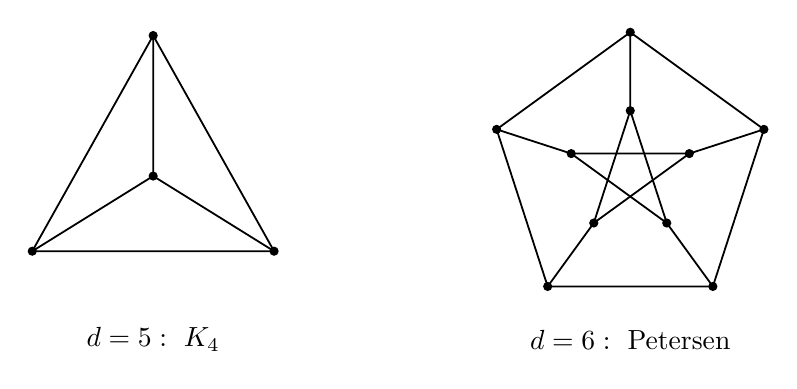
\begin{tikzpicture}[scale=0.83,line width=0.65pt]
\begin{scope}[xshift=-4cm]
\coordinate (a) at (0,2.1);\coordinate (b) at (-1.85,-1.2);
\coordinate (c) at (1.85,-1.2);\coordinate (d) at (0,-0.05);
\draw (a)--(b)--(c)--cycle;
\draw (d)--(a) (d)--(b) (d)--(c);
\foreach \x in {a,b,c,d}{\fill (\x) circle(2pt);}
\node at (0,-2.55) {$d=5:\ K_4$};
\end{scope}
\begin{scope}[xshift=3.3cm]
\foreach \i in {0,...,4}{
\coordinate (A\i) at ({90+72*\i}:2.15);
\coordinate (B\i) at ({90+72*\i}:0.95);}
\foreach \i in {0,...,4}{
\pgfmathtruncatemacro{\j}{mod(\i+1,5)}
\pgfmathtruncatemacro{\k}{mod(\i+2,5)}
\draw (A\i)--(A\j) (A\i)--(B\i) (B\i)--(B\k);
\fill (A\i) circle(2pt);\fill (B\i) circle(2pt);}
\node at (0,-2.55) {$d=6:\ \text{Petersen}$};
\end{scope}
\end{tikzpicture}
\caption{core頂点のlink。右は同時Petersen化した選択の一つ。右図の線分の内部交差はグラフの頂点を表さない。}
\label{fig:links}
\end{figure}

\subsection{通常の閉じたaffine surfaceとの区別}
\begin{corollary}\label{inv:no-almost-toric}
$d\ge5$の$X_d$は、境界のない通常の曲面を基底とし、focus--focus特異点だけを許すclosed almost toric fibrationを持たない。
\end{corollary}
\begin{proof}
Leung--Symingtonの分類\cite[Theorem 2.1, Table 1]{LeungSymington}では、この場合の全空間はK3、Enriques、または対応するtorus bundlesである。
そのEuler数はそれぞれ24、12、0である。
式\eqref{inv:euler}の値は$d\ge5$で55以上なので、いずれとも一致しない。
\end{proof}

定理\ref{main:global}が許すbranchとcoreは、この制約と両立している。
一方、coreの型を次数によらず有限個に制限できるか、分岐を含む底空間にどのtropical構造を与えられるかは、この構成の次に残る問題である。

\begin{thebibliography}{99}

\bibitem{AAK}
M. Abouzaid, D. Auroux and L. Katzarkov,
\emph{Lagrangian fibrations on blowups of toric varieties and mirror symmetry for hypersurfaces},
Publications Mathématiques de l'IHÉS \textbf{123} (2016), 199--282.
\url{https://doi.org/10.1007/s10240-016-0081-9}.

\bibitem{BSV}
M. S. Borman, N. Sheridan and U. Varolgunes,
\emph{Quantum cohomology as a deformation of symplectic cohomology},
Journal of Fixed Point Theory and Applications \textbf{24} (2022), article 48.
Proposition~2.10 (commuting Hamiltonians and adapted primitive).
\url{https://doi.org/10.1007/s11784-022-00965-6};
\url{https://arxiv.org/abs/2108.08391v2}.

\bibitem{CGblowup}
P. Chakravarthy and Y. Groman,
\emph{Almost toric fibrations on symplectic blow ups},
arXiv:2510.00994v1 (2025).
Theorem~1.1, Definition~2.2, Lemma~3.7.
\url{https://arxiv.org/abs/2510.00994v1}.

\bibitem{CGK3}
P. Chakravarthy and Y. Groman,
\emph{Almost toric fibrations on K3 surfaces via degenerations},
Advances in Mathematics \textbf{502} (2026), Part~B, 111138.
Definition~1.2, Theorems~1.6, 1.8, Corollary~1.9;
Lemma~2.13 is cited in the revised arXiv version of 28 May 2026.
\url{https://doi.org/10.1016/j.aim.2026.111138};
\url{https://arxiv.org/abs/2502.04304v3}.

\bibitem{DMT}
J.-P. Dufour, P. Molino and A. Toulet,
\emph{Classification des systèmes intégrables en dimension 2 et invariants des modèles de Fomenko},
Comptes Rendus de l'Académie des Sciences, Paris, Série~I, Mathématique
\textbf{318} (1994), no.~10, 949--952.
An English translation is available at
\url{https://webpages.csus.edu/mjv/DufourMolinoToulet.pdf}.

\bibitem{DHJH}
S. Dwivedi, J. Herman, L. C. Jeffrey and T. van den Hurk,
\emph{Hamiltonian Group Actions and Equivariant Cohomology},
SpringerBriefs in Mathematics, Springer, Cham, 2019.
Theorem~3.2 and Corollary~3.4, pp.~17--20 (symplectic neighborhood);
Chapter~10 (Duistermaat--Heckman).
\url{https://doi.org/10.1007/978-3-030-27227-2}.

\bibitem{Evans}
J. Evans,
\emph{Lectures on Lagrangian Torus Fibrations},
Cambridge University Press, Cambridge, 2023.
\url{https://arxiv.org/abs/2110.08643v4}.

\bibitem{EvansNotes}
J. Evans,
\emph{Lagrangian torus fibrations (notes in progress)},
8 February 2019.
Lemmas~6.1.5, 6.2.1 and \S6.3.
The numbering here refers to this preliminary set of notes, not to \cite{Evans}.
\url{https://jde27.uk/misc/ltf.pdf}.

\bibitem{EM}
J. D. Evans and M. Mauri,
\emph{Constructing local models for Lagrangian torus fibrations},
Annales Henri Lebesgue \textbf{4} (2021), 537--570.
Lemmas~2.16, 2.22, 3.1; Remarks~2.7, 2.19, 2.23; \S3.1;
Assumption~6.6, Proposition~6.13 and Theorem~6.15.
\url{https://doi.org/10.5802/ahl.80};
\url{https://arxiv.org/abs/1905.09229v3}.

\bibitem{EvansUrzua}
J. D. Evans and G. Urz\'ua,
\emph{Antiflips, mutations, and unbounded symplectic embeddings of rational homology balls},
Ann. Inst. Fourier \textbf{71} (2021), no.~5, 1807--1843.
\url{https://doi.org/10.5802/aif.3429}.

\bibitem{BHS}
J. Brendel, J. Hauber and J. Schmitz,
\emph{Semi-Local Exotic Lagrangian Tori in Dimension Four},
Ann. Inst. Fourier, online first (2026), 48 pp.
\url{https://doi.org/10.5802/aif.3789};
\url{https://arxiv.org/abs/2403.00408}.

\bibitem{FBP}
J. Fernández de Bobadilla and T. Pełka,
\emph{Fibrations by Lagrangian tori for maximal Calabi--Yau degenerations and beyond},
Communications on Pure and Applied Mathematics (2026), e70060,
published online 8 July 2026,
\url{https://doi.org/10.1002/cpa.70060}.
Theorem~6.14, Proposition~5.6, Example~5.8 and Remark~5.9 are cited from the final preprint,
arXiv:2312.13248v4, 9 July 2026.
\url{https://arxiv.org/abs/2312.13248v4}.

\bibitem{Fleming}
A. Fleming,
\emph{Kähler packings of projective complex manifolds},
European Journal of Mathematics \textbf{7} (2021), 1382--1400.
Proposition~4.6 and Construction~4.7.
\url{https://doi.org/10.1007/s40879-021-00491-8};
\url{https://arxiv.org/abs/1905.03140}.

\bibitem{Forstneric}
F. Forstnerič,
\emph{Euclidean domains in complex manifolds},
Journal of Mathematical Analysis and Applications \textbf{506} (2022), no.~1, 125660.
The Introduction recalls the holomorphic tubular-neighborhood theorem of Docquier--Grauert.
\url{https://doi.org/10.1016/j.jmaa.2021.125660};
\url{https://arxiv.org/abs/2104.03051v3}.

\bibitem{GollaMartelli}
M. Golla and B. Martelli,
\emph{Pair of pants decomposition of 4-manifolds},
Algebraic \& Geometric Topology \textbf{17} (2017), no.~3, 1407--1444.
\url{https://doi.org/10.2140/agt.2017.17.1407};
\url{https://arxiv.org/abs/1503.05839}.

\bibitem{GV}
Y. Groman and U. Varolgunes,
\emph{Locality of relative symplectic cohomology for complete embeddings},
Compositio Mathematica \textbf{159} (2023), no.~12, 2551--2637.
\S7.3, Lemma~7.19 and Proposition~7.21.
\url{https://doi.org/10.1112/S0010437X23007492};
\url{https://arxiv.org/abs/2110.08891v4}.

\bibitem{GrossSiebert}
M. Gross and B. Siebert,
\emph{From real affine geometry to complex geometry},
Annals of Mathematics (2) \textbf{174} (2011), no.~3, 1301--1428.
\url{https://doi.org/10.4007/annals.2011.174.3.1}.

\bibitem{Hatcher}
A. Hatcher,
\emph{Algebraic Topology},
Cambridge University Press, Cambridge, 2002.
\S\S0.2, 2.2 and 4.2 (CW complexes, cellular homology and homotopy equivalences).
\url{https://pi.math.cornell.edu/~hatcher/AT/ATpage.html}.

\bibitem{Hartshorne}
R. Hartshorne,
\emph{Algebraic Geometry},
Graduate Texts in Mathematics \textbf{52}, Springer, New York, 1977.
Chapter~V, Theorem~1.10 (the Nakai--Moishezon criterion for surfaces).
\url{https://doi.org/10.1007/978-1-4757-3849-0}.

\bibitem{Hattori}
A. Hattori,
\emph{Topology of $\mathbb C^n$ minus a finite number of affine hyperplanes in general position},
Journal of the Faculty of Science, University of Tokyo, Section~IA, Mathematics
\textbf{22} (1975), no.~2, 205--219.
\url{https://repository.dl.itc.u-tokyo.ac.jp/records/39761}.

\bibitem{IKM}
A. Izosimov, B. Khesin and M. Mousavi,
\emph{Coadjoint orbits of symplectic diffeomorphisms of surfaces and ideal hydrodynamics},
Annales de l'Institut Fourier \textbf{66} (2016), no.~6, 2385--2433.
Theorems~3.11 and 3.17 (measured Reeb graphs and weighted Reeb graphs).
\url{https://doi.org/10.5802/aif.3066};
\url{https://arxiv.org/abs/1504.05629}.

\bibitem{LeungSymington}
N. C. Leung and M. Symington,
\emph{Almost toric symplectic four-manifolds},
Journal of Symplectic Geometry \textbf{8} (2010), no.~2, 143--187.
Theorem~2.6 and Table~1.
\url{https://doi.org/10.4310/JSG.2010.v8.n2.a2};
\url{https://arxiv.org/abs/math/0312165}.

\bibitem{LeungWan}
N. C. Leung and T. Y. H. Wan,
\emph{Calabi--Yau components in general type hypersurfaces},
Journal of Differential Geometry \textbf{83} (2009), no.~1, 43--74.
\S\S1 and 3.1.
\url{https://doi.org/10.4310/jdg/1253804351};
\url{https://arxiv.org/abs/0807.1784}.

\bibitem{Maksymenko}
S. Maksymenko,
\emph{Path-components of Morse mappings spaces of surfaces},
Commentarii Mathematici Helvetici \textbf{80} (2005), no.~3, 655--690.
Main Theorem, Lemma~4.1 and \S6.3.
\url{https://doi.org/10.4171/CMH/30};
\url{https://arxiv.org/abs/math/9910085}.

\bibitem{MatessiPants}
D. Matessi,
\emph{Lagrangian pairs of pants},
International Mathematics Research Notices \textbf{2021} (2021), no.~15, 11306--11356.
\url{https://doi.org/10.1093/imrn/rnz126};
\url{https://arxiv.org/abs/1802.02993}.

\bibitem{Matessi}
D. Matessi,
\emph{Lagrangian submanifolds from tropical hypersurfaces},
International Journal of Mathematics \textbf{32} (2021), no.~7, 2150046, 63~pp.
\url{https://arxiv.org/abs/1804.01469}.

\bibitem{IvanSmithTorus}
I. Smith,
\emph{Torus fibrations on symplectic four-manifolds},
Turkish Journal of Mathematics \textbf{25} (2001), no.~1, 69--96.
\url{https://journals.tubitak.gov.tr/math/vol25/iss1/4/}.
分類の仮定は connected homologically essential Lagrangian tori と
tame singularities である（原論文のabstractと定理の射程を区別する）．

\bibitem{Mikhalkin}
G. Mikhalkin,
\emph{Decomposition into pairs-of-pants for complex algebraic hypersurfaces},
Topology \textbf{43} (2004), no.~5, 1035--1065.
Theorems~1 and~1$'$; \S4.2.
\url{https://doi.org/10.1016/j.top.2003.11.006};
\url{https://arxiv.org/abs/math/0205011v3}.

\bibitem{PapadimaSuciu}
S. Papadima and A. I. Suciu,
\emph{Higher homotopy groups of complements of complex hyperplane arrangements},
Advances in Mathematics \textbf{165} (2002), 71--100.
\S1.1 (Hattori's theorem for generic arrangements).
\url{https://arxiv.org/abs/math/0002251}.

\bibitem{Pascaleff}
J. Pascaleff,
\emph{On the symplectic cohomology of log Calabi--Yau surfaces},
Geometry \& Topology \textbf{23} (2019), no.~6, 2701--2792.
\S4.2.
\url{https://doi.org/10.2140/gt.2019.23.2701};
\url{https://arxiv.org/abs/1304.5298v3}.

\bibitem{Ruan}
W.-D. Ruan,
\emph{Lagrangian torus fibration of quintic hypersurfaces. I. Fermat quintic case},
in \emph{Winter School on Mirror Symmetry, Vector Bundles and Lagrangian Submanifolds}
(Cambridge, MA, 1999), AMS/IP Studies in Advanced Mathematics \textbf{23},
American Mathematical Society, Providence, RI, 2001, 297--332.
\url{https://arxiv.org/abs/math/9904012}.

\bibitem{RSTZ}
H. Ruddat, N. Sibilla, D. Treumann and E. Zaslow,
\emph{Skeleta of affine hypersurfaces},
Geometry \& Topology \textbf{18} (2014), no.~3, 1343--1395.
\url{https://doi.org/10.2140/gt.2014.18.1343};
\url{https://arxiv.org/abs/1211.5263}.

\bibitem{StacksAmpleness}
The Stacks Project Authors,
\emph{The Stacks Project}, 2026.
Lemma~30.17.2, Tag~0B5V (ampleness under finite surjective pullback);
Lemma~37.50.3, Tag~0D2S (relative ampleness near an ample fiber);
Lemma~71.15.3, Tag~0D3A (the algebraic-space version).
\url{https://stacks.math.columbia.edu/tag/0B5V};
\url{https://stacks.math.columbia.edu/tag/0D2S};
\url{https://stacks.math.columbia.edu/tag/0D3A}.

\bibitem{VuNgoc}
S. Vũ Ngọc,
\emph{On semi-global invariants for focus--focus singularities},
Topology \textbf{42} (2003), no.~2, 365--380.
Theorem~2.1 and \S3.
\url{https://doi.org/10.1016/S0040-9383(01)00026-X};
\url{https://arxiv.org/abs/math/0208245}.

\bibitem{Zhang}
Y. Zhang,
\emph{Pair-of-Pants Decompositions of 4-Manifolds Diffeomorphic to General Type Hypersurfaces},
Journal of Mathematical Study \textbf{58} (2025), no.~2, 211--252.
Theorem~1.1; the quintic example in \S1.
\url{https://doi.org/10.4208/jms.v58n2.25.06};
\url{https://arxiv.org/abs/2102.10037}.

\bibitem{Zhou}
P. Zhou,
\emph{Lagrangian skeleta of hypersurfaces in $(\mathbb C^*)^n$},
Selecta Mathematica (N.S.) \textbf{26} (2020), no.~2, article~26, 33~pp.
\url{https://arxiv.org/abs/1803.00320}.

% Bibliography for the SNC theorem and subsequent applications.

\bibitem{DGMS}
P. Deligne, P. Griffiths, J. Morgan and D. Sullivan,
\emph{Real homotopy theory of K\"ahler manifolds},
Inventiones Mathematicae \textbf{29} (1975), no.~3, 245--274.
Lemma~(5.11), pp.~266--267, and Remark~(5.14).
\url{https://doi.org/10.1007/BF01389853};
\url{https://www.math.stonybrook.edu/~dennis/publications/PDF/DS-pub-0024.pdf}.

\bibitem{TMZ}
M. Farajzadeh Tehrani, M. McLean and A. Zinger,
\emph{Normal crossings singularities for symplectic topology},
Advances in Mathematics \textbf{339} (2018), 672--748.
Definitions~2.8, 2.9, 2.11, 2.12 and Theorem~2.13.
\url{https://doi.org/10.1016/j.aim.2018.09.035};
\url{https://arxiv.org/abs/1410.0609v3}.

\bibitem{FeichtnerSturmfels}
Eva Maria Feichtner and Bernd Sturmfels,
\emph{Matroid polytopes, nested sets and Bergman fans},
Portugaliae Mathematica (N.S.) \textbf{62} (2005), no.~4, 437--468.
\href{https://arxiv.org/abs/math/0411260}{arXiv:math/0411260}.

\bibitem{ArdilaKlivans}
Federico Ardila and Caroline J. Klivans,
\emph{The Bergman complex of a matroid and phylogenetic trees},
Journal of Combinatorial Theory, Series B \textbf{96} (2006), no.~1, 38--49.
\href{https://doi.org/10.1016/j.jctb.2005.06.004}{doi:10.1016/j.jctb.2005.06.004}.
\href{https://arxiv.org/abs/math/0311370}{arXiv:math/0311370}.

\bibitem{Shaw}
Kristin M. Shaw,
\emph{A tropical intersection product in matroidal fans},
SIAM Journal on Discrete Mathematics \textbf{27} (2013), no.~1, 459--491.
\href{https://doi.org/10.1137/110850141}{doi:10.1137/110850141}.
\href{https://arxiv.org/abs/1010.3967v2}{arXiv:1010.3967v2}.

\bibitem{KapranovChow}
Mikhail M. Kapranov,
\emph{Chow quotients of Grassmannians. I},
in \emph{I.~M.~Gelfand Seminar},
Advances in Soviet Mathematics, vol.~16, part~2,
American Mathematical Society, Providence, RI, 1993, pp.~29--110.
\href{https://arxiv.org/abs/alg-geom/9210002}{arXiv:alg-geom/9210002}.

\bibitem{Aksnes}
E. Aksnes,
\emph{Tropicalization of curve arrangement complements and arroids},
Mathematica Scandinavica \textbf{131} (2025), no.~2.
\url{https://doi.org/10.7146/math.scand.a-156674};
\url{https://arxiv.org/abs/2404.14380v3}.

\bibitem{GKM}
A. Gathmann, M. Kerber and H. Markwig,
\emph{Tropical fans and the moduli spaces of tropical curves},
Compositio Mathematica \textbf{145} (2009), no.~1, 173--195.
\url{https://doi.org/10.1112/S0010437X08003837};
\url{https://arxiv.org/abs/0708.2268v2}.

\bibitem{MichalakReeb}
\L{}. P. Michalak,
\emph{Realization of a graph as the Reeb graph of a Morse function on a manifold},
Topological Methods in Nonlinear Analysis \textbf{52} (2018), no.~2, 749--762.
Definition~2.2 and Theorem~5.6.
\url{https://doi.org/10.12775/TMNA.2018.029};
\url{https://arxiv.org/abs/1805.06727v2}.

% Add this entry inside the main thebibliography environment.

\bibitem{ShawSurfaces}
Kristin Shaw,
\emph{Tropical surfaces},
arXiv:1506.07407v1 (2015), 43 pp.
Definition~3.1, pp.~15--16 (ambient integer affine transitions);
\S3.2 (boundary), \S4.2 (tropical summation).
\url{https://arxiv.org/abs/1506.07407v1};
\url{https://arxiv.org/pdf/1506.07407}.

\bibitem{JellRauShaw}
Philipp Jell, Johannes Rau, and Kristin Shaw,
\emph{Lefschetz $(1,1)$-theorem in tropical geometry},
\'Epijournal de G\'eom\'etrie Alg\'ebrique \textbf{2} (2018), Article~11, 27 pp.
Definitions~2.1, 3.1 and 5.1 (rational polyhedral spaces, the affine sheaf, and matroidal charts).
\url{https://doi.org/10.46298/epiga.2018.volume2.4126};
\url{https://epiga.episciences.org/4981/pdf};
\url{https://arxiv.org/abs/1711.07900}.

\bibitem{LRSChern}
Luc\'ia L\'opez de Medrano, Felipe Rinc\'on, and Kris Shaw,
\emph{Chern Classes of Tropical Manifolds},
arXiv:2309.00229v2 (2023), 30 pp.
Definitions~2.2--2.4, pp.~4--5 (extended integer affine maps, tropical manifold atlas, and boundary).
\url{https://arxiv.org/abs/2309.00229v2};
\url{https://arxiv.org/pdf/2309.00229}.

\bibitem{CartwrightComplexes}
Dustin Cartwright,
\emph{Tropical complexes},
Manuscripta Mathematica \textbf{163} (2020), 227--261.
Proposition~2.1; Lemma~2.2; Definitions~2.5, 2.8;
Proposition~2.10; Construction~3.2 and Remark~3.4.
The linked arXiv version is v4 (2019).
\url{https://doi.org/10.1007/s00229-019-01148-3};
\url{https://arxiv.org/abs/1308.3813v4};
\url{https://arxiv.org/pdf/1308.3813}.

% Existing EM entry can additionally mention Assumption 6.6,
% Proposition 6.13 and Theorem 6.15.  Their log Calabi--Yau hypotheses
% must remain explicit; they do not prove the present branched atlas.
% Existing VuNgoc entry can additionally mention Remark 3.1,
% which displays the focus--focus monodromy matrix.

\bibitem{ShawWerner}
K. Shaw and A. Werner,
\emph{On the birational geometry of matroids},
Combinatorial Theory \textbf{3} (2023), no.~2, Paper No.~17.
Theorem~7.2 (parallel connections and product Bergman fans).
\url{https://doi.org/10.5070/C63261996};
\url{https://arxiv.org/abs/2207.13639v1}.

\bibitem{AllermannRau}
L. Allermann and J. Rau,
\emph{First steps in tropical intersection theory},
Mathematische Zeitschrift \textbf{264} (2010), no.~3, 633--670.
Definition~3.4, Remark~3.5, Proposition~3.7;
Definition~6.1 and Construction~6.4.
\url{https://doi.org/10.1007/s00209-009-0483-1};
\url{https://arxiv.org/abs/0709.3705v3}.

\bibitem{SymingtonFour}
M. Symington,
\emph{Four dimensions from two in symplectic topology},
arXiv:math/0210033v1 (2002).
Proposition~2.15, \S4.3, equation~(4.10), and Proposition~4.14.
\url{https://arxiv.org/abs/math/0210033v1}.

\bibitem{QuinticArithmetic}
\emph{五次曲面の整数アフィン接着と高分母支持グラフ}，
未発表草稿，第25稿，2026年10月28日．
本稿の companion 論文．


\bibitem{RuddatAnnouncement2026}
H. Ruddat,
\emph{Lagrangian torus fibrations of Calabi--Yau hypersurfaces},
Institut Mittag--Leffler, seminar abstract, 30 June 2026.
Joint work with C. Y. Mak, D. Matessi and I. Zharkov, as stated in the abstract.
Announcement; accessed 28 October 2026.
\url{https://www.mittag-leffler.se/seminar/helge-ruddat-tba/}.

\bibitem{ZharkovSoftCells2026}
I. Zharkov,
\emph{Phase Tropical hypersurfaces and their cousins},
ICMS--Sofia Geometry Seminar, 15 April 2026; announcement posted 8 April 2026.
Seminar abstract; accessed 28 October 2026.
\href{https://icms.bg/phase-tropical-hypersurfaces-and-their-cousins-geometry-seminar-talk-by-ilia-zharkov/}{ICMS--Sofia: seminar announcement}.


\bibitem{VenugopalanWoodward2026}
S. Venugopalan and C. T. Woodward,
\emph{Tropical disk potential for almost toric manifolds},
arXiv:2604.03161v1, 3 April 2026.
Definitions~1.1--1.2, Theorem~1.3, and the discussion of the nonmonotone potential in \S1.
\url{https://arxiv.org/abs/2604.03161v1}.

\bibitem{ZhangNegativeKE}
Y. Zhang,
\emph{Collapsing of negative Kähler--Einstein metrics},
Mathematical Research Letters \textbf{22} (2015), no.~6, 1843--1869.
\url{https://doi.org/10.4310/MRL.2015.v22.n6.a16}.
Theorems~1.1, 2.4, 2.6 in \url{https://arxiv.org/abs/1505.04728v2}.

\bibitem{SongNegativeKE}
J. Song,
\emph{Degeneration of Kähler--Einstein manifolds of negative scalar curvature},
arXiv:1706.01518v1 (2017), Theorem~1.2.
\url{https://arxiv.org/abs/1706.01518}.

\bibitem{MandelNegativeKE}
H. Mandel,
\emph{Degenerations of negative Kähler--Einstein surfaces},
Journal of the London Mathematical Society \textbf{109} (2024), no.~1, e12818.
\url{https://doi.org/10.1112/jlms.12818}.

\bibitem{KECubicalCurrent}
K. Ueda,
\emph{多重スケール Kähler--Einstein 幾何 V：超平面和への退化，立方体極限，および直径},
現行未公表原稿．定理 \texttt{thm:degree-d-limit}，
仮定 \texttt{hyp:CPd}, \texttt{hyp:PBEd}．
\url{https://github.com/uedakazushi/kaehler-einstein-degeneration/blob/main/papers/cubical-gh-limit.tex}.

\bibitem{RuanHMinimal}
W.-D. Ruan,
\emph{H-minimal Lagrangian fibrations in Kähler manifolds and minimal
Lagrangian vanishing tori in Kähler--Einstein manifolds},
arXiv:math/0309177v2 (2003).
Proposition~3.1, Lemma~3.3, and Theorems~3.1, 4.2.
\url{https://arxiv.org/abs/math/0309177v2}.

\bibitem{KELocalCurrent}
K. Ueda,
\emph{多重スケール Kähler--Einstein 幾何 IV：超平面和への退化と局所模型},
現行未公表原稿．
\texttt{coarse:hyp:TC5}，
\texttt{coarse:prop:density-counterexample}，
\texttt{coarse:lem:actual-buffer-comparison}．
\url{https://github.com/uedakazushi/kaehler-einstein-degeneration/blob/main/papers/kaehler-einstein-degeneration.tex}.

\end{thebibliography}

\end{document}
